\documentclass[12pt,a4paper,english,twoside]{book}
\usepackage[german,english]{babel}
\usepackage[T1]{fontenc} 
\usepackage[utf8]{inputenc}
\usepackage{amsfonts}
\usepackage{amsmath}
\usepackage{latexsym}
\usepackage{amssymb}
\usepackage{epsfig}
\usepackage{moreverb}
\usepackage{rotating}
\usepackage{enumerate}
\usepackage{graphics, graphicx,wrapfig}
\usepackage{subcaption}
\usepackage{fancybox}
\usepackage{picinpar,varioref,floatflt}
\usepackage{ae}
\usepackage{longtable}
\usepackage{booktabs}
\usepackage{textcomp}
\usepackage{float}
\usepackage{url}
\usepackage{unizhdt}
\usepackage{csvsimple}
% newly added
\usepackage{listings}
\usepackage{hyperref}
%\usepackage{parskip} 

\renewcommand{\labelitemi}{\labelitemfont$\bullet$}
\newcommand{\degree}{$^\circ$}
\newcommand{\degreem}{^\circ}

%table sachen
\usepackage{multirow} % For multirows
\usepackage{amssymb} % For the checkmark
\usepackage{graphicx} % For the rotation
\usepackage{array} % To enlarge the vertical space of the table's contents
\usepackage{tabularx}
\usepackage{caption,tabularx,booktabs}


\makeatletter
\newenvironment{CenteredBox}{% 
\begin{Sbox}}{% Save the content in a box
\end{Sbox}\centerline{\parbox{\wd\@Sbox}{\TheSbox}}}% And output it centered
\makeatother

\usepackage{color}
\usepackage[table,xcdraw]{xcolor}
\definecolor{lightgray}{rgb}{.9,.9,.9}
\definecolor{darkgray}{rgb}{.4,.4,.4}
\definecolor{purple}{rgb}{0.65, 0.12, 0.82}
\definecolor{darkgreen}{RGB}{30, 142, 20}

\lstdefinelanguage{JavaScript}{
	keywords={typeof, new, true, false, catch, function, return, null, catch, switch, let, var, if, in, while, do, else, case, break, async, await, const},
	keywordstyle=\color{purple}\bfseries,
	ndkeywords={class, export, boolean, throw, implements, import, this},
	ndkeywordstyle=\color{darkgray}\bfseries,
	identifierstyle=\color{black},
	sensitive=false,
	comment=[l]{//},
	morecomment=[s]{/*}{*/},
	commentstyle=\color{darkgreen}\ttfamily,
	stringstyle=\color{darkgreen}\ttfamily,
	morestring=[b]',
	morestring=[b]"
}

\lstset{
	language=JavaScript,
	extendedchars=true,
	basicstyle=\footnotesize\ttfamily,
	showstringspaces=false,
	showspaces=false,
	numbers=left,
	numberstyle=\footnotesize,
	numbersep=9pt,
	tabsize=2,
	breaklines=true,
	showtabs=false,
	captionpos=b
}

%%%%%%%%%%%%%%%%%%%%%%%%%%%%%%%%%%%%%%%%%%%%%%%%%%

% Define the language of the diploma thesis
\selectlanguage{english}
%\selectlanguage{german}

\pagestyle{headings}

\begin{document}

%%%%%%%%%%%%%%%%%%%%%%%%%%%%%%%%%%%%%%%%%%%%%%%%%%

% Define the author printed on the cover page
\author{Name Lastname}
% Define the city and country of the author
\authorcity{Zurich, Switzerland}
% Define the student ID (Matrikelnummer)
\studentid{TBD}
% Define the title with optional subtitle
\title{MTT: My Thesis Title}
% Define the supervisors
\supervisors{Name Lastname, Name Lastname, Prof. Dr. Burkhard Stiller}
% Define the submission date
\submissiondate{Month DD, YYYY}

%%%%%%%%%%%%%%%%%%%%%%%%%%%%%%%%%%%%%%%%%%%%%%%%%%

% Make the title page
\maketitle

% Make the imprint on the back of the cover page
\makeimprint

\pagenumbering{roman}

% Include the files of the diploma thesis
%\cleardoublepage
\chapter*{Declaration of Independence}
\addcontentsline{toc}{chapter}{Declaration of Independence}
I hereby declare that I have composed this work independently and without the use of any aids other than those declared (including generative AI such as ChatGPT). I am aware that I take full responsibility for the scientific character of the submitted text myself, even if AI aids were used and declared (after written confirmation by the supervising professor). All passages taken verbatim or in sense from published or unpublished writings are identified as such. The work has not yet been submitted in the same or similar form or in excerpts as part of another examination.

\vspace{2cm}

Z{\"u}rich, \hspace{5cm} \hrulefill \\
\hspace*{6.4cm} Signature of student
\chapter*{Abstract}
\addcontentsline{toc}{chapter}{Abstract}


%===============================================================================
%%%%%%%%%%%%%%%%%%%%%%%%%%%%%%%%
% Recipe to do an abstract:
%%%%%%%%%%%%%%%%%%%%%%%%%%%%%%%%
%(1) Context
%(2) Research Gap
%(3) Goals, Objectives
%(4) Methodology, how
%(5) Results

% Example:
%Abstract
%(1) In the context of energy efficiency in computer networks, a significant number of solutions ranging from protocols and functionalities to energy efficiency-oriented management applications have been proposed. 
%(2) However, the characteristics of environments to develop and validate such solutions are not as discussed as the solutions themselves. 
%(3) Considering this, this work proposes an emulation environment to develop and validate energy efficiency-oriented solutions, as well as discuss their specific characteristics. 
%(4) Thus, three functionalities of different network scopes are implemented, Adaptive Link Rate (interface level), Syncronized Coalescing (device level) and SustNMS (network level) in the Mininet emulation environment using the implemented software-defined networks paradigm on the POX controller. 
%(5) The environment is validated by comparing the energy savings achieved by these features in a topology inspired by the National Research Network (RNP).

\selectlanguage{german}

%
% Blablabla
%

\newpage
\selectlanguage{english}

%
% Blablabla
%








%\cleardoublepage
\chapter*{Acknowledgments}
\addcontentsline{toc}{chapter}{Acknowledgments}


\tableofcontents
\cleardoublepage
\pagenumbering{arabic}
% --------------
% Body
% --------------
\chapter{Introduction}
\label{introduction}


Artworks are sensitive to many externalfactors, such as humidity, temperature and vibrations.
While these factors are generally well controlled for in museums and storage, artpieces need also be moved between these buildings.
Artworks include a variety of objects, ranging from photographs and paintings the variety of pieces needed for modern installations.
The transportation therefore needs to be secure and flexible.
Sensors play a critical role in the safe transportation of these objects.


\section{Motivation}

Certify is an international cooperative project between twelve partners situated in Switzerland and the EU %\citep{Brüschre von certify}.
One of those partners is the university of zurich.
Its focus is on the development of Internet of Things (IoT) systems for security, monitoring and detection %\citep{Brüschüre von certify}.
Next to certifications and the development of frameworks, Certify also consirnes itself with the integration of IoT devices.


One of multiple currently running pilots of Certify is the "Tracking and monitoring of artworks" %\citep{https://certify-project.eu/pilots/}.
The goal of this pilot is to enable the constant tracking and monitoring of artworks by attaching a device to it.
This device allows for unique identification, by using cryptographic methods.
It is also intended to act as a cluster of sensors that collect information about the surounding of the artwork that are relevant to the wellbeeing of the artwork.
The goal is to have constant data on the artwork throughout its lifecycle.
This is intended to help with securing the artwork and helping with chain of custody monitoring.



\section{Thesis Goals}

The goal of this project is to develop a system that implements a localized version of the artwork tracking envisioned by the Certify project, ment for transportation in a truck.
Additionally the system will extend the Certify Projects goal by adding new detection methods and also informs the driver of the truck about potential problems.

The goal is to develop a system that tracks the state of artwork in a truck using different detection methods.
The devices attached to the artworks, called tags, build a local decentralized network.
The phone of the driver can query the network and displayed the collected metrics to them.
If a metric is outside of the accepted norm, the system should allert the driver.

This thesis presents a proof of concept implementation.
The used metrics are not intended to be a full representation of needed sensors to securley Transport art.
Rather they are intended to show different types of sensors that can be used.
This thesis assumes that the data transfer to a server using 4G, as planned by the Certify project, will work and will not implement it in this thesis.



\section{Methodology}

This Thesis was made in four stages:

\subsubsection{Reserach}
In a first step, the basis of the thesis had to be researched.
This involved familiarizing with existing research on the toping of artwork tracking, local IoT networks and commonly used communication protocols.
Existing artwork tracking methods need to be analyzed and evaluated, considering their strength and shortcommings during the transportation in a truck.
The types of sensors that could be relevant need to be chosen, based on existing research, cost and avaliablity.
Options for the network-architecture inside the truck needed to be researched and compared, based on performance, stability and security.
A communication protocol needed to be chosen, based on the same criterias.

\subsubsection{Design}
Once the fundamental knowledge for the project had been aquired, the system had to be designed.
The design was chosen based on feasability, security and stability.

\subsubsection{Implementation}
The desig then was implemented in a simplified manner based on the material that was avaliable.
For this four tags were build, equiped with sensors, communication-capabilities and power suply.
Then the required software was written, using existing implementations when possible and writing new code when required.
A simple example app was also developed, based on an existing communications app published by Nordic Semiconductors and installed on a phone.

\subsubsection{Evaluation}
The developed system of tags and phone was tested in a series of five experiments.
The first four experiments were intended to caputre a specific part of the system, while the last was a general purpose test.
The tests were performed in a manner that insured minimal external influence.
The resulting data from the testswere analyzed using statistical methods.
The goal was to determin the reliability of the system, find limitations and look for emprovements.

\section{Thesis Outline}

This thesis is structured as follows:

Chapter two presents fundamental knowledge researched for this thesis. 
Additionaly chapter two also present previous research done, related to the tracking of artwork and sensor networks.
Chapter three presents the design of the system and its inner workings and capabilities.
Chapter four shows the implementation that was developed and used for this project.
Chapter five decsibes the experiments performed. It presents the results of the experiments and discusses them.
chapter six summarizes the finding of this thesis and discusses the most important aspects in a conclusion.


%\chapter{Introduction}
\label{introduction}


Artworks are sensitive to many externalfactors, such as humidity, temperature and vibrations.
While these factors are generally well controlled for in museums and storage, artpieces need also be moved between these buildings.
Artworks include a variety of objects, ranging from photographs and paintings the variety of pieces needed for modern installations.
The transportation therefore needs to be secure and flexible.
Sensors play a critical role in the safe transportation of these objects.


\section{Motivation}

Certify is an international cooperative project between twelve partners situated in Switzerland and the EU %\citep{Brüschre von certify}.
One of those partners is the university of zurich.
Its focus is on the development of Internet of Things (IoT) systems for security, monitoring and detection %\citep{Brüschüre von certify}.
Next to certifications and the development of frameworks, Certify also consirnes itself with the integration of IoT devices.


One of multiple currently running pilots of Certify is the "Tracking and monitoring of artworks" %\citep{https://certify-project.eu/pilots/}.
The goal of this pilot is to enable the constant tracking and monitoring of artworks by attaching a device to it.
This device allows for unique identification, by using cryptographic methods.
It is also intended to act as a cluster of sensors that collect information about the surounding of the artwork that are relevant to the wellbeeing of the artwork.
The goal is to have constant data on the artwork throughout its lifecycle.
This is intended to help with securing the artwork and helping with chain of custody monitoring.



\section{Thesis Goals}

The goal of this project is to develop a system that implements a localized version of the artwork tracking envisioned by the Certify project, ment for transportation in a truck.
Additionally the system will extend the Certify Projects goal by adding new detection methods and also informs the driver of the truck about potential problems.

The goal is to develop a system that tracks the state of artwork in a truck using different detection methods.
The devices attached to the artworks, called tags, build a local decentralized network.
The phone of the driver can query the network and displayed the collected metrics to them.
If a metric is outside of the accepted norm, the system should allert the driver.

This thesis presents a proof of concept implementation.
The used metrics are not intended to be a full representation of needed sensors to securley Transport art.
Rather they are intended to show different types of sensors that can be used.
This thesis assumes that the data transfer to a server using 4G, as planned by the Certify project, will work and will not implement it in this thesis.



\section{Methodology}

This Thesis was made in four stages:

\subsubsection{Reserach}
In a first step, the basis of the thesis had to be researched.
This involved familiarizing with existing research on the toping of artwork tracking, local IoT networks and commonly used communication protocols.
Existing artwork tracking methods need to be analyzed and evaluated, considering their strength and shortcommings during the transportation in a truck.
The types of sensors that could be relevant need to be chosen, based on existing research, cost and avaliablity.
Options for the network-architecture inside the truck needed to be researched and compared, based on performance, stability and security.
A communication protocol needed to be chosen, based on the same criterias.

\subsubsection{Design}
Once the fundamental knowledge for the project had been aquired, the system had to be designed.
The design was chosen based on feasability, security and stability.

\subsubsection{Implementation}
The desig then was implemented in a simplified manner based on the material that was avaliable.
For this four tags were build, equiped with sensors, communication-capabilities and power suply.
Then the required software was written, using existing implementations when possible and writing new code when required.
A simple example app was also developed, based on an existing communications app published by Nordic Semiconductors and installed on a phone.

\subsubsection{Evaluation}
The developed system of tags and phone was tested in a series of five experiments.
The first four experiments were intended to caputre a specific part of the system, while the last was a general purpose test.
The tests were performed in a manner that insured minimal external influence.
The resulting data from the testswere analyzed using statistical methods.
The goal was to determin the reliability of the system, find limitations and look for emprovements.

\section{Thesis Outline}

This thesis is structured as follows:

Chapter two presents fundamental knowledge researched for this thesis. 
Additionaly chapter two also present previous research done, related to the tracking of artwork and sensor networks.
Chapter three presents the design of the system and its inner workings and capabilities.
Chapter four shows the implementation that was developed and used for this project.
Chapter five decsibes the experiments performed. It presents the results of the experiments and discusses them.
chapter six summarizes the finding of this thesis and discusses the most important aspects in a conclusion.


%\chapter{Introduction}
\label{introduction}


Artworks are sensitive to many externalfactors, such as humidity, temperature and vibrations.
While these factors are generally well controlled for in museums and storage, artpieces need also be moved between these buildings.
Artworks include a variety of objects, ranging from photographs and paintings the variety of pieces needed for modern installations.
The transportation therefore needs to be secure and flexible.
Sensors play a critical role in the safe transportation of these objects.


\section{Motivation}

Certify is an international cooperative project between twelve partners situated in Switzerland and the EU %\citep{Brüschre von certify}.
One of those partners is the university of zurich.
Its focus is on the development of Internet of Things (IoT) systems for security, monitoring and detection %\citep{Brüschüre von certify}.
Next to certifications and the development of frameworks, Certify also consirnes itself with the integration of IoT devices.


One of multiple currently running pilots of Certify is the "Tracking and monitoring of artworks" %\citep{https://certify-project.eu/pilots/}.
The goal of this pilot is to enable the constant tracking and monitoring of artworks by attaching a device to it.
This device allows for unique identification, by using cryptographic methods.
It is also intended to act as a cluster of sensors that collect information about the surounding of the artwork that are relevant to the wellbeeing of the artwork.
The goal is to have constant data on the artwork throughout its lifecycle.
This is intended to help with securing the artwork and helping with chain of custody monitoring.



\section{Thesis Goals}

The goal of this project is to develop a system that implements a localized version of the artwork tracking envisioned by the Certify project, ment for transportation in a truck.
Additionally the system will extend the Certify Projects goal by adding new detection methods and also informs the driver of the truck about potential problems.

The goal is to develop a system that tracks the state of artwork in a truck using different detection methods.
The devices attached to the artworks, called tags, build a local decentralized network.
The phone of the driver can query the network and displayed the collected metrics to them.
If a metric is outside of the accepted norm, the system should allert the driver.

This thesis presents a proof of concept implementation.
The used metrics are not intended to be a full representation of needed sensors to securley Transport art.
Rather they are intended to show different types of sensors that can be used.
This thesis assumes that the data transfer to a server using 4G, as planned by the Certify project, will work and will not implement it in this thesis.



\section{Methodology}

This Thesis was made in four stages:

\subsubsection{Reserach}
In a first step, the basis of the thesis had to be researched.
This involved familiarizing with existing research on the toping of artwork tracking, local IoT networks and commonly used communication protocols.
Existing artwork tracking methods need to be analyzed and evaluated, considering their strength and shortcommings during the transportation in a truck.
The types of sensors that could be relevant need to be chosen, based on existing research, cost and avaliablity.
Options for the network-architecture inside the truck needed to be researched and compared, based on performance, stability and security.
A communication protocol needed to be chosen, based on the same criterias.

\subsubsection{Design}
Once the fundamental knowledge for the project had been aquired, the system had to be designed.
The design was chosen based on feasability, security and stability.

\subsubsection{Implementation}
The desig then was implemented in a simplified manner based on the material that was avaliable.
For this four tags were build, equiped with sensors, communication-capabilities and power suply.
Then the required software was written, using existing implementations when possible and writing new code when required.
A simple example app was also developed, based on an existing communications app published by Nordic Semiconductors and installed on a phone.

\subsubsection{Evaluation}
The developed system of tags and phone was tested in a series of five experiments.
The first four experiments were intended to caputre a specific part of the system, while the last was a general purpose test.
The tests were performed in a manner that insured minimal external influence.
The resulting data from the testswere analyzed using statistical methods.
The goal was to determin the reliability of the system, find limitations and look for emprovements.

\section{Thesis Outline}

This thesis is structured as follows:

Chapter two presents fundamental knowledge researched for this thesis. 
Additionaly chapter two also present previous research done, related to the tracking of artwork and sensor networks.
Chapter three presents the design of the system and its inner workings and capabilities.
Chapter four shows the implementation that was developed and used for this project.
Chapter five decsibes the experiments performed. It presents the results of the experiments and discusses them.
chapter six summarizes the finding of this thesis and discusses the most important aspects in a conclusion.


%\input{chapters/introduction}
%\input{chapters/fundamentals}
%\input{chapters/design}
%\input{chapters/implementation}
%\input{chapters/evaluation}
%\input{chapters/considerations}

%\chapter{Fundamentals}

\section{Background}


\subsection{Ultra Wideband}

\subsubsection{IEEE}

The Ultra Wideband (UWB) communication protocoll was introduced in 2003 by the Institute of Electrical and Electronics Engineers (IEEE) as part of the IEEE 802.15.4 standard.
In 2020 updates were made to the protocoll when the IEEE 802.15.4z-2020 standard made improvements to the PHY layers of UWB connections. %“IEEE standard for low-rate wireless networks–amendment 1: Enhanced ultra wideband (UWB) physical layers (PHYs) and associated ranging techniques,” IEEE, C/LM - LAN/MAN Standards Committee, 2020
It achieved this by introducing a more robust timestamping system on the PHY layer.
This is suplemented by changes to the MAC layer, that allow for the exchange of ranging information.
The result is short frames, that are transmitted fast, between devices, leading to short bursts of communications that are fast, secure and ideal for ranging.


UWB works by using short radio frequency pulses, resulting in a large bandwidth.
UWB is a lower power communication form.
This prevents it from interfering with other communication forms it is sharing its wavelength with, such as WLAN or Bluetooth. 
Since UWB uses very short, distinc pulses over a short range, it has found use in ranging systems. %E. Hsu, “An overview of the IEEE 802.15.4 HRP UWB standard.” https:// blogs.keysight.com/ blogs/ tech/ rfmw.entry.html/ 2021/ 07/ 28/ an overview of IEEE-J7ac.html , 2021. (Accessed: 2022-12-22).
UWB is split into high rate pulse (HRP) UWB and low rate pulse (LRP) UWB.
Since ranging is part of this work and LRP is generally not used for ranging, I will not discuss it further in this thesis. %E. Hsu, “An overview of the IEEE 802.15.4 HRP UWB standard.” https:// blogs.keysight.com/ blogs/ tech/ rfmw.entry.html/ 2021/ 07/ 28/ an overview of IEEE-J7ac.html , 2021. (Accessed: 2022-12-22).
Since UWB devices tend to be small and have a low energy consumption, in combination with the capability of ranging as well as data transfer, they have become popular as Internet of Things (IoT) devices. \\ 

The standard defines the PHY and MAC layer as well as frequency bands for communication.
The 4z expansion tries to integrate UWB into the the WPAN standard. In Section ... and ... I will discuss the PHY and MAC layer.\\

The sending devices emits pulses in a pre-set band of frequencies, using short bursts to transmit the bits.
The signal forms a concave curve in this band, where the two points that are 10 db below the maximum power spectral density are called the lower- and upper-frequency point, see Figure \ref{f:UWB_spectrum}.
These two points must at least 500 Hz apart.
The maximum power spectral density must be below the noise level.
This process prevents conflicts with other communications, that use a single frequency with a high power spectral density and modulate signal transmission, such as WI-FI or Bluetooth.
The UWB protocol has the added benefit of being useful for high accuracy localization.


\begin{figure}[ht!]
\centering
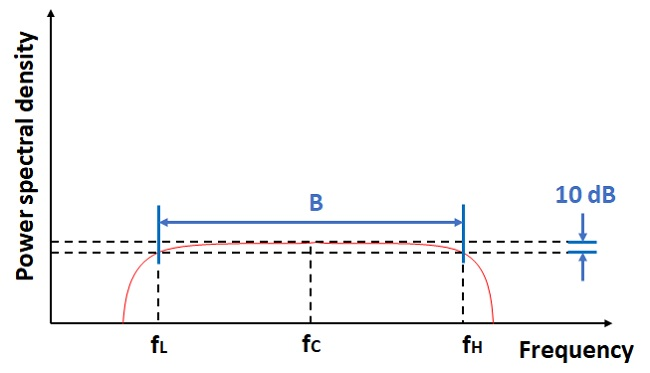
\includegraphics[width=\linewidth]{graphics/UWB_spectrum.jpg}
\caption{Power Spectral Density: Bandwidth B, lower-frequency f\textsubscript{L}, upper-frequency f\textsubscript{H}, \cite{hsu_2021}}
\label{f:UWB_spectrum}
\end{figure}


\subsubsection{UWB supported Nodes}

The IEEE 802.15.4 standard distinquishes between two types of devices.
Full-function device (FFD) are capable of connecting to multiple other devices, receive, transmit and coordinate. Reduced-function device (RFD) on the other hand can only connect to one other device and act as worker. 
In Topological terms RFDs can only operate as leaves, while FFDs can be any node in a network, including leaves.
RFDs therefore are strictly worse, but make up for it by requiering fewer resources, such as memory and power.
When FFDs work as PAN coordinators, they can use short adresses to address any node.
The PAN also has a PAN identifier, to help communication accross multiple networks, while still using the short address.
Each device also has a extended address, that is not assigned by any coordinator, that serves as a universal unique identifier (UUID).


\subsection{UWB MAC}
\label{sec:UWB MAC}

The Mac Layer is part of the Data link layer.
The Mac Frame is the payload of the PHY frame. It carries information about the type of frame, frame-format, security mechanism, adressing and frame validation.
The Mac Layer additionaly provides rules for beacon managment, chanel access.

\begin{figure}[ht!]
	\centering
	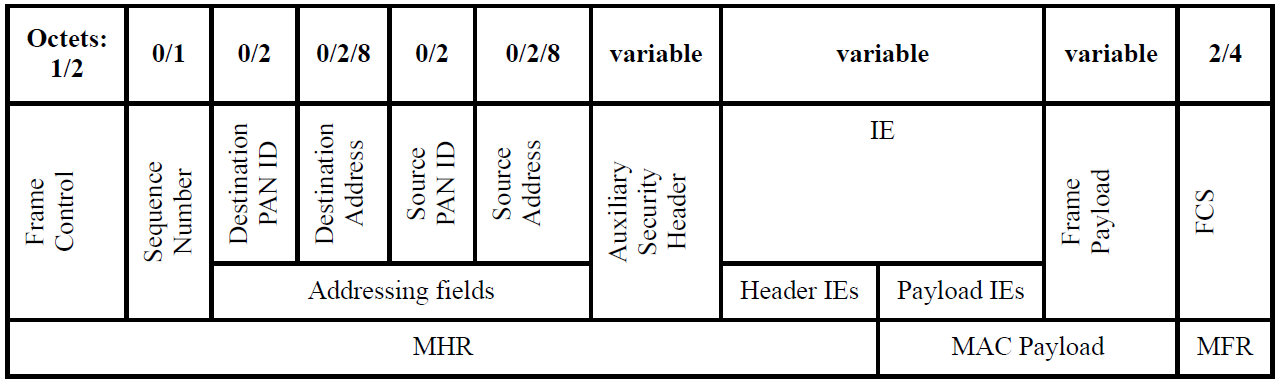
\includegraphics[width=\linewidth]{graphics/general_MAC_Frame_Format.png}
	\caption{General MAC Frame Format \cite{IEEE4-2020-7}}
	\label{f:MAC Frame Format}
\end{figure}


\subsubsection{MAC Frame Format}

Figure \ref{f:MAC Frame Format} shows the composition of a UWB-MAC frame.

In the MAC header (MHR), the Frame Control Field includes information about:

\begin{itemize}
  \item the frame-type
  \item if the Auxiliary Security Header Field is used and in what capacity
  \item if additional frames will follow
  \item if an acknowledgment message is expected
  \item if the message is between different PAN-Networks.
  \item of what type the receiver is (PAN coordinator, device, PAN-Network)
  \item the used frame-format standard
  \item where to find the source address
\end{itemize}

The Sequence Number counts up, helping to keep track of the order in which frames arive.
The Adressing Fields carry the IDs of sender and recipient for the frame.
The Auxiliary Security Header Field only exists if it was specified in the control Field.
It contains additional information needed for the chosen security methode.

There are two parts to the information element (IE).
The header IE specifies additional information about the frame, for example data formating information or chanel time allocation.
The the payload IE specifies the length and data-type of the payload field.
The payload containes the data that is sent.
It and the IE are of variable length, depending of the frame-type and data-length.

The MAC footer (MFR) marcs the end of the frame.
It only contains the frame checking sequence (FCS), that can be used to detect corrupted frames using cyclic redundancy checks.

\subsection{UWB PHY}

\subsubsection{PHY Chanel}

The IEEE 802.15.4z amendment defines 16 channels for communication for HRP UWB. 
A chanel is defined by its center frequency.
UWB devices can transmit on three different bands, high band, low band and sub-gigahertz.
For each band their is one chanel that is mandatory to support, if a device suports the band.
The other channels are optional, but if two devices want to communicate with each other they need to use the same band.
The bands, 16 chanels and their ranges and which chanels are mandatory can be found in table  (see table \ref{Table:: UWB frequency and channel assignments}).


\begin{table}[ht!]
\centering
\begin{tabular}{|l|l|c|c|}
\hline
\textbf{Channel number} & \textbf{Center frequency (MHz)} & \textbf{HRP UWB band}       & \textbf{Mandatory}  \\ 
\hline
0                       & 499.2                           & sub-gigahertz               &  \checkmark     \\ 
\hline
1                       & 3494.4                          & \multirow{4}{*}{Low band}   &                   \\ 
\cline{1-2}\cline{4-4}
2                       & 3993.6                          &                             &                   \\ 
\cline{1-2}\cline{4-4}
3                       & 4492.8                          &                             & \checkmark      \\ 
\cline{1-2}\cline{4-4}
4                       & 3993.6                          &                             &                   \\ 
\hline
5                       & 6489.6                          & \multirow{11}{*}{High band} &                 \\ 
\cline{1-2}\cline{4-4}
6                       & 6988.8                          &                             &                   \\ 
\cline{1-2}\cline{4-4}
7                       & 6489.6                          &                             &                   \\ 
\cline{1-2}\cline{4-4}
8                       & 7488                            &                             &                   \\ 
\cline{1-2}\cline{4-4}
9                       & 7987.2                          &                             & \checkmark       \\ 
\cline{1-2}\cline{4-4}
10                      & 8486.4                          &                             &                   \\ 
\cline{1-2}\cline{4-4}
11                      & 7987.2                          &                             &                   \\ 
\cline{1-2}\cline{4-4}
12                      & 8985.6                          &                             &                   \\ 
\cline{1-2}\cline{4-4}
13                      & 9484.8                          &                             &                   \\ 
\cline{1-2}\cline{4-4}
14                      & 9984                            &                             &                   \\ 
\cline{1-2}\cline{4-4}
15                      & 9484.8                          &                             &                 \\
\hline
\end{tabular}
\caption{ HRP UWB Frequency and Channel Assignments  \cite{IEEE4-2020-7, IEEE4z}}
\label{Table:: UWB frequency and channel assignments}
\end{table}

\subsubsection{Scrambled timestamp sequence}

The 4z amendment added the option to include a scrambled timestamp sequence (STS) into the frame.
The STS is a cyphered sequence that includes the timestamp and is used for ranging.
It is ment to increase the accuracy and integrtity of the raging results.
Before transmition receiver and sender exchange a randomly generated key.
The key is then used to encrypt the timestamp using the advanced encryption standard (AES) with 128 bits.
This ensured that the signal has not been intersepted and changed, to manipulate the ranging result.
Devices that support STS are called HRP-enhanced ranging capable
devices (HRP-ERDEV).

\subsubsection{Pulse Repetition Frequency}
\label{sec:pule repetition frequency}
The pulse repetition frequency (PRF) is the frequency at wich bursts are sent by the transmitter.
The mean PRF is the average PRF while sending the payload (power switching service data unit PSDU). %https://www.keysight.com/blogs/en/tech/rfmw/2021/07/28/an-overview-of-the-ieee-802154-hrp-uwb-standard
The higher the mean PRF, the shorter the airtime of each frame and allows for faster communication.
HRP-ERDEV use a different mean PRF than general devices.
They can work in Base pulse repetition frequency (BPRF) operating at mean PRF 64 MHz or in higher pulse repetition frequency (HPRF) mode operating above BPRF (Table \ref{f:mean PRF}).

\begin{table}[ht!]
\centering
\begin{tabular}{|l|l|l|} 
\hline
\textbf{Standard}          & \textbf{HRP UWB mode} & \textbf{mean PRF}            \\ 
\hline
802.15.4                   & Non HRP ERDEV         & 3.9 MHz, 15.6 MHz, 62.4 MHz  \\ 
\hline
\multirow{2}{*}{802.15.4z} & HRP-ERDEV BPRF        & 62.4 MHz                     \\ 
\cline{2-3}
                           & HRP-ERDEV HPRF        & 124.8 MHz, 249.6 MHz         \\
\hline
\end{tabular}
\caption{HRP UWB Mean PRF (Based on IEEE 802.15.4 and IEEE 802.15.4z, \cite{IEEE4-2020-7, IEEE4z})}
\label{f:mean PRF}
\end{table} %cite euse eigeni bricht

\subsubsection{Symbol Encoding}
UWB sends symbols by transmitting a burst of pulses that encode the symbol.
Since the pulses have clean edges, the arival time can be measured precisly.
This leads to the burst having two ways to carry information( \cite{QorvoGettingBacktoBasics}):
\begin{itemize}
  \item Binary phase-shift keying (BPSK: Encoding zeros and ones shifting the pulses phases so the burst beak for one has an oposite amplitude to the other. 
Figure \ref{f:UWB_signal_description} shows the singal 101 binary phase-shift keyed. 
Each bit is set twice, to detect problems with transmission.
  \item Burst position modulation (BPM): Changing the timing of the burst so it falls into a different time-slot inside of the possible burst position.	
Figure \ref{f:symbol structure} shows how the burst can be placed in a BPM-interval. 
The burst can't be placed in the guard interval. 
The guard exists to minimize inter-symbol interference from the
signals taking multiple paths.
\end{itemize}

\begin{figure}[ht!]
	\centering
	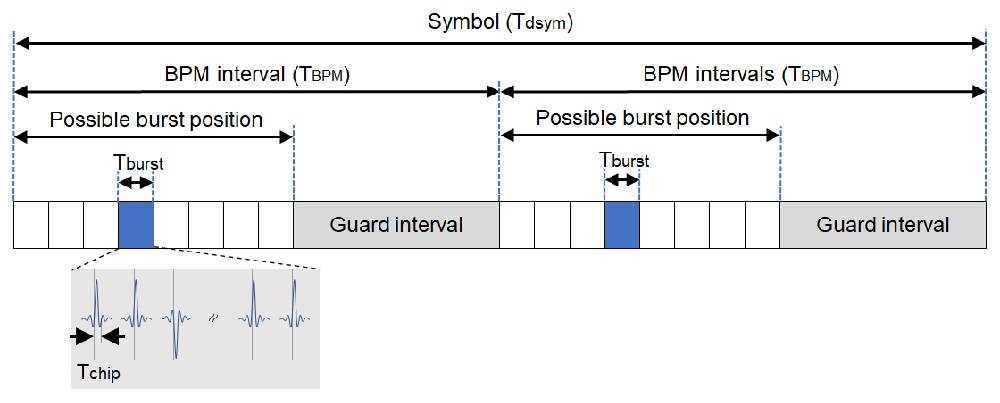
\includegraphics[width=\linewidth]{graphics/HRP_UWB_PHY_symbol_structure.jpg}
	\caption{HRP UWB PHY Symbol Structure \cite{hsu_2021}}
	\label{f:symbol structure}
\end{figure}

One or both of these encoding-strategies can be used in a uwb transmission.
The poition of the pulses inside of the burst (see figure \ref{f:UWB_signal_description})  relative to each other can be used to detect the presence of multipath effects and adjust for them. 
Using this, precises arrival times for the whole signal can be calculated.

\begin{figure}[ht!]
	\centering
	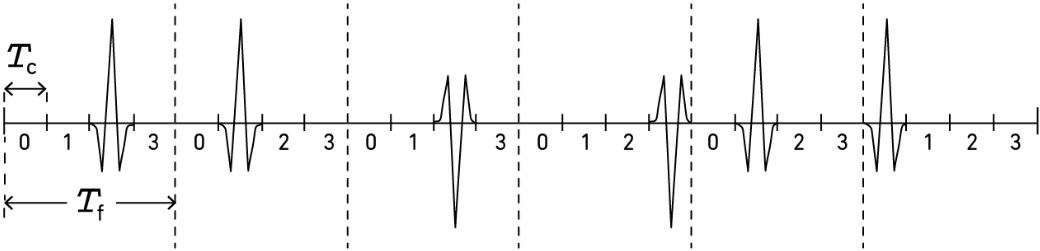
\includegraphics[width=\linewidth]{graphics/uwb_signal_tramsmission.png}
	\caption{UWB signal transmission byte encoding, \cite{QorvoGettingBacktoBasics}}
	\label{f:UWB_signal_description}
\end{figure}

Non-HRP ERDEV use BPM and BPSK.
Some HRP-ERDEV can use only BPSK, using a higher PRF and therefore reducing airtime.








\subsubsection{PHY Frame}
Figure \ref{f:PPDU general} shows a schematic view of a PHY frame as defined by the IEEE 802.15.4 standard.
The Synchronziation header (SHR) containes the information needed to detect the signal and ajust to its parameters.
The PHY header contains meta information about the payload and its encoding.
The PHY payload contains the data that is to be send, namly the MAC frame.

\begin{figure}[!ht]
\centering
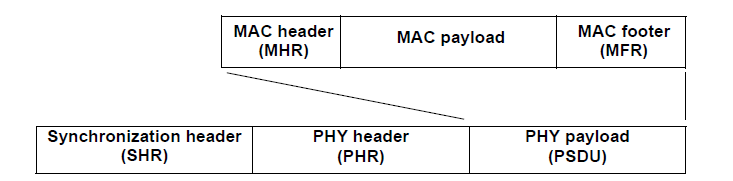
\includegraphics[width=\linewidth]{graphics/Schematic_view_PPDU.png}
\caption{Schematic view of a PHY frame defined by IEEE 802.15.4 \cite{IEEE4-2020-7}}
\label{f:PPDU general}
\end{figure}


Figure \ref{f:SHR field} shows the synchronization header, consiting of two parts.
The SYNC section is detectable by the receiver and informs it that a transmission has started.
Depending on the predefined mode, pulses of different length.
The sequence of pulses specify a set of chanels that can be used for communication.
The preamble can also be used to identify a PAN coordinator.

The SHR ends with the Start of Frame Delimiter (SFD).
It indicates that the synchronization has ended and the comming signals will be data, starting with the PHY header. 
It also contains a timestamp which can be used for ranging using time difference of arrival (ToA), see section \ref{TODO: put in this section}


\begin{figure}[!ht]
\centering
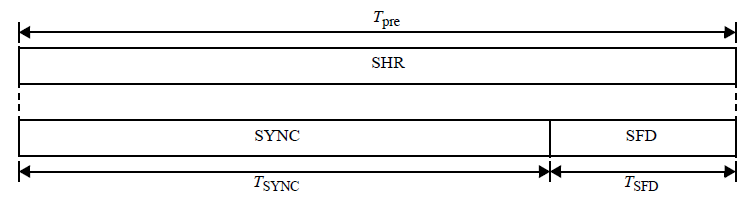
\includegraphics[width=\linewidth]{graphics/SHR_field_structure.png}
\caption{SHR Field Structure \cite{IEEE4-2020-7}}
\label{f:SHR field}
\end{figure}	

The PhY header contains all information needed to read the PHY payload (see Figure \ref{f:PHR general}).
The first bit defines the data rate that will be used during the playload transfer (see section \ref{sec:pule repetition frequency}).
The next seven bits define the length of the frame, with a frame length of maximal 128 bytes.
the 10th bit shows if ranging will be used with this frame.
The next bit is reserved.
Bits 11 and 12 define the preamble duration. It specifies how many repetitions are used, which can range from 16 to 4096.
The last 6 bits are single error correct, double error detect (SECDED) bits that form a Hammock block and can be used to correct single bit errors and detecting, but not fixing, double bit errors.

The last part of the PHY frame is the The PHY payload (PSDU).
This contains the the MAC frame, as defined in section \ref{sec:UWB MAC}.

\begin{figure}[ht!]
\centering
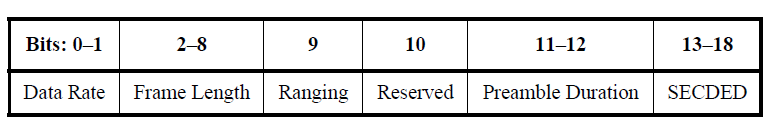
\includegraphics[width=\linewidth]{graphics/PHR_field_format_4.png}
\caption{General PHR Field Format \cite{IEEE4-2020-7}}
\label{f:PHR general}
\end{figure}

The 802.15.4z amendment contains optional changes to the PHY frame format if the participaiting devices are HRP-ERDEV devices.
Figure \ref{f:HRP-erdev frame} shows the newly allowed structures for a UWB frame.
Configuration 1 is equivalent to the already existing PHY frame.
The others additionaly contain a scrambled time stamp.
This can be placed in different places after the SHR.
Since UWB can also be used only for ranging without transmitting a message, configuration 3 only contains the SHR and STS, without a payload.

\begin{figure}[ht!]
\centering
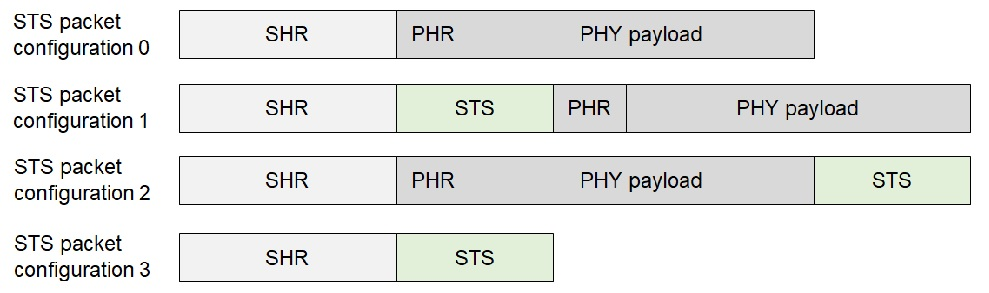
\includegraphics[width=\linewidth]{graphics/HRP_ERDEV_frame_structures.jpg}
\caption{HRP-ERDEV Frame Structures \cite{hsu_2021}}
\label{f:HRP-erdev frame}
\end{figure}

Additionally the PHR can be formatted differently (see gigure \ref{f:PHR 4z}. 
The reserved field and preamble duration is removed to make more space for the frame length. This allows to send more data in one frame, increasing the throughput of the UWB communication.

\begin{figure}[ht!]
\centering
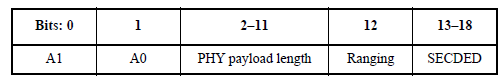
\includegraphics[width=\linewidth]{graphics/HRP_ERDEV_HPRF_mode_PHR.png}
\caption{PHR Field Format for HRP-ERDEV in HPRF Mode \cite{IEEE4z}}
\label{f:PHR 4z}
\end{figure}


\subsection{Two-way ranging}
\label{ss:two_way_ranging}
The IEEE 802.15.4z UWB standard describes two ranging methods, single-sided two-way ranging (SS-TWR) and Double-sided two-way ranging (DS-TWR).
In both instances, the distance measurement is done by calculating the time of flight (ToF) of a signal sent between two device using timestamps and multiplying it with the speed of light. 
In this section both SS-TWR and DS-TWR will be discussed.
In all other parts of the thesis,two-way ranging(TWR) refers to DS-TWR.




\section{Related Work} % application of concepts


\subsection{Artwork Tracking}


Since art preservation is an old field and temperature, humidity, light and vibrations have been known to be detrimental to most artworks, especialy paintings, most research in this direction is older than 20 years \cite{mecklenburg1991mechanical, michalski1991paintings, saunders2004effect}.
Still, the envention of new technologies, such as pattern recognizion using artificial inteligence, improvement on existing tools like infrared imaging and a active need for solutions have kept the resaech into artwork preservation an active field \cite{borg2020application, schito2017integrated}.
One such new technologies are sensor networks, which have become widespread in the field of art-preservation \cite{shah2016customized}.


Artwork tracking during transportation has not been a major focus in academia.
The most relevant related research was done by Fort et al. \cite{landi2022iot}.
They developed a low-cost, low powered sensor node to track temperature, humdity, pressure and vibrations of artwork and wooden structures.
The sensor node would then report its findings to a remote server.
They confirmed the validity of their sensor in a series of experiments, that were performed in a static building.
They also presented a theoretical framework for their sensor to be used in a transportation scenario, but they do not report having implemented or tesed this system.
Their sensor used an ascelerometer to detect vibrations, and the Bosch BME280 sensor to detect pressure, temperature and humidity.
Their sensors did not build a network and were not queried, but reported their findings directly to either a wlan router or a ble-capable smart-device.
The research of Fort et al. showed the value of low-cost sensors in the detection of threats to artwork.

\subsection{Sensor Networks}

Wireless Sensor Networks (WSN) have become a central aspect if IoT.
Researchers have tried to focus on the most prevelant problems arrising from the development of NSWs, mainly power managment, security and privacy, data integrity and avaliability \cite{gulati2022review}.


\cite{garg2021healthcare} researched WSNs outside of the controlled environment of a house. They propose a WSN that can track thevitals of mountainiers and call for help when measurements have dangerous values. 
They used an Ardruino Mega board equiped with a radio transiever, using LoRa with a star-topology, was used.


\cite{jones2021wireless} created a WSN of NRF24101 board that is intended to monitor linear infrastructures like deepsee wires, using radio and wifi for communication. Using deep sleep they were able to optimize energy usage so the sensor is predicted to last five years on batery.


\cite{spandonidis2022evaluation} used an acelerometer to detect vibrations in pipeline to discover leaks. 
They used a narrowband connection for communication and GPS for localization.
Their sensors could query each other for data, to provide a more complete image of the situation.


\subsection{Wireless ranging}

\cite{li2024indoor} made an overview of publications envolving positioning systems for industrial settings. 
They looked at the positioning systems in papers using RFID, BLE, UWB, Wi-Fi and ZigBee. They found that UWB consistently reported the highest accuracy of these methods.
UWB was the least affected by multipath-effects, although it was still the most common issue with this technology.


Early research of ranging using UWB was done by Gezici et al. \cite{gezici2008survey, gezici2005localization}.
These papers gave an overview of the different positioning systems for UWB, angle of arival, recived signal strength, time of arrival and time difference of arival.
Time of arival and time difference of arrival were studied further in these publications, presenting errorsources and mitigation tools.


Early research focused on augmentation of UWB ranging methods.
\cite{venkatesh2007nlos} proposed using integer programs for midigating the error for ranging without line-of-sight.
\cite{guvencc2007nlos} tried to solve the same issue by using methods based on the statistics of multipath-effects.
BiasSub and BiasRed was proposed to reduce the bias in time difference of arival, by appling of a well-known algebraic explicit solution for source localization  \cite{ho2012bias}.
\cite{fan2017performance} emproved uwb ranging by eliminating random error. They did this by pre-filtering, using a anti-magnetic ring to eliminate outliers and using the double-state adaptive Kalman filter to improve position accuracy.
Newer research has also begone incorporating neural networks into UWB positioning systems \cite{stahlke2020nlos, ridolfi2021uwb, che2020machine}.

UWB localization has been used in many applied context.
It has been proposed for pedestrian tracking \cite{otim2019effects}, drone flying \cite{macoir2019uwb},robot navigation \cite{zhu2020adapted}, navigation system for visualy impared people \cite{rosiak2024effectiveness} and tracking people in buildings \cite{elbaum2024investigating}.
UWB positioning systems are particularly interesting for industrial IoT settings.
\cite{barbieri2021uwb} measured the performance of three different UWB antennas, Qorvo, Sewio, and Ubisense. They measured a lot of multiplath-effects in such a complex environment. The midigated this by employing a Bayesian filtering method.
\cite{belli2024cloud} used UWB positioning in combination with Real-time kinematic positioning, to track workers while monitoring the factory. The goal was to trigger an alarm if a dangerous situation occured.

%\chapter{Design}

This section presents the principle design of the monitoring system.
In the section \ref{ss:hardware} the components used are presented.
Section \ref{Dataflow} desctibes the functionalities and responsibilities of the system components.
In Section \ref{ss:network} the network topology and data-flow is discueed

\section{Hardware}
\label{ss:hardware}

This sectiondescribes the hardware used in the project. The setup consists of two distinct components: the artwork-tags, of which there are four, and one Phone that provides the interface to the user. The tag itself consists of 4 components:
\begin{enumerate}
	\item nRF52840 Microcontroler
	\item DWM3000 UWB Shield
	\item DHT22 temperature and humidity sensor
	\item MPU6050 accelerometer and gyroscope
\end{enumerate}

\subsection{Microcontroler}
The fundament of the artwork-tag is build by the nRF52840 DK microcontroller developed by Nordic Semiconductors. 
It is part of the nRF52 series of microcontrollers intended for development.
The nRF52840 DF is specialiezed for ble communication, for which it already includes the neccesary components.
It is compatible with the nRF52 Software Development Kit (SDK), also developed by Nordic Semiconductors.
The SDK makes it possible to use the ble functionalaties and to control the pins. It aslo includes implementations for a plethera of pin based protocols.
It contains 58 pins, 48 of which are data-pins and manage the power suply for additional modules, which includes 3.5 and 5 Volt supply pins.
32 of the pins are installed in the same way as the pins on the Ardruino uno, making it compatible with many peripherals that were designed with this common board in mind, such as the dwm3000.
The remaining ten pins are enough to attach the sensors to.
The nRF52840 DK includes a USB-B port that is used for Powersuply. Additionally it is connected to two pins and is used for UART-communication and for debugging.
The nRF52 was chosen since it was avaliable and previous projects have been done with it in compination with the DWM3000 shield.
As a result a lot of initial setup was already avaliable.

\subsection{UWB shield}
For communication between the tags as well as distance measurement the DWM3000 UWB-shield developed by Qorvo was chosen.
The DWM3000 is a commonly used device for research involving UWB \cite{coppens2022overview, leu2022ghost, stocker2022performance}.
It allows low level access, but includes an SDK written in C that makes a lot of the processes transparent to the user, if they wish.
The SDK uses the Serial Peripheral Interface (SPI) for communication between the shield and the microcontroler.



\subsection{Humidity and temperature sensor}

For humidity and temperature sensors I decided to use the DHT22(AM2302) produced by Guangzhou Aosong Electronic Co. \cite{AM2302}. 
It is a comonly used sensor in IoT monitoring systems \cite{ahmad2021evaluation}. 
The vendor claims a temperature range from -40\degree to 80\degree Celsius with a precision of 0.5\degree. 
\cite{ahmad2021evaluation} could experimentaly confirm that errors did not exceed 0.1\degree Celsius. 
They also concluded that the sensor is slow in detecting temperature change. 
This is also confrimed by the user manual \cite{AM2302}, that states a read-interval of less than 2s is not possible. 

The humidity sensor can detect the full range from 0\% to 99.9\% humidity, with an advertised maximum error of 2 percent-points \cite{AM2302}.
I could not find any research that confirmed or denied these claims.

The DHT22 sensor uses three pins from the microcontroler, two pins for power suply and ground and one for single-bus communication.
Since no SDK for this type of communication has been build for the nRF52 board series, it had to be implemented manually by reading the high and low voltage on the communication pin and, detecting headers and footers and parsing the binary messages. 
Dmitry Sysoletin published a project on github (\url{https://github.com/DSysoletin/nRF52_DHT11_example}) that handles the communication between an nRF52840 and a DHT11 sensor. 
Since the communications is mostly the same, I used his implementation, but changed the parsing of the actual data to fit the encoding used by the DHT22.

\subsection{Accelerometer and Gyroscope}
The MPU6050 sensor produced by InvenSense Incorporated provides accelerometer and gyroscope data.
The accelerometer reports the acceleration in the three cardinal directions in meters per second.
The Gyroscope reports the rotation around the threee euclidean axis in degrees per second.
In this project the accelermoterdata was not used, just the gyroscope.

The MPU6050 uses 4 pins, two for power suply and ground and two communication.
The Sensor communicates using the I2C protocoll, a serial synchronus communication system.
The microcontroller acts as the master and would in theory suport multiple workers on the same bus. 
Here only the MPU6050 uses I2C and is therefore the only worker.
While the nRF52 SDK does not supply a I2C API, it offers a Two Wire Interface (TWI) implementation that is compatible with the I2C protocoll.
It even used to offer MPU6050 specific support in the older SDK. 
I was able to port this older code to the current SDK.

\subsection{Tag technical plan}
The microcontroler builds the base of the Artwork-Tag. 
The other devices are attached to it over the avaliable pins.
In the nRF52 SDK each data pin is assigned an integer value. 
These often correspon with the name of the pin according to the nRF52830 DK manual, but not always.
I will use the names given in the manual to describe the pins.
Pins are the methods by which a microcontroller controls its peripheras.

Some pins are intended for power supply.
On the NRF52840 these pins are located in section P1, see table \ref{table:ArdruinoPins}.
The three VDD pins suply electricity with a Voltage of 3.5 Volts.
A secondary power supply that uses 5 Volts is also avaliable.
What voltage is needed depends on the periipheral.
In this case, the DHT22 runs on 3.5 Volts, while the MPU6050 is made for 5 Volts.
The P1 section also contains two ground pins, that need to be connected to the peripherals and a reset pin, so restart the microcontroler.
The last pin is not connected (N.C.).
There are additional ground pins in sections P4 and P24 of the board.

The other pins are called data pins.
By using voltage modulation these pins can transfer data and therefore be used for communication.
The nRF52840 has a I/O voltage of 3.3 Volt.
This means that a voltage of 3.3 Volt corresponds to a \textit{Logic high} and 0 Volts represents a \textit{Logic low}.
This allows the data pin to transfer communication in a binary encoding.
How a signal is interpreted is defined by the used communication protocol.
The MPU6050 for example uses the I2C protocol and uses 2 datapins.
This defines that one pin is used for a serial clock and the other pin transmits data.
For the data transmission the protocol defines what a package looks like.
This includes the start condition, the voltage characteristics that signal the beginning of a package, adressing, data encoding, acknowledgments and stop condition.

The DHT22 sensor does not use a given communication-protocol.
It uses one data-pin to report its sensor data.
How that data is encoded to high and low voltage is specified in the user manual \cite{AM2302} and has to implemented manualy.

The DWM3000 shield is mounted on the 32 pins ment for arduino one connections. 
All pins are forwarded and can be used by other devices, in a common ardruino-stackable style.
If they are data-pins they will share the data.
Table \ref{table:ArdruinoPins} shows which devices use which pins.
The only pin shared by multiple devices are power and ground pins.
The microcontroler suplies enough power to support this.

The sensors are attached to the same powersource and ground as the shield, but use different data-pins.
The DWM3000 leaves enough pins unused that both sensors could be attached to them.
Since it is not visible which pins the shield leaves free, I decided to use data-pins that are not attached to the DWM3000 in any way.
Table \ref{table:otherPins} shows how the sensors are connected to the remaining open pins.

\begin{table}[]
	\centering
	\begin{tabular}{l|l|l|l|l|}
		& Pin & \rotatebox{90}{DWM3000\phantom{.}} & \rotatebox{90}{DHT22}  & \rotatebox{90}{MPU6050\phantom{.}}   \\
		\hline \multicolumn{1}{|l|}{\multirow{10}{*}{\rotatebox{90}{P4}}}
		& P1.10  & \checkmark    &             &             \\
		\multicolumn{1}{|l|}{} & P1.11  & \checkmark    &             &             \\
		\multicolumn{1}{|l|}{} & P1.12  & \checkmark    &             &             \\
		\multicolumn{1}{|l|}{} & P1.13  & \checkmark    &             &             \\
		\multicolumn{1}{|l|}{} & P1.14  & \checkmark    &             &             \\
		\multicolumn{1}{|l|}{} & P1.15  & \checkmark    &             &             \\
		\multicolumn{1}{|l|}{} & GND    & \checkmark    &             &             \\
		\multicolumn{1}{|l|}{} & P0.02  &               &             &             \\
		\multicolumn{1}{|l|}{} & P0.26  & \checkmark    &             &             \\
		\multicolumn{1}{|l|}{} & P0.27  &               &             &             \\
		\hline \multicolumn{1}{|l|}{\multirow{8}{*}{\rotatebox{90}{P3}}}
		& P1.01  & \checkmark    &             &             \\
		\multicolumn{1}{|l|}{} & P1.02  & \checkmark    &             &             \\
		\multicolumn{1}{|l|}{} & P1.03  & \checkmark    &             &             \\
		\multicolumn{1}{|l|}{} & P1.04  & \checkmark    &             &             \\
		\multicolumn{1}{|l|}{} & P1.05  & \checkmark    &             &             \\
		\multicolumn{1}{|l|}{} & P1.06  & \checkmark    &             &             \\
		\multicolumn{1}{|l|}{} & P1.07  & \checkmark    &             &             \\
		\multicolumn{1}{|l|}{} & P1.08  & \checkmark    &             &             \\
		\multicolumn{1}{|l|}{} & P1.10  & \checkmark    &             &             \\
		\hline \multicolumn{1}{|l|}{\multirow{8}{*}{\rotatebox{90}{P1}}}
		& VDD    &               &             &             \\
		\multicolumn{1}{|l|}{} & VDD    &               &             &             \\
		\multicolumn{1}{|l|}{} & RESET  &               &             &             \\
		\multicolumn{1}{|l|}{} & VDD    & \checkmark    & \checkmark  &             \\
		\multicolumn{1}{|l|}{} & 5V     & \checkmark    &             & \checkmark  \\
		\multicolumn{1}{|l|}{} & GND    & \checkmark    & \checkmark  & \checkmark  \\
		\multicolumn{1}{|l|}{} & GND    & \checkmark    &             &             \\
		\multicolumn{1}{|l|}{} & N.C.   &               &             &             \\
		\hline \multicolumn{1}{|l|}{\multirow{6}{*}{\rotatebox{90}{P2}}}
		& P0.03  & \checkmark    &             &             \\
		\multicolumn{1}{|l|}{} & P0.04  & \checkmark    &             &             \\
		\multicolumn{1}{|l|}{} & P0.28  &               &             &             \\
		\multicolumn{1}{|l|}{} & P0.29  &               &             &             \\
		\multicolumn{1}{|l|}{} & P0.30  &               &             &             \\
		\multicolumn{1}{|l|}{} & P0.31  &               &             &             \\
		\hline 
	\end{tabular}
\caption{Adruino compatible pin assignment}
\label{table:ArdruinoPins}
\end{table}

\begin{table}[]
	\centering
	\begin{tabular}{l|l|l|l|l|}
		& Pin & \rotatebox{90}{DWM3000\phantom{.}} & \rotatebox{90}{DHT22}  & \rotatebox{90}{MPU6050\phantom{.}}   \\
		\hline \multicolumn{1}{|l|}{\multirow{8}{*}{\rotatebox{90}{P6}}} 
		& P0.00  &               &             &             \\
		\multicolumn{1}{|l|}{} & P0.01  &               &             &             \\
		\multicolumn{1}{|l|}{} & P0.05  &               &             &             \\
		\multicolumn{1}{|l|}{} & P0.06  &               &             &             \\
		\multicolumn{1}{|l|}{} & P0.07  &               &             &             \\
		\multicolumn{1}{|l|}{} & P0.08  &               &             &             \\
		\multicolumn{1}{|l|}{} & P0.09  &               &             &             \\
		\multicolumn{1}{|l|}{} & P0.10  &               &             &             \\
		\hline \multicolumn{1}{|l|}{\multirow{18}{*}{\rotatebox{90}{P24}}} 
		& P0.11  &               &             & \checkmark  \\
		\multicolumn{1}{|l|}{} & P0.12  &               &             & \checkmark  \\
		\multicolumn{1}{|l|}{} & P0.13  &               & \checkmark  &             \\
		\multicolumn{1}{|l|}{} & P0.14  &               &             &             \\
		\multicolumn{1}{|l|}{} & P0.15  &               &             &             \\
		\multicolumn{1}{|l|}{} & P0.16  &               &             &             \\
		\multicolumn{1}{|l|}{} & P0.17  &               &             &             \\
		\multicolumn{1}{|l|}{} & P0.18  &               &             &             \\
		\multicolumn{1}{|l|}{} & P0.19  &               &             &             \\
		\multicolumn{1}{|l|}{} & P0.20  &               &             &             \\
		\multicolumn{1}{|l|}{} & P0.21  &               &             &             \\
		\multicolumn{1}{|l|}{} & P0.22  &               &             &             \\
		\multicolumn{1}{|l|}{} & P0.23  &               &             &             \\
		\multicolumn{1}{|l|}{} & P0.24  &               &             &             \\
		\multicolumn{1}{|l|}{} & P0.25  &               &             &             \\
		\multicolumn{1}{|l|}{} & P1.00  &               &             &             \\
		\multicolumn{1}{|l|}{} & P1.09  &               &             &             \\
		\multicolumn{1}{|l|}{} & GND    &               &             &             \\
		\hline
	\end{tabular}
\caption{Non-Adruino compatible pin assignment}
\label{table:otherPins}
\end{table}


\section{Architecture}
\label{ss:dataflow}

In order to discuss how the dataflow works, first the section \ref{ss:responsibility} will establish what services are implemented in each part of the system.
The section \ref{ss:dataflow} will explain what triggers events and how they are handled inside the system.

\subsection{Responsibilities}
\label{ss:responsibility}
The system consists of the tags, the sensor network and the phone.
These parts all have their own responsibilities.

\textbf{Tag:} 
The tag is responsible to manage its sensors. 
It has to do correct setup and converts its output into a understanable form.
The tag can performe ranging with all its neighbours.
Additionaly the tags are responsible to search for networks to join, and react aprobiatly to network request, be those queries for sensor data, ranging requests or network managment jobs. 
The tags provide a unique, secure universal identifier, to be used by queries or the network.
How this is done is part of the certify project and will not be discussed in this thesis.
The tag is also responsible for its own power managment.
This is not the focus of this thesis and will only be mentioned when relevant.
A guideline on powermanagment will not be provided here.

\textbf{Network:} The network is responsible to keep track of all tags taking part in the network. 
It offers a joining protocol for new devices and remains stable when devices leave or become unavaliable. 
It offers the possibility for phones to connect to the network. 
It ensures quieries from phones get transported to the correct tag and the answers to the correct phone.
It ensures a network topology that corresponds to a graph that is at least 3-connected.
On request it returns a list of connected devices to the phone.

\textbf{Phone:} The phone connects to the network via the provided method.
It offers a graphical user interface (GUI) to be used by the driver.
The GUI offers a method for the driver to set the acceptable ranges for all sensor data.
Additionaly it offers a method to set query intervals-length.
The phone is responsible to query sensor data for each tag and masurement once in each interval.
The phone has to evaluate the answer.
The phone has to report the results to the driver using the GUI.
If a parameter falls outside of the acceptable range for its type, the phone is responsible to alert the driver to this fact.

The certify project also plannes to collect the sensor data on remote servers using a 4G connection.
The plan is to equip each tag with antennas to allow it to send the data directly to the server itself.
Since this is not a part of this thesis, the responsibility for the tag to do this was not added to a list.
A known problem with this plan is, that a 4G connection is not always possible.
Since small tags have very limited memory, the plan to store the sensor data on the tag is not pheasible.
If the setup presented in this thesis is used, it would allow for the storage of the data on the phone, which has a much larger memory.
This again was not added, since it is not part of this thesis.

\subsection{Dataflow}
\label{ss:dataflow}

\begin{figure}[ht!]
	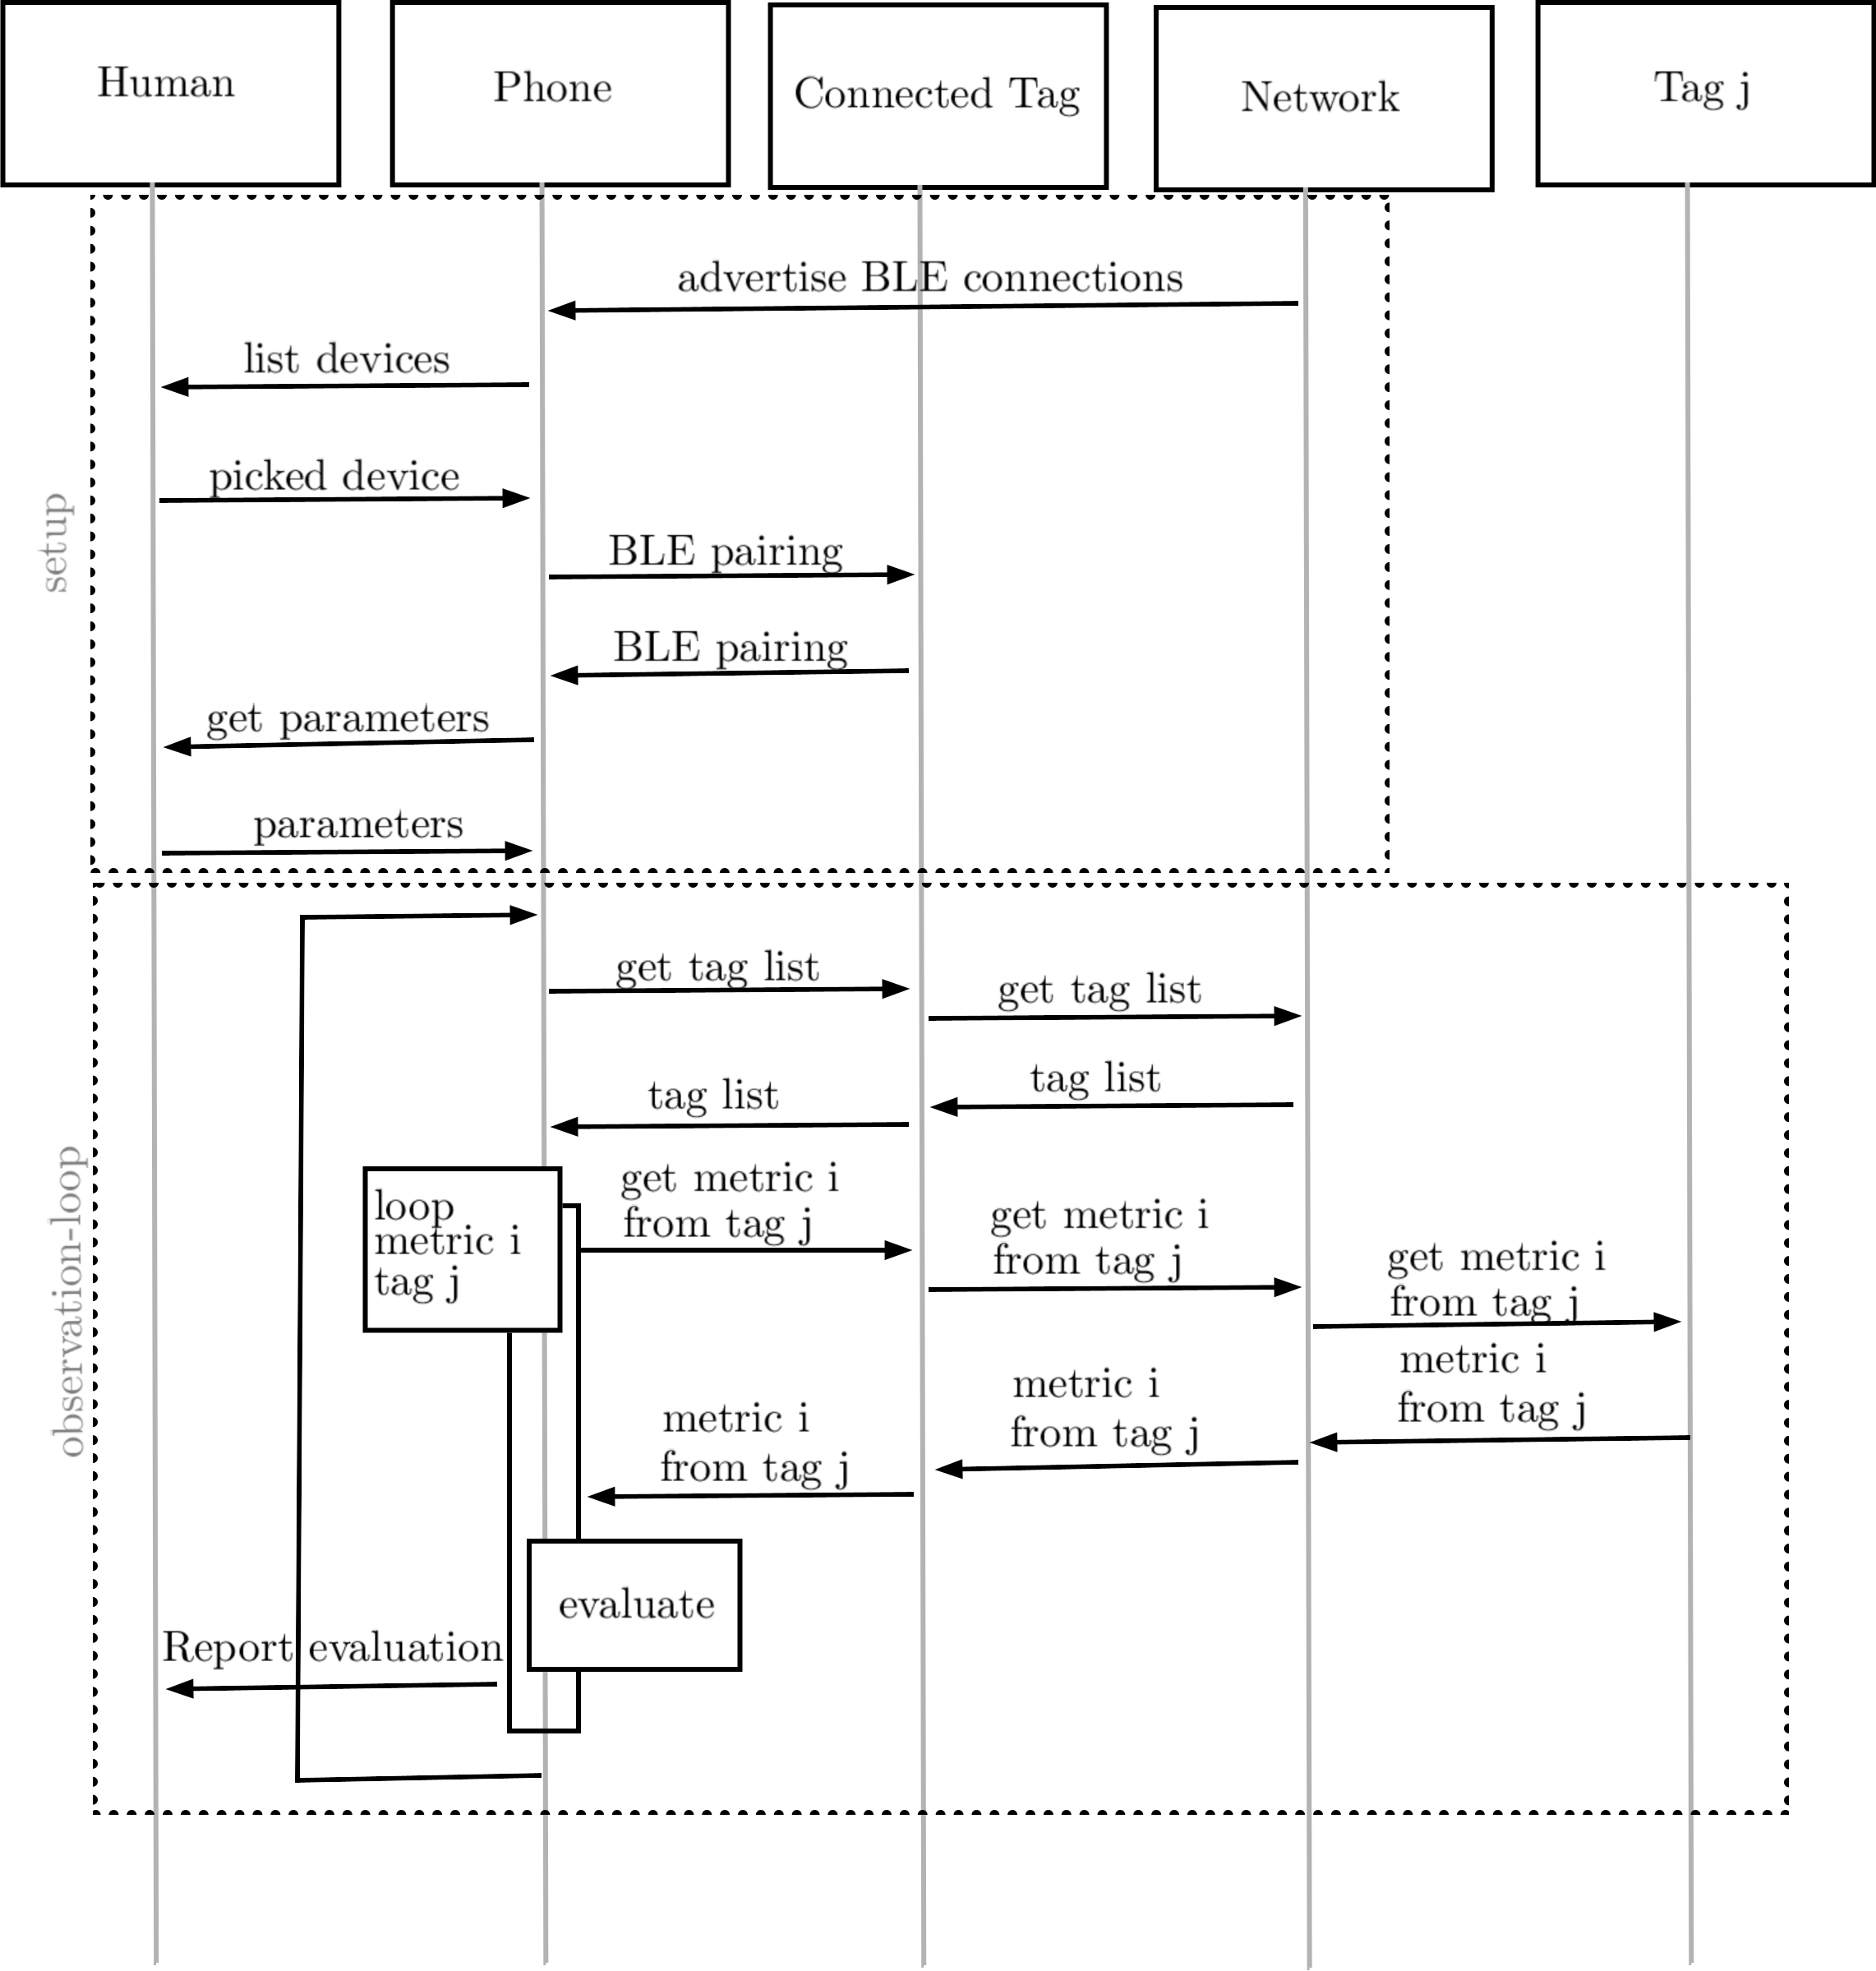
\includegraphics[width=\linewidth]{graphics/schematics/obervation_loop.png}
	\caption{Sequence diagram of setup and oberservation loop. Setup is performed once, oberservation loop repeats until stopped.}
	\label{f:observation_loop}
\end{figure}

How a tag connects to the network is described in the section \ref{s:network}.
Figure \ref{f:observation_loop} shows a sequece diagram ob the setup and main observation loop of the system.
On the top the communicating parts are listed.
\begin{itemize}
	\item Human is the driver of the truck
	\item Phone is the phone used by the Human
	\item Network consists of all the tags that are used and the network they build.
	\item Connected Tag is part of this network, but is listed seperatly. It represents the tag that is communicating to the phone
	\item Tag j is also part of the Netowrk. It represents the tag that is queried during the observation loop
\end{itemize}
Phone and Human communicate by using a GUI. Phone and Connected Tag commuincate using BLE. Every communication inside the network happens using UWB. This includes the communication between the Connected Tag, the network and Tag j. \\
When the phone wants to connect to the network, it looks for advertised BLE devices.
It then displays the devices to the user and lets him pick one.
The phone then pairs to the chosen tag, making it the connected tag and the phones connection to the network of tags.
Once connected to the network, the phone will promt the human to enter the parameters.
These consist of:
\begin{itemize}
	\item Upper and lower limit for sensor data, like temperature and humidity
	\item Maximal displacement value for distance and gyro. These values represent the maximal difference in registered values that is allowed for positional measurements.
	\item Time between measurements. This gives the time period that will pass between measurements for each device and measurement type.
\end{itemize}
Once the parameters chosen, the user can start the observation.\\
Each iteration of the observation loop begins with a call to the network for a list of all tags currently in the network.
Since the tag network is a dynamic sensor network, the tags in the network can theoretically change. 
In practice this should onyl happen, when artwork is unloaded or if a tag becomes faulty.
The request for the list is transmitted to the connected tag ober BLE, which than queries the network for all conected devices.
The responde is returned to the Phone.
The phone then starts a nested loop, iterating over the list of tags and the list of metrics caputred by the system.
For each measurement and tag combination (i,j) the phone contacts the connected tag for the value, which in turn queries the network.
Once the message has arrived at the tag j, tag j gets measurement i. In case of sensors this intails contacting the sensor and requesting a value.
If metric i is a distance measurement, tag j will commence a two-way ranging operation over UWB with all its registered neighbours and will report the list of distances, together with the tag-adresses they correspond to.
Metric i is then transported over the network back to the connected tag and finaly to the phone.
The phone must then evaluate the retrieved data. \\
During the evaluation process, the phone creates an evaluated measurement, and marks it as problematic or unproblematic.
What the evaluation looks like depends on the metric.
\begin{itemize}
	\item For most metrics, like humidity and temperature, the evaluated measurement is equivalent to the received measurement. It is then checked, if the measurement falls into the aceptable measurement parameters, set by the human.
	If it does not, the evaluated value is marked as problematic.
	\item Some metrics require comparisment to the previous data. The gyroscope reports the current orientation of the tag.
	This is then compared to all previous measurements and the maximal angular difference forms the evaluated measurement.
	If the evaluated metric is bigger then allowed by the set parameters, the measurement is marked as problematic
	After evaluation the original measurement is added to the list of previous measurements.
	\item The distance measurement has a unique evaluation process, which is describbed in section \ref{ss:distance_eval}.
\end{itemize}
Once the data evaluation is done, the evaluated measurement is presented to the user over the GUI, together with the adress of the tag it belongs to.
If the evaluated measurement is problematic, the driver it alarmed.


\subsubsection{Distance evaluation}
\label{ss:distance_eval}
The goal of the distance evaluation is to build a working model of where every tag is.
To achieve this, a quadratic program is solved, to get the coordinates of all tags.
The steps to do this are as follows:
\begin{enumerate}
	\item Get a list of all current tags, $T:=\{ t_1, t_2, ... \}$.
	\item For each tag, get the last known distance measurements and put it into a set $S_D:=\{ (t_i, t_j, d_{ij}) \} $, where $t_i$ is the tag which measured, $t_2$ the tag that was measured to and $d_{ij}$ the distance measured.
	\item If a tag has no distance measurements, remove it from the list.
	\item Assign each tag $t_i$ a position in a 3D coordinate system, $(x_i,y_i,z_i)$
	\item Pick one random tag $t_{o}$.
	\item Set the values $x_{o},y_{o},z_{o}$ all to 0.
	\item Create the objective function: $L(X,Y,Z) = \sum\limits_{t_i, t_j, d_{ij} \in S_D}|(x_i-x_j)^2+(y_i-y_j)^2+(z_i-z_j)^2-d_{ij}^2|$. For x,y and z use variables for all but the six values set in step (6).
	\item Solve the quadratic program consting of the Objective function L and no constrains.
\end{enumerate}
Quadratic Programs in general are NP-Hard, but Quadratic Programs with a convex function can be solved efficiently.
$(a-b)^2$ and $c$ are convex functions.
The sum uf a convex function is always a convex function.
The objective function in (7) only sums up convex functions and is therefore convex itself.
The quadratic program can therefore be solved efficiently.\\
By setting the values of tag $t_{o}$ to zero, the results of the quadratc function becomes grounded.
It is not strictily nessecary, but without it the returned solution could have values anywhere in the Euclidean space.
by setting one tag to the coordinates at theo origin, the solution will place the other tags near that region.
There are still an infinte amount of solutions to this quadratic function, since all solutions can be roatated around any axis and still return the same objective function.

\begin{figure}[ht!]
	\begin{subfigure}{.4\linewidth}
		\centering
		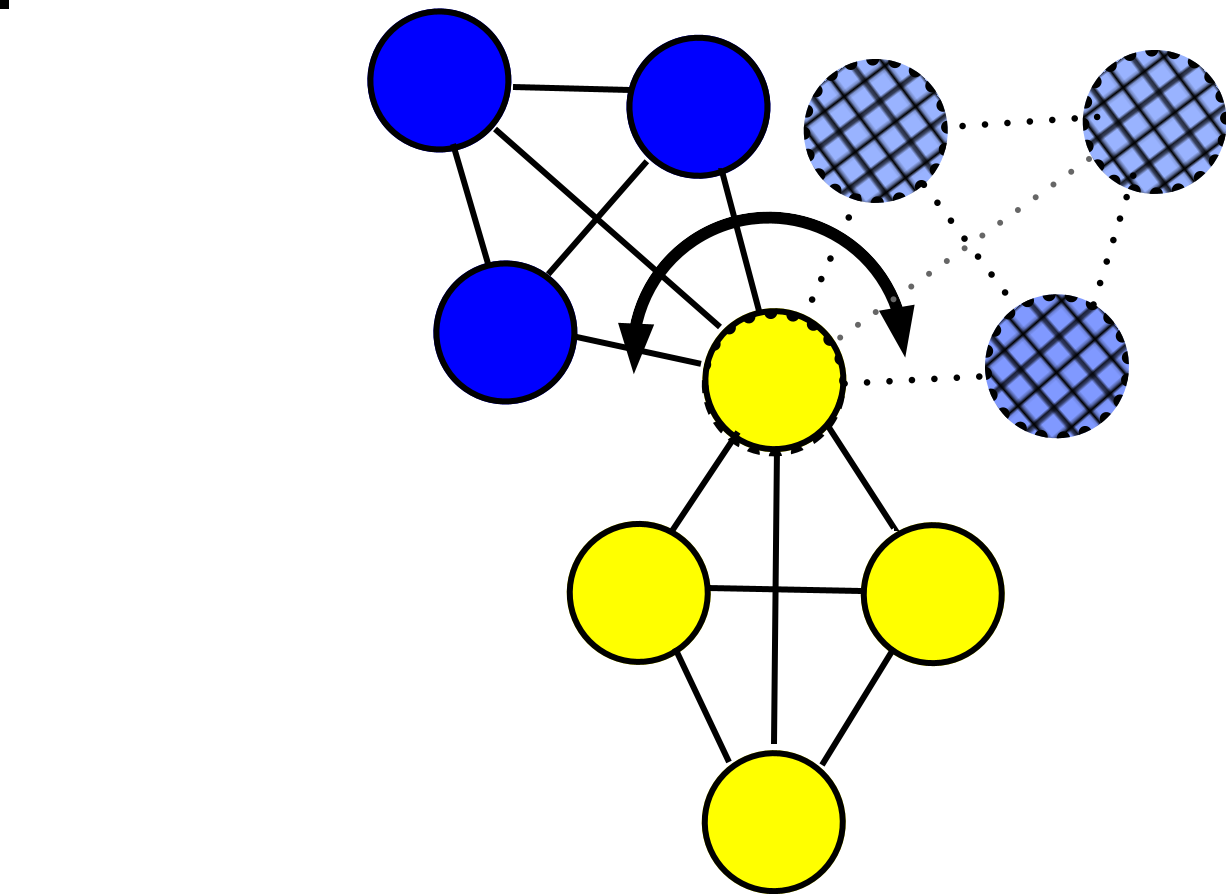
\includegraphics[height=150px]{graphics/schematics/connected_dots.png}
		\caption{3-edge connected graph}
	\end{subfigure}
\hspace{1cm}
	\begin{subfigure}{.4\linewidth}
		\centering
		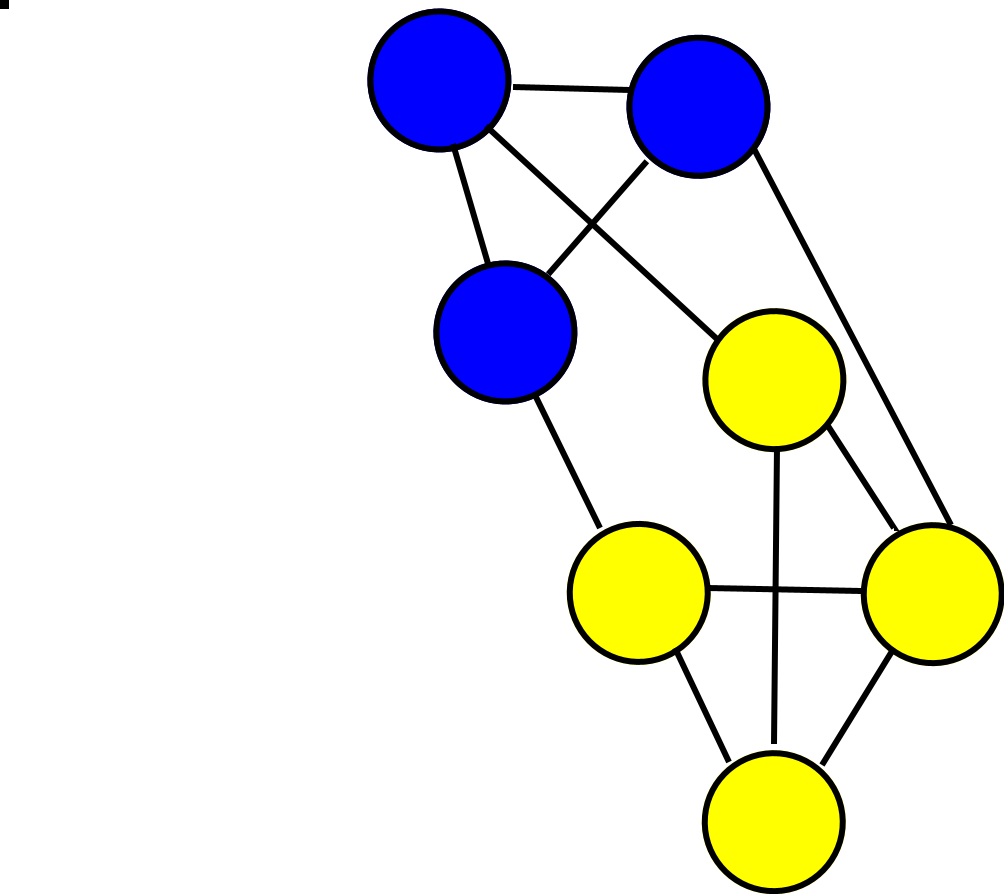
\includegraphics[height=150px]{graphics/schematics/connected_dots_k_connected.png}
		\caption{2 connected graph}
	\end{subfigure}
	\caption{ Left: Five dots, all having at least two connections, still blue can move independently. Right: minimal 2-connected graph, no movement possible. }
	\label{f:connected_dots}
\end{figure}

For a point to be clearly placed in Euclidean space, three distances to other points have to known.
This alone is not sufficient to insure a unique results.
The left of Figure \ref{f:connected_dots} illustrates this point in two-dimensional space.
Every circle is connected to two others, still the blue circles can move without the whole figure moving.
What is needed to keep every point static is for known distances and tags to build a four-connected graph (three in two dimensions).
The left of Figure \ref{f:connected_dots} shows a sollution of the problem on the right by creating a three-connected subgraph.

Once the coordinates for all tags are found, they are compared to previous results.
For each tag the phone calculate by how much it has moved.
The evaluated measurment is the distance of the tag that has moved the most.
If the evaluated measurement is larger then the maximal allowed displacement, the measurement is problematic.



\section{Network}
\label{s:network}

For the presented network to work, tags need to be ranked.
This means that for each tag pair $i,j$, one can either say that $rank(i)<rank(j)$ or $rank(j)<rank(i)$.
To achieve this, the universal unique identifiers are used.
No matter what form the UUID has, it can be converted to an integer, by simply interpreting its binary code as one.
Since the UUIDs are unique, no to tags will have the same resulting integer.
When refering to the rank of a tag in this section, the integer representing the UUID is intended.

The tags inside the truck, while not connected to a phone, form a dicentralized mesh using UWB for communication.
Each tag keeps two list, a list of known devices and a list of neighbours.
When a new tag joins the network, it sends a joining request over UWB, containing its universal unique id (UUID), using a weak signal.
All tags in the network that receive this request add the new device to their list if known devices. 
If the new devices also has a heigher rank, they additionaly add it to their list of neighbours.
They then answer by sending their own UUID and adress back to the new tag.
By waiting an amount of time that correlates with their UUID, the tags in the network can ensure, that their answers don't overlap.
The new tag adds the received adresses and UUIDs to its known device list. If the rank of the added tag is also has a higher rank then the new tag, it will add it to the list of neighbours.
If the new tag now has four neighbours, it stops. Otherwise it will repeat the process with a incresasingly stronger signal, until it has either found four tags with higher rank or reached maximum signal strength.
Afterwards it starts addvertising its BLE connection.
This concludes the network joining process.


A user with a phone can connect to any of the advertised BLE connection.
Once that happens, the tags in the tracks will switch from their dicentralized mesh to a star-topology, with the connected device serving as the coordinator.
The coordinator will inform all tags about its new status, by sending a message using a strong UWB signal.
The tags will then acknowledge this message in order of rank.
The tags in the network will still keep their stored neighbours and known devices.
The coordinator records a list of all acknowledgemtns, thus creating a list of all devices in the network.


The phone can request the list of all tags from the coordinator.
The phone can now also query the tags in the truck by sending the query to the coordinator over BLE, which then will pass it directly to the apropriate tag using BLE.
For all sensor data, this is a simple call and response request. \\
If a distance measurement is queried, the tags takes the following steps:
\begin{itemize}
	\item It conducts a UWB two-way ranging session with each tag in the neighbour list.
	\item It reports those results to the coordinator tag.
	\item It orders all received distances.
	\item It keeps the tags with the four lowest distances and deletes the rest from the neighbour list.
\end{itemize}
The first time a distance is requested, the tag will perform more ranging sessions then necesary to build a 4-connected graph.
Afterwards it only perform ranging with four other tags, unless a new device was added.
If a ranging session does not report a result, because a tag left or became unavaliable, the tag adds ads the tag with the shortest previously measured distance and higher rank from the list of known devices back intro the list of neighbours.


This design mirrors the algorithm proposed by \cite[khan2007simple] and presented in section \ref{ss:k_connected_explained}.
It creates an approximation of a minimaly weighted k-connected subgraph, based on the measured distances.
This is allowed, since the distances are in euclydean space, which when mapped to a graph forms a metric graph.
As discussed in section \label{ss:distance_eval}, a four-connected graph is needed to uniquly identify the position of each tag.
The graph should be minimaly weighted, so that measurements are between tags that are as close as possible to each other.
This reduces the multipath effect and theirfore increases precision.


If the tags are not connected to a phone and report their data to a remote server, they can still use the same distance-measurement, to approximate the k-connected subgraph.
The quadratic program can then be calculated on the server.
%\chapter{Implementation}
\label{c:implementation}

In this section, the implementation that was used for the experiment is discussed.
In section \ref{s:tag} the implementation of the tags is presented.
Section \ref{s:app} shows the implementation of the App.

\section{Tag}
\label{s:tag}
The software of the tags consits of n modules:
\begin{enumerate}
	\item Temperature and humidity sensor
	\item Gyroscope
	\item UWB network
	\item Two way ranging
	\item BLE communication
	\item Job handler
\end{enumerate}
The following subsections will discuss the first five modules, followed by how they interact using the job handler module.
The section \ref{ss:combination} discusses chalanges from combining these modules and how they were solved.

\subsection{Temperature and humidity module}
\label{ss:temp_hum_module}
This module is responsible for managing the DHT22 humidity and temperature sensor.
It is responsible to setup the sensor during initial startup and to provide the sensors measurements when queried.
The DHT22 sensor communicates using only one data pin, pin 13, which will be referd to as the data pin in this section.
Dmitry Sysoletin created an implementation \ref{sysoletin2021nrf52_dht11} for the DHT11 sensor together with the nRF52840 board that build the basis for this implementation, by addapting it to the DHT22 and adding functionalities needed by the job handler module.


Since the DHT22 is a very simple sensor, using single bus comunication, not much setup is needed.
The evaluation of the sensor data requires that the voltage of the pin is read out in pre-defined intervals, when reading the sensor data.
To do this, a clock is required.
This resource has to be reserved an initiated at startup.
This is the only setup that is required for the DHT22 sensor.


To initiate a sensor-read the voltage of the data pin is set to 0.
When the sensor is in standby mode, the data pin is on \textit{logic high}, and when set to \textit{logic low}, the sensor will respond with a read of its current value.
A schematc view of a sensor read of the DHT22 can be seen in Figure \ref{f:dht22_signal}.
The temperature and humidity module will then check the Pin State in intervals of 5ms, until a \textit{logic low} is registered, signalling that the sensor has registered the request. 
The module will now monitor the pin state, waiting for \textit{logic low} followed by a \textit{logic high}, this beeing the start condition of the data transfer. \\
The data is transfered in five chunks of eight bits.
Each bit is preceeded by a prolonged \textit{logic low} state, that is detected by the module
The module then proceeds to write the state of the data pin into a 8-bit buffer, \textit{logic high} corresponding to a 1 and \textit{logic low} to 0.\\
Once all five chunks are read, the communication has ended and the module can verify the data.
The first two bytes correspond are combined to form the temperature information in celcius, the second and third form the humidity.
Both values are multiplied by 100 and stored in a 16-bit integer. This doesn't loose data, since the sensor only measures up to a precision of 1 after the decimal point.
The data beeing stored in an integer help with data transfer.
It will be converted back on the phone.
The fith chunk contains the parity and is used to accept or reject the humidity and temperature values.
If the process fails at any state, -100\degree C is returned for the temperature and -100% for humidity.
These form both impossible values, since humidity can't be negative and the DHT22 sensor can only detect temperatures as low as -20\degree C.


\begin{figure}[ht!]
\centering
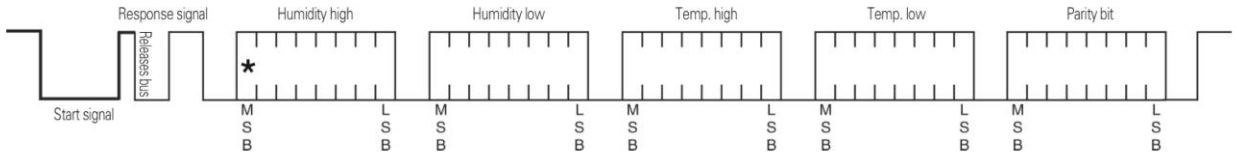
\includegraphics[width=\linewidth]{graphics/DHT22_signal.png}
\caption{Signal of a DHT22 sensor-read as presented in the manual \cite{AM2302}.}
\label{f:dht22_signal}
\end{figure}

\subsection{Gyroscope}
\label{ss:gyro_module}
This module manages the MPU6050 gyroscope and accelerometer.
It is responsible to setup the sensor and report its result.
An implementation for the MPU6050 was present in the nRF52 15.3.0 SDK, but is no longer avaliable for the nRF52 17.1.0 SDK, used in this project.
The old implementation was ported to this project.
This consisted of replacing deprecated parts of the SDK with updated ones and adding newly required flags to the build.


MPU6050 sensors use the I2C communication protocol.
The nRF52 SDK does not include an implementation for this protocol, but has a Two Wire Interface (TWI) implementation that is compatible with the I2C protocol.
During startup the TWI module has to be initialized.
This is handled by the SDK, but requires some parameters to be passed.
\begin{itemize}
	\item The Serial Clock Line (SCL) defines what pin will be used for the clock shared in the TWI. This implementation uses pin 11.
	\item The Serial Data Line (SDA) defines which pin is used for the data communication. Pin 12 was used.
	\item The frequency which the TWI uses. It is defined in MPU6050 data sheet, and is 100 kHz \cite{MPU6050}.
	\item The Interrupt priority is a rank that determins, how easyely this process can cause an interrupt. It is set to high.
\end{itemize}
After the TWI service is initiated with these parameters, it is enabled, ensuring that its resources are locked and can not be used by other services.


Afterwards the results from the sensor can be read using the TWI service again.
The TWI-TX requires the adress of the read device and a registry where to write the MPU6050 datasheet \cite{MPU6050}.
The adress of the sensor is the same for all MPU6050 sensors and can be found in the manua
It sets a flag to true once the sensor has writen the data, which then can be read using the TWO-RX function.
The result consist of three 16-bit integers, representing the angular velocity arround the X,Y and Z axis, shown in figure \ref{f:MPU6050_orientation}.\\
Returning this data when queried has only limited use.
It represents a measurement of the current situation.
The caller is more interested what happened since the last query.
Two different implementations for the read of the gyroscope were used during the experimental phase of this thesis.
One would try to return the current orientation of the tag. This read will be called the \textit{orientational read}.
The other would return the maximal registered angular velocity since the last read. This will be called the \textit{angular velocity read}.


\begin{figure}[ht!]
\centering
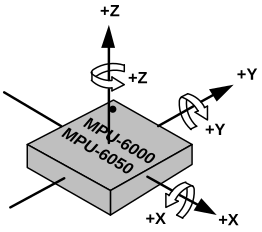
\includegraphics[width=200px]{graphics/MPU6050_orientation.png}
\caption{Schematic view of the MPU6050, showing the direction of the three axis X,Y,Z.}
\label{f:MPU6050_orientation}
\end{figure}



To achieve the orientational read, three orientational variables $x_{angle}$, $y_{angle}$ and $z_{angle}$ keep track of the current rotation around their corresponding axes.
During setup, all three angles are set to zero.
The MPU6050 is read out periodically in between calls.
The elapsed time since the last read is multiplied with the angular velocity at this moment arround the axis and is added to the orientational variables.
When the gyroscope module is queried for its measurement, $x_{angle}$, $y_{angle}$ and $z_{angle}$ are returned.


The angualr velocity read is achieved in a similar manner.
Three angular velocity variables $x_{max}$, $y_{max}$ and $z_{max}$ are created and set to zero during initiation.
The MPU6050 is read out periodically and its values are compared to the angular velocity variables.
If any of the angular velocity values is smaller in absolute magnitude than the corresponding read value, it is replaced by that read value.
When the the gyroscope module is queried, the values of $x_{max}$, $y_{max}$ and $z_{max}$ are returned.
The angular velocity variables $x_{max}$, $y_{max}$ and $z_{max}$ are then set to zero again.

\subsection{Network}
\label{s:network}
The network module is responsible for the managment of the network.
This consists of: sending requests to join a network, managing requests to join a network, keeping track of its neighbours, transmitting messages and sending messages.
Since only four devices were used in this implementation, the processes for the network are much more simplified, then presented in design chapter.
A 4-connected minial graph of 4 verteces must nececarily include that all the nodes are fully connected.
This leads to a simplified network architecture.
Since this implementation was build to run experiments and not to be used in real-world applications, a lot of security measures were canceled.
Messages are not encrypted and devices are not authenticated.
All messages are assumed to reach their destination and no devices is expected to become unavaliable. \\
The Network-module is based on the implementation of \cite{degkwitz2023ultrawideband}.
It is based on published examples from Qorvo, the producer of the DWM3000 shield.
It uses the DWS3000 SDK to communicate with the DWM3000.


The DWM3000 uses the Serial Peripheral Interface (SPI) protocol.
This requires some resources that have to be reserved and some configurations that need to be set.
This is the first thing that happens during the setup of the UWB network.
Next the interrupt-priorities and the communication speed of the SPI connection are configured.
Then the DWM3000 is reset, to insure no cross-effects from previous sessions are possible.
Then the board is told to initialize.
After that the used configurations are send to the shield.
This includes information like chanel number, preamble codes, data rates and header modes.
The SDK contains many pre-defined configurations.
All configurations that allow for RX and TX and that use scrambled timestampt (STS) work for this usecase.
It is crucal that all tags use the same configurations.
For this implementation the same configurations were used, as in \cite{degkwitz2023ultrawideband}.
The configurations can be seen in table \ref{table:DWM_settings}.
The setup finishes with initiating the LEDs, that serve no critical service, but are usefull for debugging.



\begin{figure}[ht]
\caption{Configurations of the DWM3000 for UWB communication}
\begin{longtable}{|l|c|}
\hline
\textbf{Description} & \textbf{Value} \\
\hline
\endfirsthead
\hline
\endfoot
Channel number & 5 \\
TX preamble length & 128 symbols \\
RX preamble acquisition chunk size & 8 chunks \\
TX preamble code & 9 \\
RX preamble code & 9 \\
SFD type selection & 4z 8 symbol\\
Data rate & 6.8 Mbits/s \\
PHY header mode & standard PHR mode \\
PHY header rate & standard PHR rate \\
SFD timeout & 129 \\
STS mode & enabled \\
STS length & 128 bits \\
PDOA mode & off \\
\hline
\end{longtable}
\label{table:DWM_settings}
\end{figure}


The Certify project uses unique, falsifiable identifiers for its tags.
Since this is not avaliable for the tags used here, the device-ID was used instead.
It serves as a 8-bit long adress for the purposes of this implementation.
Each tag also keeps a list of all known adresses, called neighbours.


The adress \textit{0x3F} was used, when a tag wants to join a network.
This was chosen since none of the used devixes had this device-ID, and it corresponds to a question mark when using ASCI encoding.
When a tag wants to joind a message, it sends the adress \textit{0x3F}, followed by the message 'findnet', and its own adress.
It then start listening for answers.
If the listening timed out without any answers, it sends the message again.


For the network to function, the receiving and sending of messages is critical.
The UWB listener function from project \cite{degkwitz2023ultrawideband} was modified.
It waits for a listened message from the shield.
If it receives a message, it coppies it to a buffer.
It then checks the first bit of the message for the receiver adress.
If the receiver adress is equivalent to the tags own adress, it passes the message on to the job-handler module for further evaluation.
Otherwise the message is discarded.
An exception is made, if the receiver-adress is "\textit{0x3F}", indicating that a tag is looking for a network.
In that case, the network module adds the tag to the list of neighbours.
It then waits for a time proportional to its own adress, before continuing.
Since adresses are unique, this ensures that no two tags responde to the new tag at the same time.
Afterwards it sends a new message, beginning with the adress of the new tag, followed by the string 'NEW' and its own adress.
This way it can be added to the neighbours of the new tag as well.\\
For sending messages, the implementation of \cite{degkwitz2023ultrawideband} was modified.
It sets the DWM3000 to TX, passes a int-buffer and lets it transmit, before returning to RX mode.
Do to limitations discussed in section \ref{ss:combination}, the message length could not exceed 10 bytes. 


\subsection{Two-way ranging}
\label{ss:two_way_ranging}
The two-way ranging module is responsible for measuring its distances to the tags in the neighbourhood.
Since it also uses the DWM3000 shield, it requires no additional setup.


When the two way ranging module gets a distance request, it loops over the list of neighbours, performing two-way ranging with each of them.
First it sends a prepare-rainging request to the neighbour it wants to performe ranging with, before performing the ranging.
It then sends the result back over the network to the requesting tag with the following format: 
\begin{equation}
	\mbox{$a_r$DST$a_ta_ncd_{tn}$}
\end{equation}
with
\begin{itemize}
	\item $a_r$: The adress of the requesting tag.
	\item DST: The string "DST", indicating the purpose of the message.
	\item $a_t$: The own adress of the tag performing the measurement.
	\item $a_n$: The adress of the neighbour that the distance was measured to.
	\item $c$: A boolean. If false, this is the last neighbout measured for this query.
	\item $d_{tn}$: The distance to measured. 
\end{itemize}
The reason for each measurement triggering its own response is the message-lenght limitation mentioned in section \ref{s:network}.

When a tag receives a prepare-rainging request intended for another device, it enters a short sleep.
This is because rainging envolves multiple messages beeing send netween both participants.
This would unnecesarily drain energy from the tags that are not envolved.
Because of that they sleep for the expected duration. \\
If the tag is the entended receiver for the prepare-rainging message, it will enter the preparation part of the two-way ranging module.
If will function as deivce A in respect to figure \ref{f:ds_twr_3}.
In a first step, it will clear all RX and TX buffers.
It then sets the expected RT and TX antenna delays, $d_{rx}$ and $d_{tx}$.
They represent the expected time loss during receiving or transmitting messages and are device specific.
These delays will automatically be taken into account, when calculating the timestamps.
It then sends the first polling message and imideatly starts waiting for a response.
The polling message is a constant string with no changing data.
The DWM3000 will automatically store the transmission and reception timestamps, their is no need to retreive it right away.
When the response is received, it checks if it is the expected response.
If it is, the two timestamps $T_{TX_1}^A$ and $T_{RX}^A$ are retireved.
The final transmission time $T_{TX_2}^A$ is calculated by adding a constant $c_A$ to $T_{RX}^A$:\begin{equation}
	\mbox{$T_{TX_2}^A$=}
	\mbox{$T_{RX}^A+c_A$}
\end{equation}
The final message is then prepared, containing all three timestamps $T_{TX_1}^A$, $T_{RX}^A$ and $T_{TX_2}^A$.
The message is loaded into the message buffer of the DWM3000 and a delayed transmission is started.
The delayed tranmission takes the timestamp $T_{TX_2}^A$ and will start the transmission once that timestamp is reached.
Afterwards all caches are cleaned and the tag returns to its previous state, listening for requests.

The tag that performs the ranging roccesponds to device B in figure \ref{f:ds_twr_3}.
Once it has sent the the prepare-rainging message to its neighbour, it will enter the revceiving part of the two-way ranging module.
As device A, device B will also start by settings its antenna delays $d_{rx}$ and $d_{tx}$ and clear all its RX and TX buffers.
It will then start polling for a message.
Once a message from device A is received and validated, it will retreive the timestamp when the message was received, $T_{RX_1}^B$.
Device B will add a constant $c_B$ to this timestamp to get $T_{TX}^B$:
\begin{equation}
	\mbox{$T_{TX}^B$=}
	\mbox{$T_{RX_1}^B+c_B$}
\end{equation}
It will then start a delayed transmission for the response message at $T_{TX}^B$.
The response is a constant string without any data.
Once the response is sent, device B starts to listen for messages again.
When the final message is received from device A and validated, $T_{TX_1}^A$, $T_{RX}^A$ and $T_{TX_2}^A$ are extracted from the message.
Device B also retreives its final timestamp, $T_{RX_2}^B$.
Once this is done, the time of flight for a single message can be calculated, and from that the distance:
\begin{align}
    T_{round1} &= (T_{RX}^A - T_{TX_1}^A) \\
    T_{round2} &= (T_{RX_2}^B - T_{TX}^B) \\
    T_{reply1} &= (T_{TX}^B - T_{RX_1}^B) \\
    T_{reply2} &= (T_{TX_2}^A - T_{RX}^A) \\
    ToF^{AB} &= \frac{(T_{round1}\cdot T_{round2}) - (T_{reply1}\cdot T_{reply2})}{T_{round1} + T_{round2}) + (T_{reply1} + T_{reply2}} \\
    distance &= ToF^{AB} \cdot c_{air}
\end{align}
The distance is then returned, all caches cleared and the module continues with the next distance measurent, if any are remaining.


The TX and RX antenna delay $d_{rx}$, $d_{tx}$ are different for each device.
Qorvo supplies a default value, but it is the same on all devices.
Since te antenna delays are multiplied with the speed of light, even small mistakes in calibration can lead to big errors.
According to qorvo, without the calibration of antenna delays, a measurement can be off by up to 40 cm \cite{DWM3000Calib}.
This will be a constant bias and not change over measurements.\\
Qorov has published a manual on how to calibrate their devices \cite{DWM3000Calib}.
They have not published a codebasis that implements this process.
The calibration process published by Qorvo required things that were not part of this project:
\begin{itemize}
	\item A synchronized clock, shared over all devices, without significant clockdrift
	\item A UART connection to a computer
	\item A pipeline performing statistical analysis and coordinating the devices.
\end{itemize} 
Since implementing this calibration process whould have been out of scope for this thesis, a simpler version was designed.
The tags were set up in a theathedron, so each tag was 30 cm apart from each other.
Then one tag would perform two way ranging with another tag, chosen at random.
The result would be shared between both tags.
If the result was larger than 30 cm, $d_{rx}$ or $d_{tx}$ would be chosen at random and increased.
If it was lower, $d_{rx}$ or $d_{tx}$ would be increased.
Then the second tag would start a new ranging session with a random tag.
This system was left running for over one hour, until all distances measured were in the range of [27 cm, 33 cm].


\subsection{BLE}
\label{ss:ble_module}
The BLE module is responsible for the communication between the UWB network and the phone.
It advertises the tag to the phone and receives messages from the phone and sends messages to the phone using BLE.
The nRF52840 microcontoler is equiped with a antenna with BLE capabilities.
The nRF52 SDK includes libraries for the managment of this antenna.
It also includes the \textit{ble{\_}app{\_}uart} example project.
This project offers advertises a ble connection, handles the paring process.
Once connected, it forwards all incomming comunication to a USB-UART mdoule connected to a computer.
Input from the computer ver USB-UART is sent as a message to the paired device.
The  \textit{ble{\_}app{\_}uart} example project was took as a basis to build the BLE-module.


The nRF52 SDK for BLE requires the use of the S140 SoftDevice.
The S140 SoftDevice is a BLE protocol stack that can be used for the 811, 820, 833 and 840 series of nRF52 boards.
In order for the SoftDevice to be avaliable, a memory 156 kilobyte segment of memory has to be reserved for it, starting at  memory segment 0x0.
The SoftDevice then has to be flashed to the board.

During startup, the BLE module has to initialize a few services and reserve some resources.
Firstly a nRF clock has to be reserved for the BLE module.
Then the powermanagment for the SoftDevice has to be initiated, before the BLE stack inside the SoftDevice can be initialized.
Next the Generic Access Profile (GAP) and the Generic Attribute Profile (GATT) have to be prepared.
The information what functions to call when the SoftDevice receives data has to be set, as well as the advertized name, the UUID, timeout durations and what to do on faults.
The advertized name was left unchanged from the \textit{ble{\_}app{\_}uart} example, "Nordic{\_}UART".\\
Once the SoftDevice is initialized and the tag has connecteced to the UWB network, the BLE connection can be advertized.
The avertisement function of the nRF52 SDK was used for this.


The BLE module listens for queries sent from the Phone to the tag using BLE.
To achiev this, a query-handler function was passed to the SoftDevice during initiation.
All incomming messages will be passed to this function by the SoftDevice.
When a query is received, the BLE module interprets the message.
It checks what is beeing queried and transformes it into a job, readable by the Job Handler module.
The BLE module also offers a service to send messages to the phone.
This service uses the nRF52 SDK to load the message into a the SoftDevice and send it to the phone.


\subsection{Job Handler}
\label{ss:job_handler_module}

The job-handler module connects all other module.
It takes job structs (see figure \ref{code:job_struct}, interprets which module is responsible for handeling them and calles the job together with the relevant data.
The job struct consits of a field for the job-type, that tells the job-handler what type of job this is. It also includes fields to store data, that is needed for the job.

\begin{figure}[h]
    \centering
    \begin{lstlisting}[language=c]
    struct job {
  		enum job_types type;
  		uint8_t* data;
  		int length;
};
    \end{lstlisting}
    \caption{Job struct}
	\label{code:job_struct}
\end{figure}

There are 14 total job types.The following list while decribe the meaning of them, as well as how they are handled by the job-handler:
\begin{itemize}
  \item \textbf{search for network}: This job is triggered after setup. The tag is not connected to the network. It will be passed to the Network module without any aditinal data.
  \item \textbf{join network request}: This job commes from the Network module, when it receives a request from another tag to join the network. It will be passed back to the Network module, with the data of the new devices id.
  \item \textbf{set network and address}: This job commes from the Network module. It informs the network connection has been established. The job is handed back to the Network module, with the received message, to be added to the list of neighbours.
  \item \textbf{ble temp hum request}: This job commes from the BLE module, where a query for temperature and humidity has been registered. The requested tag is extracted from the job. If the request is for this tag, the job is handed to the Temperature and Humidity module. Otherwise it is passed to the network module, to be transmitted to the requested tag.
  \item \textbf{temp hum request }: This job commes from the Network module and informs that a request for a temperature and humidity read has been made. It is passed to the Temperature and Humidity module, together with the requesting tags adress.
  \item \textbf{temp hum answer}: This job commes from the Network module and carries the respons to a temperature and humidity request. It is passed to the BLE module, togehter with the measurement, which will be passed to the phone.
  \item \textbf{ble gyro request}: This follows the same logic as "ble temp hum request", but with the gyroscope module.
  \item \textbf{gyro request}:This follows the same logic as "temp hum request", but with the gyroscope module.
  \item \textbf{gyro answer}:This follows the same logic as "temp hum answer"
  \item \textbf{ble distance request}: This job comes from the BLE module. The phone has queried for a distance. If the queried tag is not this tag, the message is passed to the Network module. Otherwise, it is passed to the Two-Way Ranging module.
  \item \textbf{distances reques}: This job comes from the Network Module. It requests a distance measurement. The job is passed to the Two-Way Ranging module, together with the requeting tags adress.
  \item \textbf{distances prepare}: This job comes from the Network Module. It informs, that another tag is requesting a ranging session. If the ranging session is with this tag, the job is passed to the Two-Way Ranging module. Otherwise the tag goes to sleep for a short time.
  \item \textbf{distances answer}: This job comes from the Network module. It reports that a distance measurement as been returned. The job is handed ober to the BLE module, together with the content of the message.
  \item \textbf{ble get known devices}: This job comes from the BLE module. It requests a list of all neighbours. The job is transfered to the Network-Module.
\end{itemize}


\subsection{Combining modules}
\label{ss:combination}
Each module except for the job-handler module was developed in seperate projects, to ensure operability.
Afterwards the modules were merged into one project.
The Network module was chosen as the base project, that the other projects were merged into.
This was chosen since the Network module was based on \cite{degkwitz2023ultrawideband}, which intern was based on a example published by Qorvo.
The Qorvo example uses a lot of shorthand, magic numbers and development shortcut, that are not easely readable to developers outside the firm.
The Network module whas therefore chosen as a basis, since merging it into another project would likely be cumbersome, since parts would easely be forgotten or interact poorly, without the knowledge or udnerstanding of the developer.
Combining the modules came with several chalanges, that described in this section.


The Qorvo example that builds the basis of the Network module uses the pin-mapping PCA10056.
This is the pin mapping for boards that include the NRF52840 board, but not the NRF52840 development board, that this example was made for and is used in this thesis.
The NRF52840 board does not contain the nesecary pins to attack a DWM3000 board to it.
This wrong pin-mapping leads to mistakes that the Qorvo example has to work around.\\
When switching to the correct pin-mapping, PCA10040, the Network mdoule would no longer work, since those work-arounds now introduced mistakes now.
Sice fixing the Qorvo example code would have been cumbersome, it was decided to instead change the other modules that used pins, the Gyroscope module and the Themperature and Humidity module.
The pins for those modules, pin 11, 13, and 13. where hard coded into the modules, instead of using the pin-mapping.


The nRF52 SDK offers a rich selection of tools, such as SPI and TWI communication, clocks, ble capabilities, SoftDevice, UUIDs.
These tools are all enabled or disbaled in the sdk{\_}config file.
Merging in general requires only to enable the tools needed by the merged module.\\
Three mdoules requie a nRF clock,, Two-Way Ranging, Temperature and BLE.
The nRF SDK offers  exactly three clcoks slots, so all of them have to be enabled with the apropriate clock type.
Each module has to be adapted, so it uses its assigned clock-slot. \\
The nRF52 SDK can suport up to three SPI or TWI conenctions simultaniosly, nemaed SPI0, SPI1, SPI2, TWI1,TWI2 and TWI3.
SPI and TWI share their memory, so SPI0 can not be used while TWI0 is used and vise-versa.
Since the DWM3000 uses two SPI connections and the MPU6050 uses one TWI connection, exactly enough resources remain, for both devices to run simultanisously.
SPI0 and SPI1 were used for the DWM3000 and TWI3 for the MPU6050.\\
All other SDK resources were non-conflicting.
They were ported from the original module implementation to the merged one without change.


As most embeded systems do, the nRF52840 requires static memory allocation during flashing.
The avaliable memory is seperated into flash-memory and random-access-memory (RAM).
Some memory segments are required by every runable system:
\begin{itemize}
	\item FLASH, \textbf{vectors}: The interrupt vector table defines the interrput handlers for the system, like resets, faults.
	\item FLASH, \textbf{init}: The initialization routine sets up clocks, pins and other peripherals.
	\item FLASH, \textbf{text}: This section contains the executable code in mashine language.
	\item FLASH, \textbf{data}: This section contains the initial values for all global values..
	\item \textbf{rodata}: This section contains the constant variables, that will not change at runtime.
	\item RAM, \textbf{data}: During startup, the initial values for changable global variables are coppied to this section. They can change at runtime.
	\item RAM, \textbf{bss}: This section contains the global variables that do not have initial values.
	\item RAM, \textbf{stack} and \textbf{heap}: The stack and heap that build the runntime environment.
\end{itemize}
Neither the MPU6050 nor the DHT22 require any additional memory segments.
The DWM3000 and the BLE module both require additional memory segments. \\
The BLE module reuqires the SoftDevice to be added to memory. The Softdevice requires 156 KB of Flash and 10.7 KB of RAM.Those reserved memory segments need to be the first one in both Flash and RAM. This additionaly requires SoftDevice oberservers for System on Chip (SoC), BLE, state and stack. Additionaly a segment to house the nRF52 SDK memory allocator is required, nrf{\_}balloc. These segments are rather small, never exceeding 32 bytes.\\
The DWM3000 shield requires two additional memory segments, fConfig in Flash and nrf{\_}balloc in RAM. 
Qorvo does not publish what the fConfig module is for, but it is required for the shield to work. \\
Since the base project was made for the DWM3000 shield, it had to be addapted to addinionaly fit the segments needed for the BLE module. This mainly consisted of moving all segments to later adress-spaces to add room for the SoftDevice reserved memory. All other memory segments had to be added as well. To make room for this, the Flash memory had to be expanded. \\
The Qorvo example implementation for the DWM3000 shield uses some work-arrounds. An example of this is the "NRFX{\_}SPIM3{\_}NRF52840{\_}ANOMALY{\_}198{\_}WORKAROUND{\_}ENABLED" present in the SDF configuration. These workarounds let the SPI communication with the shield perform certen memory manipulation. If these workarounds are necessary is doubtfull, but fixing them would have been out of scope for this thesis.
The workarounds do generaly have no effect on the implementation, with one excpetion. When the DWM3000 receiver sends a message longer than 10 bytes to the microcontroler over SPI, it incroaches on the SoftDevice RAM. This behaviour was found experimentaly, the responsible code could not be located. Since the system can be implemented with the restriction of 10 byte messages, this was done.



\section{App}
\label{s:app}
Nordic Semi Conductors, the maker of the used microcontrollers, published the code to the nRF Toolbox, a simple app that allows for BLE communication with their devices.
It is intended to pair with the \textit{ble{\_}app{\_}uart} example, published in nRF52 SDK.
Since the \textit{ble{\_}app{\_}uart} example code was used as the basis for the BLE communication on the tag side, the nRF Toolbox app was adapted for this project.

Since the development of an application was not the primary focus of this thesis, it was decided to take the nRF Toolbox app and add a new module for art-tracking to it.
The nRF Toolbox already contains different modules, intended for different examples.
Among them is Universal Asynchronus Receiver/Transmitter (UART) module (see \ref{f:Toolbox_modules}), which served as the basis for a new art-tracking module, since it had a lot of useful services already implemented.

\begin{figure}[ht!]
	\centering
	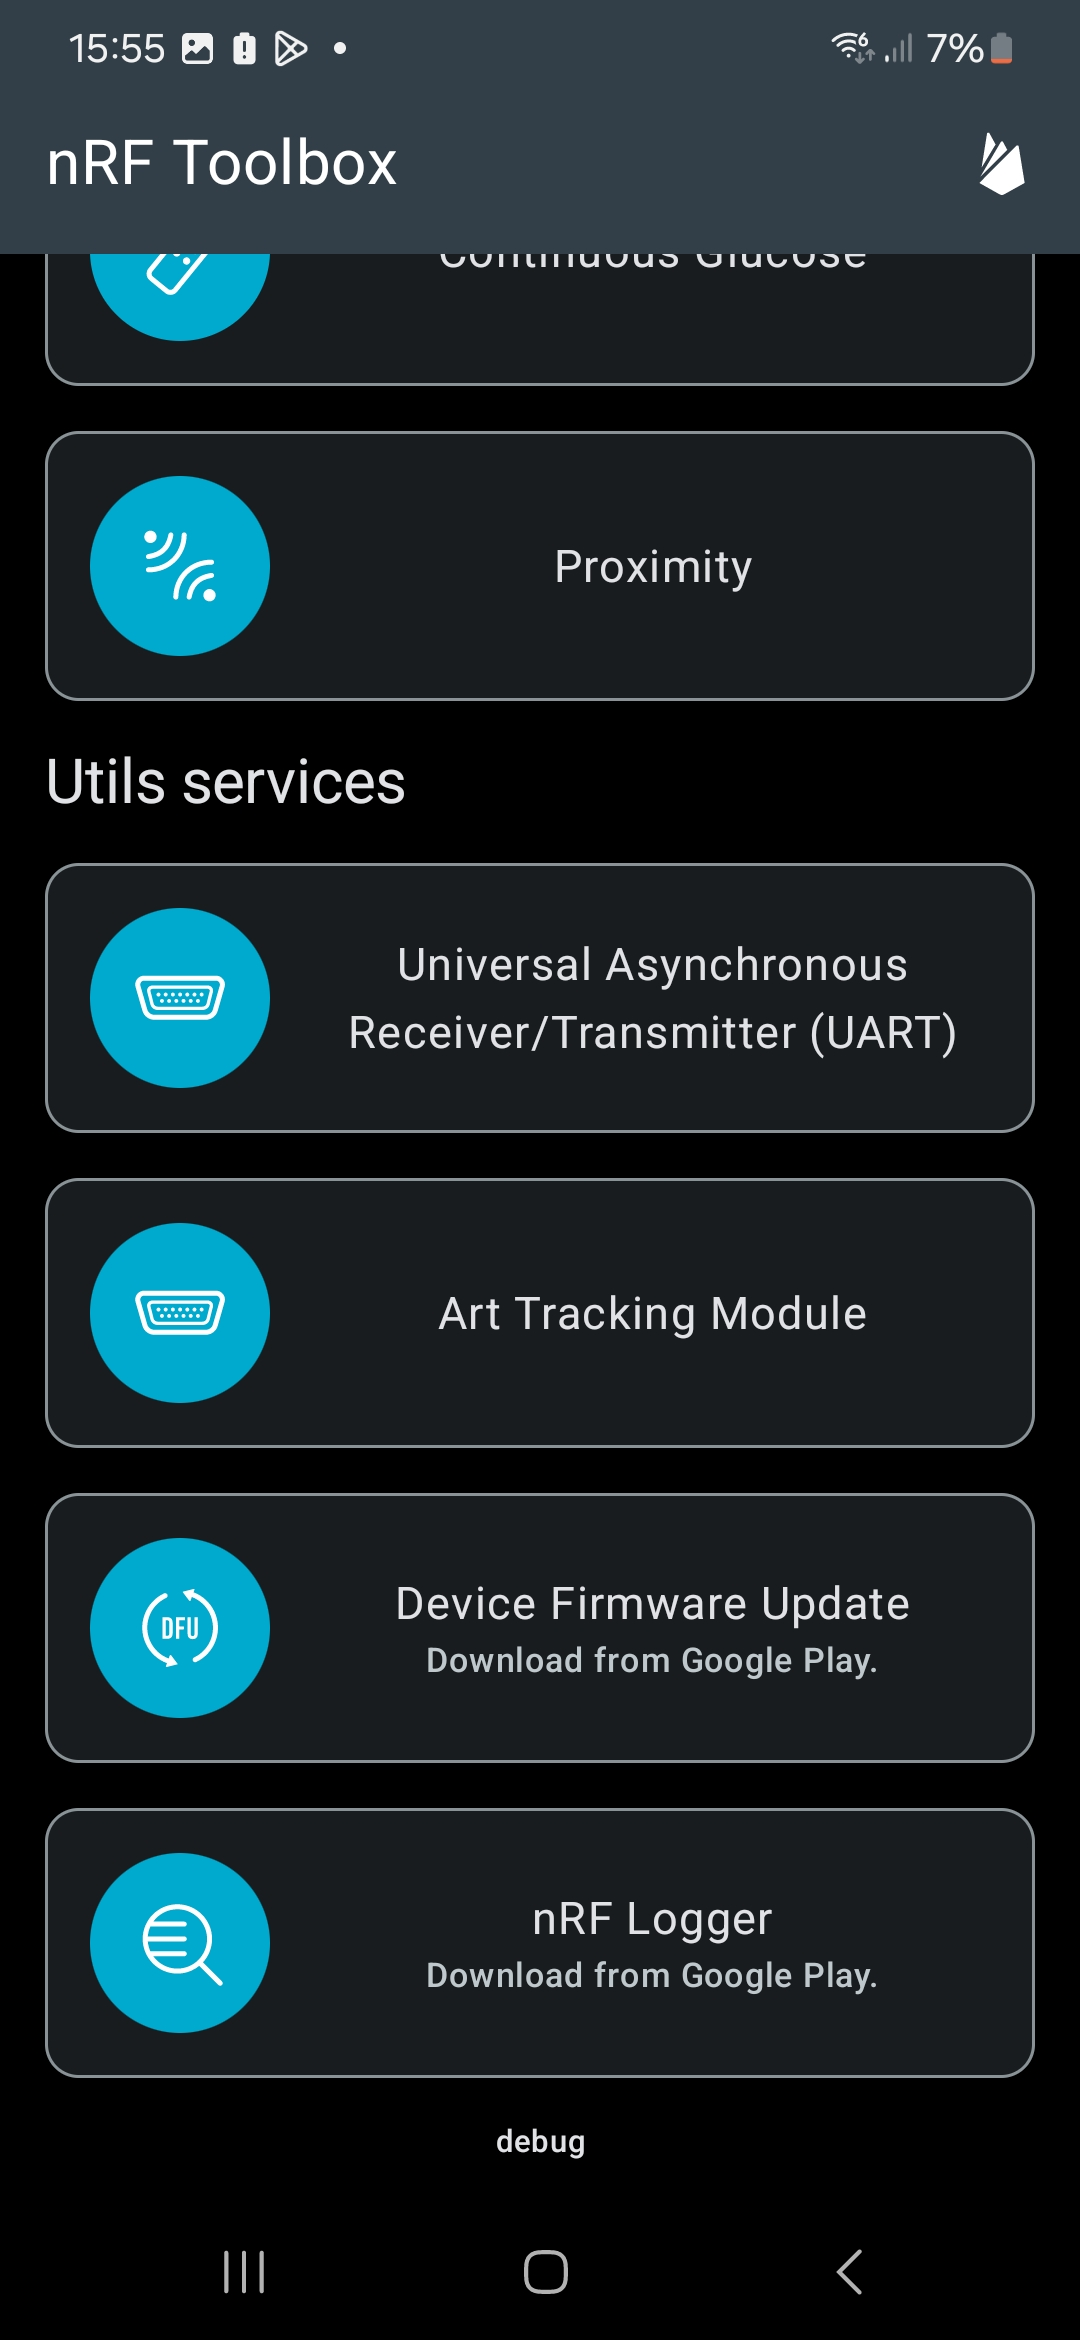
\includegraphics[trim={0 4cm 0 3cm},clip, width=.4\linewidth]{graphics/nRF_toolbox_modules.jpg}
	\caption{nRF Toolbox module menue, with the added Art Tracking Module}
	\label{f:Toolbox_modules}
\end{figure}

%The UART module is intended to be used with the ble\_ app\_ uart example.
Before discussing the new implementations, a description of the original UART module is provided to facilitate the understanding of the modifications in the art-tracking module.
When the UART module is opened, it shows all BLE services currently advertised and allows the user to connect to one of them \ref{f:Toolbox_connect}.
Once connected, it opens a window similar to phone messengers.
Here, it allows a keyboard input from the user and sends these messages to the connected devices (see \ref{f:Toolbox_output}).

%TODO A tiny bit of bullshit, why these are services are useful for the art-tracking app

\begin{figure}[ht!]
\centering
\begin{subfigure}{.4\linewidth}
	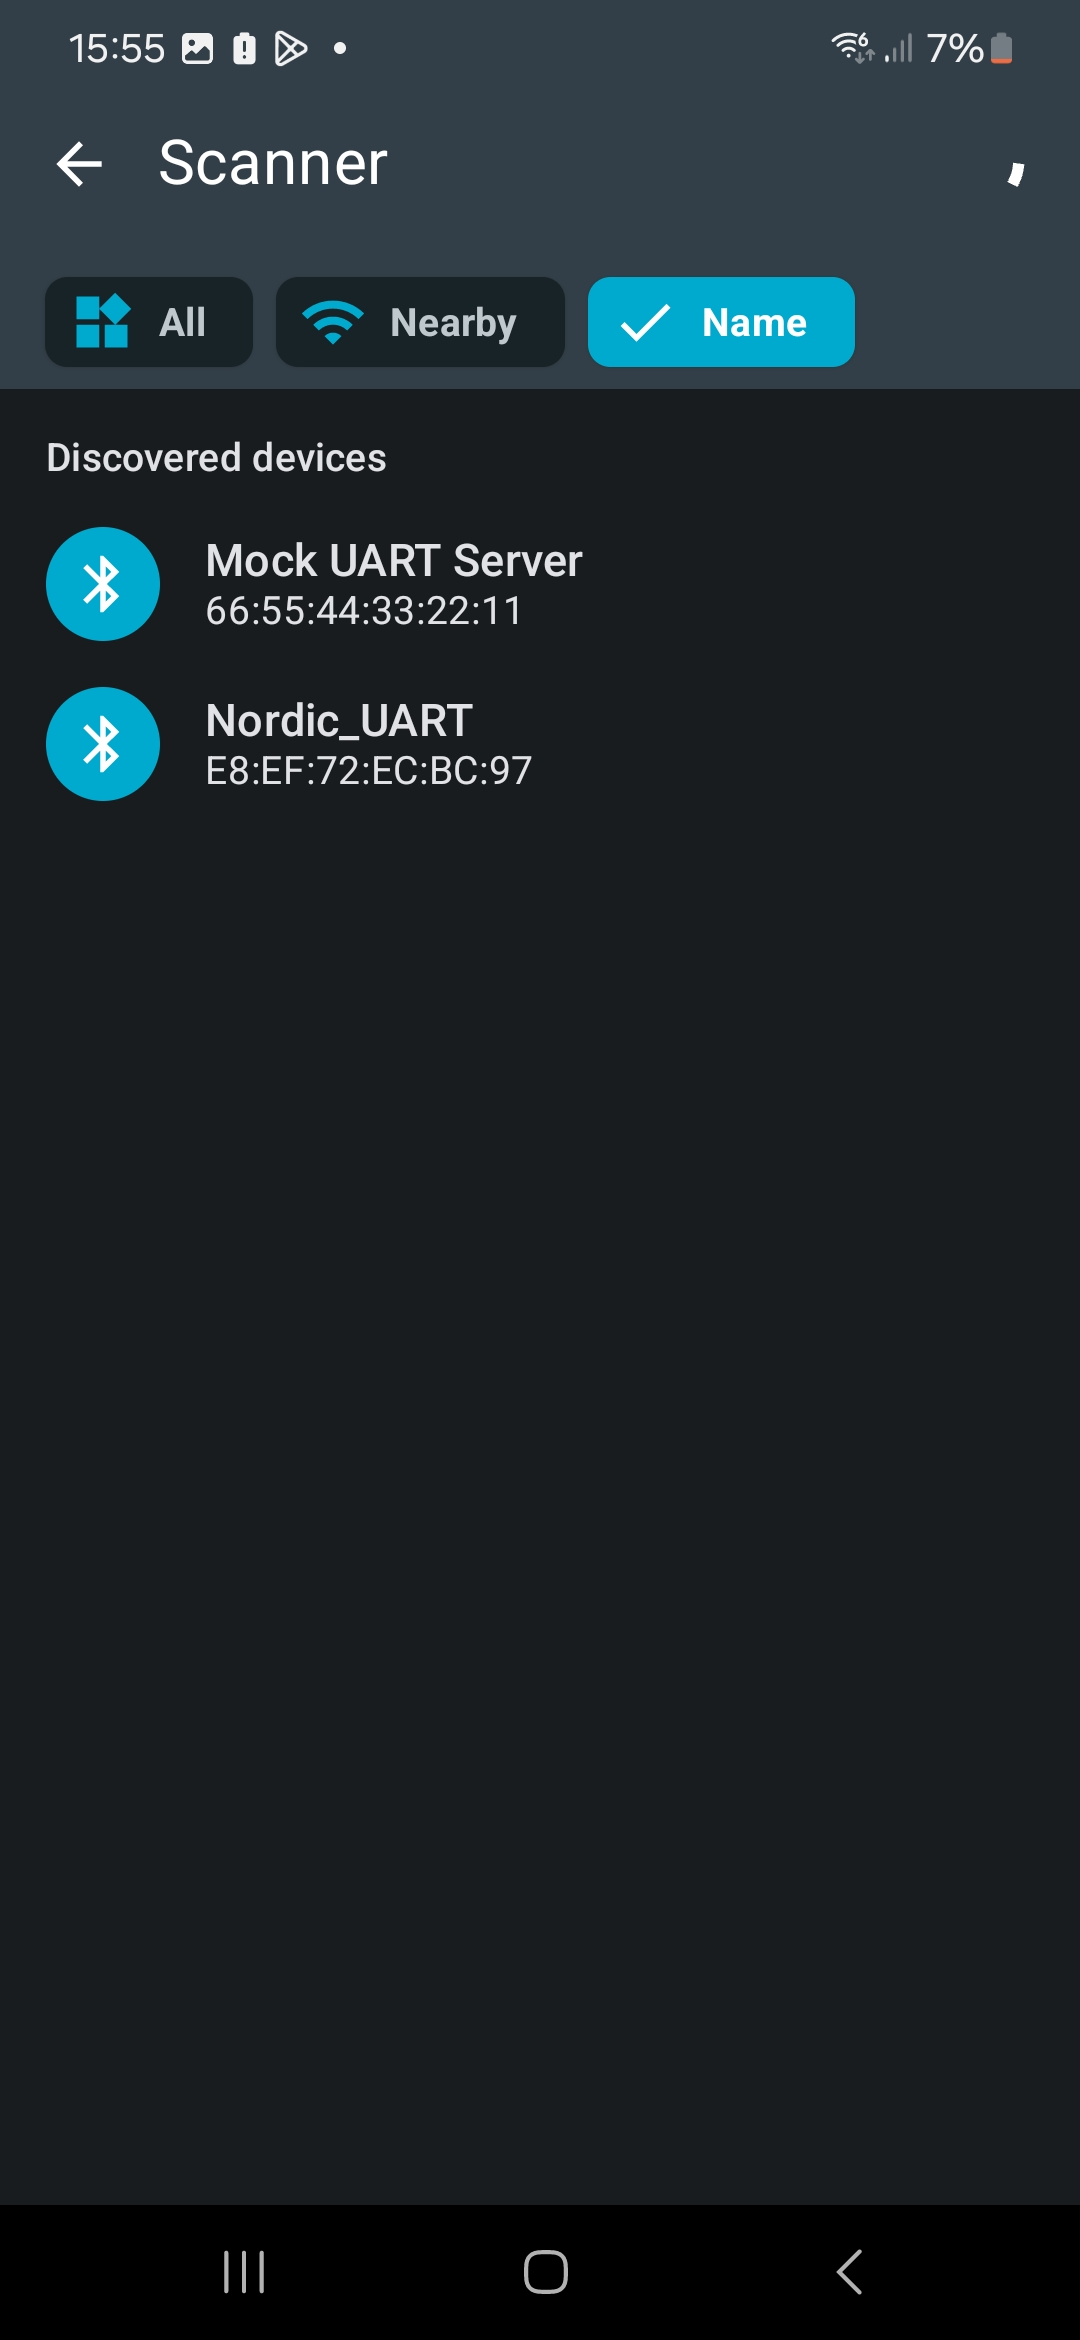
\includegraphics[trim={0 4cm 0 3cm},clip, width=\linewidth]{graphics/nRF_toolbox_connect.jpg}
	\caption{nRF Toolbox shows avaliable devices to connect to}
	\label{f:Toolbox_connect}
\end{subfigure}
\hspace*{.1\linewidth}
\begin{subfigure}{.4\linewidth}
	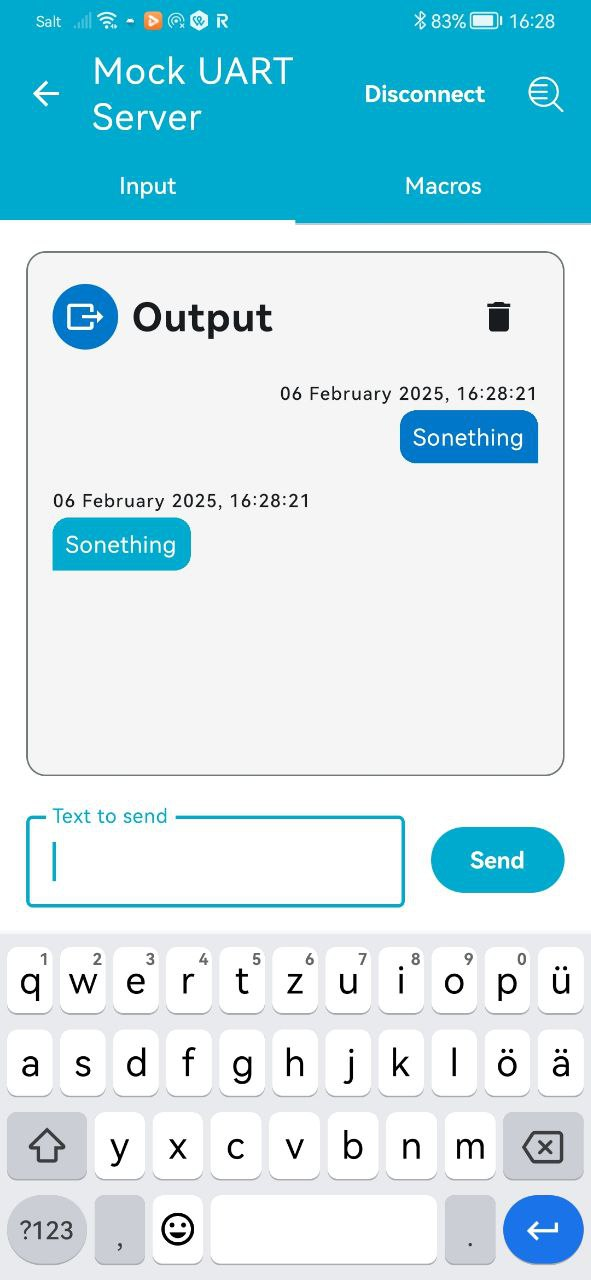
\includegraphics[trim={0 0 0 1.5cm},clip, width=\linewidth]{graphics/nRF_toolbox_messanger.jpg}
	\caption{nRF Toolbox UART module screen}
	\label{f:Toolbox_output}
\end{subfigure}
\end{figure}

The main differences of the art-tracking module to the UART module are after connecting to the relevant services.
So the are-tracking module opens up the same connection page as the UART module \ref{f:Toolbox_connect}, in which the user is able to select the BLE service and connect to it.

Once connected, instead of the UART module, the observation screen is shown (Figure \ref{f:Toolbox_art_tracking_empty}).
It also contains an output field, which will display messages.
At the bottom, seven parameters can be set: \textit{time}, \textit{max Temp}, \textit{min Temp}, \textit{max Hum}, \textit{min Hum}, \textit{max Angle}, \textit{max Dist}.
The parameters \textit{max}/\textit{min} \textit{Temp}/\textit{Hum} represent the expected range of humidity and temperature.
Any measurement outside these parameters will be considered a dangerous value by the app.
The tolerated difference in angle compared to the previous measurement is set by \textit{max Angle}, larger differences are considered dangerous values.
Distance measurement works analogously with \textit{max Dist} in meters.
The \textit{time} set defines the time that passes between measurements in seconds.
The default time is set to 350 seconds.
This means that the time passing between, for example, the temperature measurements on tag 2 is 350 seconds.


\begin{figure}[ht!]
\centering
\begin{subfigure}{.4\linewidth}
	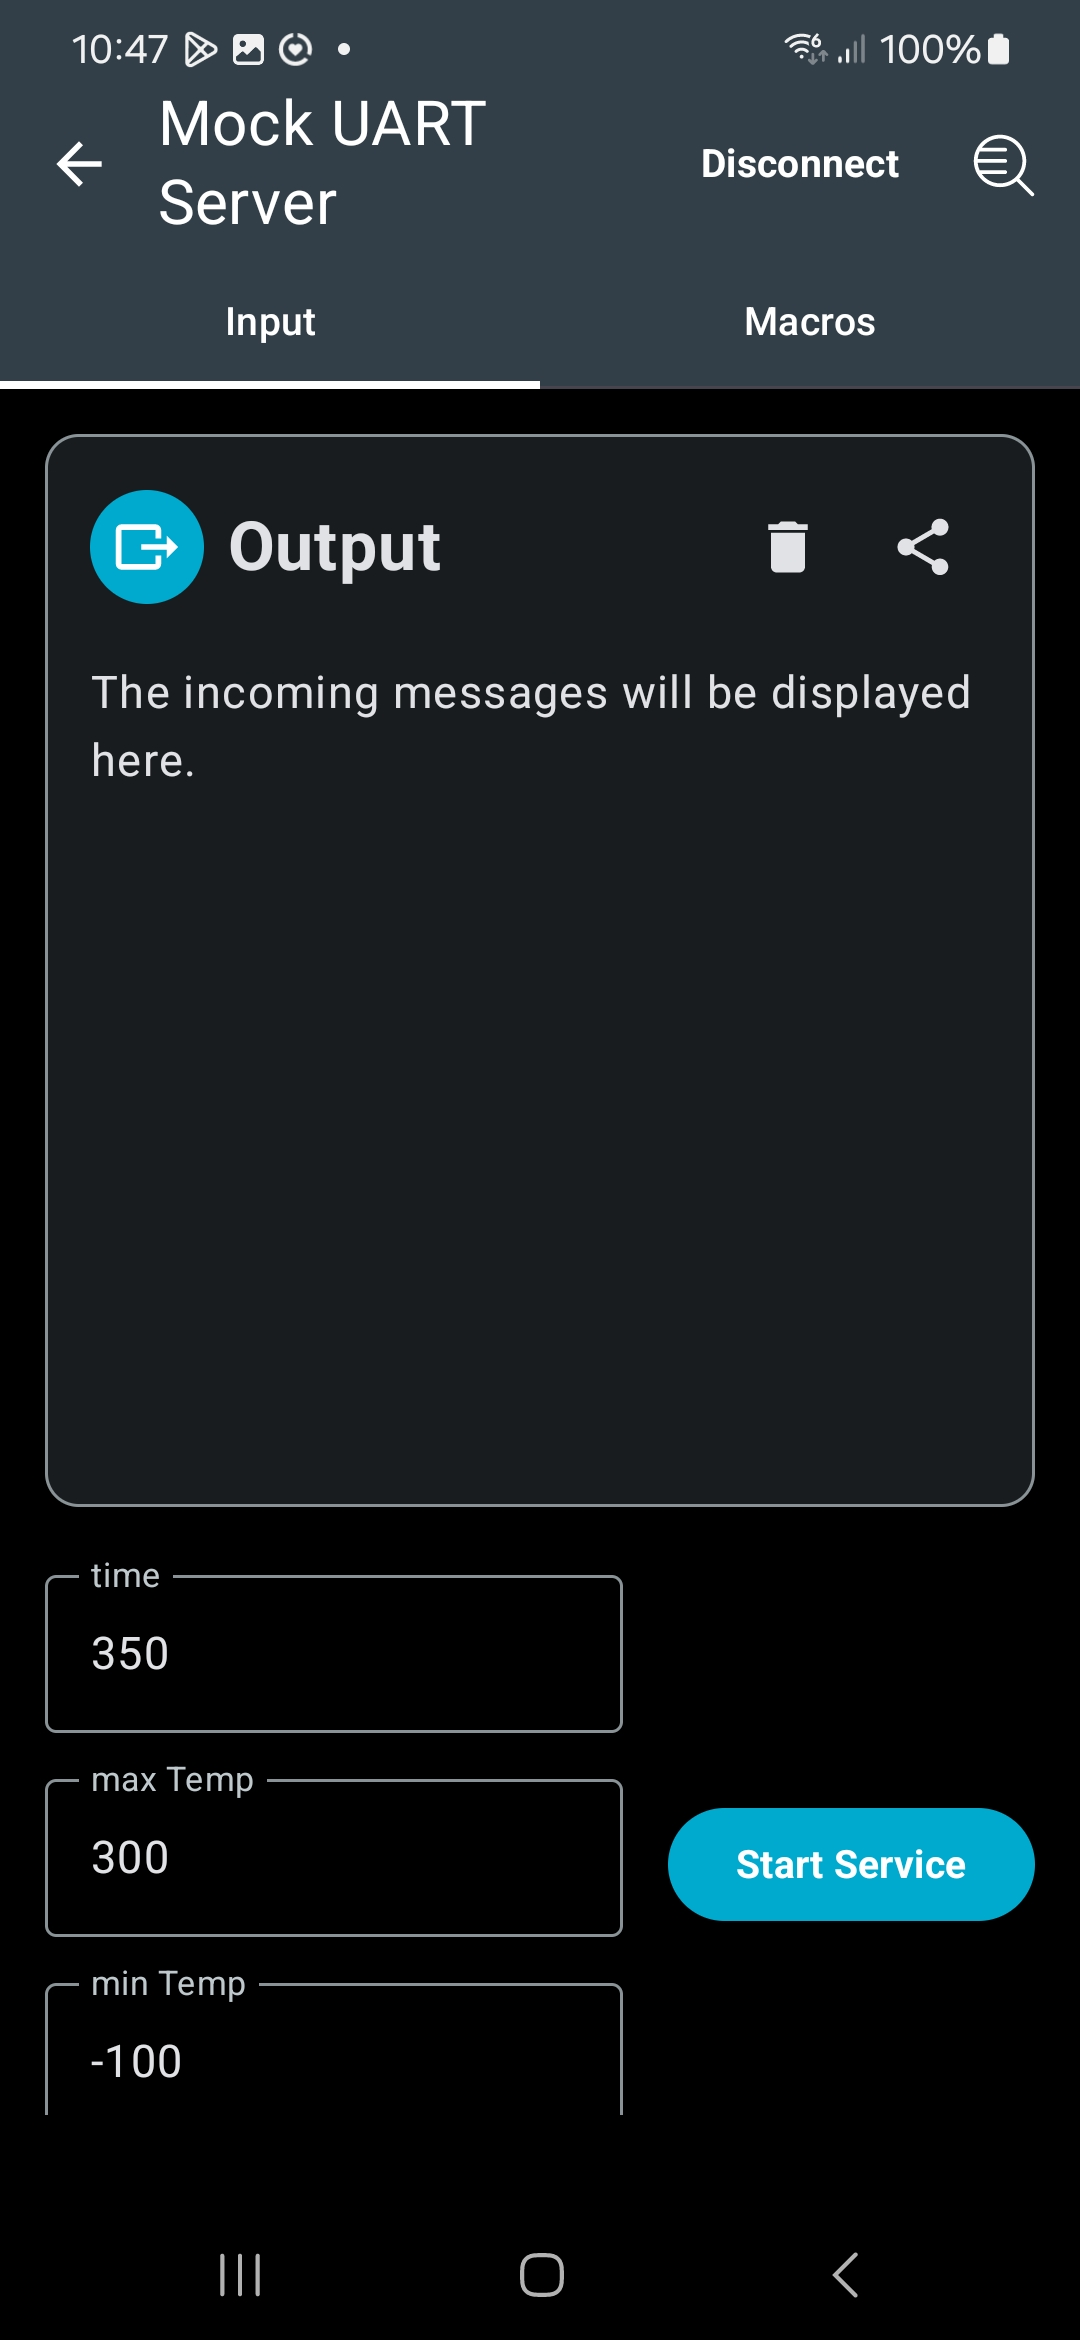
\includegraphics[trim={0 4cm 0 3cm},clip,width=\linewidth]{graphics/nRF_toolbox_art_tracking_empty.jpg}
	\caption{Art Tracking module oberservation screen before measurements}
	\label{f:Toolbox_art_tracking_empty}
\end{subfigure}
\hspace*{.1\linewidth}
\begin{subfigure}{.4\linewidth}
	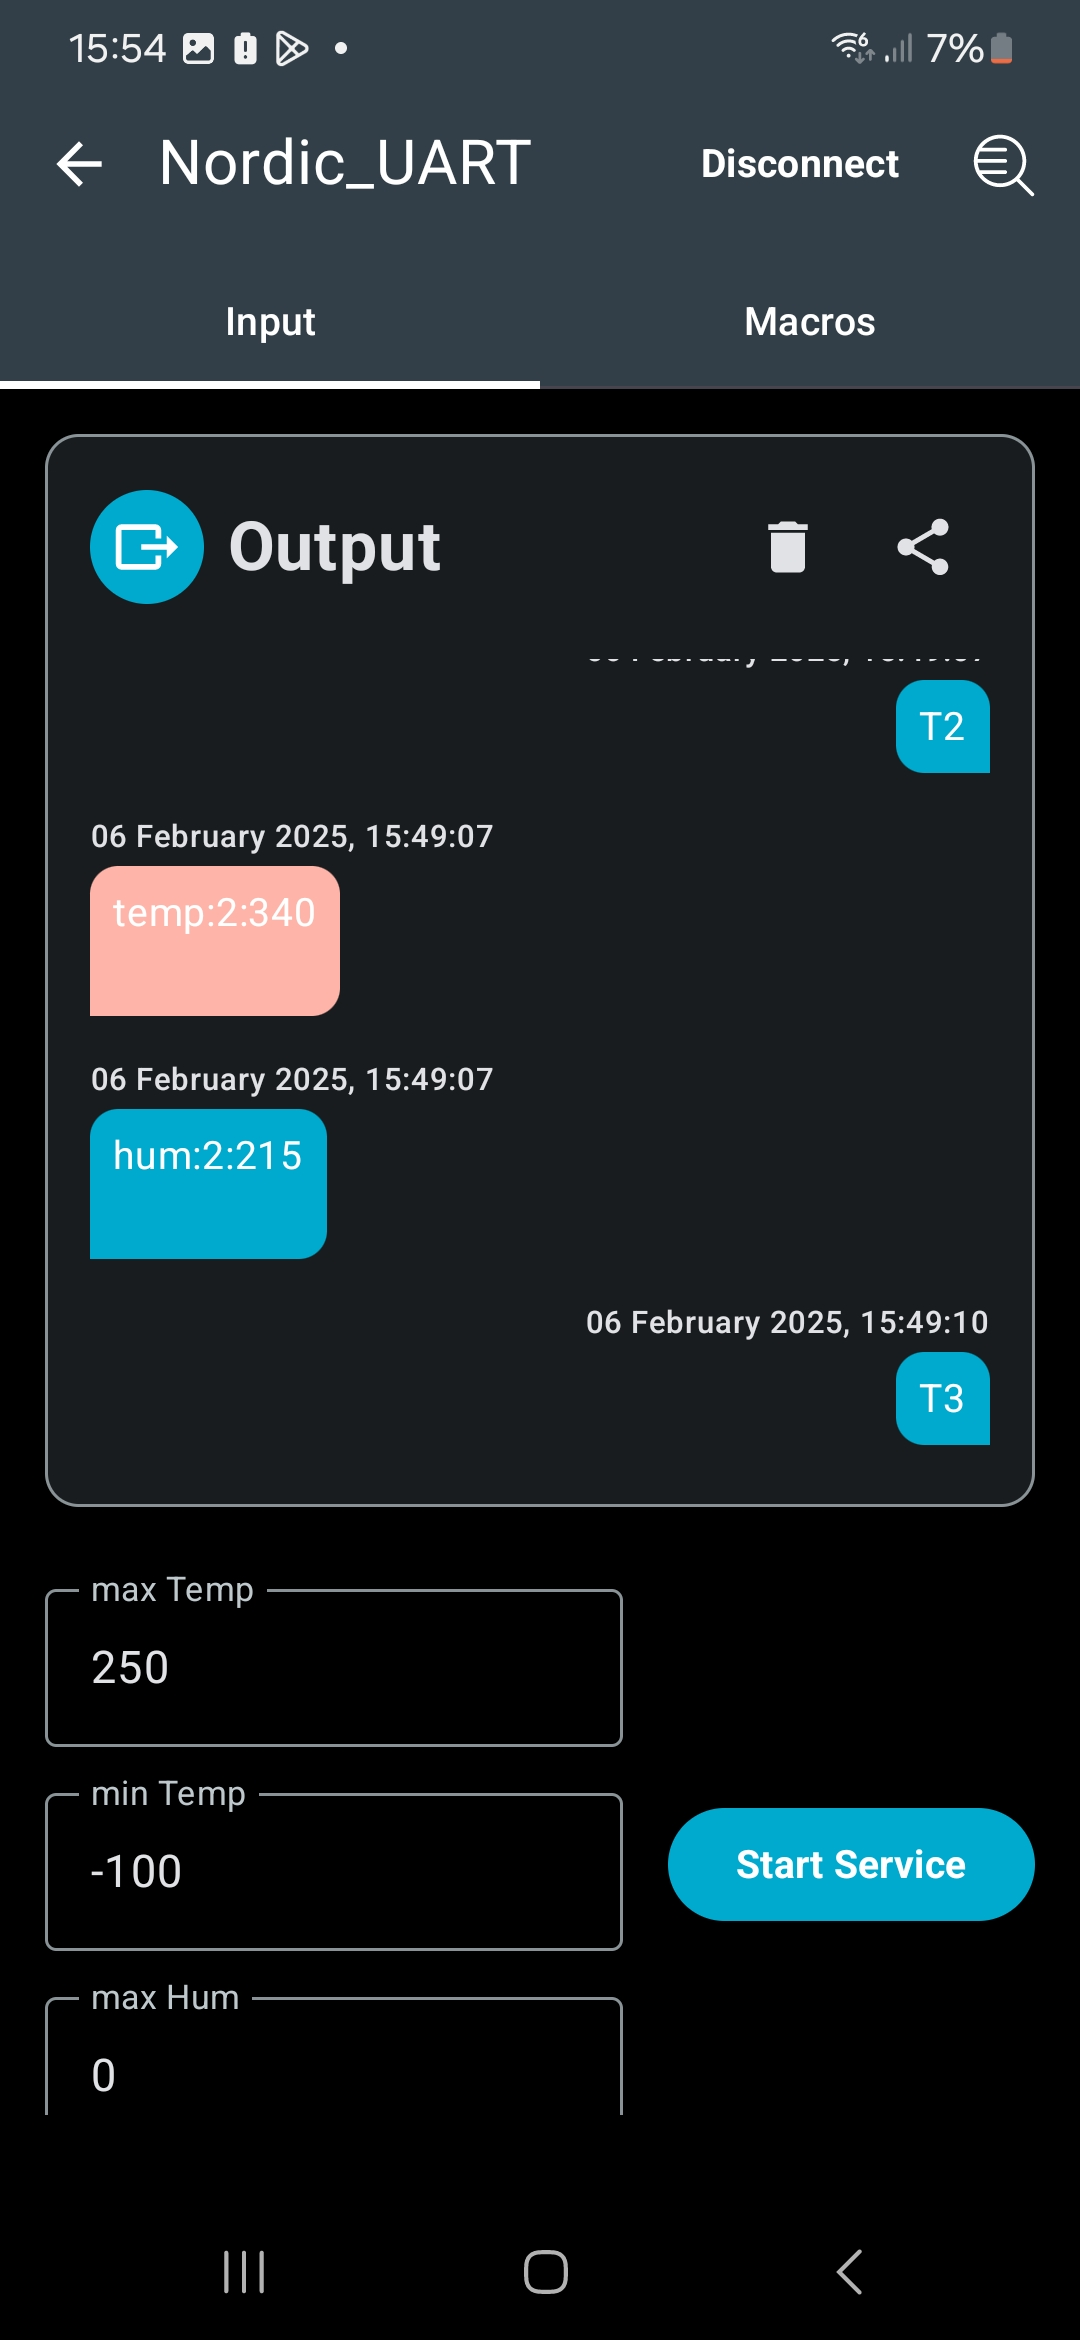
\includegraphics[trim={0 4cm 0 3cm},clip, width=\linewidth]{graphics/nRF_toolbox_Bad_Value_2.jpg}
	\caption{Art Tracking module, queries and responses}
	\label{f:Toolbox_art_filled}
\end{subfigure}
\end{figure}


When the user presses the \textit{Start Service} button, a program starts that periodically queries the tags for the measurements.
Once this process has started, the queries will appear in the chat window on the right side of the screen (see Figure \ref{f:Toolbox_art_filled}).
The current tag is mentioned on the right side and corresponding measurements are on the left side.
If the measurement is inside the set parameters, the message bubble will appear blue.
If the measured value is considered a dangerous value, the text bubble will appear red.
Since the message display is programmed in an asynchronous way, it can happen, that the answer to a query appears before the query itself, if the queried tag is the same as the tag connected to the phone.
This service can be stopped by pressing the \textit{start service} button again or by exiting this screen in any way.

The measurement loop for the output is shown in Figure \ref{code:App_main_loop}.
Each sensor is assigned a character.
\textit{T} for temperature and humidity, \textit{G} for gyro and \textit{D} for distance.
Each tag has a number, here from one to four since four tags were used in the experiments.
The loop concatenates these two characters and sends the resulting query to the connected tag.
Then the next tag-number is prepared for the next query.
Once all tags have been queried for a sensor, the tag-number starts with the first again and the next sensor is queried.
In between calls the app waits.
The call time for distance-measurement is fixed at 80 seconds.
Distance measurement takes longer than the other sensors, since for every devices three measurements need tobe conducted.
Additionally the sensors that do not participate in a ranging session are sleeping for a quite generous amount of time, to ensure they don't disturb the ranging session.
80 seconds has been chosen, since it allows enough time for all the ranging to happen, plus two repeats per sensor in case the ranging session fails.
For the other sensors, the waiting time in between queries is calculated from the remaining set time, after the ranging time is deducted.

\begin{figure}[h]
    \centering
    \begin{lstlisting}[language=Java]
    private val sensors = listOf("T", "G", "D")
    private val devices = listOf("1", "2", "3", "4")
    private var measurement_type = 0
    private var tag = 0
    private var timeBetweenCals: Long = 3750

    private val runnable = object : Runnable {
        override fun run() {
            if (tag >= list2.size) {
                tag = 0
                measurement_type += 1
            }
            if (measurement_type >= list1.size) {
                measurement_type = 0
            }
            val textToSend = "${list1[measurement_type]}${list2[tag]}"
            artRepository.sendText(textToSend, MacroEol.LF)
            tag += 1
            if(list1[measurement_type] == "D"){
                handler.postDelayed(this, 80000)
            } else {
                handler.postDelayed(this, timeBetweenCals)
            }
        }
    }
    \end{lstlisting}
    % Optionally, add a caption to the figure
    \caption{Section from the ArtMetricService.kt, main measurement loop}
	\label{code:App_main_loop}
\end{figure}


The query-answers are appended to a file that is safed in the app-storage.
The information appendded consits of: the queried tag, the returned values, a timestamp and if the value was unproblematic.
This functionality is intended for experimental evaluation. 
In a real word application, this data should be periodically backed up on a server in a compressed manner.
When pressing the share-button on the top right of the message-box \ref{f:Toolbox_art_filled}.
It will open the Android naitive share functionality, to share the file over mail, an installed messanger, save it to onedrive or send it over Bluetooth.
In this project all files were sent with email.
Pressing the trashcan next to it will delete the chat and empty the file.
This allows the user to distinguish between different testing session.

%TODO: add image that shows an example file
%\chapter{Evaluation}
\label{chap:evaluation}

Five experiments were performed to validate the functionality of the tags.
The first is non specific and ment to test the setup in a stable environment.
Experiments two to four are intended to test the detection of unwanted circumstances.
Experiment five is tests the system in a real-world environment.
The experiment results were stored on the phone and then exported using email.
The analysis of the data and creation of graphs was then performed using a Jupiter Notebook, using Pandas and Pyplot for datamanagment and the creation of graphs.\\
For all experiments the query-frequency was set to 330s.
The measurements queries are spread across this timeframe.
Each experiment lasted between 40 minutes and one hour.
All eperiments were performed two to three times.
In each section only the data-set from the first experiment run is presented fully.
The other experiments will be mentioned only, if they have differing data or to confrim an unexpected datapoint.

The tags used were programmed as described in Chapter \ref{c:implementation}.
The same four tags were used for all experiments.
They will be refered to as Tag-1, Tag-2, Tag-3 and Tag-4.





\section{Experiment 1: Static}
\label{ss:exp_1}
The four tags where placed on the corners of a 80 cm by 50 cm rectangle on a wooden table.
Figure \ref{f:exp1_schematic} shows a schematic view of the setup.
Each tag was turned on sequentially and given enough time to establish the network.
The phone then was connected to Tag-4.
The parameters in the app were left unchanged.
The default parameters are large enough, that no measurement should be able to trigger a warning.
Orientational reading was used for the output of the gyroscope.
The setup was then left untouched for 35 min.
The goal of this experiment was, to gauge by how much the measurements can vary in a static environment.

\begin{figure}[ht!]
	\centering
	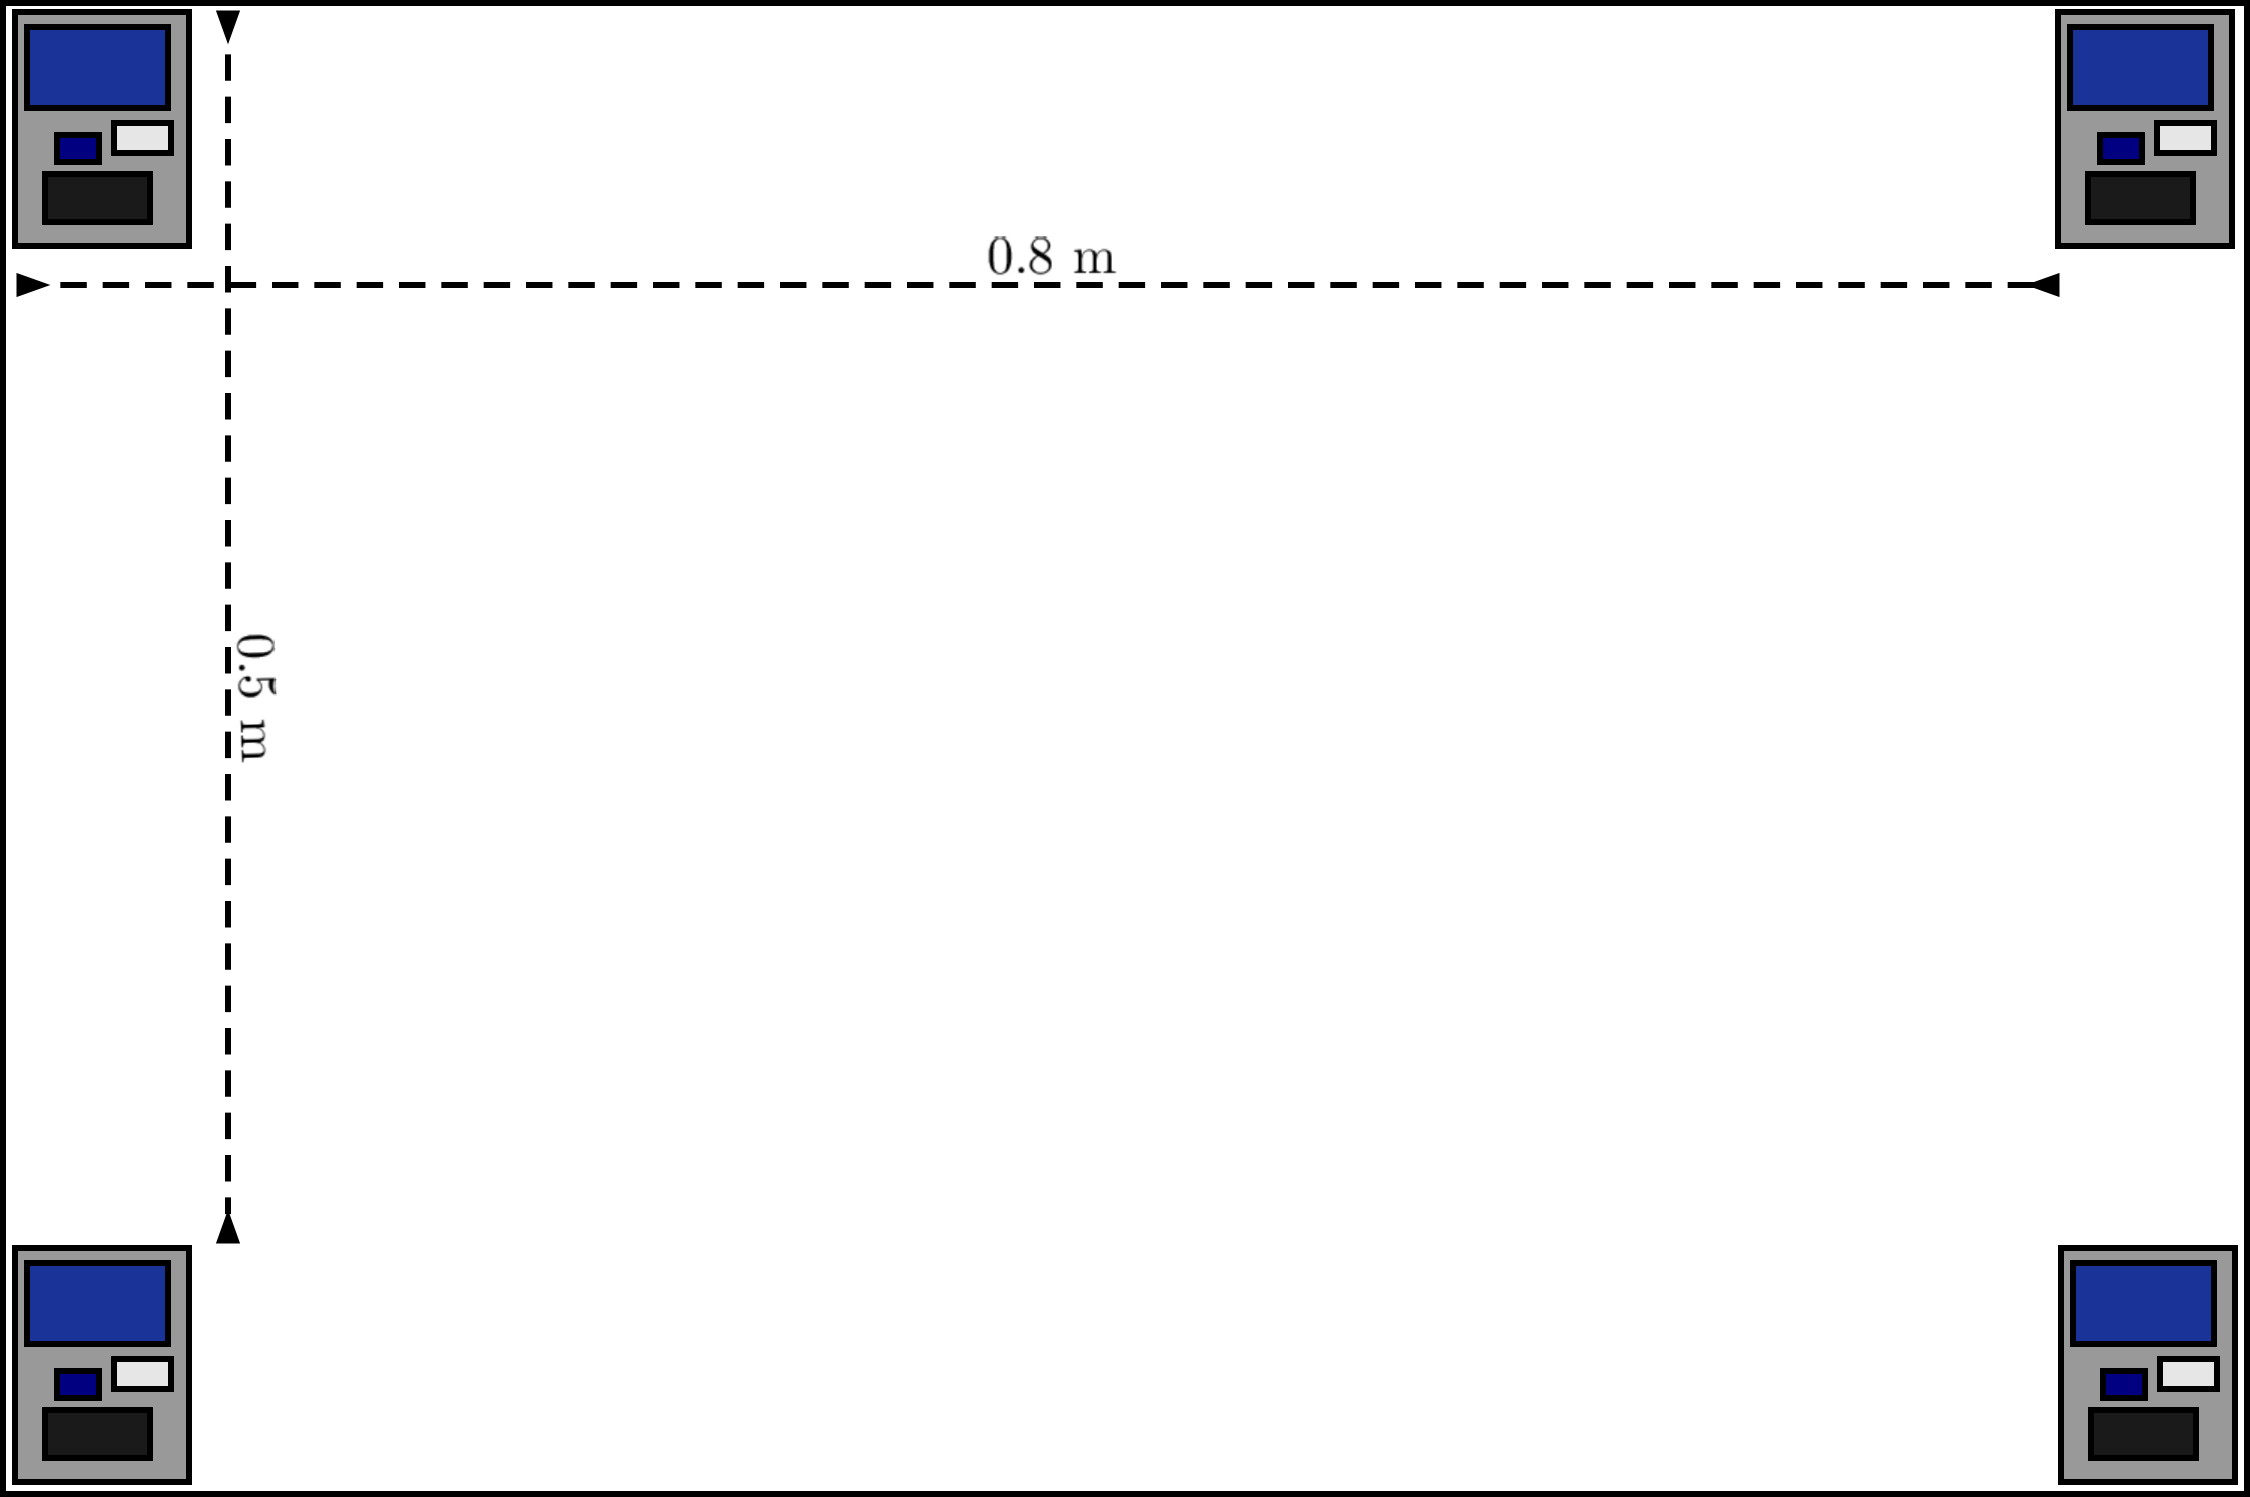
\includegraphics[width=300px]{graphics/schematics/experiment_1.png}
	\caption{Schema of the setup of experiment 1.}
	\label{f:exp1_schematic}
\end{figure}


\subsection{Results}
\label{ss:exp_1_result}
In eperiment one, all measurements are expected to be unchanging.
Table \ref{t:exp1_means} shows the mean values for temperature, humidity and angle during the experiment by tag.
Figures \ref{f:exp1_graphs_temp}, \ref{f:exp1_graphs_hum}, \ref{f:exp1_graphs_gyro}, \ref{f:exp1_graphs_dist} shows the change of these values over time.

\begin{table}[ht]
\centering
\caption{Mean and Variances for Temperature and Humidity Data by Tag during experiment 1.}
\begin{minipage}{0.45\textwidth}
\centering
	\begin{tabular}{|c|c|c|}
		\hline
		\textbf{Tag} & \textbf{Temp} & \textbf{Hum} \\
		\hline
		Tag-1 & 22.06 & 32.56 \\
		Tag-2 & 21.90 & 33.93 \\
		Tag-3 & 22.06 & 32.94 \\
		Tag-4 & 21.87 & 32.80 \\
		\hline
	\end{tabular}
	\caption*{Mean}
\end{minipage}
\hfill
\begin{minipage}{0.45\textwidth}
\centering
	\begin{tabular}{|c|c|c|}
		\hline
		\textbf{Tag} & \textbf{Temp} & \textbf{Hum} \\
		\hline
		Tag-1 & 0.02 & 0.03 \\
		Tag-2 & 0.05 & 0.04 \\
		Tag-3 & 0.03 & 0.06 \\
		Tag-4 & 0.03 & 0.05 \\
		\hline
\end{tabular}
\caption*{Variance}
\end{minipage}
\label{t:exp1_means}
\end{table}

\begin{figure}[ht!]
	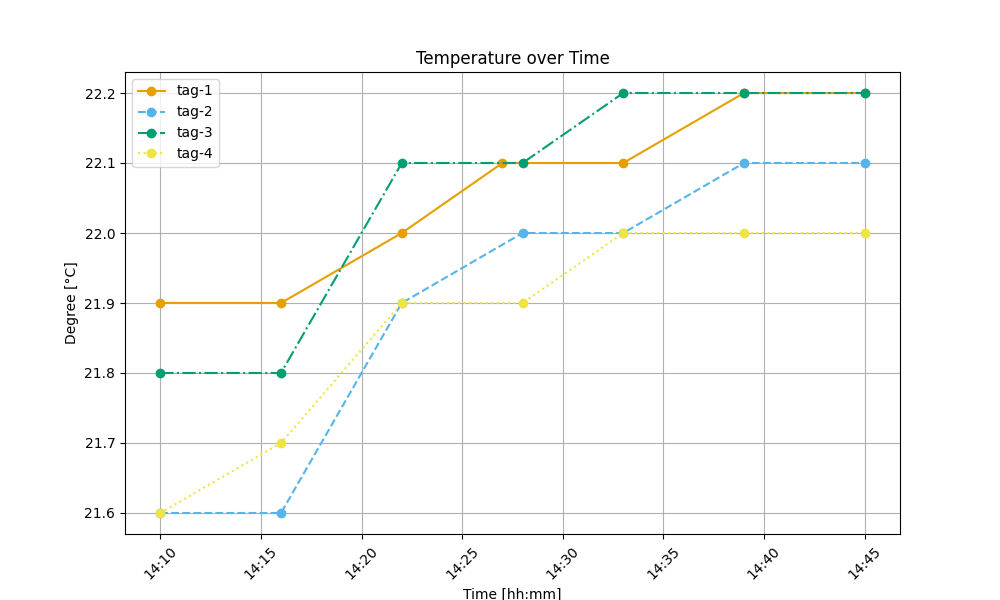
\includegraphics[width=\linewidth]{graphics/exp/exp1_temp_plot_0.png}
	\caption{Experiment 1, temperature over time.}
	\label{f:exp1_graphs_temp}
\end{figure}

Figure \ref{f:exp1_graphs_temp} shows the recorded temperature during experiment 1.
The tags are color coded and use different line-styles.
To make it easier to distinguische the lines, the Y axis only displayes the relevant section, rather then starting at 0\degree .
The time at the bottom represents the timestamp at which the measurement arrived at the phone.
All four tags have a mean temperature between 21.8 and 22.1 \degree C.
The varaince are also small, tag two having the highest one with 0.05 \degree C variance. 
The graph shows that all tags have a rising temperature.
The increase is quite small with tag two having the biggest increase of 0.5 \degree C over 20 minutes.
When the experiment was repeated,, the means stayed similar between the tags and the variance became only smaller.
The trend in temperature changed from upwards to downwards, when the experiment was repeated.

\begin{figure}[ht!]
	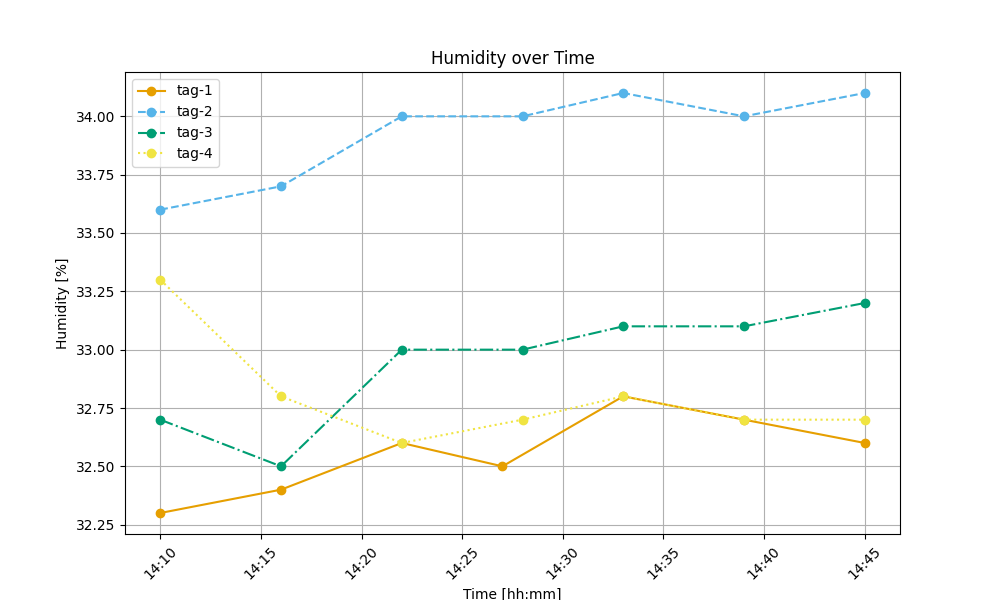
\includegraphics[width=\linewidth]{graphics/exp/exp1_hum_plot_0.png}
	\caption{Experiment 1, humidty over time.}
	\label{f:exp1_graphs_hum}
\end{figure}

Figure \ref{f:exp1_graphs_hum} shows the change of humidity over time.
Again, the relevant section of the y-axis is shown, rather than the full 0\% to 100\% , to increase readability.
The humidity of all sensor was similar as well.
The highest humidity was recorded by Tag-2 with 33.93\% .
Te lowest was recorded by Tag-1 with 32.56\% .
The variance is small, with Tag-3 having the biggest variance with 0.06\% pt.
During the first experiment, humidity increased by a small amount.
When the experiment was repeated,, the humidity dropped during the experiment.


\begin{figure}[ht!]
	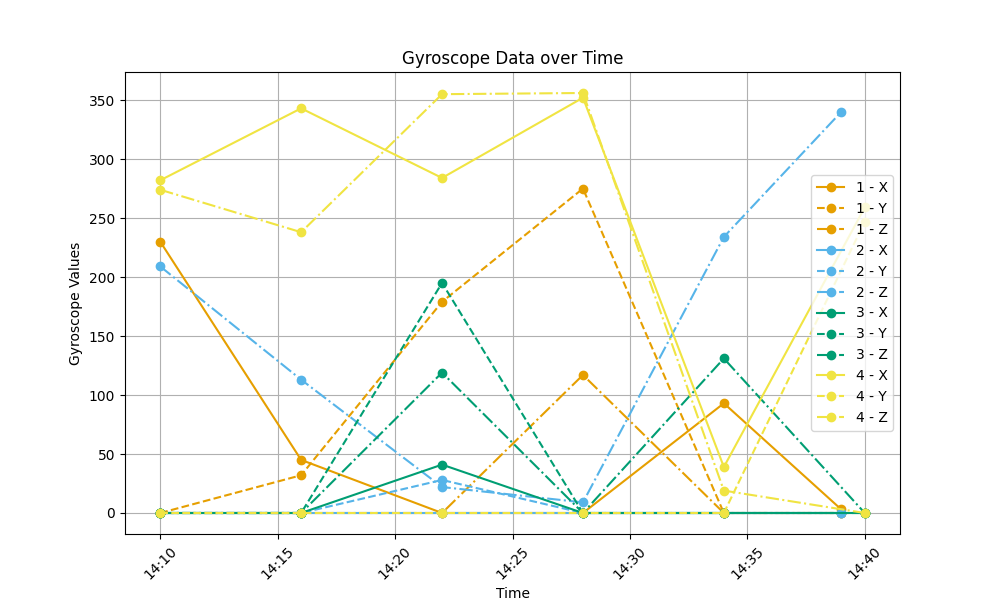
\includegraphics[width=\linewidth]{graphics/exp/exp1_gyro_data_plot_0.png}
	\caption{Registered value of the gyroscope over time during experiment 1.}
	\label{f:exp1_graphs_gyro}
\end{figure}

Since all tags were stationary during the experiment, the gyro sensor was expected to be unchanging.
This is not what occured.
The graph \ref{f:exp1_graphs_gyro} shows the values of the Gyroscope during experiment 1.
Orientational read was used, so the values shoud correspond to the angle around the given axis.
Each tag is assigned a color, and all angle measurements are shown in that color.
All X-axis measurement are diplayed using a filled line.
Axis-Y uses dotted lines.
Point-dotted lines represent the angles around axis-Z
Looking at the graph \ref{f:exp1_graphs_gyro} it is clear, that the measurement shows a wide range of angles for each tag and axis.
The angle of axis-X, Tag-1 (filled orange line) for example, jumps from a value of 230 \degree to 45 \degree, 0 \degree, then stays at 0 \degree for one measurement, goes up to 93 \degree and drops down again to 3 \degree.
As can be seen with this example is, that the measurements also don't fall a clear tragetory.
Tag-1 switches between rising and falling.
The only exception is tag 2 around the x axis, which stays at 0 for the whole measurement duration.\\
Since angle measurements fall into modular arithmetic, it "wrappes around" at 360\degree , means can only meanigfully be taken if the angles are in a small range.
Since this is not the case for most tags, the only mean that is meaningfull is tag 2 axis-x, which has a mean of 0 and a variance 0.

\begin{figure}[ht!]
	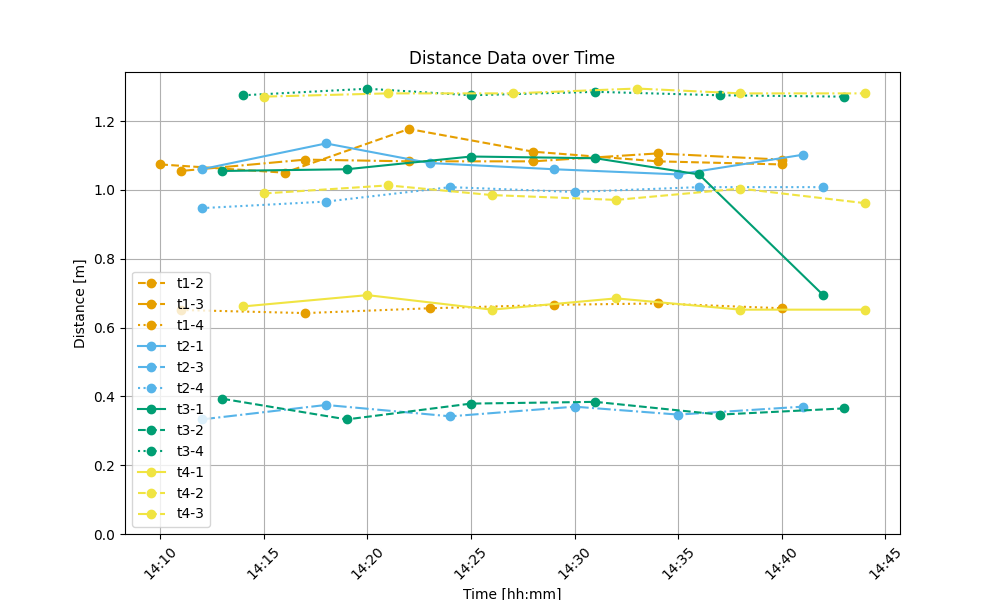
\includegraphics[width=\linewidth]{graphics/exp/exp1_dist_data_plot_0.png}
	\caption{Experiment 1, distance over time.}
	\label{f:exp1_graphs_dist}
\end{figure}

\begin{table}[ht]
\centering
	\caption{Mean, excpected values and variance of distant measurements, experiment 1.}
\begin{minipage}{0.45\textwidth}
	\begin{tabular}{|c|c c c c|}
		\hline
		& \textbf{Tag-1} & \textbf{Tag-2} & \textbf{Tag-3} & \textbf{Tag-4} \\
		\hline
		\textbf{Tag-1} & 0.0 & 1.094 & 1.084 & 0.657 \\
		\textbf{Tag-2} & 1.080 & 0.0 & 0.356 & 0.989 \\
		\textbf{Tag-3} & 1.007 & 0.367 & 0.0 & 1.279 \\
		\textbf{Tag-4} & 0.666 & 0.987 & 1.281 & 0.0 \\
		\hline
	\end{tabular}
	\caption*{Mean}
\end{minipage}
\hfill
\begin{minipage}{0.45\textwidth}
\centering
	\begin{tabular}{|c|c c c c|}
		\hline
		& \textbf{Tag-1} & \textbf{Tag-2} & \textbf{Tag-3} & \textbf{Tag-4} \\
		\hline
		\textbf{Tag-1} & 0.0 & 0.8 & 0.94 & 0.5 \\
		\textbf{Tag-2} & 0.8 & 0.0 & 0.5 & 0.94 \\
		\textbf{Tag-3} & 0.94 & 0.5 & 0.0 & 0.8 \\
		\textbf{Tag-4} & 0.5 & 0.94 & 0.8 & 0.0 \\
		\hline
	\end{tabular}
	\caption*{Excpected values}
\end{minipage}
\hfill
\begin{minipage}{0.45\textwidth}
	\centering
	\begin{tabular}{|c|c c c c|}
		\hline
		& \textbf{Tag-1} & \textbf{Tag-2} & \textbf{Tag-3} & \textbf{Tag-4} \\
		\hline
		\textbf{Tag-1} & 0.0 & 0.002 & 0.000 & 0.000 \\
		\textbf{Tag-2} & 0.001 & 0.0 & 0.000 & 0.001 \\
		\textbf{Tag-3} & 0.024 & 0.001 & 0.0 & 0.000 \\
		\textbf{Tag-4} & 0.000 & 0.000 & 0.000 & 0.0 \\
		\hline
	\end{tabular}
	\caption*{Variance}
\end{minipage}
\label{t:exp1_dist_var}
\end{table}

Table \ref{t:exp1_dist_var}, shows the mean, excpected value and variance of the measured distances.
The tag listed in the row is the queried tag that initiates the distance measurement, and the row corresponding to the responding tag.
By looking to the measurements diagonaly oposed to each other, one can see that the measured distaances is the the same, indipendent of who initiated the measurement, up to a range of two centimeters. 
The measurements from Tag-3 to Tag-1 is the highest, with 0.024m. All other variances are negibly small, beeing bellow 0.005m.
This shows that the measured distances are constant and stable, escept for the measurement from Tag-3 to Tag-1.
The distances measured do not correspond to the actual distances the tags had to each other, also seen in table \ref{t:exp1_dist_means}.
The measured distances can be as far of as 0.5 meters.
The two larger distances, 0.8 and 0.94 meters, correspond to the two larger measured values for each tag, while the smallest measured value always corresponds to the smallest distance, 0.5 meters.
The two larger values are not always ordered correctly, 0.94 meters sometimes beeing measured smaller then 0.8 meters.
In repeated experiments, all these facts stayed true.


Figure  \ref{f:exp1_graphs_dist} shows the measured distance over time.
A label i-j informe that tag-i initiated the measurement, and the distance between tag-i and tag-j was measured.
All measurements initiated by Tag-1 are orange. The meausrements of Tag-2 are blue, Tag-3 green and Tag-4 yellow.
The second tag that is involved in the measurement is signified by the line.
Measurements to Tag-1 use filled lines. Measurements to Tag-2 use dashed lines, Tag-3 uses dashed and dotted lines and Tag-4 uses dotted lines.\\
All lines except for 3-1 are horizontal  and show little variance.
Measurement 3-1 is also stable untl the last measurement, where a datapoint that is 0.35m lower than all previously recorded data is measured.
One can also see that not all measurements start at the same time.
The first measurement of distance 1-2 was registered at 14.10, while the first measurement of 4-3 was recorded at 14.15.
Each distance was measured seven times and with equidistance measurement times.

\begin{figure}[ht!]
	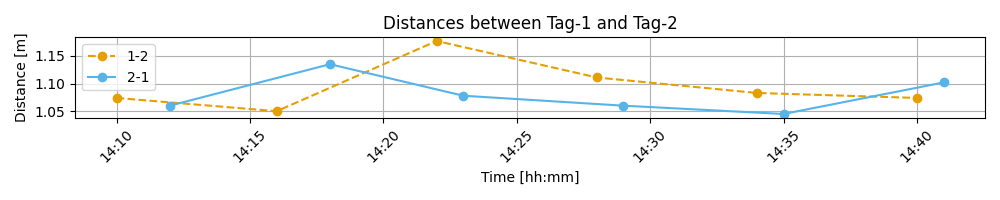
\includegraphics[width=\linewidth]{graphics/exp/exp1_dist_data_plot_1_1_2_split.png}
	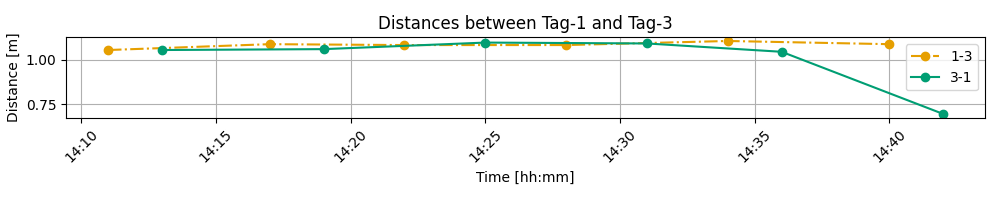
\includegraphics[width=\linewidth]{graphics/exp/exp1_dist_data_plot_1_1_3_split.png}
	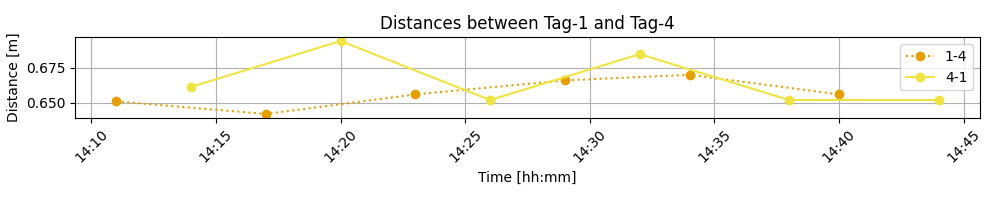
\includegraphics[width=\linewidth]{graphics/exp/exp1_dist_data_plot_1_1_4_split.png}
	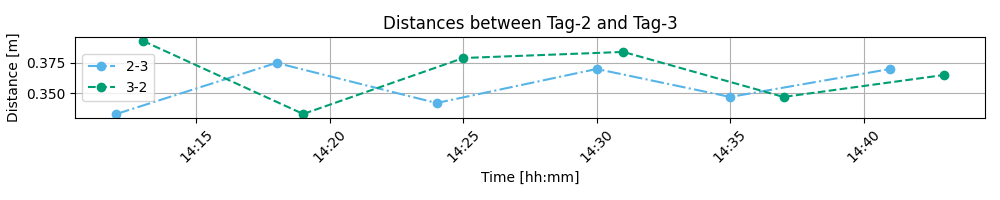
\includegraphics[width=\linewidth]{graphics/exp/exp1_dist_data_plot_1_2_3_split.png}
	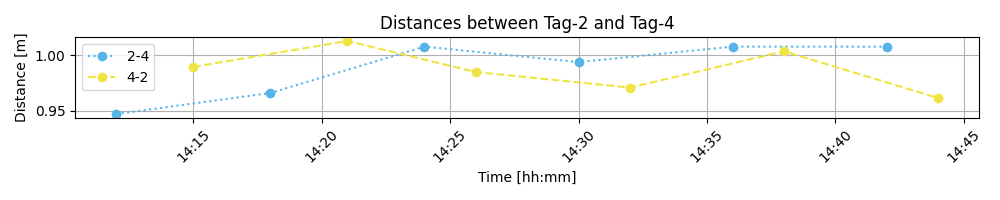
\includegraphics[width=\linewidth]{graphics/exp/exp1_dist_data_plot_1_2_4_split.png}
	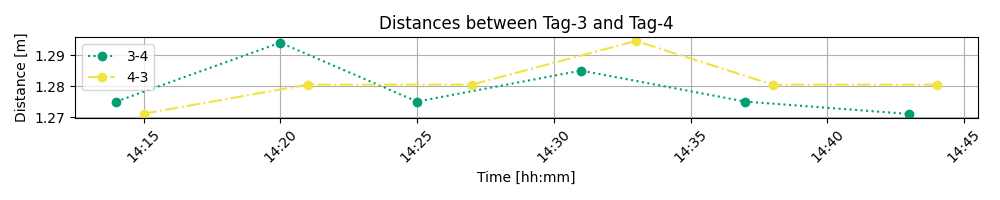
\includegraphics[width=\linewidth]{graphics/exp/exp1_dist_data_plot_1_3_4_split.png}
	\caption{Experiment 1, distance over time, for all pairs i-j.}
	\label{f:exp1_graphs_dist_split}
\end{figure}


The measurement pairs i-j and j-i report the same distance, but with different tags initiating the measurement. 
To better compare these pairs, figure \ref{f:exp1_graphs_dist_split} shows six subplots of figure \ref{f:exp1_graphs_dist} containing only each of these pairs.
The graphs show that the measurement pairs anre consistently close together.
One outlier happens when Tag-3 measures the distance to Tag-1 at very end of the measurements.
The measured value drops 0.35m bellow the previous mean of 1.30m.
When repeating this experiment and during other experiments, these outliers happened again, a bit less frequently then twice per hour.
The outliers always affected a measurement involving tag 1.

\begin{figure}[ht!]
	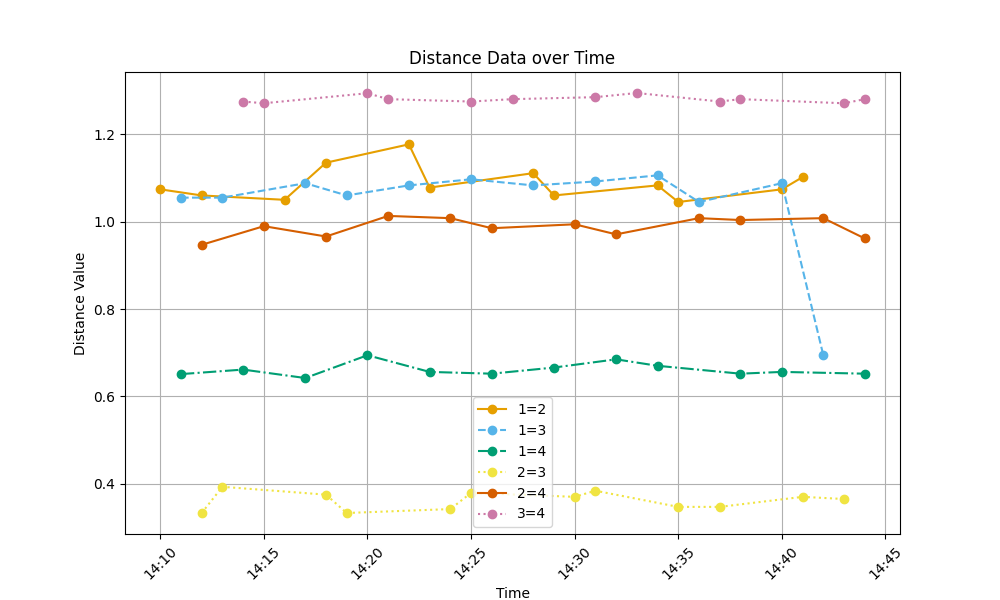
\includegraphics[width=\linewidth]{graphics/exp/exp1_dist_data_plot_1_combined.png}
	\caption{Experiment 1, distance over time, for comined pairs i=j.}
	\label{f:exp1_graphs_dist_combined}
\end{figure}

Since the pairs i-j and j-i report the same data and this fact is consistent in the measurements, they can be combined into one graph.
Figure \ref{f:exp1_graphs_dist_combined} shows the distances over time for all combined pairs i-j and j-i, called i==j.
Graphs like this will be called combined graphs in this report.
Since initiating and reseiving tag can no longer be distinguished, the line colors and types have no assigned meaning.
The two pairs 2=3 and 1=4 corresponding to the two low distances of 0.5m can be seen at the bottom.
The pairs 1=3 and 2=4 that represent the highest distance of 0.94m do not separate and are mixed together with 1=2 and 3=4.\\
Table \ref{tab:exp1_var_distanc} shows the means and variances of the combined tag pairs.
Since the measurements of i=j are the same as j=i, only the upper triangle of the distance-matrix is needed.
The table shows, that the variances are very low for all pairs, except 1=3.

\begin{table}[ht]
\centering
\caption{Statistics of the combined distance measurements between tags for experiment 1}
\begin{minipage}{0.45\textwidth}
\centering
\begin{tabular}{|c|c c c|}
\hline
		& \textbf{Tag-2} & \textbf{Tag-3} & \textbf{Tag-4} \\
\hline
\textbf{Tag-1}    & 0.112 & 0.265 & 0.177 \\
\textbf{Tag-2}   &  & 0.368 & 0.824 \\
\textbf{Tag-3}   &  &  & 0.385 \\
\hline
\end{tabular}
\caption*{Mean}
\end{minipage}
\hfill
\begin{minipage}{0.45\textwidth}
\centering
\begin{tabular}{|c|c c c|}
\hline
		& \textbf{Tag-2} & \textbf{Tag-3} & \textbf{Tag-4} \\
\hline
\textbf{Tag-1}    & 0.001 & 0.013 & 0.000 \\
\textbf{Tag-2}   &  & 0.000 & 0.000 \\
\textbf{Tag-3}   &  &  & 0.000 \\
\hline
\end{tabular}
\caption*{Variance}
\end{minipage}
\label{tab:exp1_var_distanc}
\end{table}


\subsection{Conclusion}
\label{s:exp1_conclustion}
The temperature measurement seem to be working as excpected.
All four tags show the same temperature, within a small margin of error.
Variance is low, showing a consistent temperature measurement.\\
Two possible explenations were found for the increase in temperature during the experiment.
One possible explenation is given by the fact, that this was the first experiment performed in the day, and the room temperature was slightly increasing because of the presence of a person, that was not present before.
An alternative explenation is, that the microprocessors proucde heat that was detected.
The fact that the temperature decreased during subsequent experiments, favors explenation one, since their would be no reason for the microcontrolers to stop producing heat.
The decrease itself can be explained, since during setup, the person performing the experiment was close to the sensor, while during the experiment the person stayed in a different part of the room. The dicrease in temperature was smaller, this difference in closness to body heat could explain the difference.


The humidity sensor similarly produced satisfactory results.
All four tags presented the same humidity, only with small margins of error.
The variance is again satisfactory, since it is very small, beeing bellow 0.05%.
The slight increase in humidity can again be explained by this beeing the first experiment of the day, and the person performing the experiment having wet hair from the rain.
This again weakenes the microcontoler heat theory, since rising temperature without adding moisture would only decrease the humidity.\\
The dicrease in humidity in subsequent experiments lacks a clear explenation.
It is a very weak trend, so factors global factors could explain the difference.
Changing weather conditions could account for the difference.
Another proposed explenation arises from the setup of the system.
During setup, each tag was touched repeatedly to put them into position.
The person performing the experiment tends to have clamy hands, that feasably could lead the sensors to detect additional humidity at the beginning of the experiment.\\
Without additional data, no one explenation can be favored over the other. 
Since the decrease in temperature was small, this is not considered a issue for this system.


The Gyroscoping sensor data does not produce any meaningfull result.
The measured orientation of the tags varied widely, while the physical tags stood still.
A possible explenation of this is, that the gyroscope used in the implementation has consistent biases.
Since the angular velocity is evaluated often and then added to the current angle, small errors would acumulate over time.
The time between measurements was 5 minutes and 30 seconds.
A bias of only $\frac{12}{11} \frac{\degreem}{s}$ would correspond to an accumulated error of 360\degree over this timespan.
Since rotational position in inheritly circular, rapping arround at 360 \degree, unless there was no variance next to the bias, the values would end sudo randomly scattered over the range of $[0\degreem , 360\degreem ]$.
The MPU6050 outpus only integers, so any bias at all would have this effect.\\
Be bias hypothoses is additionaly strengthend, by the existance of Tag-2 axis X, that stays at 0 over the course of the measurement.
While this could indicate a faulty sensor, during later experiments using rotational velocity readings, see section\ref{s:exp_5_real_world}, Tag-2 axis X did produce meaningfull results. While this doesn't disproove, that Tag-2 axis X was faulty during this experiment, it makes it more reasonable to assume, that it has a bias of 0. \\
A possible reason for the bias in angular velocity was considered, in the rotation of the earth.
After some consideration, this thesis was dropped, since the angular velocity introduced by the earth would acount for no more than $\frac{1}{240} \frac{\degreem}{s}$ around the X or Y axis, if standing on the equator, where the effect is strongest.\\
The bias explenation seems to be a reasonable and explaines the measured results.
As a consequence, the orientational read has to be considered usless.


The distance measurements have mixed results.
The fact that the tag pairs produce the same same reults is good.
Double sided two-way ranging is used, so during each ranging session both tags conduct single-sided two-way ranging and the results are combined.
It is therefore expected, that the device that initiates the ranging does not matter.\\
The fact that ranging sessions involving Tag-1 occasionaly produce inconsistent results can not directly be explained.
Different locations were used for the experiments and the tags did not always have the same position.
This means that an explanation envolving multi-path effect based on position can be rejected.
The possible explenation envolves a fault on the nRF52840 microcontroler or the DMW3000 shield. 
Since the final calculation relies on the timestamps recorded during the ranging, a possible explenation would be, that the clock of the nRF52840 sometimes faults, or that there is an issue with the clock line of the SPI connection.\\
The fact that the resulting distances are wrong is troublesome.
The proposed design that would calculate the position by solving a quadratic program relies on somewhat accurate distance measurements.
The likely reason for the distance measurements producing wrong results is the simplified calibration, that was used for the $d_{rx}$, $d_{tx}$ values, see Section \ref{ss:two_way_ranging}.
The fact that the distances still sort themself into high and low values correctly indicates, that some calibration has worked, but it is not granular enough to work for small distances.\\
The distance measurements can currently not be used to build a model of the tag positions.
If they can be used to detect movement can not be determined by the static experiment and requires the introduction of movement, see Experiment 4 \ref{s:exp4}


\section{Experiment 2: Temperature}
\label{ss:exp_2}

\begin{figure}[ht!]
	\centering
	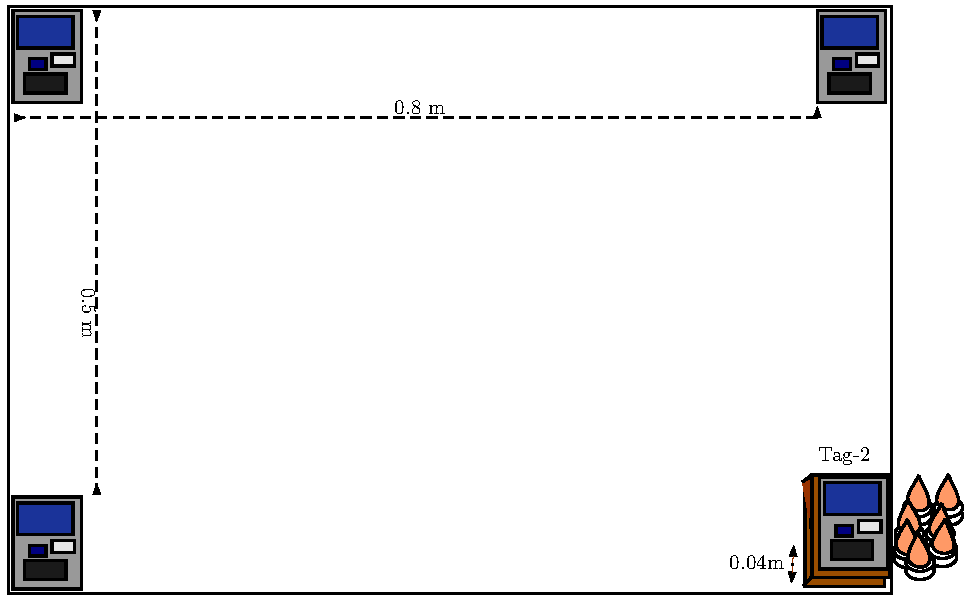
\includegraphics[width=300px]{graphics/schematics/experiment_2.pdf}
	\caption{Schema of the setup of experiment 2.}
	\label{f:exp2_schematic}
\end{figure}


The four tags were placed in the same 80 cm by 50 cm rectangle as in experiment one.
One tag placed on a elevated surface, 4 cm above the table.
next to the tag on the table, seven candles were placed (see figure \ref{f:exp2_photo} ).
Next to the Tag-2 thermometers detectors were placed.
Figure \ref{f:exp2_schematic} shows a schematic view of the setup.
Each tag was turned on sequentially and given enough time to establish the network.
The phone then was connected to one tag.
The max Temperature parameter in the app was changed to 35\degree C.
After 20 minutes the candles were lit.
The experiment was then left alone for another 30 minutes.
The independent thermometers were filmed during the process, to allow for later review and comparesment.
The goal of experiment 2 was to test the temperature detection capabilities of the system.

\begin{figure}[ht!]
	\centering
	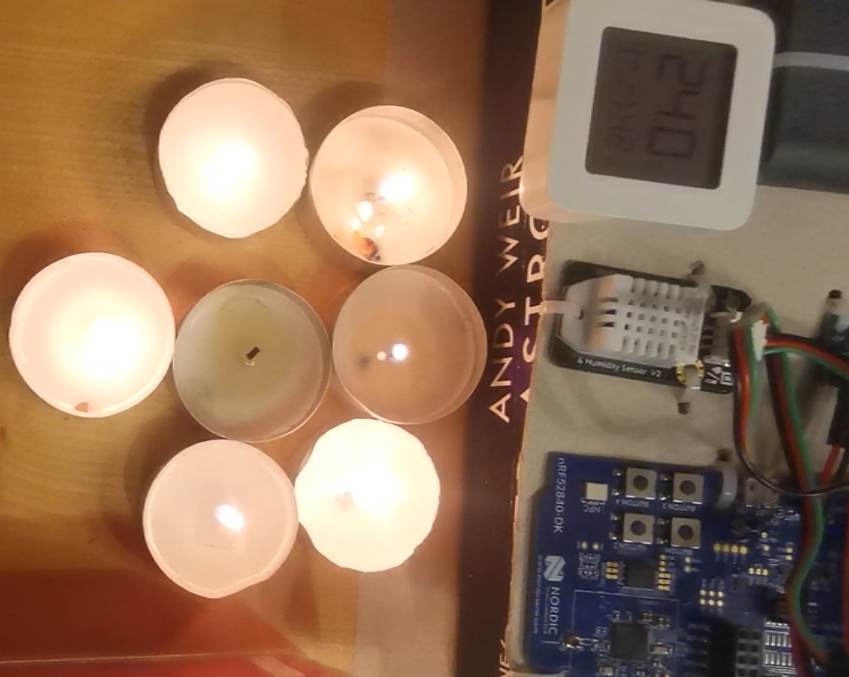
\includegraphics[width=300px]{graphics/exp/Exp_2_photo.png}
	\caption{Photo of elevated Tag-2, candles and thermoeter used in experiment 2.}
	\label{f:exp2_photo}
\end{figure}


\subsection{Results}
\label{ss:exp_2_result}
Experiment two introduced heat-sources to the system.
Since the main setup was the same as experiment 1 \ref{ss:exp_1_result}, many of the findings are the same.
In this section, only differences in results are discussed.
If a metric is not measioned, one can assume it behaved the same as for experiment 1  (see section \ref{ss:exp_1_result}).

\begin{figure}[ht!]
	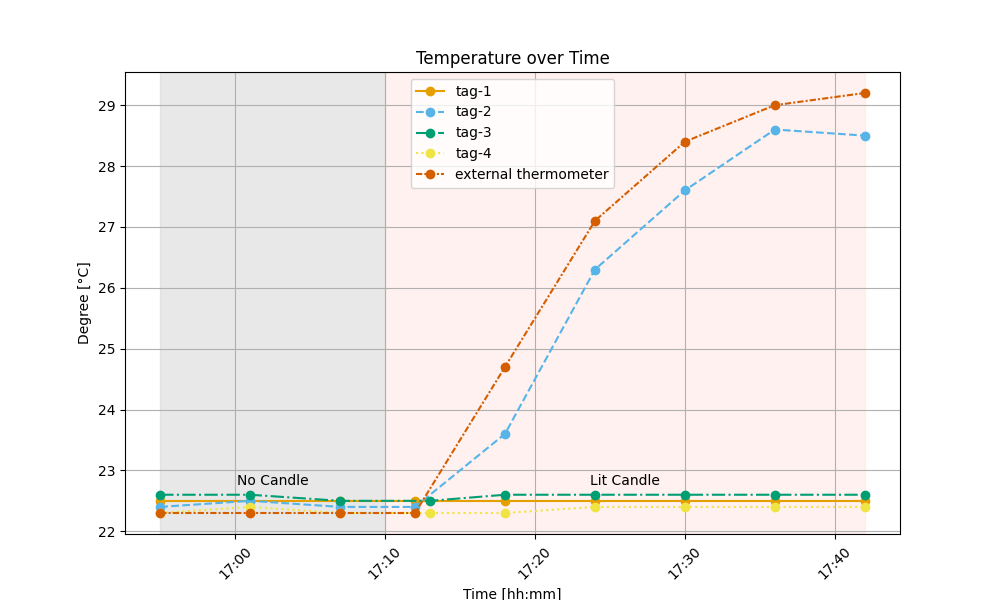
\includegraphics[width=\linewidth]{graphics/exp/exp3_temp_plot_1.png}
	\caption{Experiment 3, temperature over time, mith external measurement added.}
	\label{f:exp3_graphs_temp}
\end{figure}

The progression of the external thermoeter and the internal temperature sensor can be seen in figure \ref{f:exp3_graphs}.
The candles, that functioned as the heat source, were lit at 15.10.
The section of time before the candle was lit has a gray background.
After the candle was lit, the background becomes red.
The measurements from te external thermometor are shown with a red dashed and dotted line.
They were extracted manualy from the video. The datapoints correspond to the datapoints when Tag-2 measured.\\
Before the candle was lit, Tag-1, Tag-2, Tag-3 and Tag-4 recorded mean temperatures of 22.5\degree C, 22.4 \degree C, 22.6 \degree C and 22.3 \degree C respecivly.
The variances were all bellow 0.01\degree.
Once the candle was lit, Tag-1, Tag-3 and Tag-4 continued with similar temperature, havin mean temperatures of 22.5\degree C, 22.6\degree C and 22.4\degree C over the whole duration, with variance remaining under 0.01\degree C.


After the canle was lit, Tag-2 started to deviate from the other tags.
During the next measurement of tag 2, at 15.12, both the external thermoeter and the temperature sensor on tag 2 had not yet registered any change, remaing at 22.4 \degree C for the tag and 22.3 \degree C for the external thermometer.
The recording showed the extrenal thermometer start rising 1 minutes later, at 15.13.
During the next measurement at 15.18, the temperature-sensor registered a slightly increased temperature of 23.6 \degree C, while the external thermometer registered 24.7 \degree C.
During the next measurement at 17.24 the tag reported 26.3 \degree C while the thermometer showed 27.1 \degree C. 
The measured temperature of the external thermometer keeps klimbing faster than the temperature sensor of Tag-2, until the end of the experiment, as seen in Figure \ref{f:exp3_graphs_temp}.
The difference in measured temperature between Tag-2 and the external thermoeter nether exeeds 1 \degree C and gets smaller towards the end of the experiment, ending with a difference of 0.7 \degree C.

\begin{figure}[ht!]
	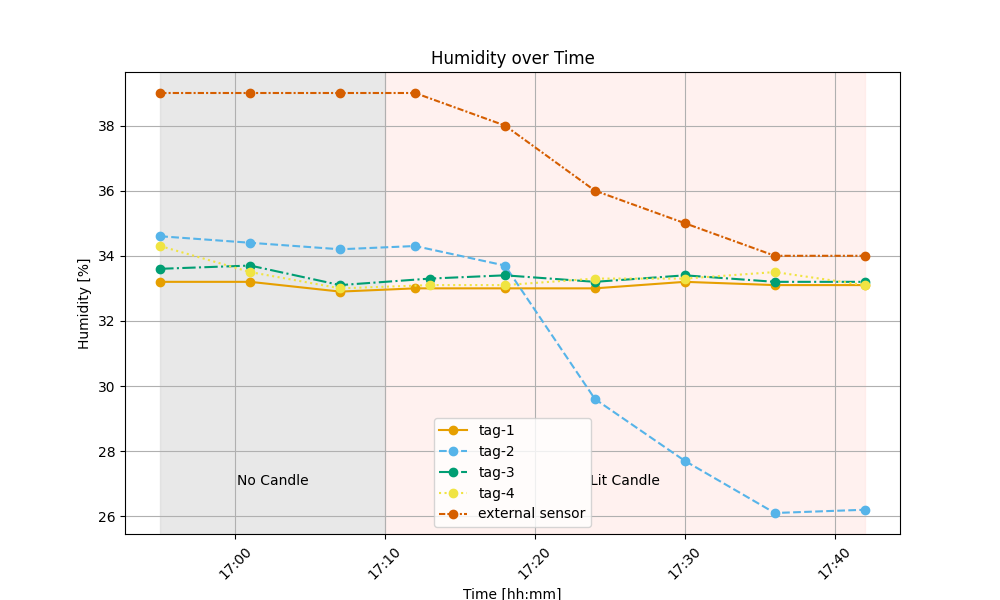
\includegraphics[width=\linewidth]{graphics/exp/exp3_hum_plot_1.png}
	\caption{Experiment 3, humidity over time, with external measurement added.}
	\label{f:exp3_graphs_hum}
\end{figure}


Experiment 3 was intended to test the temperature and not the humidity.
Luckily, the external thermoeter also included a humidity sensor, that could retroactivly be used for evaluation.
Figure \ref{f:exp3_graphs_hum} shows the humidity over time,the gray and red sections again representing the time before and after the candle was lit.
The external humidity sensor wasa added to the graph and is shown with a red dashed and dotted line.
Since the external humidity sensor was initialy not intended to be used, it is not perticulalry precise and does not display any digits after the decimal point.\\
Its values were again manual extracted from the video at the same points the times Tag-2 measured the humidity.
Tag-1, Tag-3 and Tag-4 again show a constant measurement during the experiment, having mean humidities of 33.0\% , 33.3\% and 33.4\% .
Tag 4 has the highest variance of the group, with 0.2\% , the others havin variances bellow 0.1 \%.\\
Tag-2 had a higher mean humidity of 34.4 before the candles were lit, with a variance of 0.04.
The first measurement after the candle was lit was still 34.3 \% . Afterwards the measurements started dropping, first with a small dicrease to 33.7 \% , followed by a large drop to 29.6 \%, then 22.7 \% and finally platoing at 26.2 \% .\\
The humidity sensor consitently shows a much higher humidity than the one on the tag.
When the experiment starts at 15.10, the external sensor shows a humidity of 39 \% .
It stays on this value until the candle is lit.
The first measurement after the candle is lit, at 17.12 still has a humidity of 39\% .
The external sensor than first notes a small dicline of 1\% pt, followed by a larger decline of 2\% pt to 36 \% and then decends with 1\% pt at a time until it platoes at 34\% . \\
The humdity registered by Tag-2 and the external sensor forms a similar line.
This two lines have a similar tragectory, but are not parallel.
While the difference in registerd humidity originaly is around 4.6\% pts, when both platoe, the difference has risten to 7.8\% pts.
The variance in the difference of the Tag-2 sensor and the external sensor is 2.1 \% pts over the whole measurement period.

\subsection{Conclusion}
The fact that the three sensors that are far away from the sensor don't show any sign of temperature increase was expected.
Since warm air rises, and the tags were spread more than half a meter apart, it was not expected, that the heat from the candles would reach the tags.
Even if hot air would nor rise, the energy added to the system would  be added with an efficiency of $\mathbf{O}(d^{\frac{1}{3}})$, where d is the distance.\\
The tag that is close to the candle does notice the candle with a similar speed as the external thermoetor.
The fact that it takes a while for both the external sensor as well as the sensor of Tag-2 to register the heat, has two explenations.
The first explenation is, that the external thermoetor and the DHT22 sensor are both not high precision instruments and have a natural inertia.
The second explenation is, that it takes a moment for the candles to fully burn and start heating up the air.
most likely, a combination of both factors is responsible for the delayed start.\\
The obervation that the external thermoetor registeres a higher heat than the internal sensor has two possible explenations.
It could be a difference in registered value, due to different sensor reporting different results.
It could also be, that the external sensor was actually hotter than the internal sensor.
The internal sensor was mounted on a piece of cardboard and thus shielded a bit from the heat.
The external sensor was also placed on the cardboard, but more directly exposed to the heat, sine it was placed closer to the edge of the cardboard piece.
Since initialy both sensor have very similar values, the second explenation is mire likely true.


The fact that the humidity dropped when the candles were lit should have been expected.
The \% humidity represents amount of water in the air, as a percentage of the maximal capacity of air.
The capacity of air to carry water rises with temperature.
So when the temperature rises, but no additional humidity is added, the percentage drops.
This can clearly be seen happening in this experiment to Tag-2.\\
Since the temperature around Tag-1, Tag-3 and Tag-4 does not rise, neither does the humidity fall.
This was verified by the humidity results of this experiment for those tags.\\
Tag-2 startes with a slightly increased humidity.
This is a further pointer to the theory, that the humidity of the experimenter during setup can be registered, since it took the experimenter a few minutes to set up everything around Tag-2 for experiment 2. \\
The difference in humidity between the tags and the external sensor lacks a clear explenation.
Since the humidity function is not the main purpose of the external thermometor, it is possible that it was implemented poorly, thus leading to the difference.
Further research is required to analize the precision of the DHT22 sensors.
Nethertheless, the sensor on Tag-2 shows clearly a happening thenomenon, indicating that the gerneal implementation and setup is soudn.



\section{Experiment 3: Gyroscope}
\label{s:exp_3}
Again all for tags were placed on a 80 cm by 50 cm rectangle.
Each tag was turned on sequentially and given enough time to establish the network.
The phone then was connected to one tag.
After 20 minutes one tag was turned by 90\degree clockwise.
The experiment then ran for another 30 minutes.
The goal of experiment number 4 was to test the detection of unwanted rotations.


Experiment 3 was performed in two differing manners.
The orirentational read was originaly the only implementation for the gyroscope.
After experiments one to four were evaluated, the lack of usefull results from the gyroscope readings prompted a redesign of the sensor.
This resulted in the development and implementaiton of the angular velocity read.
Experiment 3 was repeated with the angular velocity read of the gyro.\\
For the orientational read, the maximal allowed angular difference was set to 30\degree.
For the angular velocity read, the maximal allowed angular velocity was set to 100 $\frac{\deg}{s}$.
The results for the orientational and the angular velocity read will be presented seperatly. The conclusion will talk about them both.


\begin{figure}[ht!]
	\centering
	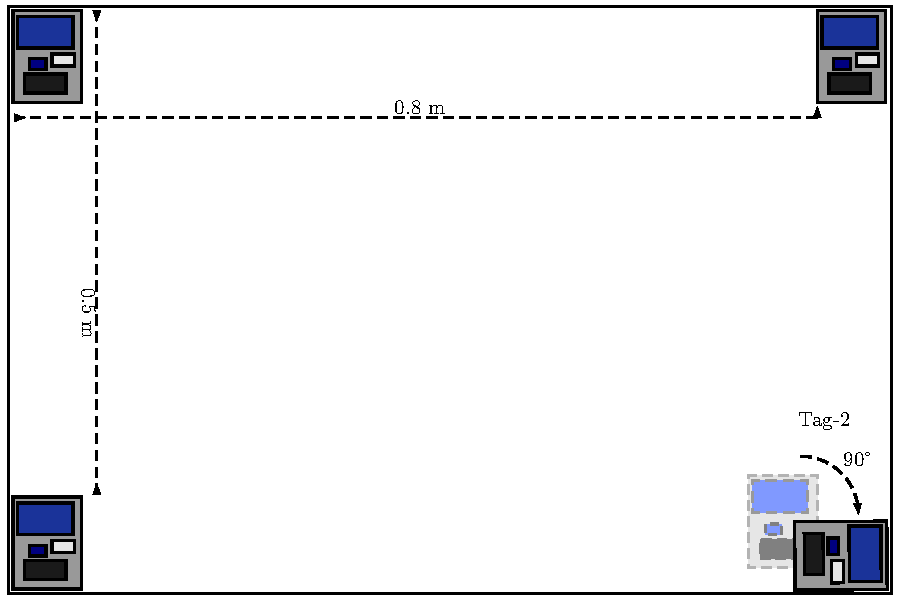
\includegraphics[width=300px]{graphics/schematics/experiment_3.pdf}
	\caption{Schema of the setup of experiment 3.}
	\label{f:exp3_schematic}
\end{figure}


\subsection{Reults orientational read}
\label{ss:exp_3_result}
Experiment 3 was intended to check the functionality of the gyroscope.
Temperature and humidity behaviour were the same as in the static experiment \ref{ss:exp_1_result}.
As already seen during the evaluation of experiment 1, the gyroscope does not work as planned.


Figure \ref{f:exp4_graphs_gyro} shows the values of the gyro over time.
Tag 1 was rotated by 90\degree  at 22.25 around the Z axis.
The gray section marks the park of the experiment beofre the turn, while the red shows the results after the turn. \\
Tag-3 has a mean of 0 and 0 variance of 0 during the whole experiment for axes X and Y.
Tag-4 has one measurement that has 0 mean and variance as well, at axes Y.
Their is no disernable change in the output of the gyro during or after this process in any of these measurements. \\
Some other orientation are also manly zero during this experiment.
The orientation of the Z-Axis of Tag-3 is zero for six out of the eight performed measurements, only spiking once at the beginning for two reads.
The other axes of Tag-1 have values 100\degree and 290\degree at the beginning and then stay zero for the rest of the experiment.
The Y and Z axis of Tag-2 are also zero for almost all measurements except for one measurement at 22:11, where they registered an orientation of 235\degree and 5\degree respecivly
This is escpecially unescpected, since Tag-2 was the one who was turned around axis Z. \\
Axis z of Tag-1 forms zig-tag line between values from 25\degree to 100 \degree and 200 \degree to 300 \degree.
Tag-4 axis X and Z and Tag-2 Axis X follow no decernable pattern.


\begin{figure}[ht!]
	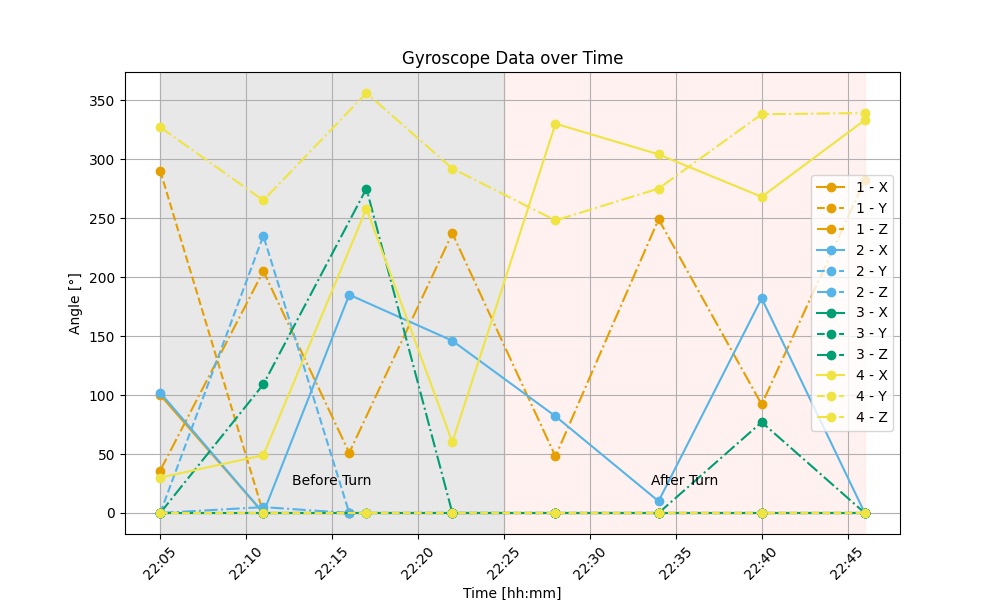
\includegraphics[width=\linewidth]{graphics/exp/exp4_gyro_data_plot_1.png}
	\caption{Experiment 4, gyroscope over time.}
	\label{f:exp4_graphs_gyro}
\end{figure}

Figure \ref{f:exp4_graphs_dist} shows the distances over time for pairs, as discussed in section \ref{ss:exp_1_result}.
Before the event, all measured distances are stable, except for one outlier in the distance 1=2.
As in experiment 1 \ref{ss:exp_1_result} the distances are not equivalent with the physical distances in the experiment.\\
After the tag is turned at 22.26, all measurements involving Tag-2 change and then remain at the new distance.
Distance 1=2 dicreases from 0.71 m to 0.42, after a short jump to 1.4m.
Distance 2=3 is on 0.92 before the measurement and 1.11m afterwards. It is also involved in a measurement during the turn, measuring 0.65m.
Distance 2=4 is originaly at 0.65m before the turn and ends up at 1.10m afterwards.
The other pairs, 1=3, 1=4 and 3=4 don't change values siginificantly during this time, having variances of 0.001, 0.004 and 0.000 respectifly.

\begin{figure}[ht!]
	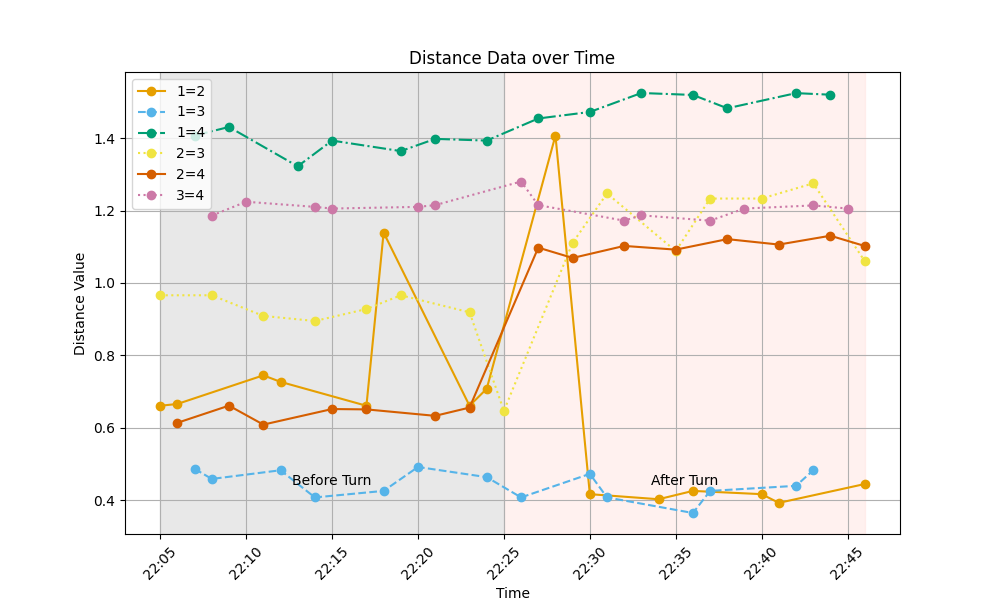
\includegraphics[width=\linewidth]{graphics/exp/exp4_dist_data_plot_1.png}
	\caption{Experiment 3, gyroscope over time.}
	\label{f:exp4_graphs_dist}
\end{figure}


\subsection{Results angular velocity read}
\label{ss:exp_3_result}
As with the orientational read, this experiment had no results that differed from the static experiment, when analyzing temperature and humidity.
The experiment was started at 10:01 and was terminated 10.40.
Tag 2 was turned at 10.18 by 90\degree around the Y axis by hand.
Figure \ref{f:exp4_graphs_gyro_2} shows the angualr velocity of all tags during the experiment.
The angular velocity of tag i around axis v will be labeled as $a_i^v$.
All axises of Tag-2 are shown in blue, with the angular velocity around the X axis, $a_1^X$ ,beeing a filled line, around the Y-Axis a dashed line and around the Z axis beeing dashed and dotted.
The Y axis of figure\ref{f:exp4_graphs_gyro_2} is displayed using a log-scale, to better show the low values.
The time before the utrn has a gray backgroudn, while the time after the turn is displayed with a red background.


Tag-2 has constant angular velocity for all three measurements before the turn.
$a_2^X$ is $12\frac{\degreem}{s}$, $a_2^Y$ is between $14\frac{\degreem}{s}$ and $17\frac{\degreem}{s}$  and $a_2^Z$ is a constant $20\frac{\degreem}{s}$ before the turn.
The first measurement after the turn reports angular velocities of $445\frac{\degreem}{s}$, $6322\frac{\degreem}{s}$ and $716\frac{\degreem}{s}$ for axis X,Y and Z of Tag-2.
Afterwards the values return back to their original values.
$a_2^X$ is $13\frac{\degreem}{s}$, $a_2^Y$ is $14\frac{\degreem}{s}$ and $a_2^Z$ $20\frac{\degreem}{s}$, all constant measurements, after the turn.

\begin{figure}[ht!]
	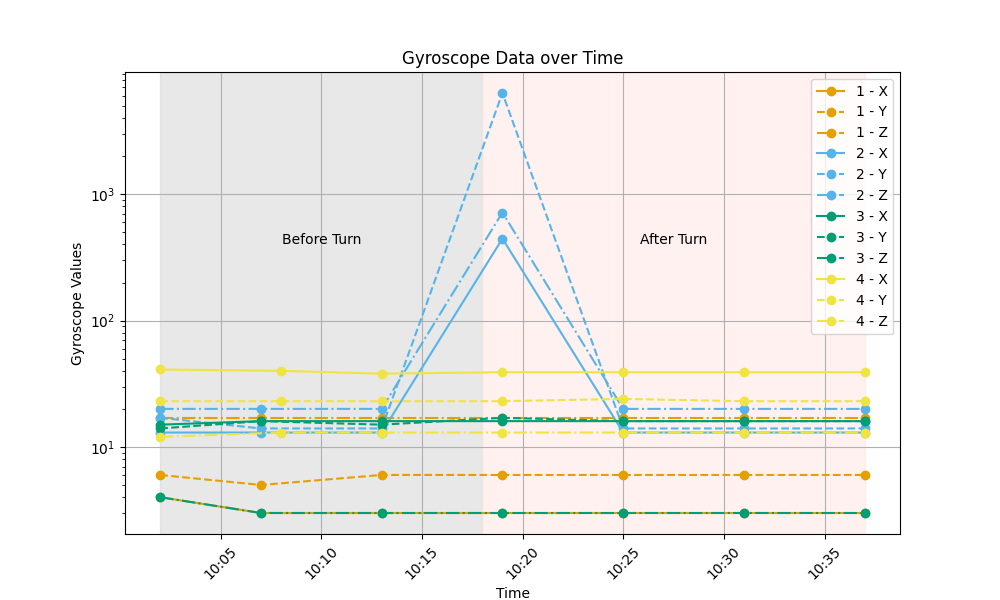
\includegraphics[width=\linewidth]{graphics/exp/exp4_2_gyro_data_plot_2.png}
	\caption{Experiment 3, gyroscope over time, using the angular velocity read.}
	\label{f:exp4_graphs_gyro_2}
\end{figure}

Tag-1, Tag-3 and Tag-4 are in orange, green and yellow respectivly.
They all keep a measurements with minimal fluctuation.
Table \ref{tab:gyro_mean_2} shows the mean values and variances of all tags and all axes.
Tags-1 has no variance that exceeds 0.143, with $a_1^Z$ even showing a constant value over all seven measurements, leading to a variance of zero.
Tag-3 and Tag-4 both have two axes with variances of 0.143 and one axis with a variance of 0.905.
The mean values of Tag-1, Tag-3 and Tag-4 are in the reange of $3\frac{\degreem}{s}$ and $40\frac{\degreem}{s}$, with five falling into the range of $15\frac{\degreem}{s}$ to $25\frac{\degreem}{s}$.
Tag-2 has variances between 740 and 16128.

\begin{table}[h!]
\centering
\caption{Summary of Gyroscope Data: Means and Variances of X, Y, Z Axes}
\begin{tabular}{c|c c c|c c c|}
\hline
\textbf{tag} & \textbf{mean x} & \textbf{mean y} & \textbf{mean z} & \textbf{var x} & \textbf{var y} & \textbf{var z} \\
\hline
\textbf{tag-1} & 3.143 & 5.857 & 17.000 & 0.143 & 0.143 & 0.000 \\
\textbf{tag-2} & 23.3 & 41.3 & 68.0 & 741 & 5024 & 16128 \\
\textbf{tag-3} & 15.857 & 15.714 & 3.143 & 0.143 & 0.905 & 0.143 \\
\textbf{tag-4} & 39.286 & 23.143 & 12.857 & 0.905 & 0.143 & 0.143 \\
\hline
\end{tabular}
\label{tab:gyro_mean_2}
\end{table}


Figure \ref{f:exp4_graphs_dist_comb_2} shows the pairs of ditances over time of experiment 3 using angualr velocity read.
The distances 1=2, 1=3, 1=4, 2=3 and 2=4 stay in a similar range over the whole experiment.
Table \ref{tab:exp4_var_distanc} shows the mean and variance of the combined distance measurements.
The variance in measured distances 1=2, 1=3, 1=4, 2=3 and 2=4  are all below one milimeter.
The measured distances are between 0.39m and 0.87m.
The measured distance 3-4 behaves very differently.
It is bigger than all others, with 1.18m.
It also has a comperatavly high variance of 0.05m.
Its lowest measurement is the first measurement after the turn.
Looking at the split distance-measurement 3-4 in figure \ref{f:exp4_graphs_dist_split_3_4} shows, that the change in distance comes mainly from the measurements originating from tag 3.
Distance measurements from Tag-3 to Tag-4 have a variance of 0.074m, while measurements from Tag-4 to Tag-3 have a variance of 0.014m.

\begin{figure}[ht!]
	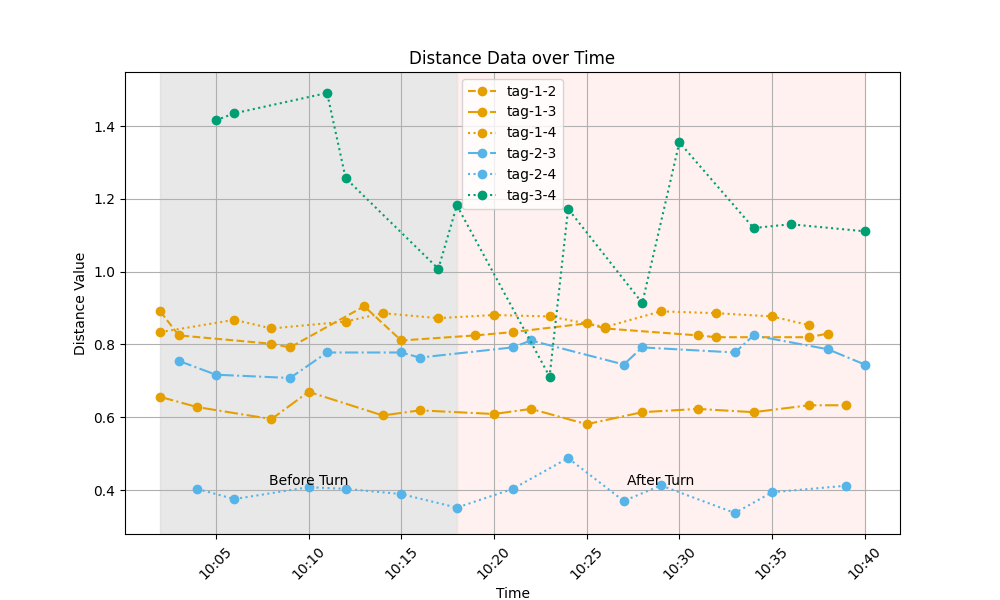
\includegraphics[width=\linewidth]{graphics/exp/exp4_2_dist_combined_2.png}
	\caption{Experiment 3, combined distance over time, using angular velocity read.}
	\label{f:exp4_graphs_dist_comb_2}
\end{figure}

\begin{table}[ht]
\centering
\caption{Statistics of the combined distance measurements between tags for experiment 3 with angular velocity read}
\begin{minipage}{0.45\textwidth}
\centering
\begin{tabular}{|c|c c c|}
\hline
  & 2 & 3 & 4 \\
\hline
1    & 0.0.834 & 0.622 & 0.868 \\
2   &  & 0.770 & 0.396 \\
3   &  &  & 1.177 \\
\hline
\end{tabular}
\caption*{Mean}
\end{minipage}
\hfill
\begin{minipage}{0.45\textwidth}
\centering
\begin{tabular}{|c|c c c|}
\hline
  & 2 & 3 & 4 \\
\hline
1    & 0.001 & 0.001 & 0.000 \\
2   &  & 0.001 & 0.001 \\
3   &  &  & 0.049 \\
\hline
\end{tabular}
\caption*{Variance}
\end{minipage}
\label{tab:exp4_var_distanc}
\end{table}

\begin{figure}[ht!]
	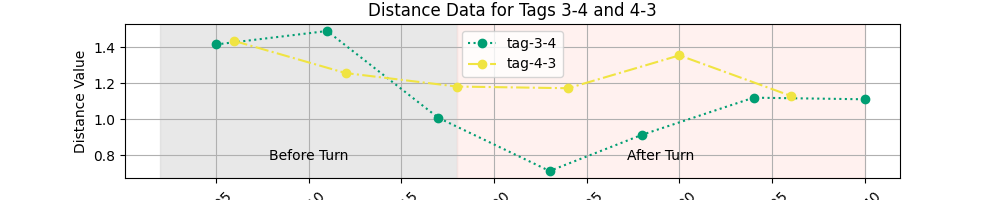
\includegraphics[width=\linewidth]{graphics/exp/exp4_2_gyro_split_distance_3_4.png}
	\caption{Experiment 3, split distance measurement between Tag-3 and Tag-4 over time.}
	\label{f:exp4_graphs_dist_split_3_4}
\end{figure}

\subsection{Colclusion}
\label{s:exp_3_conclusion}
The orientational read of the gyroscope produces puzzeling rezluts.
Many values are zero for most of the time, but not consistently.
This does not make any sense, since the orientational read does not reset after it has been read, rather it updates continously.
For a measurement to reutrn to zero after a wrong value, it would need to make the exact same mistake again in reverse.
This seems highly unlikely, escpecialy for it to happen four times in one experiment.
Additionaly, the one orientation that should change, because it was physically turned, remains at zero before and after the turn.
The most plausible explenation for this behaviour is, that their is an error in the implementation of the gyrosscope module when performing read.
Errors that could lead to such behaviour would be, if the orientational values could reset at runtime or if the wrong values are returned when queried.


The angular velocity read on the other hand produces usefull results.
The turn of tag 2 is very visible, while the other tags remain unaffected.
The angular velocity aaround the X axis for Tag-2 reaches a maximal value of 6322 during this reading.
While this might seem like a high value, it would mean that the turning of the tag, if performed at maximum speed constantly, would have taken 0.05s.
Taking into account that this was a maximum speed and that a human can turn something quite fast, this seems like a reasonable result.\\
Axis Y and Z show a rotational high velocity as well, even it is still smaller by a factor of ten than the rotation around the X-Axis.
Since the sensor was attached on the cardboard by zip ties, it would have had some room to move during the turn.
Additionaly since the turn was performed by hand, it is reasonable to assume, that it was not performed perfectly around the X-axis.
These to effects in combination could account for the high angular velocities around the unaffected Axis.
These results show, that the angular read can be used to detect rotational movement on the Tag. \\
In addition we get an estimate for the biases of the MPU6050.
It appears that the sensor outputs an angular velocity between $0\frac{\degreem}{s}$ and 50 $0\frac{\degreem}{s}$.
While this does not explain the result for the orientational read by itself, it may inform those readings.

During the orientational experiment, the Tag was turned around the Z-Axis, with an atempt beeing made to keep the MPU6050 sensor in the center.
This moved the antenna of the DWM3000 board closer to the tag 1 and further away from Tag-3 and Tag-4.
This behaviour was captured by the distance measurements.
While the distance values are still not correct, even the differences, it caputes something that actually happened in during the experiment.\\
Since the results of the oritentational read were already known during the angular velocity read experiment, a descision was made to test, if a better turn could prevent the distance read.
Instead of the Z-axis, the X-Axis was chosen for the turn, since it corresponds to the antenna position of the DWM3000 baord.
Additionaly the turn was centered around the DWM3000 shield instead of the MPU6050.
This results in the turn not beeing visible in the distance reads from the experiment.\\
It is unclear why the distance measurements between Tag-3 and Tag-4 were inconsisten, when originating with Tag-3. 
Both tags were not part of the experiment.
If a repeated multipath-effect would appear, it should affect both mesurments euqaly, since both participate in DS-TWR.
Tag-4 served as the connection to the Phone in this experiment.
It is possible, that a poor interaction between the BLE and UWB systems happened.
It would be surprising, that these errors only appeared, when Tag-4 was participating, but not initiating the ranging session.


\section{Experiment 4: Distance}
\label{ss:exp_4}
The same 80 cm by 50 cm rectangle setup was used as in previous experiments.
The tags were turned on sequentilay, giving them enough time to build the network.
The phone was connected to one tag.
The max distance parameter was set to 20 centimeter.
After 20 minutes, Tag-1 was moved parallel to the shorter rectangle line about 20 cm towards Tag-2 on the next corner.
Figure \ref{f:exp4_schematic} shows a schemativ view of the experiment.
The system was then left resting for another 30 minutes.
The goal of experiment 4 was to test the detection of unwanted movement.


\begin{figure}[ht!]
	\centering
	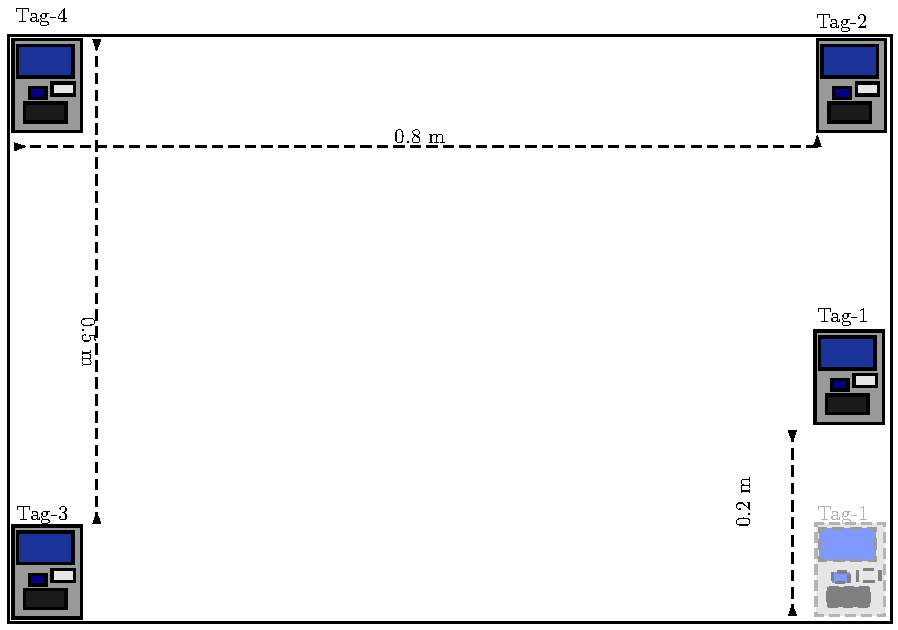
\includegraphics[width=300px]{graphics/schematics/experiment_4.pdf}
	\caption{Schema of the setup of experiment 4.}
	\label{f:exp4_schematic}
\end{figure}

\subsection{Results}
\label{ss:exp_4_result}

Experiment four was intended to test the distance measurement capabilities of the setup.
Temperature and humidity and gyro behave as they do in experiment 1 \ref{ss:exp_1_result}.
For the gyroscopic data, the orientational read was used.
It presents the same issues as in experiment 1 and 3.
Humdity, Temperature adn Gyroscope will not be discussed further for tis experiment.

\begin{figure}[ht!]
	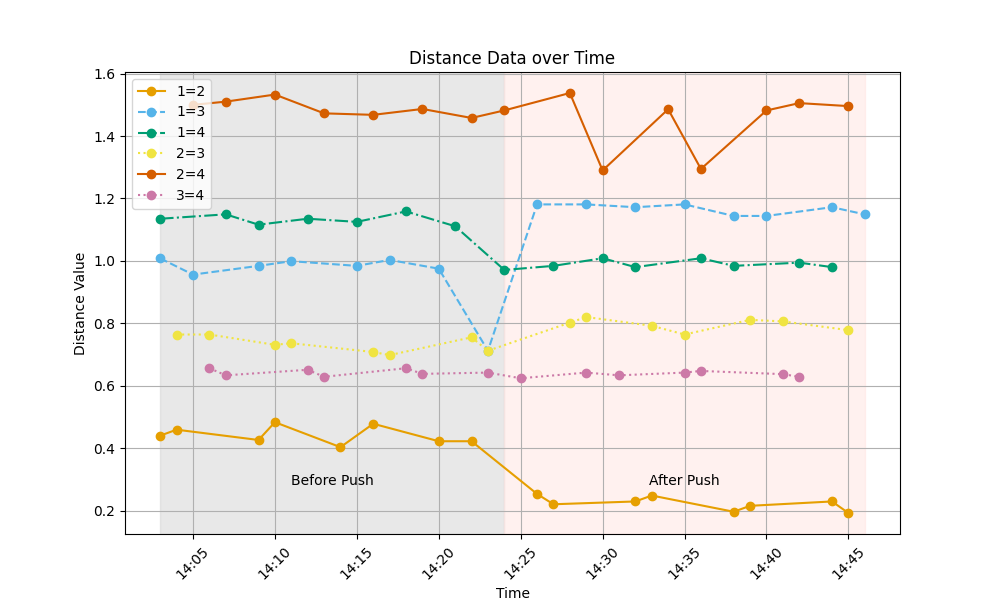
\includegraphics[width=\linewidth]{graphics/exp/exp5_dist_data_plot_2_combined.png}
	\caption{Experiment 4, pairs of distance over time.}
	\label{f:exp3_graphs_dist}
\end{figure}


As with previous distance measurements, the pairs of distances moved together.
Figure \ref{f:exp5_graphs_dist} shows the measured distance pairs of the 4 tags over time.
At 14.24 Tag-1 was moved by 0.23 meters toward Tag-2.
The time before the push has a gray background, while the time after the push has red one.
The measured distances from Tag-1 to Tag-3 increases, while the distance to Tags-2 and Tag-4 dicreases.
This represent what is happening in reality, since Tag-1 is now closer to Tag-2 and Tag-4 and further away from Tag-3 as before.

\begin{figure}[ht!]
	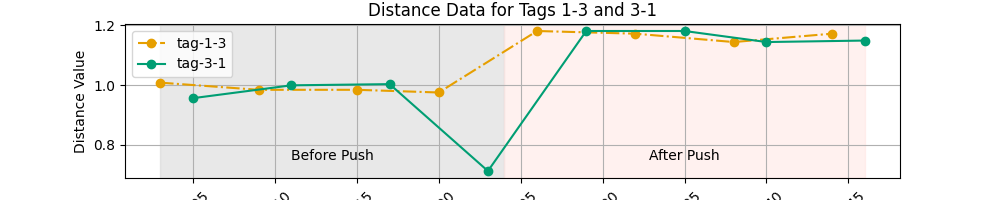
\includegraphics[width=\linewidth]{graphics/exp/exp5_dist_data_plot_2_split_1_3.png}
	\caption{Experiment 4, distance between Tag-1 and Tag-3}
	\label{f:exp3_graphs_dist_split_1_3}
\end{figure}


Table \ref{tab:exp4_mean_distances} shows the mean values of distance pairs before and after the move.
The variances for all values, are low, confirming the choice to combine pairs during evaluation.
As in experiment 1 and 3, the reported distances do not correspond to the what is phisically happending.
The difference in mean distance 1=2 before and after the push is 0.209m.
This is close to the 0.23m that Tag-1 was acutally moved to Tag-2.
The measurements show Tag-4 0.144m closer to Tag-1 after the push.
The effect on tag 4 should be notissable but not as large as it is.
Since the tag moves lateraly towards tag 4, the difference should only be 0.03 meters.
The difference in measured distance between Tag-1 and Tag-3 is 0.213 meters.
Figure \ref{f:exp3_graphs_dist_split_1_3} shows the distance measurements between Tag-1 and Tag-3.
Measurement 1-3 and 3-1 move together as a pair, ecepct for the fourth measurement of distance 3-1.
This also shows the higher variance of pair 1=3.
If the outlier value is ignored, the distance difference between the means beofre and after the oush becomes 0.179 meters. 
This is still too large for the difference a latteral move, it should only be a 0.100 m difference.
Their is also a small increase in the distance between tags 2 and 3, but which starts before tag 1 was moved.


\begin{table}[ht]
\centering
\caption{Statistics of the combined distance measurements between tags before and after the push for experiment 4}
\begin{minipage}{0.45\textwidth}
\centering
\begin{tabular}{|c|c c c|}
\hline
		& \textbf{Tag-2} & \textbf{Tag-3} & \textbf{Tag-4} \\
\hline
\textbf{Tag-1}    & 0.442 & 0.953 & 1.133 \\
\textbf{Tag-2}   &  & 0.734 & 1.490 \\
\textbf{Tag-3}   &  &  & 0.654 \\
\hline
\end{tabular}
\caption*{Mean before move}
\end{minipage}
\hfill
\begin{minipage}{0.45\textwidth}
\centering
\begin{tabular}{|c|c c c|}
\hline
		& \textbf{Tag-2} & \textbf{Tag-3} & \textbf{Tag-4} \\
\hline
\textbf{Tag-1}    & 0.223 & 1.166 & 0.989 \\
\textbf{Tag-2}   &  & 0.796 & 1.447 \\
\textbf{Tag-3}   &  &  & 0.635 \\
\hline
\end{tabular}
\caption*{Mean afer move}
\end{minipage}
\hfill
\begin{minipage}{0.45\textwidth}
\centering
\begin{tabular}{|c|c c c|}
\hline
		& \textbf{Tag-2} & \textbf{Tag-3} & \textbf{Tag-4} \\
\hline
\textbf{Tag-1}    & 0.000 & 0.010 & 0.000 \\
\textbf{Tag-2}   &  & 0.001 & 0.001 \\
\textbf{Tag-3}   &  &  & 0.000 \\
\hline
\end{tabular}
\caption*{Variance before move}
\end{minipage}
\hfill
\begin{minipage}{0.45\textwidth}
\centering
\begin{tabular}{|c|c c c|}
\hline
		& \textbf{Tag-2} & \textbf{Tag-3} & \textbf{Tag-4} \\
\hline
\textbf{Tag-1}    & 0.000 & 0.000 & 0.000 \\
\textbf{Tag-2}   &  & 0.000 & 0.010 \\
\textbf{Tag-3}   &  &  & 0.000 \\
\hline
\end{tabular}
\caption*{Variance afer move}
\end{minipage}
\label{tab:exp4_mean_distances}
\end{table}

\subsection{Conclusion}
\label{s:exp_4_conclusion}
As was shown in Experiment 1, the distances do not match with the phsiscal distances.
However, the differences in distance materialize correctly.
The correct distances increase and dicrease to match the physical reality.
The most probable reason for the incorrect distances is the simplified calibration.
The difference between the correct and measured distances never exeeds 0.4m, which is the assumed error by Qorvo, when using incorrect calibration.\\
The difference in distance is even closer, onyl beeing off by 0.1m at most.
For now this error is still too large to be used unmodified in real world applications.


\section{Experiment 5: Real World experiment}
\label{s:exp_5_real_world}
Experiment 5 was designed to check, how the setup would do in a real world applicaion.
For this, all tags were put in a rucksack and taken on a journey.
To protect the electronics from damage, each tag was put in a transparent cylindrical plastic bucket with radiu 012m and a hight of 0.14m and no lid.
The buckets in the rucksack were stacked so there were two next to each other at the bottom and two on top.\\
First, the rucksack was taken by foot from Binzmmühlstrasse 14 by foot to the Zurich Oerlokon train staiton.
From their the journey continued via train to Zurich Main Station.
After a short walk in Zurich Main Station, the journey continued via train to Lenzburg, were the jouney ended at the Lenzburg train station. \\
During the whole journey, the backpack was on the back of the person conductung the experiment and was nether put on the floor.
This was done to protect the electronics from potential accidents by careless travelers during rush-hour.

\subsection{Results}
\label{s:exp5_real_worl_results}
The walk by foot began at 17.43 and ended 17:51 when the S6 train to the main station was entered.
The S6 arrived at the main station at 18:01.
From their the track had to be changed and 18.08 the train to Lenzburg was entered.
The train drove for 24 minutes, until the experiment ended 18:32 at the Lenzburg trainstation.\\
The following section will contain Figures for this journey.
The figure all use the same color scheme to describe the journey.
The first part by foot will have a gray background.
The first trinride in the S6 will have a red background.
The time in Zurich Main Station is blue and the final trainride to Lenzburg green.

\begin{figure}[ht!]
	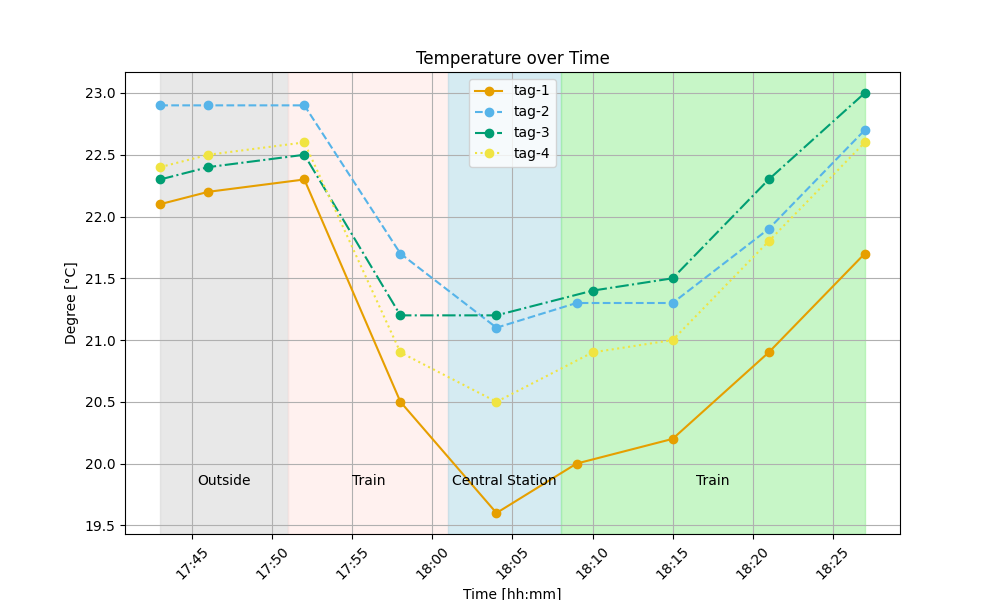
\includegraphics[width=\linewidth]{graphics/exp/exp6_temp_plot_2.png}
	\caption{Temperature over time during experiment 5.}
	\label{f:ex5_train_temp}
\end{figure}

Figure \ref{f:ex5_train_temp} shows the measured temperatures during experiment 5.
All four tags start with a high temperature between 22\degree and 23\degree .
This remains true until the train is reached, were the temperatures start drop during the second measurement in the train to by a bit over one degree to a range of 20.5\degree to 21.7\degree .
During the one measurement in the main station, most tags have their lowset values during the whole experiment, Tag-1 with 19.6\degree , Tag-2 with 21.1\degree and Tag-4 with 20.5\degree .
The only tag without a significant drop during the main station is Tag-3, which records the same temperature of 21.2\degree as in the previous train.
During the second train ride, all tags report a stadely increasing temperature. \\
Tag-2 starts with the a temperature that is 0.5\degree higher than the other tags, who all start with very close values.
Tag-1, Tag-3 and Tag-4 stay close until the first train ride.
From there on Tag-1 drops to lower temperature measurements that are 1\degree lower than the lowest measurement of the rest, Tag-4, and stays there until the rest of the experiment.
Tag-2 and Tag-3 report similar values during the Main Station and keep having similar values until the end.
Tag-4 reports values that are close to Tag-2 and Tag-3, but alwys below it. This becomes specialy pronounced at the main station, where Tag-4 measures 20.5\degree , 0.6 \degree lower than Tag-2 and 0.7 \degree lower than Tag-3.




\begin{figure}[ht!]
	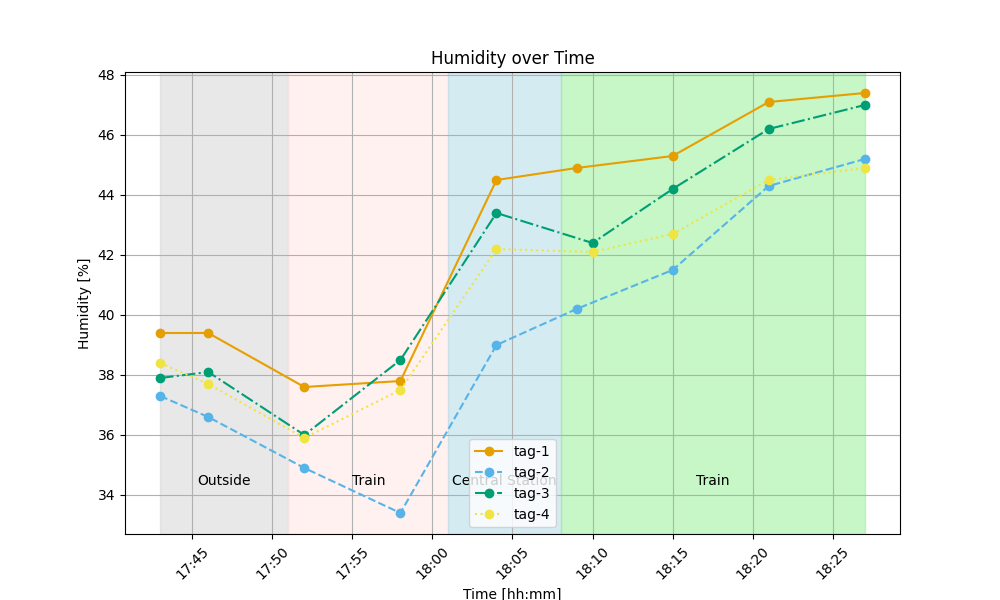
\includegraphics[width=\linewidth]{graphics/exp/exp6_hum_plot_2.png}
	\caption{Humidity over time during experiment 5.}
	\label{f:ex5_train_hum}
\end{figure}
%\chapter{Final Considerations}
\label{chap:considerations}

This chapter provides a summary of this thesis \ref{s:sumary}, a conclusion of what was achieved \ref{s:Conclusion} and it lays out future work that could be build on this thesis \ref{s:future_work}.
The goal of this is to provide a wrap-up of this thesis.

\section{Summary}
\label{s:sumary}

This thesis introduced a design for a wireless sensor network (WSN) to monitor artworks during transportation and inform the driver about the status of his load.
This involved the tag beeing equiped with temperature and humidity sensors and a gyroscope, as well as peripherals for UWB and BLE communications.
The tags would build a peer to peer network using UWB, that a phone could connect to using BLE.
The phone would run an app that queries the WSN for measurements and presents the result to the driver.
Based on parameters provided by the driver, the app would warn the driver about measurements that indicate a problem.
Next to sensor data, the provided system also included distance data between the tags, gathered by using UWB two-way ranging.
The App builds a working model of the positions of the tags based on this data.


In a first step, theoretical knowledge about relevant field was gathered.
This thesis provides a sumary on the relevant parts in the fields of: Wireless sensory Networks, Ultra wideband, Two-Way ranging and k-connected graphs (TODO: Liste erweitern wenn mer dazu kommt!).
Additionaly the current state of research in related fields was presented, consisting of: Artwork Tracking, sensor networks and wireless ranging.


The system design includes a description of the hardware used, including a breakdown of the tag components. It descirbes the way all hardware components communicate with each other and how to connect them correctly.
It then provides the architecture of the system, describing the different modules used and what theor individual services and responsibilities are.
A detailed description of how data flows through the system was provided.
Lastly the network architecture was provided, describing how tag join and communicate. The thsis showed how this implementation ensures, that a unique model of the tag positions in the system can be calculated, and how this model is calculated efficiently.


The implementation followed the outlined system design, using a nRF52840 microcontroler, the DHT22 temperature and humidity sensor, the MPU6050 gyroscope, DWT3000 UWB shield and an Adnroid phone.
The implementation descibes how each sensor was initiated and operated.
It describes how the UWB network was build, how UWB two-way ranging was implemented and how a BLE connection is established.
It shows how all parts of the system are coordinated and the steps needed to run them all on the same system.
Lastly the process of developing the app and how it is operated by the user is described.


The system was evaluated, by performing five experiments and evaluating the gathered results. 
The first experiment tested a static system, with no changes to the tags. 
The second introduced heat to one of the tags, testing if the workings of the heat and humidity sensors.
The third tested the functionality of the gyroscope and involved turning one the the tags around itself after a period of rest.
The fourth experiment tested the ranging capabilities of the tag and consistet of moving the tag around.
The fith ecperiment checked how the system would behave outisde of the laboratory environment. The tags were taken on a journey that envolved walking and taking trains.

\section{Conclusions}
\label{s:Conclusion}

A comprehensive exploration of the current standing of sensory networks for the monitoring of artworks has been conducted, giving insight into the use of IoT devices and wireless sensory networks in this field.
A design was presented that would allow for the tracking of artworks during transportation in a truck, using different sensors and distance measurements.
The provided design was sucesfully implemented and tested.


The testing showed that the developed system is capable of querying data from the tags and reporting it.
The system can run for an extended amount of time unsuperwised and reports problematic data correctly to the user via phone.\\
The results from temperature and humidity measurements showed, that these measurements are working in the systems as intended.
The temperature data showed readings that were consistent with other devices and were consisten betwen the tags with up to one degree.
The humidity readings were mostly consosten between the tags but differed from external sensors by a larger margin.\\
The reading of the gyroscope had to be implemented two times.
An atempt to track the current orientation of the tag using the gyroscope readings showed inconsistent data.
Tracking the maximal angular velocity captured since the last measurement was fruitfull and provided usefull insights into the movement of the tag.\\
The distance measurements showed readings that did not correspond to the distances in the physical world.
Nethertheless, the readings were consistent and the difference in distance between event mirrored what happend en the event.
The distance measurements are currently not precise enough to build a tag positioning systems, but they can be used to detect unwanted movement between the tags.


Overall the design was sucesfull and shows that a artwork tracking system using these fundamentals could be used.
The selection of the sensors that are most sutable for the system still needs to be developed.
The distance measurement needs to be improved.
These are both potental research topics for future work.

\section{Future Work}
\label{s:future_work}

The implementation used in this thesis was intended as a proof of concept and therefore does not implement a fully functional art-tracking system.
A focus was put on different types of sensors and how they would interact and report to the system.
Therefore the focus was not on choosing the optimal sensors for an art-tracking system.
Future work could focus on the types of sensors used and assure they are optimaly chosen to capture all aspects that are relevant during art-preservation.
This research could include, but is not limited to:
\begin{itemize}
	\item The inclusion of a light-tracking sensor
	\item Compare different humidity and temperature sensors.
	\item Use gyroscopic data and ascelerometers to detect problematic vibration during travel, similar to \cite{landi2022iot}
\end{itemize}


The distance measrement and evaluation is not fully actulaized in this implementation.
Future research could improve on the implementation by developing a better calibration method, then used in this implementation.
This would presumably involve building the calibration system proposed by Qorovo. \\
With better distance measurement, future researchers could implement the positioning model proposed in the design section of this thesis. 
This would include small ajustment to the network building of the tags, and adding the functionality to the phone to build and solve the quadratic program.\\
A better distance measurement would also allow for a better handeling of outliers and currupted data. As described in the limitations section of the evaluation \ref{s:chalanges}, the measurements from nearby nodes could be used to handle this kind of behaviour.


The experiments were performed with only four tags and without access to an actual truck.
It would be interesting to test the implementation on a larger scale, envolving more tags and differing modes of transportation.
Research like that could investigate, if the design is well suited for real world use.

Finaly the system could be addapted for systems other than trucks.
The general design of the wireless sensor network could remain the same, even when transporting on a train or airplane.
The communication with the phone would need to be adapted.
BLE does not have infinite range and the presence of solid barriers shortens its distance even more, especialy metal ones.
So a new design to communicate between the respoinsible person and the sensor network would be required.

%\chapter{Fundamentals}

\section{Background}


\subsection{Ultra Wideband}

\subsubsection{IEEE}

The Ultra Wideband (UWB) communication protocoll was introduced in 2003 by the Institute of Electrical and Electronics Engineers (IEEE) as part of the IEEE 802.15.4 standard.
In 2020 updates were made to the protocoll when the IEEE 802.15.4z-2020 standard made improvements to the PHY layers of UWB connections. %“IEEE standard for low-rate wireless networks–amendment 1: Enhanced ultra wideband (UWB) physical layers (PHYs) and associated ranging techniques,” IEEE, C/LM - LAN/MAN Standards Committee, 2020
It achieved this by introducing a more robust timestamping system on the PHY layer.
This is suplemented by changes to the MAC layer, that allow for the exchange of ranging information.
The result is short frames, that are transmitted fast, between devices, leading to short bursts of communications that are fast, secure and ideal for ranging.


UWB works by using short radio frequency pulses, resulting in a large bandwidth.
UWB is a lower power communication form.
This prevents it from interfering with other communication forms it is sharing its wavelength with, such as WLAN or Bluetooth. 
Since UWB uses very short, distinc pulses over a short range, it has found use in ranging systems. %E. Hsu, “An overview of the IEEE 802.15.4 HRP UWB standard.” https:// blogs.keysight.com/ blogs/ tech/ rfmw.entry.html/ 2021/ 07/ 28/ an overview of IEEE-J7ac.html , 2021. (Accessed: 2022-12-22).
UWB is split into high rate pulse (HRP) UWB and low rate pulse (LRP) UWB.
Since ranging is part of this work and LRP is generally not used for ranging, I will not discuss it further in this thesis. %E. Hsu, “An overview of the IEEE 802.15.4 HRP UWB standard.” https:// blogs.keysight.com/ blogs/ tech/ rfmw.entry.html/ 2021/ 07/ 28/ an overview of IEEE-J7ac.html , 2021. (Accessed: 2022-12-22).
Since UWB devices tend to be small and have a low energy consumption, in combination with the capability of ranging as well as data transfer, they have become popular as Internet of Things (IoT) devices. \\ 

The standard defines the PHY and MAC layer as well as frequency bands for communication.
The 4z expansion tries to integrate UWB into the the WPAN standard. In Section ... and ... I will discuss the PHY and MAC layer.\\

The sending devices emits pulses in a pre-set band of frequencies, using short bursts to transmit the bits.
The signal forms a concave curve in this band, where the two points that are 10 db below the maximum power spectral density are called the lower- and upper-frequency point, see Figure \ref{f:UWB_spectrum}.
These two points must at least 500 Hz apart.
The maximum power spectral density must be below the noise level.
This process prevents conflicts with other communications, that use a single frequency with a high power spectral density and modulate signal transmission, such as WI-FI or Bluetooth.
The UWB protocol has the added benefit of being useful for high accuracy localization.


\begin{figure}[ht!]
\centering
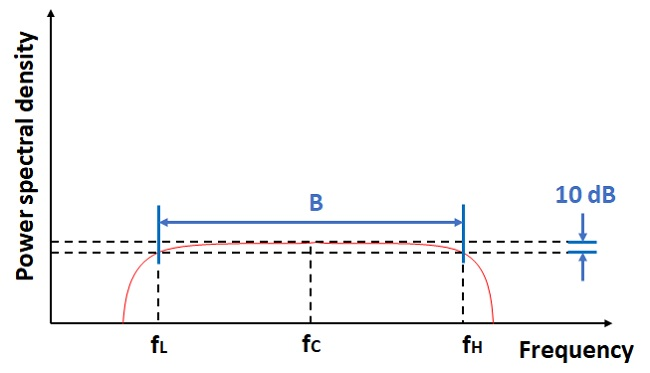
\includegraphics[width=\linewidth]{graphics/UWB_spectrum.jpg}
\caption{Power Spectral Density: Bandwidth B, lower-frequency f\textsubscript{L}, upper-frequency f\textsubscript{H}, \cite{hsu_2021}}
\label{f:UWB_spectrum}
\end{figure}


\subsubsection{UWB supported Nodes}

The IEEE 802.15.4 standard distinquishes between two types of devices.
Full-function device (FFD) are capable of connecting to multiple other devices, receive, transmit and coordinate. Reduced-function device (RFD) on the other hand can only connect to one other device and act as worker. 
In Topological terms RFDs can only operate as leaves, while FFDs can be any node in a network, including leaves.
RFDs therefore are strictly worse, but make up for it by requiering fewer resources, such as memory and power.
When FFDs work as PAN coordinators, they can use short adresses to address any node.
The PAN also has a PAN identifier, to help communication accross multiple networks, while still using the short address.
Each device also has a extended address, that is not assigned by any coordinator, that serves as a universal unique identifier (UUID).


\subsection{UWB MAC}
\label{sec:UWB MAC}

The Mac Layer is part of the Data link layer.
The Mac Frame is the payload of the PHY frame. It carries information about the type of frame, frame-format, security mechanism, adressing and frame validation.
The Mac Layer additionaly provides rules for beacon managment, chanel access.

\begin{figure}[ht!]
	\centering
	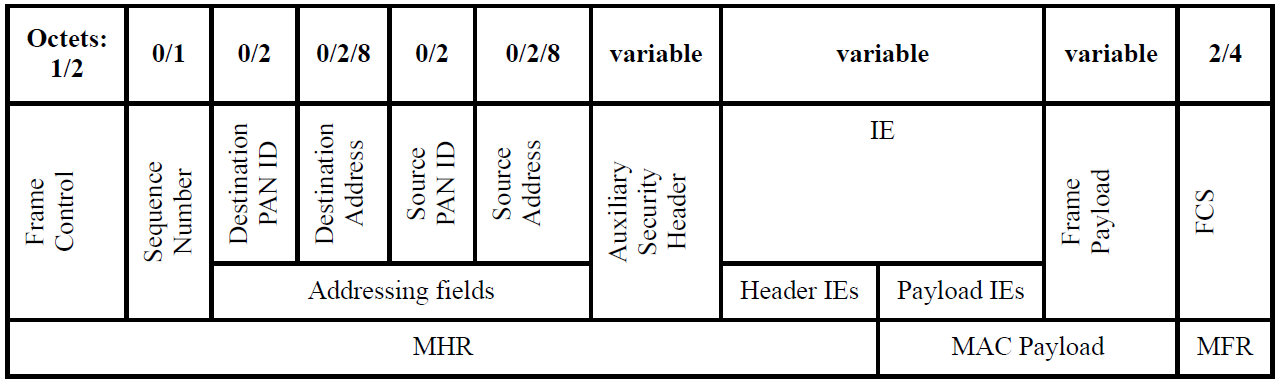
\includegraphics[width=\linewidth]{graphics/general_MAC_Frame_Format.png}
	\caption{General MAC Frame Format \cite{IEEE4-2020-7}}
	\label{f:MAC Frame Format}
\end{figure}


\subsubsection{MAC Frame Format}

Figure \ref{f:MAC Frame Format} shows the composition of a UWB-MAC frame.

In the MAC header (MHR), the Frame Control Field includes information about:

\begin{itemize}
  \item the frame-type
  \item if the Auxiliary Security Header Field is used and in what capacity
  \item if additional frames will follow
  \item if an acknowledgment message is expected
  \item if the message is between different PAN-Networks.
  \item of what type the receiver is (PAN coordinator, device, PAN-Network)
  \item the used frame-format standard
  \item where to find the source address
\end{itemize}

The Sequence Number counts up, helping to keep track of the order in which frames arive.
The Adressing Fields carry the IDs of sender and recipient for the frame.
The Auxiliary Security Header Field only exists if it was specified in the control Field.
It contains additional information needed for the chosen security methode.

There are two parts to the information element (IE).
The header IE specifies additional information about the frame, for example data formating information or chanel time allocation.
The the payload IE specifies the length and data-type of the payload field.
The payload containes the data that is sent.
It and the IE are of variable length, depending of the frame-type and data-length.

The MAC footer (MFR) marcs the end of the frame.
It only contains the frame checking sequence (FCS), that can be used to detect corrupted frames using cyclic redundancy checks.

\subsection{UWB PHY}

\subsubsection{PHY Chanel}

The IEEE 802.15.4z amendment defines 16 channels for communication for HRP UWB. 
A chanel is defined by its center frequency.
UWB devices can transmit on three different bands, high band, low band and sub-gigahertz.
For each band their is one chanel that is mandatory to support, if a device suports the band.
The other channels are optional, but if two devices want to communicate with each other they need to use the same band.
The bands, 16 chanels and their ranges and which chanels are mandatory can be found in table  (see table \ref{Table:: UWB frequency and channel assignments}).


\begin{table}[ht!]
\centering
\begin{tabular}{|l|l|c|c|}
\hline
\textbf{Channel number} & \textbf{Center frequency (MHz)} & \textbf{HRP UWB band}       & \textbf{Mandatory}  \\ 
\hline
0                       & 499.2                           & sub-gigahertz               &  \checkmark     \\ 
\hline
1                       & 3494.4                          & \multirow{4}{*}{Low band}   &                   \\ 
\cline{1-2}\cline{4-4}
2                       & 3993.6                          &                             &                   \\ 
\cline{1-2}\cline{4-4}
3                       & 4492.8                          &                             & \checkmark      \\ 
\cline{1-2}\cline{4-4}
4                       & 3993.6                          &                             &                   \\ 
\hline
5                       & 6489.6                          & \multirow{11}{*}{High band} &                 \\ 
\cline{1-2}\cline{4-4}
6                       & 6988.8                          &                             &                   \\ 
\cline{1-2}\cline{4-4}
7                       & 6489.6                          &                             &                   \\ 
\cline{1-2}\cline{4-4}
8                       & 7488                            &                             &                   \\ 
\cline{1-2}\cline{4-4}
9                       & 7987.2                          &                             & \checkmark       \\ 
\cline{1-2}\cline{4-4}
10                      & 8486.4                          &                             &                   \\ 
\cline{1-2}\cline{4-4}
11                      & 7987.2                          &                             &                   \\ 
\cline{1-2}\cline{4-4}
12                      & 8985.6                          &                             &                   \\ 
\cline{1-2}\cline{4-4}
13                      & 9484.8                          &                             &                   \\ 
\cline{1-2}\cline{4-4}
14                      & 9984                            &                             &                   \\ 
\cline{1-2}\cline{4-4}
15                      & 9484.8                          &                             &                 \\
\hline
\end{tabular}
\caption{ HRP UWB Frequency and Channel Assignments  \cite{IEEE4-2020-7, IEEE4z}}
\label{Table:: UWB frequency and channel assignments}
\end{table}

\subsubsection{Scrambled timestamp sequence}

The 4z amendment added the option to include a scrambled timestamp sequence (STS) into the frame.
The STS is a cyphered sequence that includes the timestamp and is used for ranging.
It is ment to increase the accuracy and integrtity of the raging results.
Before transmition receiver and sender exchange a randomly generated key.
The key is then used to encrypt the timestamp using the advanced encryption standard (AES) with 128 bits.
This ensured that the signal has not been intersepted and changed, to manipulate the ranging result.
Devices that support STS are called HRP-enhanced ranging capable
devices (HRP-ERDEV).

\subsubsection{Pulse Repetition Frequency}
\label{sec:pule repetition frequency}
The pulse repetition frequency (PRF) is the frequency at wich bursts are sent by the transmitter.
The mean PRF is the average PRF while sending the payload (power switching service data unit PSDU). %https://www.keysight.com/blogs/en/tech/rfmw/2021/07/28/an-overview-of-the-ieee-802154-hrp-uwb-standard
The higher the mean PRF, the shorter the airtime of each frame and allows for faster communication.
HRP-ERDEV use a different mean PRF than general devices.
They can work in Base pulse repetition frequency (BPRF) operating at mean PRF 64 MHz or in higher pulse repetition frequency (HPRF) mode operating above BPRF (Table \ref{f:mean PRF}).

\begin{table}[ht!]
\centering
\begin{tabular}{|l|l|l|} 
\hline
\textbf{Standard}          & \textbf{HRP UWB mode} & \textbf{mean PRF}            \\ 
\hline
802.15.4                   & Non HRP ERDEV         & 3.9 MHz, 15.6 MHz, 62.4 MHz  \\ 
\hline
\multirow{2}{*}{802.15.4z} & HRP-ERDEV BPRF        & 62.4 MHz                     \\ 
\cline{2-3}
                           & HRP-ERDEV HPRF        & 124.8 MHz, 249.6 MHz         \\
\hline
\end{tabular}
\caption{HRP UWB Mean PRF (Based on IEEE 802.15.4 and IEEE 802.15.4z, \cite{IEEE4-2020-7, IEEE4z})}
\label{f:mean PRF}
\end{table} %cite euse eigeni bricht

\subsubsection{Symbol Encoding}
UWB sends symbols by transmitting a burst of pulses that encode the symbol.
Since the pulses have clean edges, the arival time can be measured precisly.
This leads to the burst having two ways to carry information( \cite{QorvoGettingBacktoBasics}):
\begin{itemize}
  \item Binary phase-shift keying (BPSK: Encoding zeros and ones shifting the pulses phases so the burst beak for one has an oposite amplitude to the other. 
Figure \ref{f:UWB_signal_description} shows the singal 101 binary phase-shift keyed. 
Each bit is set twice, to detect problems with transmission.
  \item Burst position modulation (BPM): Changing the timing of the burst so it falls into a different time-slot inside of the possible burst position.	
Figure \ref{f:symbol structure} shows how the burst can be placed in a BPM-interval. 
The burst can't be placed in the guard interval. 
The guard exists to minimize inter-symbol interference from the
signals taking multiple paths.
\end{itemize}

\begin{figure}[ht!]
	\centering
	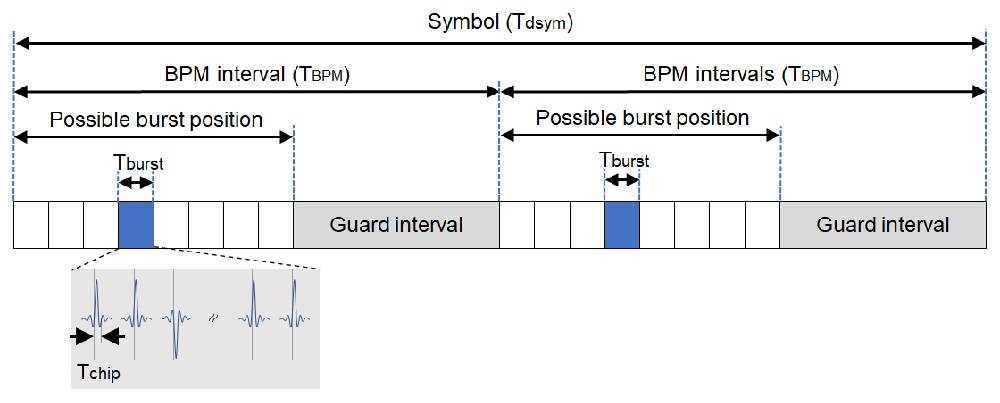
\includegraphics[width=\linewidth]{graphics/HRP_UWB_PHY_symbol_structure.jpg}
	\caption{HRP UWB PHY Symbol Structure \cite{hsu_2021}}
	\label{f:symbol structure}
\end{figure}

One or both of these encoding-strategies can be used in a uwb transmission.
The poition of the pulses inside of the burst (see figure \ref{f:UWB_signal_description})  relative to each other can be used to detect the presence of multipath effects and adjust for them. 
Using this, precises arrival times for the whole signal can be calculated.

\begin{figure}[ht!]
	\centering
	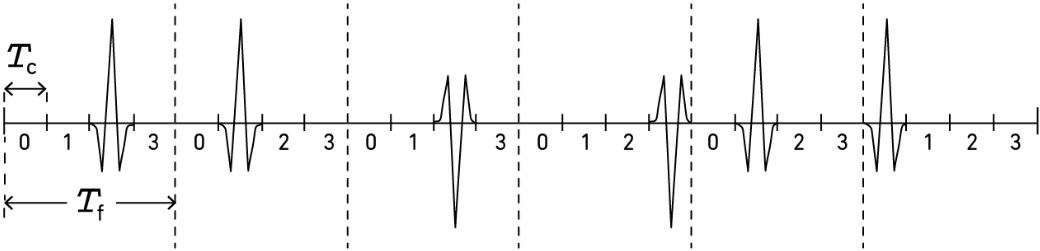
\includegraphics[width=\linewidth]{graphics/uwb_signal_tramsmission.png}
	\caption{UWB signal transmission byte encoding, \cite{QorvoGettingBacktoBasics}}
	\label{f:UWB_signal_description}
\end{figure}

Non-HRP ERDEV use BPM and BPSK.
Some HRP-ERDEV can use only BPSK, using a higher PRF and therefore reducing airtime.








\subsubsection{PHY Frame}
Figure \ref{f:PPDU general} shows a schematic view of a PHY frame as defined by the IEEE 802.15.4 standard.
The Synchronziation header (SHR) containes the information needed to detect the signal and ajust to its parameters.
The PHY header contains meta information about the payload and its encoding.
The PHY payload contains the data that is to be send, namly the MAC frame.

\begin{figure}[!ht]
\centering
\includegraphics[width=\linewidth]{graphics/Schematic_view_PPDU.png}
\caption{Schematic view of a PHY frame defined by IEEE 802.15.4 \cite{IEEE4-2020-7}}
\label{f:PPDU general}
\end{figure}


Figure \ref{f:SHR field} shows the synchronization header, consiting of two parts.
The SYNC section is detectable by the receiver and informs it that a transmission has started.
Depending on the predefined mode, pulses of different length.
The sequence of pulses specify a set of chanels that can be used for communication.
The preamble can also be used to identify a PAN coordinator.

The SHR ends with the Start of Frame Delimiter (SFD).
It indicates that the synchronization has ended and the comming signals will be data, starting with the PHY header. 
It also contains a timestamp which can be used for ranging using time difference of arrival (ToA), see section \ref{TODO: put in this section}


\begin{figure}[!ht]
\centering
\includegraphics[width=\linewidth]{graphics/SHR_field_structure.png}
\caption{SHR Field Structure \cite{IEEE4-2020-7}}
\label{f:SHR field}
\end{figure}	

The PhY header contains all information needed to read the PHY payload (see Figure \ref{f:PHR general}).
The first bit defines the data rate that will be used during the playload transfer (see section \ref{sec:pule repetition frequency}).
The next seven bits define the length of the frame, with a frame length of maximal 128 bytes.
the 10th bit shows if ranging will be used with this frame.
The next bit is reserved.
Bits 11 and 12 define the preamble duration. It specifies how many repetitions are used, which can range from 16 to 4096.
The last 6 bits are single error correct, double error detect (SECDED) bits that form a Hammock block and can be used to correct single bit errors and detecting, but not fixing, double bit errors.

The last part of the PHY frame is the The PHY payload (PSDU).
This contains the the MAC frame, as defined in section \ref{sec:UWB MAC}.

\begin{figure}[ht!]
\centering
\includegraphics[width=\linewidth]{graphics/PHR_field_format_4.png}
\caption{General PHR Field Format \cite{IEEE4-2020-7}}
\label{f:PHR general}
\end{figure}

The 802.15.4z amendment contains optional changes to the PHY frame format if the participaiting devices are HRP-ERDEV devices.
Figure \ref{f:HRP-erdev frame} shows the newly allowed structures for a UWB frame.
Configuration 1 is equivalent to the already existing PHY frame.
The others additionaly contain a scrambled time stamp.
This can be placed in different places after the SHR.
Since UWB can also be used only for ranging without transmitting a message, configuration 3 only contains the SHR and STS, without a payload.

\begin{figure}[ht!]
\centering
\includegraphics[width=\linewidth]{graphics/HRP_ERDEV_frame_structures.jpg}
\caption{HRP-ERDEV Frame Structures \cite{hsu_2021}}
\label{f:HRP-erdev frame}
\end{figure}

Additionally the PHR can be formatted differently (see gigure \ref{f:PHR 4z}. 
The reserved field and preamble duration is removed to make more space for the frame length. This allows to send more data in one frame, increasing the throughput of the UWB communication.

\begin{figure}[ht!]
\centering
\includegraphics[width=\linewidth]{graphics/HRP_ERDEV_HPRF_mode_PHR.png}
\caption{PHR Field Format for HRP-ERDEV in HPRF Mode \cite{IEEE4z}}
\label{f:PHR 4z}
\end{figure}


\subsection{Two-way ranging}
\label{ss:two_way_ranging}
The IEEE 802.15.4z UWB standard describes two ranging methods, single-sided two-way ranging (SS-TWR) and Double-sided two-way ranging (DS-TWR).
In both instances, the distance measurement is done by calculating the time of flight (ToF) of a signal sent between two device using timestamps and multiplying it with the speed of light. 
In this section both SS-TWR and DS-TWR will be discussed.
In all other parts of the thesis,two-way ranging(TWR) refers to DS-TWR.




\section{Related Work} % application of concepts


\subsection{Artwork Tracking}


Since art preservation is an old field and temperature, humidity, light and vibrations have been known to be detrimental to most artworks, especialy paintings, most research in this direction is older than 20 years \cite{mecklenburg1991mechanical, michalski1991paintings, saunders2004effect}.
Still, the envention of new technologies, such as pattern recognizion using artificial inteligence, improvement on existing tools like infrared imaging and a active need for solutions have kept the resaech into artwork preservation an active field \cite{borg2020application, schito2017integrated}.
One such new technologies are sensor networks, which have become widespread in the field of art-preservation \cite{shah2016customized}.


Artwork tracking during transportation has not been a major focus in academia.
The most relevant related research was done by Fort et al. \cite{landi2022iot}.
They developed a low-cost, low powered sensor node to track temperature, humdity, pressure and vibrations of artwork and wooden structures.
The sensor node would then report its findings to a remote server.
They confirmed the validity of their sensor in a series of experiments, that were performed in a static building.
They also presented a theoretical framework for their sensor to be used in a transportation scenario, but they do not report having implemented or tesed this system.
Their sensor used an ascelerometer to detect vibrations, and the Bosch BME280 sensor to detect pressure, temperature and humidity.
Their sensors did not build a network and were not queried, but reported their findings directly to either a wlan router or a ble-capable smart-device.
The research of Fort et al. showed the value of low-cost sensors in the detection of threats to artwork.

\subsection{Sensor Networks}

Wireless Sensor Networks (WSN) have become a central aspect if IoT.
Researchers have tried to focus on the most prevelant problems arrising from the development of NSWs, mainly power managment, security and privacy, data integrity and avaliability \cite{gulati2022review}.


\cite{garg2021healthcare} researched WSNs outside of the controlled environment of a house. They propose a WSN that can track thevitals of mountainiers and call for help when measurements have dangerous values. 
They used an Ardruino Mega board equiped with a radio transiever, using LoRa with a star-topology, was used.


\cite{jones2021wireless} created a WSN of NRF24101 board that is intended to monitor linear infrastructures like deepsee wires, using radio and wifi for communication. Using deep sleep they were able to optimize energy usage so the sensor is predicted to last five years on batery.


\cite{spandonidis2022evaluation} used an acelerometer to detect vibrations in pipeline to discover leaks. 
They used a narrowband connection for communication and GPS for localization.
Their sensors could query each other for data, to provide a more complete image of the situation.


\subsection{Wireless ranging}

\cite{li2024indoor} made an overview of publications envolving positioning systems for industrial settings. 
They looked at the positioning systems in papers using RFID, BLE, UWB, Wi-Fi and ZigBee. They found that UWB consistently reported the highest accuracy of these methods.
UWB was the least affected by multipath-effects, although it was still the most common issue with this technology.


Early research of ranging using UWB was done by Gezici et al. \cite{gezici2008survey, gezici2005localization}.
These papers gave an overview of the different positioning systems for UWB, angle of arival, recived signal strength, time of arrival and time difference of arival.
Time of arival and time difference of arrival were studied further in these publications, presenting errorsources and mitigation tools.


Early research focused on augmentation of UWB ranging methods.
\cite{venkatesh2007nlos} proposed using integer programs for midigating the error for ranging without line-of-sight.
\cite{guvencc2007nlos} tried to solve the same issue by using methods based on the statistics of multipath-effects.
BiasSub and BiasRed was proposed to reduce the bias in time difference of arival, by appling of a well-known algebraic explicit solution for source localization  \cite{ho2012bias}.
\cite{fan2017performance} emproved uwb ranging by eliminating random error. They did this by pre-filtering, using a anti-magnetic ring to eliminate outliers and using the double-state adaptive Kalman filter to improve position accuracy.
Newer research has also begone incorporating neural networks into UWB positioning systems \cite{stahlke2020nlos, ridolfi2021uwb, che2020machine}.

UWB localization has been used in many applied context.
It has been proposed for pedestrian tracking \cite{otim2019effects}, drone flying \cite{macoir2019uwb},robot navigation \cite{zhu2020adapted}, navigation system for visualy impared people \cite{rosiak2024effectiveness} and tracking people in buildings \cite{elbaum2024investigating}.
UWB positioning systems are particularly interesting for industrial IoT settings.
\cite{barbieri2021uwb} measured the performance of three different UWB antennas, Qorvo, Sewio, and Ubisense. They measured a lot of multiplath-effects in such a complex environment. The midigated this by employing a Bayesian filtering method.
\cite{belli2024cloud} used UWB positioning in combination with Real-time kinematic positioning, to track workers while monitoring the factory. The goal was to trigger an alarm if a dangerous situation occured.

%\chapter{Design}

This section presents the principle design of the monitoring system.
In the section \ref{ss:hardware} the components used are presented.
Section \ref{Dataflow} desctibes the functionalities and responsibilities of the system components.
In Section \ref{ss:network} the network topology and data-flow is discueed

\section{Hardware}
\label{ss:hardware}

This sectiondescribes the hardware used in the project. The setup consists of two distinct components: the artwork-tags, of which there are four, and one Phone that provides the interface to the user. The tag itself consists of 4 components:
\begin{enumerate}
	\item nRF52840 Microcontroler
	\item DWM3000 UWB Shield
	\item DHT22 temperature and humidity sensor
	\item MPU6050 accelerometer and gyroscope
\end{enumerate}

\subsection{Microcontroler}
The fundament of the artwork-tag is build by the nRF52840 DK microcontroller developed by Nordic Semiconductors. 
It is part of the nRF52 series of microcontrollers intended for development.
The nRF52840 DF is specialiezed for ble communication, for which it already includes the neccesary components.
It is compatible with the nRF52 Software Development Kit (SDK), also developed by Nordic Semiconductors.
The SDK makes it possible to use the ble functionalaties and to control the pins. It aslo includes implementations for a plethera of pin based protocols.
It contains 58 pins, 48 of which are data-pins and manage the power suply for additional modules, which includes 3.5 and 5 Volt supply pins.
32 of the pins are installed in the same way as the pins on the Ardruino uno, making it compatible with many peripherals that were designed with this common board in mind, such as the dwm3000.
The remaining ten pins are enough to attach the sensors to.
The nRF52840 DK includes a USB-B port that is used for Powersuply. Additionally it is connected to two pins and is used for UART-communication and for debugging.
The nRF52 was chosen since it was avaliable and previous projects have been done with it in compination with the DWM3000 shield.
As a result a lot of initial setup was already avaliable.

\subsection{UWB shield}
For communication between the tags as well as distance measurement the DWM3000 UWB-shield developed by Qorvo was chosen.
The DWM3000 is a commonly used device for research involving UWB \cite{coppens2022overview, leu2022ghost, stocker2022performance}.
It allows low level access, but includes an SDK written in C that makes a lot of the processes transparent to the user, if they wish.
The SDK uses the Serial Peripheral Interface (SPI) for communication between the shield and the microcontroler.



\subsection{Humidity and temperature sensor}

For humidity and temperature sensors I decided to use the DHT22(AM2302) produced by Guangzhou Aosong Electronic Co. \cite{AM2302}. 
It is a comonly used sensor in IoT monitoring systems \cite{ahmad2021evaluation}. 
The vendor claims a temperature range from -40\degree to 80\degree Celsius with a precision of 0.5\degree. 
\cite{ahmad2021evaluation} could experimentaly confirm that errors did not exceed 0.1\degree Celsius. 
They also concluded that the sensor is slow in detecting temperature change. 
This is also confrimed by the user manual \cite{AM2302}, that states a read-interval of less than 2s is not possible. 

The humidity sensor can detect the full range from 0\% to 99.9\% humidity, with an advertised maximum error of 2 percent-points \cite{AM2302}.
I could not find any research that confirmed or denied these claims.

The DHT22 sensor uses three pins from the microcontroler, two pins for power suply and ground and one for single-bus communication.
Since no SDK for this type of communication has been build for the nRF52 board series, it had to be implemented manually by reading the high and low voltage on the communication pin and, detecting headers and footers and parsing the binary messages. 
Dmitry Sysoletin published a project on github (\url{https://github.com/DSysoletin/nRF52_DHT11_example}) that handles the communication between an nRF52840 and a DHT11 sensor. 
Since the communications is mostly the same, I used his implementation, but changed the parsing of the actual data to fit the encoding used by the DHT22.

\subsection{Accelerometer and Gyroscope}
The MPU6050 sensor produced by InvenSense Incorporated provides accelerometer and gyroscope data.
The accelerometer reports the acceleration in the three cardinal directions in meters per second.
The Gyroscope reports the rotation around the threee euclidean axis in degrees per second.
In this project the accelermoterdata was not used, just the gyroscope.

The MPU6050 uses 4 pins, two for power suply and ground and two communication.
The Sensor communicates using the I2C protocoll, a serial synchronus communication system.
The microcontroller acts as the master and would in theory suport multiple workers on the same bus. 
Here only the MPU6050 uses I2C and is therefore the only worker.
While the nRF52 SDK does not supply a I2C API, it offers a Two Wire Interface (TWI) implementation that is compatible with the I2C protocoll.
It even used to offer MPU6050 specific support in the older SDK. 
I was able to port this older code to the current SDK.

\subsection{Tag technical plan}
The microcontroler builds the base of the Artwork-Tag. 
The other devices are attached to it over the avaliable pins.
In the nRF52 SDK each data pin is assigned an integer value. 
These often correspon with the name of the pin according to the nRF52830 DK manual, but not always.
I will use the names given in the manual to describe the pins.
Pins are the methods by which a microcontroller controls its peripheras.

Some pins are intended for power supply.
On the NRF52840 these pins are located in section P1, see table \ref{table:ArdruinoPins}.
The three VDD pins suply electricity with a Voltage of 3.5 Volts.
A secondary power supply that uses 5 Volts is also avaliable.
What voltage is needed depends on the periipheral.
In this case, the DHT22 runs on 3.5 Volts, while the MPU6050 is made for 5 Volts.
The P1 section also contains two ground pins, that need to be connected to the peripherals and a reset pin, so restart the microcontroler.
The last pin is not connected (N.C.).
There are additional ground pins in sections P4 and P24 of the board.

The other pins are called data pins.
By using voltage modulation these pins can transfer data and therefore be used for communication.
The nRF52840 has a I/O voltage of 3.3 Volt.
This means that a voltage of 3.3 Volt corresponds to a \textit{Logic high} and 0 Volts represents a \textit{Logic low}.
This allows the data pin to transfer communication in a binary encoding.
How a signal is interpreted is defined by the used communication protocol.
The MPU6050 for example uses the I2C protocol and uses 2 datapins.
This defines that one pin is used for a serial clock and the other pin transmits data.
For the data transmission the protocol defines what a package looks like.
This includes the start condition, the voltage characteristics that signal the beginning of a package, adressing, data encoding, acknowledgments and stop condition.

The DHT22 sensor does not use a given communication-protocol.
It uses one data-pin to report its sensor data.
How that data is encoded to high and low voltage is specified in the user manual \cite{AM2302} and has to implemented manualy.

The DWM3000 shield is mounted on the 32 pins ment for arduino one connections. 
All pins are forwarded and can be used by other devices, in a common ardruino-stackable style.
If they are data-pins they will share the data.
Table \ref{table:ArdruinoPins} shows which devices use which pins.
The only pin shared by multiple devices are power and ground pins.
The microcontroler suplies enough power to support this.

The sensors are attached to the same powersource and ground as the shield, but use different data-pins.
The DWM3000 leaves enough pins unused that both sensors could be attached to them.
Since it is not visible which pins the shield leaves free, I decided to use data-pins that are not attached to the DWM3000 in any way.
Table \ref{table:otherPins} shows how the sensors are connected to the remaining open pins.

\begin{table}[]
	\centering
	\begin{tabular}{l|l|l|l|l|}
		& Pin & \rotatebox{90}{DWM3000\phantom{.}} & \rotatebox{90}{DHT22}  & \rotatebox{90}{MPU6050\phantom{.}}   \\
		\hline \multicolumn{1}{|l|}{\multirow{10}{*}{\rotatebox{90}{P4}}}
		& P1.10  & \checkmark    &             &             \\
		\multicolumn{1}{|l|}{} & P1.11  & \checkmark    &             &             \\
		\multicolumn{1}{|l|}{} & P1.12  & \checkmark    &             &             \\
		\multicolumn{1}{|l|}{} & P1.13  & \checkmark    &             &             \\
		\multicolumn{1}{|l|}{} & P1.14  & \checkmark    &             &             \\
		\multicolumn{1}{|l|}{} & P1.15  & \checkmark    &             &             \\
		\multicolumn{1}{|l|}{} & GND    & \checkmark    &             &             \\
		\multicolumn{1}{|l|}{} & P0.02  &               &             &             \\
		\multicolumn{1}{|l|}{} & P0.26  & \checkmark    &             &             \\
		\multicolumn{1}{|l|}{} & P0.27  &               &             &             \\
		\hline \multicolumn{1}{|l|}{\multirow{8}{*}{\rotatebox{90}{P3}}}
		& P1.01  & \checkmark    &             &             \\
		\multicolumn{1}{|l|}{} & P1.02  & \checkmark    &             &             \\
		\multicolumn{1}{|l|}{} & P1.03  & \checkmark    &             &             \\
		\multicolumn{1}{|l|}{} & P1.04  & \checkmark    &             &             \\
		\multicolumn{1}{|l|}{} & P1.05  & \checkmark    &             &             \\
		\multicolumn{1}{|l|}{} & P1.06  & \checkmark    &             &             \\
		\multicolumn{1}{|l|}{} & P1.07  & \checkmark    &             &             \\
		\multicolumn{1}{|l|}{} & P1.08  & \checkmark    &             &             \\
		\multicolumn{1}{|l|}{} & P1.10  & \checkmark    &             &             \\
		\hline \multicolumn{1}{|l|}{\multirow{8}{*}{\rotatebox{90}{P1}}}
		& VDD    &               &             &             \\
		\multicolumn{1}{|l|}{} & VDD    &               &             &             \\
		\multicolumn{1}{|l|}{} & RESET  &               &             &             \\
		\multicolumn{1}{|l|}{} & VDD    & \checkmark    & \checkmark  &             \\
		\multicolumn{1}{|l|}{} & 5V     & \checkmark    &             & \checkmark  \\
		\multicolumn{1}{|l|}{} & GND    & \checkmark    & \checkmark  & \checkmark  \\
		\multicolumn{1}{|l|}{} & GND    & \checkmark    &             &             \\
		\multicolumn{1}{|l|}{} & N.C.   &               &             &             \\
		\hline \multicolumn{1}{|l|}{\multirow{6}{*}{\rotatebox{90}{P2}}}
		& P0.03  & \checkmark    &             &             \\
		\multicolumn{1}{|l|}{} & P0.04  & \checkmark    &             &             \\
		\multicolumn{1}{|l|}{} & P0.28  &               &             &             \\
		\multicolumn{1}{|l|}{} & P0.29  &               &             &             \\
		\multicolumn{1}{|l|}{} & P0.30  &               &             &             \\
		\multicolumn{1}{|l|}{} & P0.31  &               &             &             \\
		\hline 
	\end{tabular}
\caption{Adruino compatible pin assignment}
\label{table:ArdruinoPins}
\end{table}

\begin{table}[]
	\centering
	\begin{tabular}{l|l|l|l|l|}
		& Pin & \rotatebox{90}{DWM3000\phantom{.}} & \rotatebox{90}{DHT22}  & \rotatebox{90}{MPU6050\phantom{.}}   \\
		\hline \multicolumn{1}{|l|}{\multirow{8}{*}{\rotatebox{90}{P6}}} 
		& P0.00  &               &             &             \\
		\multicolumn{1}{|l|}{} & P0.01  &               &             &             \\
		\multicolumn{1}{|l|}{} & P0.05  &               &             &             \\
		\multicolumn{1}{|l|}{} & P0.06  &               &             &             \\
		\multicolumn{1}{|l|}{} & P0.07  &               &             &             \\
		\multicolumn{1}{|l|}{} & P0.08  &               &             &             \\
		\multicolumn{1}{|l|}{} & P0.09  &               &             &             \\
		\multicolumn{1}{|l|}{} & P0.10  &               &             &             \\
		\hline \multicolumn{1}{|l|}{\multirow{18}{*}{\rotatebox{90}{P24}}} 
		& P0.11  &               &             & \checkmark  \\
		\multicolumn{1}{|l|}{} & P0.12  &               &             & \checkmark  \\
		\multicolumn{1}{|l|}{} & P0.13  &               & \checkmark  &             \\
		\multicolumn{1}{|l|}{} & P0.14  &               &             &             \\
		\multicolumn{1}{|l|}{} & P0.15  &               &             &             \\
		\multicolumn{1}{|l|}{} & P0.16  &               &             &             \\
		\multicolumn{1}{|l|}{} & P0.17  &               &             &             \\
		\multicolumn{1}{|l|}{} & P0.18  &               &             &             \\
		\multicolumn{1}{|l|}{} & P0.19  &               &             &             \\
		\multicolumn{1}{|l|}{} & P0.20  &               &             &             \\
		\multicolumn{1}{|l|}{} & P0.21  &               &             &             \\
		\multicolumn{1}{|l|}{} & P0.22  &               &             &             \\
		\multicolumn{1}{|l|}{} & P0.23  &               &             &             \\
		\multicolumn{1}{|l|}{} & P0.24  &               &             &             \\
		\multicolumn{1}{|l|}{} & P0.25  &               &             &             \\
		\multicolumn{1}{|l|}{} & P1.00  &               &             &             \\
		\multicolumn{1}{|l|}{} & P1.09  &               &             &             \\
		\multicolumn{1}{|l|}{} & GND    &               &             &             \\
		\hline
	\end{tabular}
\caption{Non-Adruino compatible pin assignment}
\label{table:otherPins}
\end{table}


\section{Architecture}
\label{ss:dataflow}

In order to discuss how the dataflow works, first the section \ref{ss:responsibility} will establish what services are implemented in each part of the system.
The section \ref{ss:dataflow} will explain what triggers events and how they are handled inside the system.

\subsection{Responsibilities}
\label{ss:responsibility}
The system consists of the tags, the sensor network and the phone.
These parts all have their own responsibilities.

\textbf{Tag:} 
The tag is responsible to manage its sensors. 
It has to do correct setup and converts its output into a understanable form.
The tag can performe ranging with all its neighbours.
Additionaly the tags are responsible to search for networks to join, and react aprobiatly to network request, be those queries for sensor data, ranging requests or network managment jobs. 
The tags provide a unique, secure universal identifier, to be used by queries or the network.
How this is done is part of the certify project and will not be discussed in this thesis.
The tag is also responsible for its own power managment.
This is not the focus of this thesis and will only be mentioned when relevant.
A guideline on powermanagment will not be provided here.

\textbf{Network:} The network is responsible to keep track of all tags taking part in the network. 
It offers a joining protocol for new devices and remains stable when devices leave or become unavaliable. 
It offers the possibility for phones to connect to the network. 
It ensures quieries from phones get transported to the correct tag and the answers to the correct phone.
It ensures a network topology that corresponds to a graph that is at least 3-connected.
On request it returns a list of connected devices to the phone.

\textbf{Phone:} The phone connects to the network via the provided method.
It offers a graphical user interface (GUI) to be used by the driver.
The GUI offers a method for the driver to set the acceptable ranges for all sensor data.
Additionaly it offers a method to set query intervals-length.
The phone is responsible to query sensor data for each tag and masurement once in each interval.
The phone has to evaluate the answer.
The phone has to report the results to the driver using the GUI.
If a parameter falls outside of the acceptable range for its type, the phone is responsible to alert the driver to this fact.

The certify project also plannes to collect the sensor data on remote servers using a 4G connection.
The plan is to equip each tag with antennas to allow it to send the data directly to the server itself.
Since this is not a part of this thesis, the responsibility for the tag to do this was not added to a list.
A known problem with this plan is, that a 4G connection is not always possible.
Since small tags have very limited memory, the plan to store the sensor data on the tag is not pheasible.
If the setup presented in this thesis is used, it would allow for the storage of the data on the phone, which has a much larger memory.
This again was not added, since it is not part of this thesis.

\subsection{Dataflow}
\label{ss:dataflow}

\begin{figure}[ht!]
	\includegraphics[width=\linewidth]{graphics/schematics/obervation_loop.png}
	\caption{Sequence diagram of setup and oberservation loop. Setup is performed once, oberservation loop repeats until stopped.}
	\label{f:observation_loop}
\end{figure}

How a tag connects to the network is described in the section \ref{s:network}.
Figure \ref{f:observation_loop} shows a sequece diagram ob the setup and main observation loop of the system.
On the top the communicating parts are listed.
\begin{itemize}
	\item Human is the driver of the truck
	\item Phone is the phone used by the Human
	\item Network consists of all the tags that are used and the network they build.
	\item Connected Tag is part of this network, but is listed seperatly. It represents the tag that is communicating to the phone
	\item Tag j is also part of the Netowrk. It represents the tag that is queried during the observation loop
\end{itemize}
Phone and Human communicate by using a GUI. Phone and Connected Tag commuincate using BLE. Every communication inside the network happens using UWB. This includes the communication between the Connected Tag, the network and Tag j. \\
When the phone wants to connect to the network, it looks for advertised BLE devices.
It then displays the devices to the user and lets him pick one.
The phone then pairs to the chosen tag, making it the connected tag and the phones connection to the network of tags.
Once connected to the network, the phone will promt the human to enter the parameters.
These consist of:
\begin{itemize}
	\item Upper and lower limit for sensor data, like temperature and humidity
	\item Maximal displacement value for distance and gyro. These values represent the maximal difference in registered values that is allowed for positional measurements.
	\item Time between measurements. This gives the time period that will pass between measurements for each device and measurement type.
\end{itemize}
Once the parameters chosen, the user can start the observation.\\
Each iteration of the observation loop begins with a call to the network for a list of all tags currently in the network.
Since the tag network is a dynamic sensor network, the tags in the network can theoretically change. 
In practice this should onyl happen, when artwork is unloaded or if a tag becomes faulty.
The request for the list is transmitted to the connected tag ober BLE, which than queries the network for all conected devices.
The responde is returned to the Phone.
The phone then starts a nested loop, iterating over the list of tags and the list of metrics caputred by the system.
For each measurement and tag combination (i,j) the phone contacts the connected tag for the value, which in turn queries the network.
Once the message has arrived at the tag j, tag j gets measurement i. In case of sensors this intails contacting the sensor and requesting a value.
If metric i is a distance measurement, tag j will commence a two-way ranging operation over UWB with all its registered neighbours and will report the list of distances, together with the tag-adresses they correspond to.
Metric i is then transported over the network back to the connected tag and finaly to the phone.
The phone must then evaluate the retrieved data. \\
During the evaluation process, the phone creates an evaluated measurement, and marks it as problematic or unproblematic.
What the evaluation looks like depends on the metric.
\begin{itemize}
	\item For most metrics, like humidity and temperature, the evaluated measurement is equivalent to the received measurement. It is then checked, if the measurement falls into the aceptable measurement parameters, set by the human.
	If it does not, the evaluated value is marked as problematic.
	\item Some metrics require comparisment to the previous data. The gyroscope reports the current orientation of the tag.
	This is then compared to all previous measurements and the maximal angular difference forms the evaluated measurement.
	If the evaluated metric is bigger then allowed by the set parameters, the measurement is marked as problematic
	After evaluation the original measurement is added to the list of previous measurements.
	\item The distance measurement has a unique evaluation process, which is describbed in section \ref{ss:distance_eval}.
\end{itemize}
Once the data evaluation is done, the evaluated measurement is presented to the user over the GUI, together with the adress of the tag it belongs to.
If the evaluated measurement is problematic, the driver it alarmed.


\subsubsection{Distance evaluation}
\label{ss:distance_eval}
The goal of the distance evaluation is to build a working model of where every tag is.
To achieve this, a quadratic program is solved, to get the coordinates of all tags.
The steps to do this are as follows:
\begin{enumerate}
	\item Get a list of all current tags, $T:=\{ t_1, t_2, ... \}$.
	\item For each tag, get the last known distance measurements and put it into a set $S_D:=\{ (t_i, t_j, d_{ij}) \} $, where $t_i$ is the tag which measured, $t_2$ the tag that was measured to and $d_{ij}$ the distance measured.
	\item If a tag has no distance measurements, remove it from the list.
	\item Assign each tag $t_i$ a position in a 3D coordinate system, $(x_i,y_i,z_i)$
	\item Pick one random tag $t_{o}$.
	\item Set the values $x_{o},y_{o},z_{o}$ all to 0.
	\item Create the objective function: $L(X,Y,Z) = \sum\limits_{t_i, t_j, d_{ij} \in S_D}|(x_i-x_j)^2+(y_i-y_j)^2+(z_i-z_j)^2-d_{ij}^2|$. For x,y and z use variables for all but the six values set in step (6).
	\item Solve the quadratic program consting of the Objective function L and no constrains.
\end{enumerate}
Quadratic Programs in general are NP-Hard, but Quadratic Programs with a convex function can be solved efficiently.
$(a-b)^2$ and $c$ are convex functions.
The sum uf a convex function is always a convex function.
The objective function in (7) only sums up convex functions and is therefore convex itself.
The quadratic program can therefore be solved efficiently.\\
By setting the values of tag $t_{o}$ to zero, the results of the quadratc function becomes grounded.
It is not strictily nessecary, but without it the returned solution could have values anywhere in the Euclidean space.
by setting one tag to the coordinates at theo origin, the solution will place the other tags near that region.
There are still an infinte amount of solutions to this quadratic function, since all solutions can be roatated around any axis and still return the same objective function.

\begin{figure}[ht!]
	\begin{subfigure}{.4\linewidth}
		\centering
		\includegraphics[height=150px]{graphics/schematics/connected_dots.png}
		\caption{3-edge connected graph}
	\end{subfigure}
\hspace{1cm}
	\begin{subfigure}{.4\linewidth}
		\centering
		\includegraphics[height=150px]{graphics/schematics/connected_dots_k_connected.png}
		\caption{2 connected graph}
	\end{subfigure}
	\caption{ Left: Five dots, all having at least two connections, still blue can move independently. Right: minimal 2-connected graph, no movement possible. }
	\label{f:connected_dots}
\end{figure}

For a point to be clearly placed in Euclidean space, three distances to other points have to known.
This alone is not sufficient to insure a unique results.
The left of Figure \ref{f:connected_dots} illustrates this point in two-dimensional space.
Every circle is connected to two others, still the blue circles can move without the whole figure moving.
What is needed to keep every point static is for known distances and tags to build a four-connected graph (three in two dimensions).
The left of Figure \ref{f:connected_dots} shows a sollution of the problem on the right by creating a three-connected subgraph.

Once the coordinates for all tags are found, they are compared to previous results.
For each tag the phone calculate by how much it has moved.
The evaluated measurment is the distance of the tag that has moved the most.
If the evaluated measurement is larger then the maximal allowed displacement, the measurement is problematic.



\section{Network}
\label{s:network}

For the presented network to work, tags need to be ranked.
This means that for each tag pair $i,j$, one can either say that $rank(i)<rank(j)$ or $rank(j)<rank(i)$.
To achieve this, the universal unique identifiers are used.
No matter what form the UUID has, it can be converted to an integer, by simply interpreting its binary code as one.
Since the UUIDs are unique, no to tags will have the same resulting integer.
When refering to the rank of a tag in this section, the integer representing the UUID is intended.

The tags inside the truck, while not connected to a phone, form a dicentralized mesh using UWB for communication.
Each tag keeps two list, a list of known devices and a list of neighbours.
When a new tag joins the network, it sends a joining request over UWB, containing its universal unique id (UUID), using a weak signal.
All tags in the network that receive this request add the new device to their list if known devices. 
If the new devices also has a heigher rank, they additionaly add it to their list of neighbours.
They then answer by sending their own UUID and adress back to the new tag.
By waiting an amount of time that correlates with their UUID, the tags in the network can ensure, that their answers don't overlap.
The new tag adds the received adresses and UUIDs to its known device list. If the rank of the added tag is also has a higher rank then the new tag, it will add it to the list of neighbours.
If the new tag now has four neighbours, it stops. Otherwise it will repeat the process with a incresasingly stronger signal, until it has either found four tags with higher rank or reached maximum signal strength.
Afterwards it starts addvertising its BLE connection.
This concludes the network joining process.


A user with a phone can connect to any of the advertised BLE connection.
Once that happens, the tags in the tracks will switch from their dicentralized mesh to a star-topology, with the connected device serving as the coordinator.
The coordinator will inform all tags about its new status, by sending a message using a strong UWB signal.
The tags will then acknowledge this message in order of rank.
The tags in the network will still keep their stored neighbours and known devices.
The coordinator records a list of all acknowledgemtns, thus creating a list of all devices in the network.


The phone can request the list of all tags from the coordinator.
The phone can now also query the tags in the truck by sending the query to the coordinator over BLE, which then will pass it directly to the apropriate tag using BLE.
For all sensor data, this is a simple call and response request. \\
If a distance measurement is queried, the tags takes the following steps:
\begin{itemize}
	\item It conducts a UWB two-way ranging session with each tag in the neighbour list.
	\item It reports those results to the coordinator tag.
	\item It orders all received distances.
	\item It keeps the tags with the four lowest distances and deletes the rest from the neighbour list.
\end{itemize}
The first time a distance is requested, the tag will perform more ranging sessions then necesary to build a 4-connected graph.
Afterwards it only perform ranging with four other tags, unless a new device was added.
If a ranging session does not report a result, because a tag left or became unavaliable, the tag adds ads the tag with the shortest previously measured distance and higher rank from the list of known devices back intro the list of neighbours.


This design mirrors the algorithm proposed by \cite[khan2007simple] and presented in section \ref{ss:k_connected_explained}.
It creates an approximation of a minimaly weighted k-connected subgraph, based on the measured distances.
This is allowed, since the distances are in euclydean space, which when mapped to a graph forms a metric graph.
As discussed in section \label{ss:distance_eval}, a four-connected graph is needed to uniquly identify the position of each tag.
The graph should be minimaly weighted, so that measurements are between tags that are as close as possible to each other.
This reduces the multipath effect and theirfore increases precision.


If the tags are not connected to a phone and report their data to a remote server, they can still use the same distance-measurement, to approximate the k-connected subgraph.
The quadratic program can then be calculated on the server.
%\chapter{Implementation}
\label{c:implementation}

In this section, the implementation that was used for the experiment is discussed.
In section \ref{s:tag} the implementation of the tags is presented.
Section \ref{s:app} shows the implementation of the App.

\section{Tag}
\label{s:tag}
The software of the tags consits of n modules:
\begin{enumerate}
	\item Temperature and humidity sensor
	\item Gyroscope
	\item UWB network
	\item Two way ranging
	\item BLE communication
	\item Job handler
\end{enumerate}
The following subsections will discuss the first five modules, followed by how they interact using the job handler module.
The section \ref{ss:combination} discusses chalanges from combining these modules and how they were solved.

\subsection{Temperature and humidity module}
\label{ss:temp_hum_module}
This module is responsible for managing the DHT22 humidity and temperature sensor.
It is responsible to setup the sensor during initial startup and to provide the sensors measurements when queried.
The DHT22 sensor communicates using only one data pin, pin 13, which will be referd to as the data pin in this section.
Dmitry Sysoletin created an implementation \ref{sysoletin2021nrf52_dht11} for the DHT11 sensor together with the nRF52840 board that build the basis for this implementation, by addapting it to the DHT22 and adding functionalities needed by the job handler module.


Since the DHT22 is a very simple sensor, using single bus comunication, not much setup is needed.
The evaluation of the sensor data requires that the voltage of the pin is read out in pre-defined intervals, when reading the sensor data.
To do this, a clock is required.
This resource has to be reserved an initiated at startup.
This is the only setup that is required for the DHT22 sensor.


To initiate a sensor-read the voltage of the data pin is set to 0.
When the sensor is in standby mode, the data pin is on \textit{logic high}, and when set to \textit{logic low}, the sensor will respond with a read of its current value.
A schematc view of a sensor read of the DHT22 can be seen in Figure \ref{f:dht22_signal}.
The temperature and humidity module will then check the Pin State in intervals of 5ms, until a \textit{logic low} is registered, signalling that the sensor has registered the request. 
The module will now monitor the pin state, waiting for \textit{logic low} followed by a \textit{logic high}, this beeing the start condition of the data transfer. \\
The data is transfered in five chunks of eight bits.
Each bit is preceeded by a prolonged \textit{logic low} state, that is detected by the module
The module then proceeds to write the state of the data pin into a 8-bit buffer, \textit{logic high} corresponding to a 1 and \textit{logic low} to 0.\\
Once all five chunks are read, the communication has ended and the module can verify the data.
The first two bytes correspond are combined to form the temperature information in celcius, the second and third form the humidity.
Both values are multiplied by 100 and stored in a 16-bit integer. This doesn't loose data, since the sensor only measures up to a precision of 1 after the decimal point.
The data beeing stored in an integer help with data transfer.
It will be converted back on the phone.
The fith chunk contains the parity and is used to accept or reject the humidity and temperature values.
If the process fails at any state, -100\degree C is returned for the temperature and -100% for humidity.
These form both impossible values, since humidity can't be negative and the DHT22 sensor can only detect temperatures as low as -20\degree C.


\begin{figure}[ht!]
\centering
\includegraphics[width=\linewidth]{graphics/DHT22_signal.png}
\caption{Signal of a DHT22 sensor-read as presented in the manual \cite{AM2302}.}
\label{f:dht22_signal}
\end{figure}

\subsection{Gyroscope}
\label{ss:gyro_module}
This module manages the MPU6050 gyroscope and accelerometer.
It is responsible to setup the sensor and report its result.
An implementation for the MPU6050 was present in the nRF52 15.3.0 SDK, but is no longer avaliable for the nRF52 17.1.0 SDK, used in this project.
The old implementation was ported to this project.
This consisted of replacing deprecated parts of the SDK with updated ones and adding newly required flags to the build.


MPU6050 sensors use the I2C communication protocol.
The nRF52 SDK does not include an implementation for this protocol, but has a Two Wire Interface (TWI) implementation that is compatible with the I2C protocol.
During startup the TWI module has to be initialized.
This is handled by the SDK, but requires some parameters to be passed.
\begin{itemize}
	\item The Serial Clock Line (SCL) defines what pin will be used for the clock shared in the TWI. This implementation uses pin 11.
	\item The Serial Data Line (SDA) defines which pin is used for the data communication. Pin 12 was used.
	\item The frequency which the TWI uses. It is defined in MPU6050 data sheet, and is 100 kHz \cite{MPU6050}.
	\item The Interrupt priority is a rank that determins, how easyely this process can cause an interrupt. It is set to high.
\end{itemize}
After the TWI service is initiated with these parameters, it is enabled, ensuring that its resources are locked and can not be used by other services.


Afterwards the results from the sensor can be read using the TWI service again.
The TWI-TX requires the adress of the read device and a registry where to write the MPU6050 datasheet \cite{MPU6050}.
The adress of the sensor is the same for all MPU6050 sensors and can be found in the manua
It sets a flag to true once the sensor has writen the data, which then can be read using the TWO-RX function.
The result consist of three 16-bit integers, representing the angular velocity arround the X,Y and Z axis, shown in figure \ref{f:MPU6050_orientation}.\\
Returning this data when queried has only limited use.
It represents a measurement of the current situation.
The caller is more interested what happened since the last query.
Two different implementations for the read of the gyroscope were used during the experimental phase of this thesis.
One would try to return the current orientation of the tag. This read will be called the \textit{orientational read}.
The other would return the maximal registered angular velocity since the last read. This will be called the \textit{angular velocity read}.


\begin{figure}[ht!]
\centering
\includegraphics[width=200px]{graphics/MPU6050_orientation.png}
\caption{Schematic view of the MPU6050, showing the direction of the three axis X,Y,Z.}
\label{f:MPU6050_orientation}
\end{figure}



To achieve the orientational read, three orientational variables $x_{angle}$, $y_{angle}$ and $z_{angle}$ keep track of the current rotation around their corresponding axes.
During setup, all three angles are set to zero.
The MPU6050 is read out periodically in between calls.
The elapsed time since the last read is multiplied with the angular velocity at this moment arround the axis and is added to the orientational variables.
When the gyroscope module is queried for its measurement, $x_{angle}$, $y_{angle}$ and $z_{angle}$ are returned.


The angualr velocity read is achieved in a similar manner.
Three angular velocity variables $x_{max}$, $y_{max}$ and $z_{max}$ are created and set to zero during initiation.
The MPU6050 is read out periodically and its values are compared to the angular velocity variables.
If any of the angular velocity values is smaller in absolute magnitude than the corresponding read value, it is replaced by that read value.
When the the gyroscope module is queried, the values of $x_{max}$, $y_{max}$ and $z_{max}$ are returned.
The angular velocity variables $x_{max}$, $y_{max}$ and $z_{max}$ are then set to zero again.

\subsection{Network}
\label{s:network}
The network module is responsible for the managment of the network.
This consists of: sending requests to join a network, managing requests to join a network, keeping track of its neighbours, transmitting messages and sending messages.
Since only four devices were used in this implementation, the processes for the network are much more simplified, then presented in design chapter.
A 4-connected minial graph of 4 verteces must nececarily include that all the nodes are fully connected.
This leads to a simplified network architecture.
Since this implementation was build to run experiments and not to be used in real-world applications, a lot of security measures were canceled.
Messages are not encrypted and devices are not authenticated.
All messages are assumed to reach their destination and no devices is expected to become unavaliable. \\
The Network-module is based on the implementation of \cite{degkwitz2023ultrawideband}.
It is based on published examples from Qorvo, the producer of the DWM3000 shield.
It uses the DWS3000 SDK to communicate with the DWM3000.


The DWM3000 uses the Serial Peripheral Interface (SPI) protocol.
This requires some resources that have to be reserved and some configurations that need to be set.
This is the first thing that happens during the setup of the UWB network.
Next the interrupt-priorities and the communication speed of the SPI connection are configured.
Then the DWM3000 is reset, to insure no cross-effects from previous sessions are possible.
Then the board is told to initialize.
After that the used configurations are send to the shield.
This includes information like chanel number, preamble codes, data rates and header modes.
The SDK contains many pre-defined configurations.
All configurations that allow for RX and TX and that use scrambled timestampt (STS) work for this usecase.
It is crucal that all tags use the same configurations.
For this implementation the same configurations were used, as in \cite{degkwitz2023ultrawideband}.
The configurations can be seen in table \ref{table:DWM_settings}.
The setup finishes with initiating the LEDs, that serve no critical service, but are usefull for debugging.



\begin{figure}[ht]
\caption{Configurations of the DWM3000 for UWB communication}
\begin{longtable}{|l|c|}
\hline
\textbf{Description} & \textbf{Value} \\
\hline
\endfirsthead
\hline
\endfoot
Channel number & 5 \\
TX preamble length & 128 symbols \\
RX preamble acquisition chunk size & 8 chunks \\
TX preamble code & 9 \\
RX preamble code & 9 \\
SFD type selection & 4z 8 symbol\\
Data rate & 6.8 Mbits/s \\
PHY header mode & standard PHR mode \\
PHY header rate & standard PHR rate \\
SFD timeout & 129 \\
STS mode & enabled \\
STS length & 128 bits \\
PDOA mode & off \\
\hline
\end{longtable}
\label{table:DWM_settings}
\end{figure}


The Certify project uses unique, falsifiable identifiers for its tags.
Since this is not avaliable for the tags used here, the device-ID was used instead.
It serves as a 8-bit long adress for the purposes of this implementation.
Each tag also keeps a list of all known adresses, called neighbours.


The adress \textit{0x3F} was used, when a tag wants to join a network.
This was chosen since none of the used devixes had this device-ID, and it corresponds to a question mark when using ASCI encoding.
When a tag wants to joind a message, it sends the adress \textit{0x3F}, followed by the message 'findnet', and its own adress.
It then start listening for answers.
If the listening timed out without any answers, it sends the message again.


For the network to function, the receiving and sending of messages is critical.
The UWB listener function from project \cite{degkwitz2023ultrawideband} was modified.
It waits for a listened message from the shield.
If it receives a message, it coppies it to a buffer.
It then checks the first bit of the message for the receiver adress.
If the receiver adress is equivalent to the tags own adress, it passes the message on to the job-handler module for further evaluation.
Otherwise the message is discarded.
An exception is made, if the receiver-adress is "\textit{0x3F}", indicating that a tag is looking for a network.
In that case, the network module adds the tag to the list of neighbours.
It then waits for a time proportional to its own adress, before continuing.
Since adresses are unique, this ensures that no two tags responde to the new tag at the same time.
Afterwards it sends a new message, beginning with the adress of the new tag, followed by the string 'NEW' and its own adress.
This way it can be added to the neighbours of the new tag as well.\\
For sending messages, the implementation of \cite{degkwitz2023ultrawideband} was modified.
It sets the DWM3000 to TX, passes a int-buffer and lets it transmit, before returning to RX mode.
Do to limitations discussed in section \ref{ss:combination}, the message length could not exceed 10 bytes. 


\subsection{Two-way ranging}
\label{ss:two_way_ranging}
The two-way ranging module is responsible for measuring its distances to the tags in the neighbourhood.
Since it also uses the DWM3000 shield, it requires no additional setup.


When the two way ranging module gets a distance request, it loops over the list of neighbours, performing two-way ranging with each of them.
First it sends a prepare-rainging request to the neighbour it wants to performe ranging with, before performing the ranging.
It then sends the result back over the network to the requesting tag with the following format: 
\begin{equation}
	\mbox{$a_r$DST$a_ta_ncd_{tn}$}
\end{equation}
with
\begin{itemize}
	\item $a_r$: The adress of the requesting tag.
	\item DST: The string "DST", indicating the purpose of the message.
	\item $a_t$: The own adress of the tag performing the measurement.
	\item $a_n$: The adress of the neighbour that the distance was measured to.
	\item $c$: A boolean. If false, this is the last neighbout measured for this query.
	\item $d_{tn}$: The distance to measured. 
\end{itemize}
The reason for each measurement triggering its own response is the message-lenght limitation mentioned in section \ref{s:network}.

When a tag receives a prepare-rainging request intended for another device, it enters a short sleep.
This is because rainging envolves multiple messages beeing send netween both participants.
This would unnecesarily drain energy from the tags that are not envolved.
Because of that they sleep for the expected duration. \\
If the tag is the entended receiver for the prepare-rainging message, it will enter the preparation part of the two-way ranging module.
If will function as deivce A in respect to figure \ref{f:ds_twr_3}.
In a first step, it will clear all RX and TX buffers.
It then sets the expected RT and TX antenna delays, $d_{rx}$ and $d_{tx}$.
They represent the expected time loss during receiving or transmitting messages and are device specific.
These delays will automatically be taken into account, when calculating the timestamps.
It then sends the first polling message and imideatly starts waiting for a response.
The polling message is a constant string with no changing data.
The DWM3000 will automatically store the transmission and reception timestamps, their is no need to retreive it right away.
When the response is received, it checks if it is the expected response.
If it is, the two timestamps $T_{TX_1}^A$ and $T_{RX}^A$ are retireved.
The final transmission time $T_{TX_2}^A$ is calculated by adding a constant $c_A$ to $T_{RX}^A$:\begin{equation}
	\mbox{$T_{TX_2}^A$=}
	\mbox{$T_{RX}^A+c_A$}
\end{equation}
The final message is then prepared, containing all three timestamps $T_{TX_1}^A$, $T_{RX}^A$ and $T_{TX_2}^A$.
The message is loaded into the message buffer of the DWM3000 and a delayed transmission is started.
The delayed tranmission takes the timestamp $T_{TX_2}^A$ and will start the transmission once that timestamp is reached.
Afterwards all caches are cleaned and the tag returns to its previous state, listening for requests.

The tag that performs the ranging roccesponds to device B in figure \ref{f:ds_twr_3}.
Once it has sent the the prepare-rainging message to its neighbour, it will enter the revceiving part of the two-way ranging module.
As device A, device B will also start by settings its antenna delays $d_{rx}$ and $d_{tx}$ and clear all its RX and TX buffers.
It will then start polling for a message.
Once a message from device A is received and validated, it will retreive the timestamp when the message was received, $T_{RX_1}^B$.
Device B will add a constant $c_B$ to this timestamp to get $T_{TX}^B$:
\begin{equation}
	\mbox{$T_{TX}^B$=}
	\mbox{$T_{RX_1}^B+c_B$}
\end{equation}
It will then start a delayed transmission for the response message at $T_{TX}^B$.
The response is a constant string without any data.
Once the response is sent, device B starts to listen for messages again.
When the final message is received from device A and validated, $T_{TX_1}^A$, $T_{RX}^A$ and $T_{TX_2}^A$ are extracted from the message.
Device B also retreives its final timestamp, $T_{RX_2}^B$.
Once this is done, the time of flight for a single message can be calculated, and from that the distance:
\begin{align}
    T_{round1} &= (T_{RX}^A - T_{TX_1}^A) \\
    T_{round2} &= (T_{RX_2}^B - T_{TX}^B) \\
    T_{reply1} &= (T_{TX}^B - T_{RX_1}^B) \\
    T_{reply2} &= (T_{TX_2}^A - T_{RX}^A) \\
    ToF^{AB} &= \frac{(T_{round1}\cdot T_{round2}) - (T_{reply1}\cdot T_{reply2})}{T_{round1} + T_{round2}) + (T_{reply1} + T_{reply2}} \\
    distance &= ToF^{AB} \cdot c_{air}
\end{align}
The distance is then returned, all caches cleared and the module continues with the next distance measurent, if any are remaining.


The TX and RX antenna delay $d_{rx}$, $d_{tx}$ are different for each device.
Qorvo supplies a default value, but it is the same on all devices.
Since te antenna delays are multiplied with the speed of light, even small mistakes in calibration can lead to big errors.
According to qorvo, without the calibration of antenna delays, a measurement can be off by up to 40 cm \cite{DWM3000Calib}.
This will be a constant bias and not change over measurements.\\
Qorov has published a manual on how to calibrate their devices \cite{DWM3000Calib}.
They have not published a codebasis that implements this process.
The calibration process published by Qorvo required things that were not part of this project:
\begin{itemize}
	\item A synchronized clock, shared over all devices, without significant clockdrift
	\item A UART connection to a computer
	\item A pipeline performing statistical analysis and coordinating the devices.
\end{itemize} 
Since implementing this calibration process whould have been out of scope for this thesis, a simpler version was designed.
The tags were set up in a theathedron, so each tag was 30 cm apart from each other.
Then one tag would perform two way ranging with another tag, chosen at random.
The result would be shared between both tags.
If the result was larger than 30 cm, $d_{rx}$ or $d_{tx}$ would be chosen at random and increased.
If it was lower, $d_{rx}$ or $d_{tx}$ would be increased.
Then the second tag would start a new ranging session with a random tag.
This system was left running for over one hour, until all distances measured were in the range of [27 cm, 33 cm].


\subsection{BLE}
\label{ss:ble_module}
The BLE module is responsible for the communication between the UWB network and the phone.
It advertises the tag to the phone and receives messages from the phone and sends messages to the phone using BLE.
The nRF52840 microcontoler is equiped with a antenna with BLE capabilities.
The nRF52 SDK includes libraries for the managment of this antenna.
It also includes the \textit{ble{\_}app{\_}uart} example project.
This project offers advertises a ble connection, handles the paring process.
Once connected, it forwards all incomming comunication to a USB-UART mdoule connected to a computer.
Input from the computer ver USB-UART is sent as a message to the paired device.
The  \textit{ble{\_}app{\_}uart} example project was took as a basis to build the BLE-module.


The nRF52 SDK for BLE requires the use of the S140 SoftDevice.
The S140 SoftDevice is a BLE protocol stack that can be used for the 811, 820, 833 and 840 series of nRF52 boards.
In order for the SoftDevice to be avaliable, a memory 156 kilobyte segment of memory has to be reserved for it, starting at  memory segment 0x0.
The SoftDevice then has to be flashed to the board.

During startup, the BLE module has to initialize a few services and reserve some resources.
Firstly a nRF clock has to be reserved for the BLE module.
Then the powermanagment for the SoftDevice has to be initiated, before the BLE stack inside the SoftDevice can be initialized.
Next the Generic Access Profile (GAP) and the Generic Attribute Profile (GATT) have to be prepared.
The information what functions to call when the SoftDevice receives data has to be set, as well as the advertized name, the UUID, timeout durations and what to do on faults.
The advertized name was left unchanged from the \textit{ble{\_}app{\_}uart} example, "Nordic{\_}UART".\\
Once the SoftDevice is initialized and the tag has connecteced to the UWB network, the BLE connection can be advertized.
The avertisement function of the nRF52 SDK was used for this.


The BLE module listens for queries sent from the Phone to the tag using BLE.
To achiev this, a query-handler function was passed to the SoftDevice during initiation.
All incomming messages will be passed to this function by the SoftDevice.
When a query is received, the BLE module interprets the message.
It checks what is beeing queried and transformes it into a job, readable by the Job Handler module.
The BLE module also offers a service to send messages to the phone.
This service uses the nRF52 SDK to load the message into a the SoftDevice and send it to the phone.


\subsection{Job Handler}
\label{ss:job_handler_module}

The job-handler module connects all other module.
It takes job structs (see figure \ref{code:job_struct}, interprets which module is responsible for handeling them and calles the job together with the relevant data.
The job struct consits of a field for the job-type, that tells the job-handler what type of job this is. It also includes fields to store data, that is needed for the job.

\begin{figure}[h]
    \centering
    \begin{lstlisting}[language=c]
    struct job {
  		enum job_types type;
  		uint8_t* data;
  		int length;
};
    \end{lstlisting}
    \caption{Job struct}
	\label{code:job_struct}
\end{figure}

There are 14 total job types.The following list while decribe the meaning of them, as well as how they are handled by the job-handler:
\begin{itemize}
  \item \textbf{search for network}: This job is triggered after setup. The tag is not connected to the network. It will be passed to the Network module without any aditinal data.
  \item \textbf{join network request}: This job commes from the Network module, when it receives a request from another tag to join the network. It will be passed back to the Network module, with the data of the new devices id.
  \item \textbf{set network and address}: This job commes from the Network module. It informs the network connection has been established. The job is handed back to the Network module, with the received message, to be added to the list of neighbours.
  \item \textbf{ble temp hum request}: This job commes from the BLE module, where a query for temperature and humidity has been registered. The requested tag is extracted from the job. If the request is for this tag, the job is handed to the Temperature and Humidity module. Otherwise it is passed to the network module, to be transmitted to the requested tag.
  \item \textbf{temp hum request }: This job commes from the Network module and informs that a request for a temperature and humidity read has been made. It is passed to the Temperature and Humidity module, together with the requesting tags adress.
  \item \textbf{temp hum answer}: This job commes from the Network module and carries the respons to a temperature and humidity request. It is passed to the BLE module, togehter with the measurement, which will be passed to the phone.
  \item \textbf{ble gyro request}: This follows the same logic as "ble temp hum request", but with the gyroscope module.
  \item \textbf{gyro request}:This follows the same logic as "temp hum request", but with the gyroscope module.
  \item \textbf{gyro answer}:This follows the same logic as "temp hum answer"
  \item \textbf{ble distance request}: This job comes from the BLE module. The phone has queried for a distance. If the queried tag is not this tag, the message is passed to the Network module. Otherwise, it is passed to the Two-Way Ranging module.
  \item \textbf{distances reques}: This job comes from the Network Module. It requests a distance measurement. The job is passed to the Two-Way Ranging module, together with the requeting tags adress.
  \item \textbf{distances prepare}: This job comes from the Network Module. It informs, that another tag is requesting a ranging session. If the ranging session is with this tag, the job is passed to the Two-Way Ranging module. Otherwise the tag goes to sleep for a short time.
  \item \textbf{distances answer}: This job comes from the Network module. It reports that a distance measurement as been returned. The job is handed ober to the BLE module, together with the content of the message.
  \item \textbf{ble get known devices}: This job comes from the BLE module. It requests a list of all neighbours. The job is transfered to the Network-Module.
\end{itemize}


\subsection{Combining modules}
\label{ss:combination}
Each module except for the job-handler module was developed in seperate projects, to ensure operability.
Afterwards the modules were merged into one project.
The Network module was chosen as the base project, that the other projects were merged into.
This was chosen since the Network module was based on \cite{degkwitz2023ultrawideband}, which intern was based on a example published by Qorvo.
The Qorvo example uses a lot of shorthand, magic numbers and development shortcut, that are not easely readable to developers outside the firm.
The Network module whas therefore chosen as a basis, since merging it into another project would likely be cumbersome, since parts would easely be forgotten or interact poorly, without the knowledge or udnerstanding of the developer.
Combining the modules came with several chalanges, that described in this section.


The Qorvo example that builds the basis of the Network module uses the pin-mapping PCA10056.
This is the pin mapping for boards that include the NRF52840 board, but not the NRF52840 development board, that this example was made for and is used in this thesis.
The NRF52840 board does not contain the nesecary pins to attack a DWM3000 board to it.
This wrong pin-mapping leads to mistakes that the Qorvo example has to work around.\\
When switching to the correct pin-mapping, PCA10040, the Network mdoule would no longer work, since those work-arounds now introduced mistakes now.
Sice fixing the Qorvo example code would have been cumbersome, it was decided to instead change the other modules that used pins, the Gyroscope module and the Themperature and Humidity module.
The pins for those modules, pin 11, 13, and 13. where hard coded into the modules, instead of using the pin-mapping.


The nRF52 SDK offers a rich selection of tools, such as SPI and TWI communication, clocks, ble capabilities, SoftDevice, UUIDs.
These tools are all enabled or disbaled in the sdk{\_}config file.
Merging in general requires only to enable the tools needed by the merged module.\\
Three mdoules requie a nRF clock,, Two-Way Ranging, Temperature and BLE.
The nRF SDK offers  exactly three clcoks slots, so all of them have to be enabled with the apropriate clock type.
Each module has to be adapted, so it uses its assigned clock-slot. \\
The nRF52 SDK can suport up to three SPI or TWI conenctions simultaniosly, nemaed SPI0, SPI1, SPI2, TWI1,TWI2 and TWI3.
SPI and TWI share their memory, so SPI0 can not be used while TWI0 is used and vise-versa.
Since the DWM3000 uses two SPI connections and the MPU6050 uses one TWI connection, exactly enough resources remain, for both devices to run simultanisously.
SPI0 and SPI1 were used for the DWM3000 and TWI3 for the MPU6050.\\
All other SDK resources were non-conflicting.
They were ported from the original module implementation to the merged one without change.


As most embeded systems do, the nRF52840 requires static memory allocation during flashing.
The avaliable memory is seperated into flash-memory and random-access-memory (RAM).
Some memory segments are required by every runable system:
\begin{itemize}
	\item FLASH, \textbf{vectors}: The interrupt vector table defines the interrput handlers for the system, like resets, faults.
	\item FLASH, \textbf{init}: The initialization routine sets up clocks, pins and other peripherals.
	\item FLASH, \textbf{text}: This section contains the executable code in mashine language.
	\item FLASH, \textbf{data}: This section contains the initial values for all global values..
	\item \textbf{rodata}: This section contains the constant variables, that will not change at runtime.
	\item RAM, \textbf{data}: During startup, the initial values for changable global variables are coppied to this section. They can change at runtime.
	\item RAM, \textbf{bss}: This section contains the global variables that do not have initial values.
	\item RAM, \textbf{stack} and \textbf{heap}: The stack and heap that build the runntime environment.
\end{itemize}
Neither the MPU6050 nor the DHT22 require any additional memory segments.
The DWM3000 and the BLE module both require additional memory segments. \\
The BLE module reuqires the SoftDevice to be added to memory. The Softdevice requires 156 KB of Flash and 10.7 KB of RAM.Those reserved memory segments need to be the first one in both Flash and RAM. This additionaly requires SoftDevice oberservers for System on Chip (SoC), BLE, state and stack. Additionaly a segment to house the nRF52 SDK memory allocator is required, nrf{\_}balloc. These segments are rather small, never exceeding 32 bytes.\\
The DWM3000 shield requires two additional memory segments, fConfig in Flash and nrf{\_}balloc in RAM. 
Qorvo does not publish what the fConfig module is for, but it is required for the shield to work. \\
Since the base project was made for the DWM3000 shield, it had to be addapted to addinionaly fit the segments needed for the BLE module. This mainly consisted of moving all segments to later adress-spaces to add room for the SoftDevice reserved memory. All other memory segments had to be added as well. To make room for this, the Flash memory had to be expanded. \\
The Qorvo example implementation for the DWM3000 shield uses some work-arrounds. An example of this is the "NRFX{\_}SPIM3{\_}NRF52840{\_}ANOMALY{\_}198{\_}WORKAROUND{\_}ENABLED" present in the SDF configuration. These workarounds let the SPI communication with the shield perform certen memory manipulation. If these workarounds are necessary is doubtfull, but fixing them would have been out of scope for this thesis.
The workarounds do generaly have no effect on the implementation, with one excpetion. When the DWM3000 receiver sends a message longer than 10 bytes to the microcontroler over SPI, it incroaches on the SoftDevice RAM. This behaviour was found experimentaly, the responsible code could not be located. Since the system can be implemented with the restriction of 10 byte messages, this was done.



\section{App}
\label{s:app}
Nordic Semi Conductors, the maker of the used microcontrollers, published the code to the nRF Toolbox, a simple app that allows for BLE communication with their devices.
It is intended to pair with the \textit{ble{\_}app{\_}uart} example, published in nRF52 SDK.
Since the \textit{ble{\_}app{\_}uart} example code was used as the basis for the BLE communication on the tag side, the nRF Toolbox app was adapted for this project.

Since the development of an application was not the primary focus of this thesis, it was decided to take the nRF Toolbox app and add a new module for art-tracking to it.
The nRF Toolbox already contains different modules, intended for different examples.
Among them is Universal Asynchronus Receiver/Transmitter (UART) module (see \ref{f:Toolbox_modules}), which served as the basis for a new art-tracking module, since it had a lot of useful services already implemented.

\begin{figure}[ht!]
	\centering
	\includegraphics[trim={0 4cm 0 3cm},clip, width=.4\linewidth]{graphics/nRF_toolbox_modules.jpg}
	\caption{nRF Toolbox module menue, with the added Art Tracking Module}
	\label{f:Toolbox_modules}
\end{figure}

%The UART module is intended to be used with the ble\_ app\_ uart example.
Before discussing the new implementations, a description of the original UART module is provided to facilitate the understanding of the modifications in the art-tracking module.
When the UART module is opened, it shows all BLE services currently advertised and allows the user to connect to one of them \ref{f:Toolbox_connect}.
Once connected, it opens a window similar to phone messengers.
Here, it allows a keyboard input from the user and sends these messages to the connected devices (see \ref{f:Toolbox_output}).

%TODO A tiny bit of bullshit, why these are services are useful for the art-tracking app

\begin{figure}[ht!]
\centering
\begin{subfigure}{.4\linewidth}
	\includegraphics[trim={0 4cm 0 3cm},clip, width=\linewidth]{graphics/nRF_toolbox_connect.jpg}
	\caption{nRF Toolbox shows avaliable devices to connect to}
	\label{f:Toolbox_connect}
\end{subfigure}
\hspace*{.1\linewidth}
\begin{subfigure}{.4\linewidth}
	\includegraphics[trim={0 0 0 1.5cm},clip, width=\linewidth]{graphics/nRF_toolbox_messanger.jpg}
	\caption{nRF Toolbox UART module screen}
	\label{f:Toolbox_output}
\end{subfigure}
\end{figure}

The main differences of the art-tracking module to the UART module are after connecting to the relevant services.
So the are-tracking module opens up the same connection page as the UART module \ref{f:Toolbox_connect}, in which the user is able to select the BLE service and connect to it.

Once connected, instead of the UART module, the observation screen is shown (Figure \ref{f:Toolbox_art_tracking_empty}).
It also contains an output field, which will display messages.
At the bottom, seven parameters can be set: \textit{time}, \textit{max Temp}, \textit{min Temp}, \textit{max Hum}, \textit{min Hum}, \textit{max Angle}, \textit{max Dist}.
The parameters \textit{max}/\textit{min} \textit{Temp}/\textit{Hum} represent the expected range of humidity and temperature.
Any measurement outside these parameters will be considered a dangerous value by the app.
The tolerated difference in angle compared to the previous measurement is set by \textit{max Angle}, larger differences are considered dangerous values.
Distance measurement works analogously with \textit{max Dist} in meters.
The \textit{time} set defines the time that passes between measurements in seconds.
The default time is set to 350 seconds.
This means that the time passing between, for example, the temperature measurements on tag 2 is 350 seconds.


\begin{figure}[ht!]
\centering
\begin{subfigure}{.4\linewidth}
	\includegraphics[trim={0 4cm 0 3cm},clip,width=\linewidth]{graphics/nRF_toolbox_art_tracking_empty.jpg}
	\caption{Art Tracking module oberservation screen before measurements}
	\label{f:Toolbox_art_tracking_empty}
\end{subfigure}
\hspace*{.1\linewidth}
\begin{subfigure}{.4\linewidth}
	\includegraphics[trim={0 4cm 0 3cm},clip, width=\linewidth]{graphics/nRF_toolbox_Bad_Value_2.jpg}
	\caption{Art Tracking module, queries and responses}
	\label{f:Toolbox_art_filled}
\end{subfigure}
\end{figure}


When the user presses the \textit{Start Service} button, a program starts that periodically queries the tags for the measurements.
Once this process has started, the queries will appear in the chat window on the right side of the screen (see Figure \ref{f:Toolbox_art_filled}).
The current tag is mentioned on the right side and corresponding measurements are on the left side.
If the measurement is inside the set parameters, the message bubble will appear blue.
If the measured value is considered a dangerous value, the text bubble will appear red.
Since the message display is programmed in an asynchronous way, it can happen, that the answer to a query appears before the query itself, if the queried tag is the same as the tag connected to the phone.
This service can be stopped by pressing the \textit{start service} button again or by exiting this screen in any way.

The measurement loop for the output is shown in Figure \ref{code:App_main_loop}.
Each sensor is assigned a character.
\textit{T} for temperature and humidity, \textit{G} for gyro and \textit{D} for distance.
Each tag has a number, here from one to four since four tags were used in the experiments.
The loop concatenates these two characters and sends the resulting query to the connected tag.
Then the next tag-number is prepared for the next query.
Once all tags have been queried for a sensor, the tag-number starts with the first again and the next sensor is queried.
In between calls the app waits.
The call time for distance-measurement is fixed at 80 seconds.
Distance measurement takes longer than the other sensors, since for every devices three measurements need tobe conducted.
Additionally the sensors that do not participate in a ranging session are sleeping for a quite generous amount of time, to ensure they don't disturb the ranging session.
80 seconds has been chosen, since it allows enough time for all the ranging to happen, plus two repeats per sensor in case the ranging session fails.
For the other sensors, the waiting time in between queries is calculated from the remaining set time, after the ranging time is deducted.

\begin{figure}[h]
    \centering
    \begin{lstlisting}[language=Java]
    private val sensors = listOf("T", "G", "D")
    private val devices = listOf("1", "2", "3", "4")
    private var measurement_type = 0
    private var tag = 0
    private var timeBetweenCals: Long = 3750

    private val runnable = object : Runnable {
        override fun run() {
            if (tag >= list2.size) {
                tag = 0
                measurement_type += 1
            }
            if (measurement_type >= list1.size) {
                measurement_type = 0
            }
            val textToSend = "${list1[measurement_type]}${list2[tag]}"
            artRepository.sendText(textToSend, MacroEol.LF)
            tag += 1
            if(list1[measurement_type] == "D"){
                handler.postDelayed(this, 80000)
            } else {
                handler.postDelayed(this, timeBetweenCals)
            }
        }
    }
    \end{lstlisting}
    % Optionally, add a caption to the figure
    \caption{Section from the ArtMetricService.kt, main measurement loop}
	\label{code:App_main_loop}
\end{figure}


The query-answers are appended to a file that is safed in the app-storage.
The information appendded consits of: the queried tag, the returned values, a timestamp and if the value was unproblematic.
This functionality is intended for experimental evaluation. 
In a real word application, this data should be periodically backed up on a server in a compressed manner.
When pressing the share-button on the top right of the message-box \ref{f:Toolbox_art_filled}.
It will open the Android naitive share functionality, to share the file over mail, an installed messanger, save it to onedrive or send it over Bluetooth.
In this project all files were sent with email.
Pressing the trashcan next to it will delete the chat and empty the file.
This allows the user to distinguish between different testing session.

%TODO: add image that shows an example file
%\chapter{Evaluation}
\label{chap:evaluation}

Five experiments were performed to validate the functionality of the tags.
The first is non specific and ment to test the setup in a stable environment.
Experiments two to four are intended to test the detection of unwanted circumstances.
Experiment five is tests the system in a real-world environment.
The experiment results were stored on the phone and then exported using email.
The analysis of the data and creation of graphs was then performed using a Jupiter Notebook, using Pandas and Pyplot for datamanagment and the creation of graphs.\\
For all experiments the query-frequency was set to 330s.
The measurements queries are spread across this timeframe.
Each experiment lasted between 40 minutes and one hour.
All eperiments were performed two to three times.
In each section only the data-set from the first experiment run is presented fully.
The other experiments will be mentioned only, if they have differing data or to confrim an unexpected datapoint.

The tags used were programmed as described in Chapter \ref{c:implementation}.
The same four tags were used for all experiments.
They will be refered to as Tag-1, Tag-2, Tag-3 and Tag-4.





\section{Experiment 1: Static}
\label{ss:exp_1}
The four tags where placed on the corners of a 80 cm by 50 cm rectangle on a wooden table.
Figure \ref{f:exp1_schematic} shows a schematic view of the setup.
Each tag was turned on sequentially and given enough time to establish the network.
The phone then was connected to Tag-4.
The parameters in the app were left unchanged.
The default parameters are large enough, that no measurement should be able to trigger a warning.
Orientational reading was used for the output of the gyroscope.
The setup was then left untouched for 35 min.
The goal of this experiment was, to gauge by how much the measurements can vary in a static environment.

\begin{figure}[ht!]
	\centering
	\includegraphics[width=300px]{graphics/schematics/experiment_1.png}
	\caption{Schema of the setup of experiment 1.}
	\label{f:exp1_schematic}
\end{figure}


\subsection{Results}
\label{ss:exp_1_result}
In eperiment one, all measurements are expected to be unchanging.
Table \ref{t:exp1_means} shows the mean values for temperature, humidity and angle during the experiment by tag.
Figures \ref{f:exp1_graphs_temp}, \ref{f:exp1_graphs_hum}, \ref{f:exp1_graphs_gyro}, \ref{f:exp1_graphs_dist} shows the change of these values over time.

\begin{table}[ht]
\centering
\caption{Mean and Variances for Temperature and Humidity Data by Tag during experiment 1.}
\begin{minipage}{0.45\textwidth}
\centering
	\begin{tabular}{|c|c|c|}
		\hline
		\textbf{Tag} & \textbf{Temp} & \textbf{Hum} \\
		\hline
		Tag-1 & 22.06 & 32.56 \\
		Tag-2 & 21.90 & 33.93 \\
		Tag-3 & 22.06 & 32.94 \\
		Tag-4 & 21.87 & 32.80 \\
		\hline
	\end{tabular}
	\caption*{Mean}
\end{minipage}
\hfill
\begin{minipage}{0.45\textwidth}
\centering
	\begin{tabular}{|c|c|c|}
		\hline
		\textbf{Tag} & \textbf{Temp} & \textbf{Hum} \\
		\hline
		Tag-1 & 0.02 & 0.03 \\
		Tag-2 & 0.05 & 0.04 \\
		Tag-3 & 0.03 & 0.06 \\
		Tag-4 & 0.03 & 0.05 \\
		\hline
\end{tabular}
\caption*{Variance}
\end{minipage}
\label{t:exp1_means}
\end{table}

\begin{figure}[ht!]
	\includegraphics[width=\linewidth]{graphics/exp/exp1_temp_plot_0.png}
	\caption{Experiment 1, temperature over time.}
	\label{f:exp1_graphs_temp}
\end{figure}

Figure \ref{f:exp1_graphs_temp} shows the recorded temperature during experiment 1.
The tags are color coded and use different line-styles.
To make it easier to distinguische the lines, the Y axis only displayes the relevant section, rather then starting at 0\degree .
The time at the bottom represents the timestamp at which the measurement arrived at the phone.
All four tags have a mean temperature between 21.8 and 22.1 \degree C.
The varaince are also small, tag two having the highest one with 0.05 \degree C variance. 
The graph shows that all tags have a rising temperature.
The increase is quite small with tag two having the biggest increase of 0.5 \degree C over 20 minutes.
When the experiment was repeated,, the means stayed similar between the tags and the variance became only smaller.
The trend in temperature changed from upwards to downwards, when the experiment was repeated.

\begin{figure}[ht!]
	\includegraphics[width=\linewidth]{graphics/exp/exp1_hum_plot_0.png}
	\caption{Experiment 1, humidty over time.}
	\label{f:exp1_graphs_hum}
\end{figure}

Figure \ref{f:exp1_graphs_hum} shows the change of humidity over time.
Again, the relevant section of the y-axis is shown, rather than the full 0\% to 100\% , to increase readability.
The humidity of all sensor was similar as well.
The highest humidity was recorded by Tag-2 with 33.93\% .
Te lowest was recorded by Tag-1 with 32.56\% .
The variance is small, with Tag-3 having the biggest variance with 0.06\% pt.
During the first experiment, humidity increased by a small amount.
When the experiment was repeated,, the humidity dropped during the experiment.


\begin{figure}[ht!]
	\includegraphics[width=\linewidth]{graphics/exp/exp1_gyro_data_plot_0.png}
	\caption{Registered value of the gyroscope over time during experiment 1.}
	\label{f:exp1_graphs_gyro}
\end{figure}

Since all tags were stationary during the experiment, the gyro sensor was expected to be unchanging.
This is not what occured.
The graph \ref{f:exp1_graphs_gyro} shows the values of the Gyroscope during experiment 1.
Orientational read was used, so the values shoud correspond to the angle around the given axis.
Each tag is assigned a color, and all angle measurements are shown in that color.
All X-axis measurement are diplayed using a filled line.
Axis-Y uses dotted lines.
Point-dotted lines represent the angles around axis-Z
Looking at the graph \ref{f:exp1_graphs_gyro} it is clear, that the measurement shows a wide range of angles for each tag and axis.
The angle of axis-X, Tag-1 (filled orange line) for example, jumps from a value of 230 \degree to 45 \degree, 0 \degree, then stays at 0 \degree for one measurement, goes up to 93 \degree and drops down again to 3 \degree.
As can be seen with this example is, that the measurements also don't fall a clear tragetory.
Tag-1 switches between rising and falling.
The only exception is tag 2 around the x axis, which stays at 0 for the whole measurement duration.\\
Since angle measurements fall into modular arithmetic, it "wrappes around" at 360\degree , means can only meanigfully be taken if the angles are in a small range.
Since this is not the case for most tags, the only mean that is meaningfull is tag 2 axis-x, which has a mean of 0 and a variance 0.

\begin{figure}[ht!]
	\includegraphics[width=\linewidth]{graphics/exp/exp1_dist_data_plot_0.png}
	\caption{Experiment 1, distance over time.}
	\label{f:exp1_graphs_dist}
\end{figure}

\begin{table}[ht]
\centering
	\caption{Mean, excpected values and variance of distant measurements, experiment 1.}
\begin{minipage}{0.45\textwidth}
	\begin{tabular}{|c|c c c c|}
		\hline
		& \textbf{Tag-1} & \textbf{Tag-2} & \textbf{Tag-3} & \textbf{Tag-4} \\
		\hline
		\textbf{Tag-1} & 0.0 & 1.094 & 1.084 & 0.657 \\
		\textbf{Tag-2} & 1.080 & 0.0 & 0.356 & 0.989 \\
		\textbf{Tag-3} & 1.007 & 0.367 & 0.0 & 1.279 \\
		\textbf{Tag-4} & 0.666 & 0.987 & 1.281 & 0.0 \\
		\hline
	\end{tabular}
	\caption*{Mean}
\end{minipage}
\hfill
\begin{minipage}{0.45\textwidth}
\centering
	\begin{tabular}{|c|c c c c|}
		\hline
		& \textbf{Tag-1} & \textbf{Tag-2} & \textbf{Tag-3} & \textbf{Tag-4} \\
		\hline
		\textbf{Tag-1} & 0.0 & 0.8 & 0.94 & 0.5 \\
		\textbf{Tag-2} & 0.8 & 0.0 & 0.5 & 0.94 \\
		\textbf{Tag-3} & 0.94 & 0.5 & 0.0 & 0.8 \\
		\textbf{Tag-4} & 0.5 & 0.94 & 0.8 & 0.0 \\
		\hline
	\end{tabular}
	\caption*{Excpected values}
\end{minipage}
\hfill
\begin{minipage}{0.45\textwidth}
	\centering
	\begin{tabular}{|c|c c c c|}
		\hline
		& \textbf{Tag-1} & \textbf{Tag-2} & \textbf{Tag-3} & \textbf{Tag-4} \\
		\hline
		\textbf{Tag-1} & 0.0 & 0.002 & 0.000 & 0.000 \\
		\textbf{Tag-2} & 0.001 & 0.0 & 0.000 & 0.001 \\
		\textbf{Tag-3} & 0.024 & 0.001 & 0.0 & 0.000 \\
		\textbf{Tag-4} & 0.000 & 0.000 & 0.000 & 0.0 \\
		\hline
	\end{tabular}
	\caption*{Variance}
\end{minipage}
\label{t:exp1_dist_var}
\end{table}

Table \ref{t:exp1_dist_var}, shows the mean, excpected value and variance of the measured distances.
The tag listed in the row is the queried tag that initiates the distance measurement, and the row corresponding to the responding tag.
By looking to the measurements diagonaly oposed to each other, one can see that the measured distaances is the the same, indipendent of who initiated the measurement, up to a range of two centimeters. 
The measurements from Tag-3 to Tag-1 is the highest, with 0.024m. All other variances are negibly small, beeing bellow 0.005m.
This shows that the measured distances are constant and stable, escept for the measurement from Tag-3 to Tag-1.
The distances measured do not correspond to the actual distances the tags had to each other, also seen in table \ref{t:exp1_dist_means}.
The measured distances can be as far of as 0.5 meters.
The two larger distances, 0.8 and 0.94 meters, correspond to the two larger measured values for each tag, while the smallest measured value always corresponds to the smallest distance, 0.5 meters.
The two larger values are not always ordered correctly, 0.94 meters sometimes beeing measured smaller then 0.8 meters.
In repeated experiments, all these facts stayed true.


Figure  \ref{f:exp1_graphs_dist} shows the measured distance over time.
A label i-j informe that tag-i initiated the measurement, and the distance between tag-i and tag-j was measured.
All measurements initiated by Tag-1 are orange. The meausrements of Tag-2 are blue, Tag-3 green and Tag-4 yellow.
The second tag that is involved in the measurement is signified by the line.
Measurements to Tag-1 use filled lines. Measurements to Tag-2 use dashed lines, Tag-3 uses dashed and dotted lines and Tag-4 uses dotted lines.\\
All lines except for 3-1 are horizontal  and show little variance.
Measurement 3-1 is also stable untl the last measurement, where a datapoint that is 0.35m lower than all previously recorded data is measured.
One can also see that not all measurements start at the same time.
The first measurement of distance 1-2 was registered at 14.10, while the first measurement of 4-3 was recorded at 14.15.
Each distance was measured seven times and with equidistance measurement times.

\begin{figure}[ht!]
	\includegraphics[width=\linewidth]{graphics/exp/exp1_dist_data_plot_1_1_2_split.png}
	\includegraphics[width=\linewidth]{graphics/exp/exp1_dist_data_plot_1_1_3_split.png}
	\includegraphics[width=\linewidth]{graphics/exp/exp1_dist_data_plot_1_1_4_split.png}
	\includegraphics[width=\linewidth]{graphics/exp/exp1_dist_data_plot_1_2_3_split.png}
	\includegraphics[width=\linewidth]{graphics/exp/exp1_dist_data_plot_1_2_4_split.png}
	\includegraphics[width=\linewidth]{graphics/exp/exp1_dist_data_plot_1_3_4_split.png}
	\caption{Experiment 1, distance over time, for all pairs i-j.}
	\label{f:exp1_graphs_dist_split}
\end{figure}


The measurement pairs i-j and j-i report the same distance, but with different tags initiating the measurement. 
To better compare these pairs, figure \ref{f:exp1_graphs_dist_split} shows six subplots of figure \ref{f:exp1_graphs_dist} containing only each of these pairs.
The graphs show that the measurement pairs anre consistently close together.
One outlier happens when Tag-3 measures the distance to Tag-1 at very end of the measurements.
The measured value drops 0.35m bellow the previous mean of 1.30m.
When repeating this experiment and during other experiments, these outliers happened again, a bit less frequently then twice per hour.
The outliers always affected a measurement involving tag 1.

\begin{figure}[ht!]
	\includegraphics[width=\linewidth]{graphics/exp/exp1_dist_data_plot_1_combined.png}
	\caption{Experiment 1, distance over time, for comined pairs i=j.}
	\label{f:exp1_graphs_dist_combined}
\end{figure}

Since the pairs i-j and j-i report the same data and this fact is consistent in the measurements, they can be combined into one graph.
Figure \ref{f:exp1_graphs_dist_combined} shows the distances over time for all combined pairs i-j and j-i, called i==j.
Graphs like this will be called combined graphs in this report.
Since initiating and reseiving tag can no longer be distinguished, the line colors and types have no assigned meaning.
The two pairs 2=3 and 1=4 corresponding to the two low distances of 0.5m can be seen at the bottom.
The pairs 1=3 and 2=4 that represent the highest distance of 0.94m do not separate and are mixed together with 1=2 and 3=4.\\
Table \ref{tab:exp1_var_distanc} shows the means and variances of the combined tag pairs.
Since the measurements of i=j are the same as j=i, only the upper triangle of the distance-matrix is needed.
The table shows, that the variances are very low for all pairs, except 1=3.

\begin{table}[ht]
\centering
\caption{Statistics of the combined distance measurements between tags for experiment 1}
\begin{minipage}{0.45\textwidth}
\centering
\begin{tabular}{|c|c c c|}
\hline
		& \textbf{Tag-2} & \textbf{Tag-3} & \textbf{Tag-4} \\
\hline
\textbf{Tag-1}    & 0.112 & 0.265 & 0.177 \\
\textbf{Tag-2}   &  & 0.368 & 0.824 \\
\textbf{Tag-3}   &  &  & 0.385 \\
\hline
\end{tabular}
\caption*{Mean}
\end{minipage}
\hfill
\begin{minipage}{0.45\textwidth}
\centering
\begin{tabular}{|c|c c c|}
\hline
		& \textbf{Tag-2} & \textbf{Tag-3} & \textbf{Tag-4} \\
\hline
\textbf{Tag-1}    & 0.001 & 0.013 & 0.000 \\
\textbf{Tag-2}   &  & 0.000 & 0.000 \\
\textbf{Tag-3}   &  &  & 0.000 \\
\hline
\end{tabular}
\caption*{Variance}
\end{minipage}
\label{tab:exp1_var_distanc}
\end{table}


\subsection{Conclusion}
\label{s:exp1_conclustion}
The temperature measurement seem to be working as excpected.
All four tags show the same temperature, within a small margin of error.
Variance is low, showing a consistent temperature measurement.\\
Two possible explenations were found for the increase in temperature during the experiment.
One possible explenation is given by the fact, that this was the first experiment performed in the day, and the room temperature was slightly increasing because of the presence of a person, that was not present before.
An alternative explenation is, that the microprocessors proucde heat that was detected.
The fact that the temperature decreased during subsequent experiments, favors explenation one, since their would be no reason for the microcontrolers to stop producing heat.
The decrease itself can be explained, since during setup, the person performing the experiment was close to the sensor, while during the experiment the person stayed in a different part of the room. The dicrease in temperature was smaller, this difference in closness to body heat could explain the difference.


The humidity sensor similarly produced satisfactory results.
All four tags presented the same humidity, only with small margins of error.
The variance is again satisfactory, since it is very small, beeing bellow 0.05%.
The slight increase in humidity can again be explained by this beeing the first experiment of the day, and the person performing the experiment having wet hair from the rain.
This again weakenes the microcontoler heat theory, since rising temperature without adding moisture would only decrease the humidity.\\
The dicrease in humidity in subsequent experiments lacks a clear explenation.
It is a very weak trend, so factors global factors could explain the difference.
Changing weather conditions could account for the difference.
Another proposed explenation arises from the setup of the system.
During setup, each tag was touched repeatedly to put them into position.
The person performing the experiment tends to have clamy hands, that feasably could lead the sensors to detect additional humidity at the beginning of the experiment.\\
Without additional data, no one explenation can be favored over the other. 
Since the decrease in temperature was small, this is not considered a issue for this system.


The Gyroscoping sensor data does not produce any meaningfull result.
The measured orientation of the tags varied widely, while the physical tags stood still.
A possible explenation of this is, that the gyroscope used in the implementation has consistent biases.
Since the angular velocity is evaluated often and then added to the current angle, small errors would acumulate over time.
The time between measurements was 5 minutes and 30 seconds.
A bias of only $\frac{12}{11} \frac{\degreem}{s}$ would correspond to an accumulated error of 360\degree over this timespan.
Since rotational position in inheritly circular, rapping arround at 360 \degree, unless there was no variance next to the bias, the values would end sudo randomly scattered over the range of $[0\degreem , 360\degreem ]$.
The MPU6050 outpus only integers, so any bias at all would have this effect.\\
Be bias hypothoses is additionaly strengthend, by the existance of Tag-2 axis X, that stays at 0 over the course of the measurement.
While this could indicate a faulty sensor, during later experiments using rotational velocity readings, see section\ref{s:exp_5_real_world}, Tag-2 axis X did produce meaningfull results. While this doesn't disproove, that Tag-2 axis X was faulty during this experiment, it makes it more reasonable to assume, that it has a bias of 0. \\
A possible reason for the bias in angular velocity was considered, in the rotation of the earth.
After some consideration, this thesis was dropped, since the angular velocity introduced by the earth would acount for no more than $\frac{1}{240} \frac{\degreem}{s}$ around the X or Y axis, if standing on the equator, where the effect is strongest.\\
The bias explenation seems to be a reasonable and explaines the measured results.
As a consequence, the orientational read has to be considered usless.


The distance measurements have mixed results.
The fact that the tag pairs produce the same same reults is good.
Double sided two-way ranging is used, so during each ranging session both tags conduct single-sided two-way ranging and the results are combined.
It is therefore expected, that the device that initiates the ranging does not matter.\\
The fact that ranging sessions involving Tag-1 occasionaly produce inconsistent results can not directly be explained.
Different locations were used for the experiments and the tags did not always have the same position.
This means that an explanation envolving multi-path effect based on position can be rejected.
The possible explenation envolves a fault on the nRF52840 microcontroler or the DMW3000 shield. 
Since the final calculation relies on the timestamps recorded during the ranging, a possible explenation would be, that the clock of the nRF52840 sometimes faults, or that there is an issue with the clock line of the SPI connection.\\
The fact that the resulting distances are wrong is troublesome.
The proposed design that would calculate the position by solving a quadratic program relies on somewhat accurate distance measurements.
The likely reason for the distance measurements producing wrong results is the simplified calibration, that was used for the $d_{rx}$, $d_{tx}$ values, see Section \ref{ss:two_way_ranging}.
The fact that the distances still sort themself into high and low values correctly indicates, that some calibration has worked, but it is not granular enough to work for small distances.\\
The distance measurements can currently not be used to build a model of the tag positions.
If they can be used to detect movement can not be determined by the static experiment and requires the introduction of movement, see Experiment 4 \ref{s:exp4}


\section{Experiment 2: Temperature}
\label{ss:exp_2}

\begin{figure}[ht!]
	\centering
	\includegraphics[width=300px]{graphics/schematics/experiment_2.pdf}
	\caption{Schema of the setup of experiment 2.}
	\label{f:exp2_schematic}
\end{figure}


The four tags were placed in the same 80 cm by 50 cm rectangle as in experiment one.
One tag placed on a elevated surface, 4 cm above the table.
next to the tag on the table, seven candles were placed (see figure \ref{f:exp2_photo} ).
Next to the Tag-2 thermometers detectors were placed.
Figure \ref{f:exp2_schematic} shows a schematic view of the setup.
Each tag was turned on sequentially and given enough time to establish the network.
The phone then was connected to one tag.
The max Temperature parameter in the app was changed to 35\degree C.
After 20 minutes the candles were lit.
The experiment was then left alone for another 30 minutes.
The independent thermometers were filmed during the process, to allow for later review and comparesment.
The goal of experiment 2 was to test the temperature detection capabilities of the system.

\begin{figure}[ht!]
	\centering
	\includegraphics[width=300px]{graphics/exp/Exp_2_photo.png}
	\caption{Photo of elevated Tag-2, candles and thermoeter used in experiment 2.}
	\label{f:exp2_photo}
\end{figure}


\subsection{Results}
\label{ss:exp_2_result}
Experiment two introduced heat-sources to the system.
Since the main setup was the same as experiment 1 \ref{ss:exp_1_result}, many of the findings are the same.
In this section, only differences in results are discussed.
If a metric is not measioned, one can assume it behaved the same as for experiment 1  (see section \ref{ss:exp_1_result}).

\begin{figure}[ht!]
	\includegraphics[width=\linewidth]{graphics/exp/exp3_temp_plot_1.png}
	\caption{Experiment 3, temperature over time, mith external measurement added.}
	\label{f:exp3_graphs_temp}
\end{figure}

The progression of the external thermoeter and the internal temperature sensor can be seen in figure \ref{f:exp3_graphs}.
The candles, that functioned as the heat source, were lit at 15.10.
The section of time before the candle was lit has a gray background.
After the candle was lit, the background becomes red.
The measurements from te external thermometor are shown with a red dashed and dotted line.
They were extracted manualy from the video. The datapoints correspond to the datapoints when Tag-2 measured.\\
Before the candle was lit, Tag-1, Tag-2, Tag-3 and Tag-4 recorded mean temperatures of 22.5\degree C, 22.4 \degree C, 22.6 \degree C and 22.3 \degree C respecivly.
The variances were all bellow 0.01\degree.
Once the candle was lit, Tag-1, Tag-3 and Tag-4 continued with similar temperature, havin mean temperatures of 22.5\degree C, 22.6\degree C and 22.4\degree C over the whole duration, with variance remaining under 0.01\degree C.


After the canle was lit, Tag-2 started to deviate from the other tags.
During the next measurement of tag 2, at 15.12, both the external thermoeter and the temperature sensor on tag 2 had not yet registered any change, remaing at 22.4 \degree C for the tag and 22.3 \degree C for the external thermometer.
The recording showed the extrenal thermometer start rising 1 minutes later, at 15.13.
During the next measurement at 15.18, the temperature-sensor registered a slightly increased temperature of 23.6 \degree C, while the external thermometer registered 24.7 \degree C.
During the next measurement at 17.24 the tag reported 26.3 \degree C while the thermometer showed 27.1 \degree C. 
The measured temperature of the external thermometer keeps klimbing faster than the temperature sensor of Tag-2, until the end of the experiment, as seen in Figure \ref{f:exp3_graphs_temp}.
The difference in measured temperature between Tag-2 and the external thermoeter nether exeeds 1 \degree C and gets smaller towards the end of the experiment, ending with a difference of 0.7 \degree C.

\begin{figure}[ht!]
	\includegraphics[width=\linewidth]{graphics/exp/exp3_hum_plot_1.png}
	\caption{Experiment 3, humidity over time, with external measurement added.}
	\label{f:exp3_graphs_hum}
\end{figure}


Experiment 3 was intended to test the temperature and not the humidity.
Luckily, the external thermoeter also included a humidity sensor, that could retroactivly be used for evaluation.
Figure \ref{f:exp3_graphs_hum} shows the humidity over time,the gray and red sections again representing the time before and after the candle was lit.
The external humidity sensor wasa added to the graph and is shown with a red dashed and dotted line.
Since the external humidity sensor was initialy not intended to be used, it is not perticulalry precise and does not display any digits after the decimal point.\\
Its values were again manual extracted from the video at the same points the times Tag-2 measured the humidity.
Tag-1, Tag-3 and Tag-4 again show a constant measurement during the experiment, having mean humidities of 33.0\% , 33.3\% and 33.4\% .
Tag 4 has the highest variance of the group, with 0.2\% , the others havin variances bellow 0.1 \%.\\
Tag-2 had a higher mean humidity of 34.4 before the candles were lit, with a variance of 0.04.
The first measurement after the candle was lit was still 34.3 \% . Afterwards the measurements started dropping, first with a small dicrease to 33.7 \% , followed by a large drop to 29.6 \%, then 22.7 \% and finally platoing at 26.2 \% .\\
The humidity sensor consitently shows a much higher humidity than the one on the tag.
When the experiment starts at 15.10, the external sensor shows a humidity of 39 \% .
It stays on this value until the candle is lit.
The first measurement after the candle is lit, at 17.12 still has a humidity of 39\% .
The external sensor than first notes a small dicline of 1\% pt, followed by a larger decline of 2\% pt to 36 \% and then decends with 1\% pt at a time until it platoes at 34\% . \\
The humdity registered by Tag-2 and the external sensor forms a similar line.
This two lines have a similar tragectory, but are not parallel.
While the difference in registerd humidity originaly is around 4.6\% pts, when both platoe, the difference has risten to 7.8\% pts.
The variance in the difference of the Tag-2 sensor and the external sensor is 2.1 \% pts over the whole measurement period.

\subsection{Conclusion}
The fact that the three sensors that are far away from the sensor don't show any sign of temperature increase was expected.
Since warm air rises, and the tags were spread more than half a meter apart, it was not expected, that the heat from the candles would reach the tags.
Even if hot air would nor rise, the energy added to the system would  be added with an efficiency of $\mathbf{O}(d^{\frac{1}{3}})$, where d is the distance.\\
The tag that is close to the candle does notice the candle with a similar speed as the external thermoetor.
The fact that it takes a while for both the external sensor as well as the sensor of Tag-2 to register the heat, has two explenations.
The first explenation is, that the external thermoetor and the DHT22 sensor are both not high precision instruments and have a natural inertia.
The second explenation is, that it takes a moment for the candles to fully burn and start heating up the air.
most likely, a combination of both factors is responsible for the delayed start.\\
The obervation that the external thermoetor registeres a higher heat than the internal sensor has two possible explenations.
It could be a difference in registered value, due to different sensor reporting different results.
It could also be, that the external sensor was actually hotter than the internal sensor.
The internal sensor was mounted on a piece of cardboard and thus shielded a bit from the heat.
The external sensor was also placed on the cardboard, but more directly exposed to the heat, sine it was placed closer to the edge of the cardboard piece.
Since initialy both sensor have very similar values, the second explenation is mire likely true.


The fact that the humidity dropped when the candles were lit should have been expected.
The \% humidity represents amount of water in the air, as a percentage of the maximal capacity of air.
The capacity of air to carry water rises with temperature.
So when the temperature rises, but no additional humidity is added, the percentage drops.
This can clearly be seen happening in this experiment to Tag-2.\\
Since the temperature around Tag-1, Tag-3 and Tag-4 does not rise, neither does the humidity fall.
This was verified by the humidity results of this experiment for those tags.\\
Tag-2 startes with a slightly increased humidity.
This is a further pointer to the theory, that the humidity of the experimenter during setup can be registered, since it took the experimenter a few minutes to set up everything around Tag-2 for experiment 2. \\
The difference in humidity between the tags and the external sensor lacks a clear explenation.
Since the humidity function is not the main purpose of the external thermometor, it is possible that it was implemented poorly, thus leading to the difference.
Further research is required to analize the precision of the DHT22 sensors.
Nethertheless, the sensor on Tag-2 shows clearly a happening thenomenon, indicating that the gerneal implementation and setup is soudn.



\section{Experiment 3: Gyroscope}
\label{s:exp_3}
Again all for tags were placed on a 80 cm by 50 cm rectangle.
Each tag was turned on sequentially and given enough time to establish the network.
The phone then was connected to one tag.
After 20 minutes one tag was turned by 90\degree clockwise.
The experiment then ran for another 30 minutes.
The goal of experiment number 4 was to test the detection of unwanted rotations.


Experiment 3 was performed in two differing manners.
The orirentational read was originaly the only implementation for the gyroscope.
After experiments one to four were evaluated, the lack of usefull results from the gyroscope readings prompted a redesign of the sensor.
This resulted in the development and implementaiton of the angular velocity read.
Experiment 3 was repeated with the angular velocity read of the gyro.\\
For the orientational read, the maximal allowed angular difference was set to 30\degree.
For the angular velocity read, the maximal allowed angular velocity was set to 100 $\frac{\deg}{s}$.
The results for the orientational and the angular velocity read will be presented seperatly. The conclusion will talk about them both.


\begin{figure}[ht!]
	\centering
	\includegraphics[width=300px]{graphics/schematics/experiment_3.pdf}
	\caption{Schema of the setup of experiment 3.}
	\label{f:exp3_schematic}
\end{figure}


\subsection{Reults orientational read}
\label{ss:exp_3_result}
Experiment 3 was intended to check the functionality of the gyroscope.
Temperature and humidity behaviour were the same as in the static experiment \ref{ss:exp_1_result}.
As already seen during the evaluation of experiment 1, the gyroscope does not work as planned.


Figure \ref{f:exp4_graphs_gyro} shows the values of the gyro over time.
Tag 1 was rotated by 90\degree  at 22.25 around the Z axis.
The gray section marks the park of the experiment beofre the turn, while the red shows the results after the turn. \\
Tag-3 has a mean of 0 and 0 variance of 0 during the whole experiment for axes X and Y.
Tag-4 has one measurement that has 0 mean and variance as well, at axes Y.
Their is no disernable change in the output of the gyro during or after this process in any of these measurements. \\
Some other orientation are also manly zero during this experiment.
The orientation of the Z-Axis of Tag-3 is zero for six out of the eight performed measurements, only spiking once at the beginning for two reads.
The other axes of Tag-1 have values 100\degree and 290\degree at the beginning and then stay zero for the rest of the experiment.
The Y and Z axis of Tag-2 are also zero for almost all measurements except for one measurement at 22:11, where they registered an orientation of 235\degree and 5\degree respecivly
This is escpecially unescpected, since Tag-2 was the one who was turned around axis Z. \\
Axis z of Tag-1 forms zig-tag line between values from 25\degree to 100 \degree and 200 \degree to 300 \degree.
Tag-4 axis X and Z and Tag-2 Axis X follow no decernable pattern.


\begin{figure}[ht!]
	\includegraphics[width=\linewidth]{graphics/exp/exp4_gyro_data_plot_1.png}
	\caption{Experiment 4, gyroscope over time.}
	\label{f:exp4_graphs_gyro}
\end{figure}

Figure \ref{f:exp4_graphs_dist} shows the distances over time for pairs, as discussed in section \ref{ss:exp_1_result}.
Before the event, all measured distances are stable, except for one outlier in the distance 1=2.
As in experiment 1 \ref{ss:exp_1_result} the distances are not equivalent with the physical distances in the experiment.\\
After the tag is turned at 22.26, all measurements involving Tag-2 change and then remain at the new distance.
Distance 1=2 dicreases from 0.71 m to 0.42, after a short jump to 1.4m.
Distance 2=3 is on 0.92 before the measurement and 1.11m afterwards. It is also involved in a measurement during the turn, measuring 0.65m.
Distance 2=4 is originaly at 0.65m before the turn and ends up at 1.10m afterwards.
The other pairs, 1=3, 1=4 and 3=4 don't change values siginificantly during this time, having variances of 0.001, 0.004 and 0.000 respectifly.

\begin{figure}[ht!]
	\includegraphics[width=\linewidth]{graphics/exp/exp4_dist_data_plot_1.png}
	\caption{Experiment 3, gyroscope over time.}
	\label{f:exp4_graphs_dist}
\end{figure}


\subsection{Results angular velocity read}
\label{ss:exp_3_result}
As with the orientational read, this experiment had no results that differed from the static experiment, when analyzing temperature and humidity.
The experiment was started at 10:01 and was terminated 10.40.
Tag 2 was turned at 10.18 by 90\degree around the Y axis by hand.
Figure \ref{f:exp4_graphs_gyro_2} shows the angualr velocity of all tags during the experiment.
The angular velocity of tag i around axis v will be labeled as $a_i^v$.
All axises of Tag-2 are shown in blue, with the angular velocity around the X axis, $a_1^X$ ,beeing a filled line, around the Y-Axis a dashed line and around the Z axis beeing dashed and dotted.
The Y axis of figure\ref{f:exp4_graphs_gyro_2} is displayed using a log-scale, to better show the low values.
The time before the utrn has a gray backgroudn, while the time after the turn is displayed with a red background.


Tag-2 has constant angular velocity for all three measurements before the turn.
$a_2^X$ is $12\frac{\degreem}{s}$, $a_2^Y$ is between $14\frac{\degreem}{s}$ and $17\frac{\degreem}{s}$  and $a_2^Z$ is a constant $20\frac{\degreem}{s}$ before the turn.
The first measurement after the turn reports angular velocities of $445\frac{\degreem}{s}$, $6322\frac{\degreem}{s}$ and $716\frac{\degreem}{s}$ for axis X,Y and Z of Tag-2.
Afterwards the values return back to their original values.
$a_2^X$ is $13\frac{\degreem}{s}$, $a_2^Y$ is $14\frac{\degreem}{s}$ and $a_2^Z$ $20\frac{\degreem}{s}$, all constant measurements, after the turn.

\begin{figure}[ht!]
	\includegraphics[width=\linewidth]{graphics/exp/exp4_2_gyro_data_plot_2.png}
	\caption{Experiment 3, gyroscope over time, using the angular velocity read.}
	\label{f:exp4_graphs_gyro_2}
\end{figure}

Tag-1, Tag-3 and Tag-4 are in orange, green and yellow respectivly.
They all keep a measurements with minimal fluctuation.
Table \ref{tab:gyro_mean_2} shows the mean values and variances of all tags and all axes.
Tags-1 has no variance that exceeds 0.143, with $a_1^Z$ even showing a constant value over all seven measurements, leading to a variance of zero.
Tag-3 and Tag-4 both have two axes with variances of 0.143 and one axis with a variance of 0.905.
The mean values of Tag-1, Tag-3 and Tag-4 are in the reange of $3\frac{\degreem}{s}$ and $40\frac{\degreem}{s}$, with five falling into the range of $15\frac{\degreem}{s}$ to $25\frac{\degreem}{s}$.
Tag-2 has variances between 740 and 16128.

\begin{table}[h!]
\centering
\caption{Summary of Gyroscope Data: Means and Variances of X, Y, Z Axes}
\begin{tabular}{c|c c c|c c c|}
\hline
\textbf{tag} & \textbf{mean x} & \textbf{mean y} & \textbf{mean z} & \textbf{var x} & \textbf{var y} & \textbf{var z} \\
\hline
\textbf{tag-1} & 3.143 & 5.857 & 17.000 & 0.143 & 0.143 & 0.000 \\
\textbf{tag-2} & 23.3 & 41.3 & 68.0 & 741 & 5024 & 16128 \\
\textbf{tag-3} & 15.857 & 15.714 & 3.143 & 0.143 & 0.905 & 0.143 \\
\textbf{tag-4} & 39.286 & 23.143 & 12.857 & 0.905 & 0.143 & 0.143 \\
\hline
\end{tabular}
\label{tab:gyro_mean_2}
\end{table}


Figure \ref{f:exp4_graphs_dist_comb_2} shows the pairs of ditances over time of experiment 3 using angualr velocity read.
The distances 1=2, 1=3, 1=4, 2=3 and 2=4 stay in a similar range over the whole experiment.
Table \ref{tab:exp4_var_distanc} shows the mean and variance of the combined distance measurements.
The variance in measured distances 1=2, 1=3, 1=4, 2=3 and 2=4  are all below one milimeter.
The measured distances are between 0.39m and 0.87m.
The measured distance 3-4 behaves very differently.
It is bigger than all others, with 1.18m.
It also has a comperatavly high variance of 0.05m.
Its lowest measurement is the first measurement after the turn.
Looking at the split distance-measurement 3-4 in figure \ref{f:exp4_graphs_dist_split_3_4} shows, that the change in distance comes mainly from the measurements originating from tag 3.
Distance measurements from Tag-3 to Tag-4 have a variance of 0.074m, while measurements from Tag-4 to Tag-3 have a variance of 0.014m.

\begin{figure}[ht!]
	\includegraphics[width=\linewidth]{graphics/exp/exp4_2_dist_combined_2.png}
	\caption{Experiment 3, combined distance over time, using angular velocity read.}
	\label{f:exp4_graphs_dist_comb_2}
\end{figure}

\begin{table}[ht]
\centering
\caption{Statistics of the combined distance measurements between tags for experiment 3 with angular velocity read}
\begin{minipage}{0.45\textwidth}
\centering
\begin{tabular}{|c|c c c|}
\hline
  & 2 & 3 & 4 \\
\hline
1    & 0.0.834 & 0.622 & 0.868 \\
2   &  & 0.770 & 0.396 \\
3   &  &  & 1.177 \\
\hline
\end{tabular}
\caption*{Mean}
\end{minipage}
\hfill
\begin{minipage}{0.45\textwidth}
\centering
\begin{tabular}{|c|c c c|}
\hline
  & 2 & 3 & 4 \\
\hline
1    & 0.001 & 0.001 & 0.000 \\
2   &  & 0.001 & 0.001 \\
3   &  &  & 0.049 \\
\hline
\end{tabular}
\caption*{Variance}
\end{minipage}
\label{tab:exp4_var_distanc}
\end{table}

\begin{figure}[ht!]
	\includegraphics[width=\linewidth]{graphics/exp/exp4_2_gyro_split_distance_3_4.png}
	\caption{Experiment 3, split distance measurement between Tag-3 and Tag-4 over time.}
	\label{f:exp4_graphs_dist_split_3_4}
\end{figure}

\subsection{Colclusion}
\label{s:exp_3_conclusion}
The orientational read of the gyroscope produces puzzeling rezluts.
Many values are zero for most of the time, but not consistently.
This does not make any sense, since the orientational read does not reset after it has been read, rather it updates continously.
For a measurement to reutrn to zero after a wrong value, it would need to make the exact same mistake again in reverse.
This seems highly unlikely, escpecialy for it to happen four times in one experiment.
Additionaly, the one orientation that should change, because it was physically turned, remains at zero before and after the turn.
The most plausible explenation for this behaviour is, that their is an error in the implementation of the gyrosscope module when performing read.
Errors that could lead to such behaviour would be, if the orientational values could reset at runtime or if the wrong values are returned when queried.


The angular velocity read on the other hand produces usefull results.
The turn of tag 2 is very visible, while the other tags remain unaffected.
The angular velocity aaround the X axis for Tag-2 reaches a maximal value of 6322 during this reading.
While this might seem like a high value, it would mean that the turning of the tag, if performed at maximum speed constantly, would have taken 0.05s.
Taking into account that this was a maximum speed and that a human can turn something quite fast, this seems like a reasonable result.\\
Axis Y and Z show a rotational high velocity as well, even it is still smaller by a factor of ten than the rotation around the X-Axis.
Since the sensor was attached on the cardboard by zip ties, it would have had some room to move during the turn.
Additionaly since the turn was performed by hand, it is reasonable to assume, that it was not performed perfectly around the X-axis.
These to effects in combination could account for the high angular velocities around the unaffected Axis.
These results show, that the angular read can be used to detect rotational movement on the Tag. \\
In addition we get an estimate for the biases of the MPU6050.
It appears that the sensor outputs an angular velocity between $0\frac{\degreem}{s}$ and 50 $0\frac{\degreem}{s}$.
While this does not explain the result for the orientational read by itself, it may inform those readings.

During the orientational experiment, the Tag was turned around the Z-Axis, with an atempt beeing made to keep the MPU6050 sensor in the center.
This moved the antenna of the DWM3000 board closer to the tag 1 and further away from Tag-3 and Tag-4.
This behaviour was captured by the distance measurements.
While the distance values are still not correct, even the differences, it caputes something that actually happened in during the experiment.\\
Since the results of the oritentational read were already known during the angular velocity read experiment, a descision was made to test, if a better turn could prevent the distance read.
Instead of the Z-axis, the X-Axis was chosen for the turn, since it corresponds to the antenna position of the DWM3000 baord.
Additionaly the turn was centered around the DWM3000 shield instead of the MPU6050.
This results in the turn not beeing visible in the distance reads from the experiment.\\
It is unclear why the distance measurements between Tag-3 and Tag-4 were inconsisten, when originating with Tag-3. 
Both tags were not part of the experiment.
If a repeated multipath-effect would appear, it should affect both mesurments euqaly, since both participate in DS-TWR.
Tag-4 served as the connection to the Phone in this experiment.
It is possible, that a poor interaction between the BLE and UWB systems happened.
It would be surprising, that these errors only appeared, when Tag-4 was participating, but not initiating the ranging session.


\section{Experiment 4: Distance}
\label{ss:exp_4}
The same 80 cm by 50 cm rectangle setup was used as in previous experiments.
The tags were turned on sequentilay, giving them enough time to build the network.
The phone was connected to one tag.
The max distance parameter was set to 20 centimeter.
After 20 minutes, Tag-1 was moved parallel to the shorter rectangle line about 20 cm towards Tag-2 on the next corner.
Figure \ref{f:exp4_schematic} shows a schemativ view of the experiment.
The system was then left resting for another 30 minutes.
The goal of experiment 4 was to test the detection of unwanted movement.


\begin{figure}[ht!]
	\centering
	\includegraphics[width=300px]{graphics/schematics/experiment_4.pdf}
	\caption{Schema of the setup of experiment 4.}
	\label{f:exp4_schematic}
\end{figure}

\subsection{Results}
\label{ss:exp_4_result}

Experiment four was intended to test the distance measurement capabilities of the setup.
Temperature and humidity and gyro behave as they do in experiment 1 \ref{ss:exp_1_result}.
For the gyroscopic data, the orientational read was used.
It presents the same issues as in experiment 1 and 3.
Humdity, Temperature adn Gyroscope will not be discussed further for tis experiment.

\begin{figure}[ht!]
	\includegraphics[width=\linewidth]{graphics/exp/exp5_dist_data_plot_2_combined.png}
	\caption{Experiment 4, pairs of distance over time.}
	\label{f:exp3_graphs_dist}
\end{figure}


As with previous distance measurements, the pairs of distances moved together.
Figure \ref{f:exp5_graphs_dist} shows the measured distance pairs of the 4 tags over time.
At 14.24 Tag-1 was moved by 0.23 meters toward Tag-2.
The time before the push has a gray background, while the time after the push has red one.
The measured distances from Tag-1 to Tag-3 increases, while the distance to Tags-2 and Tag-4 dicreases.
This represent what is happening in reality, since Tag-1 is now closer to Tag-2 and Tag-4 and further away from Tag-3 as before.

\begin{figure}[ht!]
	\includegraphics[width=\linewidth]{graphics/exp/exp5_dist_data_plot_2_split_1_3.png}
	\caption{Experiment 4, distance between Tag-1 and Tag-3}
	\label{f:exp3_graphs_dist_split_1_3}
\end{figure}


Table \ref{tab:exp4_mean_distances} shows the mean values of distance pairs before and after the move.
The variances for all values, are low, confirming the choice to combine pairs during evaluation.
As in experiment 1 and 3, the reported distances do not correspond to the what is phisically happending.
The difference in mean distance 1=2 before and after the push is 0.209m.
This is close to the 0.23m that Tag-1 was acutally moved to Tag-2.
The measurements show Tag-4 0.144m closer to Tag-1 after the push.
The effect on tag 4 should be notissable but not as large as it is.
Since the tag moves lateraly towards tag 4, the difference should only be 0.03 meters.
The difference in measured distance between Tag-1 and Tag-3 is 0.213 meters.
Figure \ref{f:exp3_graphs_dist_split_1_3} shows the distance measurements between Tag-1 and Tag-3.
Measurement 1-3 and 3-1 move together as a pair, ecepct for the fourth measurement of distance 3-1.
This also shows the higher variance of pair 1=3.
If the outlier value is ignored, the distance difference between the means beofre and after the oush becomes 0.179 meters. 
This is still too large for the difference a latteral move, it should only be a 0.100 m difference.
Their is also a small increase in the distance between tags 2 and 3, but which starts before tag 1 was moved.


\begin{table}[ht]
\centering
\caption{Statistics of the combined distance measurements between tags before and after the push for experiment 4}
\begin{minipage}{0.45\textwidth}
\centering
\begin{tabular}{|c|c c c|}
\hline
		& \textbf{Tag-2} & \textbf{Tag-3} & \textbf{Tag-4} \\
\hline
\textbf{Tag-1}    & 0.442 & 0.953 & 1.133 \\
\textbf{Tag-2}   &  & 0.734 & 1.490 \\
\textbf{Tag-3}   &  &  & 0.654 \\
\hline
\end{tabular}
\caption*{Mean before move}
\end{minipage}
\hfill
\begin{minipage}{0.45\textwidth}
\centering
\begin{tabular}{|c|c c c|}
\hline
		& \textbf{Tag-2} & \textbf{Tag-3} & \textbf{Tag-4} \\
\hline
\textbf{Tag-1}    & 0.223 & 1.166 & 0.989 \\
\textbf{Tag-2}   &  & 0.796 & 1.447 \\
\textbf{Tag-3}   &  &  & 0.635 \\
\hline
\end{tabular}
\caption*{Mean afer move}
\end{minipage}
\hfill
\begin{minipage}{0.45\textwidth}
\centering
\begin{tabular}{|c|c c c|}
\hline
		& \textbf{Tag-2} & \textbf{Tag-3} & \textbf{Tag-4} \\
\hline
\textbf{Tag-1}    & 0.000 & 0.010 & 0.000 \\
\textbf{Tag-2}   &  & 0.001 & 0.001 \\
\textbf{Tag-3}   &  &  & 0.000 \\
\hline
\end{tabular}
\caption*{Variance before move}
\end{minipage}
\hfill
\begin{minipage}{0.45\textwidth}
\centering
\begin{tabular}{|c|c c c|}
\hline
		& \textbf{Tag-2} & \textbf{Tag-3} & \textbf{Tag-4} \\
\hline
\textbf{Tag-1}    & 0.000 & 0.000 & 0.000 \\
\textbf{Tag-2}   &  & 0.000 & 0.010 \\
\textbf{Tag-3}   &  &  & 0.000 \\
\hline
\end{tabular}
\caption*{Variance afer move}
\end{minipage}
\label{tab:exp4_mean_distances}
\end{table}

\subsection{Conclusion}
\label{s:exp_4_conclusion}
As was shown in Experiment 1, the distances do not match with the phsiscal distances.
However, the differences in distance materialize correctly.
The correct distances increase and dicrease to match the physical reality.
The most probable reason for the incorrect distances is the simplified calibration.
The difference between the correct and measured distances never exeeds 0.4m, which is the assumed error by Qorvo, when using incorrect calibration.\\
The difference in distance is even closer, onyl beeing off by 0.1m at most.
For now this error is still too large to be used unmodified in real world applications.


\section{Experiment 5: Real World experiment}
\label{s:exp_5_real_world}
Experiment 5 was designed to check, how the setup would do in a real world applicaion.
For this, all tags were put in a rucksack and taken on a journey.
To protect the electronics from damage, each tag was put in a transparent cylindrical plastic bucket with radiu 012m and a hight of 0.14m and no lid.
The buckets in the rucksack were stacked so there were two next to each other at the bottom and two on top.\\
First, the rucksack was taken by foot from Binzmmühlstrasse 14 by foot to the Zurich Oerlokon train staiton.
From their the journey continued via train to Zurich Main Station.
After a short walk in Zurich Main Station, the journey continued via train to Lenzburg, were the jouney ended at the Lenzburg train station. \\
During the whole journey, the backpack was on the back of the person conductung the experiment and was nether put on the floor.
This was done to protect the electronics from potential accidents by careless travelers during rush-hour.

\subsection{Results}
\label{s:exp5_real_worl_results}
The walk by foot began at 17.43 and ended 17:51 when the S6 train to the main station was entered.
The S6 arrived at the main station at 18:01.
From their the track had to be changed and 18.08 the train to Lenzburg was entered.
The train drove for 24 minutes, until the experiment ended 18:32 at the Lenzburg trainstation.\\
The following section will contain Figures for this journey.
The figure all use the same color scheme to describe the journey.
The first part by foot will have a gray background.
The first trinride in the S6 will have a red background.
The time in Zurich Main Station is blue and the final trainride to Lenzburg green.

\begin{figure}[ht!]
	\includegraphics[width=\linewidth]{graphics/exp/exp6_temp_plot_2.png}
	\caption{Temperature over time during experiment 5.}
	\label{f:ex5_train_temp}
\end{figure}

Figure \ref{f:ex5_train_temp} shows the measured temperatures during experiment 5.
All four tags start with a high temperature between 22\degree and 23\degree .
This remains true until the train is reached, were the temperatures start drop during the second measurement in the train to by a bit over one degree to a range of 20.5\degree to 21.7\degree .
During the one measurement in the main station, most tags have their lowset values during the whole experiment, Tag-1 with 19.6\degree , Tag-2 with 21.1\degree and Tag-4 with 20.5\degree .
The only tag without a significant drop during the main station is Tag-3, which records the same temperature of 21.2\degree as in the previous train.
During the second train ride, all tags report a stadely increasing temperature. \\
Tag-2 starts with the a temperature that is 0.5\degree higher than the other tags, who all start with very close values.
Tag-1, Tag-3 and Tag-4 stay close until the first train ride.
From there on Tag-1 drops to lower temperature measurements that are 1\degree lower than the lowest measurement of the rest, Tag-4, and stays there until the rest of the experiment.
Tag-2 and Tag-3 report similar values during the Main Station and keep having similar values until the end.
Tag-4 reports values that are close to Tag-2 and Tag-3, but alwys below it. This becomes specialy pronounced at the main station, where Tag-4 measures 20.5\degree , 0.6 \degree lower than Tag-2 and 0.7 \degree lower than Tag-3.




\begin{figure}[ht!]
	\includegraphics[width=\linewidth]{graphics/exp/exp6_hum_plot_2.png}
	\caption{Humidity over time during experiment 5.}
	\label{f:ex5_train_hum}
\end{figure}
%\chapter{Final Considerations}
\label{chap:considerations}

This chapter provides a summary of this thesis \ref{s:sumary}, a conclusion of what was achieved \ref{s:Conclusion} and it lays out future work that could be build on this thesis \ref{s:future_work}.
The goal of this is to provide a wrap-up of this thesis.

\section{Summary}
\label{s:sumary}

This thesis introduced a design for a wireless sensor network (WSN) to monitor artworks during transportation and inform the driver about the status of his load.
This involved the tag beeing equiped with temperature and humidity sensors and a gyroscope, as well as peripherals for UWB and BLE communications.
The tags would build a peer to peer network using UWB, that a phone could connect to using BLE.
The phone would run an app that queries the WSN for measurements and presents the result to the driver.
Based on parameters provided by the driver, the app would warn the driver about measurements that indicate a problem.
Next to sensor data, the provided system also included distance data between the tags, gathered by using UWB two-way ranging.
The App builds a working model of the positions of the tags based on this data.


In a first step, theoretical knowledge about relevant field was gathered.
This thesis provides a sumary on the relevant parts in the fields of: Wireless sensory Networks, Ultra wideband, Two-Way ranging and k-connected graphs (TODO: Liste erweitern wenn mer dazu kommt!).
Additionaly the current state of research in related fields was presented, consisting of: Artwork Tracking, sensor networks and wireless ranging.


The system design includes a description of the hardware used, including a breakdown of the tag components. It descirbes the way all hardware components communicate with each other and how to connect them correctly.
It then provides the architecture of the system, describing the different modules used and what theor individual services and responsibilities are.
A detailed description of how data flows through the system was provided.
Lastly the network architecture was provided, describing how tag join and communicate. The thsis showed how this implementation ensures, that a unique model of the tag positions in the system can be calculated, and how this model is calculated efficiently.


The implementation followed the outlined system design, using a nRF52840 microcontroler, the DHT22 temperature and humidity sensor, the MPU6050 gyroscope, DWT3000 UWB shield and an Adnroid phone.
The implementation descibes how each sensor was initiated and operated.
It describes how the UWB network was build, how UWB two-way ranging was implemented and how a BLE connection is established.
It shows how all parts of the system are coordinated and the steps needed to run them all on the same system.
Lastly the process of developing the app and how it is operated by the user is described.


The system was evaluated, by performing five experiments and evaluating the gathered results. 
The first experiment tested a static system, with no changes to the tags. 
The second introduced heat to one of the tags, testing if the workings of the heat and humidity sensors.
The third tested the functionality of the gyroscope and involved turning one the the tags around itself after a period of rest.
The fourth experiment tested the ranging capabilities of the tag and consistet of moving the tag around.
The fith ecperiment checked how the system would behave outisde of the laboratory environment. The tags were taken on a journey that envolved walking and taking trains.

\section{Conclusions}
\label{s:Conclusion}

A comprehensive exploration of the current standing of sensory networks for the monitoring of artworks has been conducted, giving insight into the use of IoT devices and wireless sensory networks in this field.
A design was presented that would allow for the tracking of artworks during transportation in a truck, using different sensors and distance measurements.
The provided design was sucesfully implemented and tested.


The testing showed that the developed system is capable of querying data from the tags and reporting it.
The system can run for an extended amount of time unsuperwised and reports problematic data correctly to the user via phone.\\
The results from temperature and humidity measurements showed, that these measurements are working in the systems as intended.
The temperature data showed readings that were consistent with other devices and were consisten betwen the tags with up to one degree.
The humidity readings were mostly consosten between the tags but differed from external sensors by a larger margin.\\
The reading of the gyroscope had to be implemented two times.
An atempt to track the current orientation of the tag using the gyroscope readings showed inconsistent data.
Tracking the maximal angular velocity captured since the last measurement was fruitfull and provided usefull insights into the movement of the tag.\\
The distance measurements showed readings that did not correspond to the distances in the physical world.
Nethertheless, the readings were consistent and the difference in distance between event mirrored what happend en the event.
The distance measurements are currently not precise enough to build a tag positioning systems, but they can be used to detect unwanted movement between the tags.


Overall the design was sucesfull and shows that a artwork tracking system using these fundamentals could be used.
The selection of the sensors that are most sutable for the system still needs to be developed.
The distance measurement needs to be improved.
These are both potental research topics for future work.

\section{Future Work}
\label{s:future_work}

The implementation used in this thesis was intended as a proof of concept and therefore does not implement a fully functional art-tracking system.
A focus was put on different types of sensors and how they would interact and report to the system.
Therefore the focus was not on choosing the optimal sensors for an art-tracking system.
Future work could focus on the types of sensors used and assure they are optimaly chosen to capture all aspects that are relevant during art-preservation.
This research could include, but is not limited to:
\begin{itemize}
	\item The inclusion of a light-tracking sensor
	\item Compare different humidity and temperature sensors.
	\item Use gyroscopic data and ascelerometers to detect problematic vibration during travel, similar to \cite{landi2022iot}
\end{itemize}


The distance measrement and evaluation is not fully actulaized in this implementation.
Future research could improve on the implementation by developing a better calibration method, then used in this implementation.
This would presumably involve building the calibration system proposed by Qorovo. \\
With better distance measurement, future researchers could implement the positioning model proposed in the design section of this thesis. 
This would include small ajustment to the network building of the tags, and adding the functionality to the phone to build and solve the quadratic program.\\
A better distance measurement would also allow for a better handeling of outliers and currupted data. As described in the limitations section of the evaluation \ref{s:chalanges}, the measurements from nearby nodes could be used to handle this kind of behaviour.


The experiments were performed with only four tags and without access to an actual truck.
It would be interesting to test the implementation on a larger scale, envolving more tags and differing modes of transportation.
Research like that could investigate, if the design is well suited for real world use.

Finaly the system could be addapted for systems other than trucks.
The general design of the wireless sensor network could remain the same, even when transporting on a train or airplane.
The communication with the phone would need to be adapted.
BLE does not have infinite range and the presence of solid barriers shortens its distance even more, especialy metal ones.
So a new design to communicate between the respoinsible person and the sensor network would be required.

\chapter{Fundamentals}

\section{Background}


\subsection{Ultra Wideband}

\subsubsection{IEEE}

The Ultra Wideband (UWB) communication protocoll was introduced in 2003 by the Institute of Electrical and Electronics Engineers (IEEE) as part of the IEEE 802.15.4 standard.
In 2020 updates were made to the protocoll when the IEEE 802.15.4z-2020 standard made improvements to the PHY layers of UWB connections. %“IEEE standard for low-rate wireless networks–amendment 1: Enhanced ultra wideband (UWB) physical layers (PHYs) and associated ranging techniques,” IEEE, C/LM - LAN/MAN Standards Committee, 2020
It achieved this by introducing a more robust timestamping system on the PHY layer.
This is suplemented by changes to the MAC layer, that allow for the exchange of ranging information.
The result is short frames, that are transmitted fast, between devices, leading to short bursts of communications that are fast, secure and ideal for ranging.


UWB works by using short radio frequency pulses, resulting in a large bandwidth.
UWB is a lower power communication form.
This prevents it from interfering with other communication forms it is sharing its wavelength with, such as WLAN or Bluetooth. 
Since UWB uses very short, distinc pulses over a short range, it has found use in ranging systems. %E. Hsu, “An overview of the IEEE 802.15.4 HRP UWB standard.” https:// blogs.keysight.com/ blogs/ tech/ rfmw.entry.html/ 2021/ 07/ 28/ an overview of IEEE-J7ac.html , 2021. (Accessed: 2022-12-22).
UWB is split into high rate pulse (HRP) UWB and low rate pulse (LRP) UWB.
Since ranging is part of this work and LRP is generally not used for ranging, I will not discuss it further in this thesis. %E. Hsu, “An overview of the IEEE 802.15.4 HRP UWB standard.” https:// blogs.keysight.com/ blogs/ tech/ rfmw.entry.html/ 2021/ 07/ 28/ an overview of IEEE-J7ac.html , 2021. (Accessed: 2022-12-22).
Since UWB devices tend to be small and have a low energy consumption, in combination with the capability of ranging as well as data transfer, they have become popular as Internet of Things (IoT) devices. \\ 

The standard defines the PHY and MAC layer as well as frequency bands for communication.
The 4z expansion tries to integrate UWB into the the WPAN standard. In Section ... and ... I will discuss the PHY and MAC layer.\\

The sending devices emits pulses in a pre-set band of frequencies, using short bursts to transmit the bits.
The signal forms a concave curve in this band, where the two points that are 10 db below the maximum power spectral density are called the lower- and upper-frequency point, see Figure \ref{f:UWB_spectrum}.
These two points must at least 500 Hz apart.
The maximum power spectral density must be below the noise level.
This process prevents conflicts with other communications, that use a single frequency with a high power spectral density and modulate signal transmission, such as WI-FI or Bluetooth.
The UWB protocol has the added benefit of being useful for high accuracy localization.


\begin{figure}[ht!]
\centering
\includegraphics[width=\linewidth]{graphics/UWB_spectrum.jpg}
\caption{Power Spectral Density: Bandwidth B, lower-frequency f\textsubscript{L}, upper-frequency f\textsubscript{H}, \cite{hsu_2021}}
\label{f:UWB_spectrum}
\end{figure}


\subsubsection{UWB supported Nodes}

The IEEE 802.15.4 standard distinquishes between two types of devices.
Full-function device (FFD) are capable of connecting to multiple other devices, receive, transmit and coordinate. Reduced-function device (RFD) on the other hand can only connect to one other device and act as worker. 
In Topological terms RFDs can only operate as leaves, while FFDs can be any node in a network, including leaves.
RFDs therefore are strictly worse, but make up for it by requiering fewer resources, such as memory and power.
When FFDs work as PAN coordinators, they can use short adresses to address any node.
The PAN also has a PAN identifier, to help communication accross multiple networks, while still using the short address.
Each device also has a extended address, that is not assigned by any coordinator, that serves as a universal unique identifier (UUID).


\subsection{UWB MAC}
\label{sec:UWB MAC}

The Mac Layer is part of the Data link layer.
The Mac Frame is the payload of the PHY frame. It carries information about the type of frame, frame-format, security mechanism, adressing and frame validation.
The Mac Layer additionaly provides rules for beacon managment, chanel access.

\begin{figure}[ht!]
	\centering
	\includegraphics[width=\linewidth]{graphics/general_MAC_Frame_Format.png}
	\caption{General MAC Frame Format \cite{IEEE4-2020-7}}
	\label{f:MAC Frame Format}
\end{figure}


\subsubsection{MAC Frame Format}

Figure \ref{f:MAC Frame Format} shows the composition of a UWB-MAC frame.

In the MAC header (MHR), the Frame Control Field includes information about:

\begin{itemize}
  \item the frame-type
  \item if the Auxiliary Security Header Field is used and in what capacity
  \item if additional frames will follow
  \item if an acknowledgment message is expected
  \item if the message is between different PAN-Networks.
  \item of what type the receiver is (PAN coordinator, device, PAN-Network)
  \item the used frame-format standard
  \item where to find the source address
\end{itemize}

The Sequence Number counts up, helping to keep track of the order in which frames arive.
The Adressing Fields carry the IDs of sender and recipient for the frame.
The Auxiliary Security Header Field only exists if it was specified in the control Field.
It contains additional information needed for the chosen security methode.

There are two parts to the information element (IE).
The header IE specifies additional information about the frame, for example data formating information or chanel time allocation.
The the payload IE specifies the length and data-type of the payload field.
The payload containes the data that is sent.
It and the IE are of variable length, depending of the frame-type and data-length.

The MAC footer (MFR) marcs the end of the frame.
It only contains the frame checking sequence (FCS), that can be used to detect corrupted frames using cyclic redundancy checks.

\subsection{UWB PHY}

\subsubsection{PHY Chanel}

The IEEE 802.15.4z amendment defines 16 channels for communication for HRP UWB. 
A chanel is defined by its center frequency.
UWB devices can transmit on three different bands, high band, low band and sub-gigahertz.
For each band their is one chanel that is mandatory to support, if a device suports the band.
The other channels are optional, but if two devices want to communicate with each other they need to use the same band.
The bands, 16 chanels and their ranges and which chanels are mandatory can be found in table  (see table \ref{Table:: UWB frequency and channel assignments}).


\begin{table}[ht!]
\centering
\begin{tabular}{|l|l|c|c|}
\hline
\textbf{Channel number} & \textbf{Center frequency (MHz)} & \textbf{HRP UWB band}       & \textbf{Mandatory}  \\ 
\hline
0                       & 499.2                           & sub-gigahertz               &  \checkmark     \\ 
\hline
1                       & 3494.4                          & \multirow{4}{*}{Low band}   &                   \\ 
\cline{1-2}\cline{4-4}
2                       & 3993.6                          &                             &                   \\ 
\cline{1-2}\cline{4-4}
3                       & 4492.8                          &                             & \checkmark      \\ 
\cline{1-2}\cline{4-4}
4                       & 3993.6                          &                             &                   \\ 
\hline
5                       & 6489.6                          & \multirow{11}{*}{High band} &                 \\ 
\cline{1-2}\cline{4-4}
6                       & 6988.8                          &                             &                   \\ 
\cline{1-2}\cline{4-4}
7                       & 6489.6                          &                             &                   \\ 
\cline{1-2}\cline{4-4}
8                       & 7488                            &                             &                   \\ 
\cline{1-2}\cline{4-4}
9                       & 7987.2                          &                             & \checkmark       \\ 
\cline{1-2}\cline{4-4}
10                      & 8486.4                          &                             &                   \\ 
\cline{1-2}\cline{4-4}
11                      & 7987.2                          &                             &                   \\ 
\cline{1-2}\cline{4-4}
12                      & 8985.6                          &                             &                   \\ 
\cline{1-2}\cline{4-4}
13                      & 9484.8                          &                             &                   \\ 
\cline{1-2}\cline{4-4}
14                      & 9984                            &                             &                   \\ 
\cline{1-2}\cline{4-4}
15                      & 9484.8                          &                             &                 \\
\hline
\end{tabular}
\caption{ HRP UWB Frequency and Channel Assignments  \cite{IEEE4-2020-7, IEEE4z}}
\label{Table:: UWB frequency and channel assignments}
\end{table}

\subsubsection{Scrambled timestamp sequence}

The 4z amendment added the option to include a scrambled timestamp sequence (STS) into the frame.
The STS is a cyphered sequence that includes the timestamp and is used for ranging.
It is ment to increase the accuracy and integrtity of the raging results.
Before transmition receiver and sender exchange a randomly generated key.
The key is then used to encrypt the timestamp using the advanced encryption standard (AES) with 128 bits.
This ensured that the signal has not been intersepted and changed, to manipulate the ranging result.
Devices that support STS are called HRP-enhanced ranging capable
devices (HRP-ERDEV).

\subsubsection{Pulse Repetition Frequency}
\label{sec:pule repetition frequency}
The pulse repetition frequency (PRF) is the frequency at wich bursts are sent by the transmitter.
The mean PRF is the average PRF while sending the payload (power switching service data unit PSDU). %https://www.keysight.com/blogs/en/tech/rfmw/2021/07/28/an-overview-of-the-ieee-802154-hrp-uwb-standard
The higher the mean PRF, the shorter the airtime of each frame and allows for faster communication.
HRP-ERDEV use a different mean PRF than general devices.
They can work in Base pulse repetition frequency (BPRF) operating at mean PRF 64 MHz or in higher pulse repetition frequency (HPRF) mode operating above BPRF (Table \ref{f:mean PRF}).

\begin{table}[ht!]
\centering
\begin{tabular}{|l|l|l|} 
\hline
\textbf{Standard}          & \textbf{HRP UWB mode} & \textbf{mean PRF}            \\ 
\hline
802.15.4                   & Non HRP ERDEV         & 3.9 MHz, 15.6 MHz, 62.4 MHz  \\ 
\hline
\multirow{2}{*}{802.15.4z} & HRP-ERDEV BPRF        & 62.4 MHz                     \\ 
\cline{2-3}
                           & HRP-ERDEV HPRF        & 124.8 MHz, 249.6 MHz         \\
\hline
\end{tabular}
\caption{HRP UWB Mean PRF (Based on IEEE 802.15.4 and IEEE 802.15.4z, \cite{IEEE4-2020-7, IEEE4z})}
\label{f:mean PRF}
\end{table} %cite euse eigeni bricht

\subsubsection{Symbol Encoding}
UWB sends symbols by transmitting a burst of pulses that encode the symbol.
Since the pulses have clean edges, the arival time can be measured precisly.
This leads to the burst having two ways to carry information( \cite{QorvoGettingBacktoBasics}):
\begin{itemize}
  \item Binary phase-shift keying (BPSK: Encoding zeros and ones shifting the pulses phases so the burst beak for one has an oposite amplitude to the other. 
Figure \ref{f:UWB_signal_description} shows the singal 101 binary phase-shift keyed. 
Each bit is set twice, to detect problems with transmission.
  \item Burst position modulation (BPM): Changing the timing of the burst so it falls into a different time-slot inside of the possible burst position.	
Figure \ref{f:symbol structure} shows how the burst can be placed in a BPM-interval. 
The burst can't be placed in the guard interval. 
The guard exists to minimize inter-symbol interference from the
signals taking multiple paths.
\end{itemize}

\begin{figure}[ht!]
	\centering
	\includegraphics[width=\linewidth]{graphics/HRP_UWB_PHY_symbol_structure.jpg}
	\caption{HRP UWB PHY Symbol Structure \cite{hsu_2021}}
	\label{f:symbol structure}
\end{figure}

One or both of these encoding-strategies can be used in a uwb transmission.
The poition of the pulses inside of the burst (see figure \ref{f:UWB_signal_description})  relative to each other can be used to detect the presence of multipath effects and adjust for them. 
Using this, precises arrival times for the whole signal can be calculated.

\begin{figure}[ht!]
	\centering
	\includegraphics[width=\linewidth]{graphics/uwb_signal_tramsmission.png}
	\caption{UWB signal transmission byte encoding, \cite{QorvoGettingBacktoBasics}}
	\label{f:UWB_signal_description}
\end{figure}

Non-HRP ERDEV use BPM and BPSK.
Some HRP-ERDEV can use only BPSK, using a higher PRF and therefore reducing airtime.








\subsubsection{PHY Frame}
Figure \ref{f:PPDU general} shows a schematic view of a PHY frame as defined by the IEEE 802.15.4 standard.
The Synchronziation header (SHR) containes the information needed to detect the signal and ajust to its parameters.
The PHY header contains meta information about the payload and its encoding.
The PHY payload contains the data that is to be send, namly the MAC frame.

\begin{figure}[!ht]
\centering
\includegraphics[width=\linewidth]{graphics/Schematic_view_PPDU.png}
\caption{Schematic view of a PHY frame defined by IEEE 802.15.4 \cite{IEEE4-2020-7}}
\label{f:PPDU general}
\end{figure}


Figure \ref{f:SHR field} shows the synchronization header, consiting of two parts.
The SYNC section is detectable by the receiver and informs it that a transmission has started.
Depending on the predefined mode, pulses of different length.
The sequence of pulses specify a set of chanels that can be used for communication.
The preamble can also be used to identify a PAN coordinator.

The SHR ends with the Start of Frame Delimiter (SFD).
It indicates that the synchronization has ended and the comming signals will be data, starting with the PHY header. 
It also contains a timestamp which can be used for ranging using time difference of arrival (ToA), see section \ref{TODO: put in this section}


\begin{figure}[!ht]
\centering
\includegraphics[width=\linewidth]{graphics/SHR_field_structure.png}
\caption{SHR Field Structure \cite{IEEE4-2020-7}}
\label{f:SHR field}
\end{figure}	

The PhY header contains all information needed to read the PHY payload (see Figure \ref{f:PHR general}).
The first bit defines the data rate that will be used during the playload transfer (see section \ref{sec:pule repetition frequency}).
The next seven bits define the length of the frame, with a frame length of maximal 128 bytes.
the 10th bit shows if ranging will be used with this frame.
The next bit is reserved.
Bits 11 and 12 define the preamble duration. It specifies how many repetitions are used, which can range from 16 to 4096.
The last 6 bits are single error correct, double error detect (SECDED) bits that form a Hammock block and can be used to correct single bit errors and detecting, but not fixing, double bit errors.

The last part of the PHY frame is the The PHY payload (PSDU).
This contains the the MAC frame, as defined in section \ref{sec:UWB MAC}.

\begin{figure}[ht!]
\centering
\includegraphics[width=\linewidth]{graphics/PHR_field_format_4.png}
\caption{General PHR Field Format \cite{IEEE4-2020-7}}
\label{f:PHR general}
\end{figure}

The 802.15.4z amendment contains optional changes to the PHY frame format if the participaiting devices are HRP-ERDEV devices.
Figure \ref{f:HRP-erdev frame} shows the newly allowed structures for a UWB frame.
Configuration 1 is equivalent to the already existing PHY frame.
The others additionaly contain a scrambled time stamp.
This can be placed in different places after the SHR.
Since UWB can also be used only for ranging without transmitting a message, configuration 3 only contains the SHR and STS, without a payload.

\begin{figure}[ht!]
\centering
\includegraphics[width=\linewidth]{graphics/HRP_ERDEV_frame_structures.jpg}
\caption{HRP-ERDEV Frame Structures \cite{hsu_2021}}
\label{f:HRP-erdev frame}
\end{figure}

Additionally the PHR can be formatted differently (see gigure \ref{f:PHR 4z}. 
The reserved field and preamble duration is removed to make more space for the frame length. This allows to send more data in one frame, increasing the throughput of the UWB communication.

\begin{figure}[ht!]
\centering
\includegraphics[width=\linewidth]{graphics/HRP_ERDEV_HPRF_mode_PHR.png}
\caption{PHR Field Format for HRP-ERDEV in HPRF Mode \cite{IEEE4z}}
\label{f:PHR 4z}
\end{figure}


\subsection{Two-way ranging}
\label{ss:two_way_ranging}
The IEEE 802.15.4z UWB standard describes two ranging methods, single-sided two-way ranging (SS-TWR) and Double-sided two-way ranging (DS-TWR).
In both instances, the distance measurement is done by calculating the time of flight (ToF) of a signal sent between two device using timestamps and multiplying it with the speed of light. 
In this section both SS-TWR and DS-TWR will be discussed.
In all other parts of the thesis,two-way ranging(TWR) refers to DS-TWR.




\section{Related Work} % application of concepts


\subsection{Artwork Tracking}


Since art preservation is an old field and temperature, humidity, light and vibrations have been known to be detrimental to most artworks, especialy paintings, most research in this direction is older than 20 years \cite{mecklenburg1991mechanical, michalski1991paintings, saunders2004effect}.
Still, the envention of new technologies, such as pattern recognizion using artificial inteligence, improvement on existing tools like infrared imaging and a active need for solutions have kept the resaech into artwork preservation an active field \cite{borg2020application, schito2017integrated}.
One such new technologies are sensor networks, which have become widespread in the field of art-preservation \cite{shah2016customized}.


Artwork tracking during transportation has not been a major focus in academia.
The most relevant related research was done by Fort et al. \cite{landi2022iot}.
They developed a low-cost, low powered sensor node to track temperature, humdity, pressure and vibrations of artwork and wooden structures.
The sensor node would then report its findings to a remote server.
They confirmed the validity of their sensor in a series of experiments, that were performed in a static building.
They also presented a theoretical framework for their sensor to be used in a transportation scenario, but they do not report having implemented or tesed this system.
Their sensor used an ascelerometer to detect vibrations, and the Bosch BME280 sensor to detect pressure, temperature and humidity.
Their sensors did not build a network and were not queried, but reported their findings directly to either a wlan router or a ble-capable smart-device.
The research of Fort et al. showed the value of low-cost sensors in the detection of threats to artwork.

\subsection{Sensor Networks}

Wireless Sensor Networks (WSN) have become a central aspect if IoT.
Researchers have tried to focus on the most prevelant problems arrising from the development of NSWs, mainly power managment, security and privacy, data integrity and avaliability \cite{gulati2022review}.


\cite{garg2021healthcare} researched WSNs outside of the controlled environment of a house. They propose a WSN that can track thevitals of mountainiers and call for help when measurements have dangerous values. 
They used an Ardruino Mega board equiped with a radio transiever, using LoRa with a star-topology, was used.


\cite{jones2021wireless} created a WSN of NRF24101 board that is intended to monitor linear infrastructures like deepsee wires, using radio and wifi for communication. Using deep sleep they were able to optimize energy usage so the sensor is predicted to last five years on batery.


\cite{spandonidis2022evaluation} used an acelerometer to detect vibrations in pipeline to discover leaks. 
They used a narrowband connection for communication and GPS for localization.
Their sensors could query each other for data, to provide a more complete image of the situation.


\subsection{Wireless ranging}

\cite{li2024indoor} made an overview of publications envolving positioning systems for industrial settings. 
They looked at the positioning systems in papers using RFID, BLE, UWB, Wi-Fi and ZigBee. They found that UWB consistently reported the highest accuracy of these methods.
UWB was the least affected by multipath-effects, although it was still the most common issue with this technology.


Early research of ranging using UWB was done by Gezici et al. \cite{gezici2008survey, gezici2005localization}.
These papers gave an overview of the different positioning systems for UWB, angle of arival, recived signal strength, time of arrival and time difference of arival.
Time of arival and time difference of arrival were studied further in these publications, presenting errorsources and mitigation tools.


Early research focused on augmentation of UWB ranging methods.
\cite{venkatesh2007nlos} proposed using integer programs for midigating the error for ranging without line-of-sight.
\cite{guvencc2007nlos} tried to solve the same issue by using methods based on the statistics of multipath-effects.
BiasSub and BiasRed was proposed to reduce the bias in time difference of arival, by appling of a well-known algebraic explicit solution for source localization  \cite{ho2012bias}.
\cite{fan2017performance} emproved uwb ranging by eliminating random error. They did this by pre-filtering, using a anti-magnetic ring to eliminate outliers and using the double-state adaptive Kalman filter to improve position accuracy.
Newer research has also begone incorporating neural networks into UWB positioning systems \cite{stahlke2020nlos, ridolfi2021uwb, che2020machine}.

UWB localization has been used in many applied context.
It has been proposed for pedestrian tracking \cite{otim2019effects}, drone flying \cite{macoir2019uwb},robot navigation \cite{zhu2020adapted}, navigation system for visualy impared people \cite{rosiak2024effectiveness} and tracking people in buildings \cite{elbaum2024investigating}.
UWB positioning systems are particularly interesting for industrial IoT settings.
\cite{barbieri2021uwb} measured the performance of three different UWB antennas, Qorvo, Sewio, and Ubisense. They measured a lot of multiplath-effects in such a complex environment. The midigated this by employing a Bayesian filtering method.
\cite{belli2024cloud} used UWB positioning in combination with Real-time kinematic positioning, to track workers while monitoring the factory. The goal was to trigger an alarm if a dangerous situation occured.

\chapter{Design}

This section presents the principle design of the monitoring system.
In the section \ref{ss:hardware} the components used are presented.
Section \ref{Dataflow} desctibes the functionalities and responsibilities of the system components.
In Section \ref{ss:network} the network topology and data-flow is discueed

\section{Hardware}
\label{ss:hardware}

This sectiondescribes the hardware used in the project. The setup consists of two distinct components: the artwork-tags, of which there are four, and one Phone that provides the interface to the user. The tag itself consists of 4 components:
\begin{enumerate}
	\item nRF52840 Microcontroler
	\item DWM3000 UWB Shield
	\item DHT22 temperature and humidity sensor
	\item MPU6050 accelerometer and gyroscope
\end{enumerate}

\subsection{Microcontroler}
The fundament of the artwork-tag is build by the nRF52840 DK microcontroller developed by Nordic Semiconductors. 
It is part of the nRF52 series of microcontrollers intended for development.
The nRF52840 DF is specialiezed for ble communication, for which it already includes the neccesary components.
It is compatible with the nRF52 Software Development Kit (SDK), also developed by Nordic Semiconductors.
The SDK makes it possible to use the ble functionalaties and to control the pins. It aslo includes implementations for a plethera of pin based protocols.
It contains 58 pins, 48 of which are data-pins and manage the power suply for additional modules, which includes 3.5 and 5 Volt supply pins.
32 of the pins are installed in the same way as the pins on the Ardruino uno, making it compatible with many peripherals that were designed with this common board in mind, such as the dwm3000.
The remaining ten pins are enough to attach the sensors to.
The nRF52840 DK includes a USB-B port that is used for Powersuply. Additionally it is connected to two pins and is used for UART-communication and for debugging.
The nRF52 was chosen since it was avaliable and previous projects have been done with it in compination with the DWM3000 shield.
As a result a lot of initial setup was already avaliable.

\subsection{UWB shield}
For communication between the tags as well as distance measurement the DWM3000 UWB-shield developed by Qorvo was chosen.
The DWM3000 is a commonly used device for research involving UWB \cite{coppens2022overview, leu2022ghost, stocker2022performance}.
It allows low level access, but includes an SDK written in C that makes a lot of the processes transparent to the user, if they wish.
The SDK uses the Serial Peripheral Interface (SPI) for communication between the shield and the microcontroler.



\subsection{Humidity and temperature sensor}

For humidity and temperature sensors I decided to use the DHT22(AM2302) produced by Guangzhou Aosong Electronic Co. \cite{AM2302}. 
It is a comonly used sensor in IoT monitoring systems \cite{ahmad2021evaluation}. 
The vendor claims a temperature range from -40\degree to 80\degree Celsius with a precision of 0.5\degree. 
\cite{ahmad2021evaluation} could experimentaly confirm that errors did not exceed 0.1\degree Celsius. 
They also concluded that the sensor is slow in detecting temperature change. 
This is also confrimed by the user manual \cite{AM2302}, that states a read-interval of less than 2s is not possible. 

The humidity sensor can detect the full range from 0\% to 99.9\% humidity, with an advertised maximum error of 2 percent-points \cite{AM2302}.
I could not find any research that confirmed or denied these claims.

The DHT22 sensor uses three pins from the microcontroler, two pins for power suply and ground and one for single-bus communication.
Since no SDK for this type of communication has been build for the nRF52 board series, it had to be implemented manually by reading the high and low voltage on the communication pin and, detecting headers and footers and parsing the binary messages. 
Dmitry Sysoletin published a project on github (\url{https://github.com/DSysoletin/nRF52_DHT11_example}) that handles the communication between an nRF52840 and a DHT11 sensor. 
Since the communications is mostly the same, I used his implementation, but changed the parsing of the actual data to fit the encoding used by the DHT22.

\subsection{Accelerometer and Gyroscope}
The MPU6050 sensor produced by InvenSense Incorporated provides accelerometer and gyroscope data.
The accelerometer reports the acceleration in the three cardinal directions in meters per second.
The Gyroscope reports the rotation around the threee euclidean axis in degrees per second.
In this project the accelermoterdata was not used, just the gyroscope.

The MPU6050 uses 4 pins, two for power suply and ground and two communication.
The Sensor communicates using the I2C protocoll, a serial synchronus communication system.
The microcontroller acts as the master and would in theory suport multiple workers on the same bus. 
Here only the MPU6050 uses I2C and is therefore the only worker.
While the nRF52 SDK does not supply a I2C API, it offers a Two Wire Interface (TWI) implementation that is compatible with the I2C protocoll.
It even used to offer MPU6050 specific support in the older SDK. 
I was able to port this older code to the current SDK.

\subsection{Tag technical plan}
The microcontroler builds the base of the Artwork-Tag. 
The other devices are attached to it over the avaliable pins.
In the nRF52 SDK each data pin is assigned an integer value. 
These often correspon with the name of the pin according to the nRF52830 DK manual, but not always.
I will use the names given in the manual to describe the pins.
Pins are the methods by which a microcontroller controls its peripheras.

Some pins are intended for power supply.
On the NRF52840 these pins are located in section P1, see table \ref{table:ArdruinoPins}.
The three VDD pins suply electricity with a Voltage of 3.5 Volts.
A secondary power supply that uses 5 Volts is also avaliable.
What voltage is needed depends on the periipheral.
In this case, the DHT22 runs on 3.5 Volts, while the MPU6050 is made for 5 Volts.
The P1 section also contains two ground pins, that need to be connected to the peripherals and a reset pin, so restart the microcontroler.
The last pin is not connected (N.C.).
There are additional ground pins in sections P4 and P24 of the board.

The other pins are called data pins.
By using voltage modulation these pins can transfer data and therefore be used for communication.
The nRF52840 has a I/O voltage of 3.3 Volt.
This means that a voltage of 3.3 Volt corresponds to a \textit{Logic high} and 0 Volts represents a \textit{Logic low}.
This allows the data pin to transfer communication in a binary encoding.
How a signal is interpreted is defined by the used communication protocol.
The MPU6050 for example uses the I2C protocol and uses 2 datapins.
This defines that one pin is used for a serial clock and the other pin transmits data.
For the data transmission the protocol defines what a package looks like.
This includes the start condition, the voltage characteristics that signal the beginning of a package, adressing, data encoding, acknowledgments and stop condition.

The DHT22 sensor does not use a given communication-protocol.
It uses one data-pin to report its sensor data.
How that data is encoded to high and low voltage is specified in the user manual \cite{AM2302} and has to implemented manualy.

The DWM3000 shield is mounted on the 32 pins ment for arduino one connections. 
All pins are forwarded and can be used by other devices, in a common ardruino-stackable style.
If they are data-pins they will share the data.
Table \ref{table:ArdruinoPins} shows which devices use which pins.
The only pin shared by multiple devices are power and ground pins.
The microcontroler suplies enough power to support this.

The sensors are attached to the same powersource and ground as the shield, but use different data-pins.
The DWM3000 leaves enough pins unused that both sensors could be attached to them.
Since it is not visible which pins the shield leaves free, I decided to use data-pins that are not attached to the DWM3000 in any way.
Table \ref{table:otherPins} shows how the sensors are connected to the remaining open pins.

\begin{table}[]
	\centering
	\begin{tabular}{l|l|l|l|l|}
		& Pin & \rotatebox{90}{DWM3000\phantom{.}} & \rotatebox{90}{DHT22}  & \rotatebox{90}{MPU6050\phantom{.}}   \\
		\hline \multicolumn{1}{|l|}{\multirow{10}{*}{\rotatebox{90}{P4}}}
		& P1.10  & \checkmark    &             &             \\
		\multicolumn{1}{|l|}{} & P1.11  & \checkmark    &             &             \\
		\multicolumn{1}{|l|}{} & P1.12  & \checkmark    &             &             \\
		\multicolumn{1}{|l|}{} & P1.13  & \checkmark    &             &             \\
		\multicolumn{1}{|l|}{} & P1.14  & \checkmark    &             &             \\
		\multicolumn{1}{|l|}{} & P1.15  & \checkmark    &             &             \\
		\multicolumn{1}{|l|}{} & GND    & \checkmark    &             &             \\
		\multicolumn{1}{|l|}{} & P0.02  &               &             &             \\
		\multicolumn{1}{|l|}{} & P0.26  & \checkmark    &             &             \\
		\multicolumn{1}{|l|}{} & P0.27  &               &             &             \\
		\hline \multicolumn{1}{|l|}{\multirow{8}{*}{\rotatebox{90}{P3}}}
		& P1.01  & \checkmark    &             &             \\
		\multicolumn{1}{|l|}{} & P1.02  & \checkmark    &             &             \\
		\multicolumn{1}{|l|}{} & P1.03  & \checkmark    &             &             \\
		\multicolumn{1}{|l|}{} & P1.04  & \checkmark    &             &             \\
		\multicolumn{1}{|l|}{} & P1.05  & \checkmark    &             &             \\
		\multicolumn{1}{|l|}{} & P1.06  & \checkmark    &             &             \\
		\multicolumn{1}{|l|}{} & P1.07  & \checkmark    &             &             \\
		\multicolumn{1}{|l|}{} & P1.08  & \checkmark    &             &             \\
		\multicolumn{1}{|l|}{} & P1.10  & \checkmark    &             &             \\
		\hline \multicolumn{1}{|l|}{\multirow{8}{*}{\rotatebox{90}{P1}}}
		& VDD    &               &             &             \\
		\multicolumn{1}{|l|}{} & VDD    &               &             &             \\
		\multicolumn{1}{|l|}{} & RESET  &               &             &             \\
		\multicolumn{1}{|l|}{} & VDD    & \checkmark    & \checkmark  &             \\
		\multicolumn{1}{|l|}{} & 5V     & \checkmark    &             & \checkmark  \\
		\multicolumn{1}{|l|}{} & GND    & \checkmark    & \checkmark  & \checkmark  \\
		\multicolumn{1}{|l|}{} & GND    & \checkmark    &             &             \\
		\multicolumn{1}{|l|}{} & N.C.   &               &             &             \\
		\hline \multicolumn{1}{|l|}{\multirow{6}{*}{\rotatebox{90}{P2}}}
		& P0.03  & \checkmark    &             &             \\
		\multicolumn{1}{|l|}{} & P0.04  & \checkmark    &             &             \\
		\multicolumn{1}{|l|}{} & P0.28  &               &             &             \\
		\multicolumn{1}{|l|}{} & P0.29  &               &             &             \\
		\multicolumn{1}{|l|}{} & P0.30  &               &             &             \\
		\multicolumn{1}{|l|}{} & P0.31  &               &             &             \\
		\hline 
	\end{tabular}
\caption{Adruino compatible pin assignment}
\label{table:ArdruinoPins}
\end{table}

\begin{table}[]
	\centering
	\begin{tabular}{l|l|l|l|l|}
		& Pin & \rotatebox{90}{DWM3000\phantom{.}} & \rotatebox{90}{DHT22}  & \rotatebox{90}{MPU6050\phantom{.}}   \\
		\hline \multicolumn{1}{|l|}{\multirow{8}{*}{\rotatebox{90}{P6}}} 
		& P0.00  &               &             &             \\
		\multicolumn{1}{|l|}{} & P0.01  &               &             &             \\
		\multicolumn{1}{|l|}{} & P0.05  &               &             &             \\
		\multicolumn{1}{|l|}{} & P0.06  &               &             &             \\
		\multicolumn{1}{|l|}{} & P0.07  &               &             &             \\
		\multicolumn{1}{|l|}{} & P0.08  &               &             &             \\
		\multicolumn{1}{|l|}{} & P0.09  &               &             &             \\
		\multicolumn{1}{|l|}{} & P0.10  &               &             &             \\
		\hline \multicolumn{1}{|l|}{\multirow{18}{*}{\rotatebox{90}{P24}}} 
		& P0.11  &               &             & \checkmark  \\
		\multicolumn{1}{|l|}{} & P0.12  &               &             & \checkmark  \\
		\multicolumn{1}{|l|}{} & P0.13  &               & \checkmark  &             \\
		\multicolumn{1}{|l|}{} & P0.14  &               &             &             \\
		\multicolumn{1}{|l|}{} & P0.15  &               &             &             \\
		\multicolumn{1}{|l|}{} & P0.16  &               &             &             \\
		\multicolumn{1}{|l|}{} & P0.17  &               &             &             \\
		\multicolumn{1}{|l|}{} & P0.18  &               &             &             \\
		\multicolumn{1}{|l|}{} & P0.19  &               &             &             \\
		\multicolumn{1}{|l|}{} & P0.20  &               &             &             \\
		\multicolumn{1}{|l|}{} & P0.21  &               &             &             \\
		\multicolumn{1}{|l|}{} & P0.22  &               &             &             \\
		\multicolumn{1}{|l|}{} & P0.23  &               &             &             \\
		\multicolumn{1}{|l|}{} & P0.24  &               &             &             \\
		\multicolumn{1}{|l|}{} & P0.25  &               &             &             \\
		\multicolumn{1}{|l|}{} & P1.00  &               &             &             \\
		\multicolumn{1}{|l|}{} & P1.09  &               &             &             \\
		\multicolumn{1}{|l|}{} & GND    &               &             &             \\
		\hline
	\end{tabular}
\caption{Non-Adruino compatible pin assignment}
\label{table:otherPins}
\end{table}


\section{Architecture}
\label{ss:dataflow}

In order to discuss how the dataflow works, first the section \ref{ss:responsibility} will establish what services are implemented in each part of the system.
The section \ref{ss:dataflow} will explain what triggers events and how they are handled inside the system.

\subsection{Responsibilities}
\label{ss:responsibility}
The system consists of the tags, the sensor network and the phone.
These parts all have their own responsibilities.

\textbf{Tag:} 
The tag is responsible to manage its sensors. 
It has to do correct setup and converts its output into a understanable form.
The tag can performe ranging with all its neighbours.
Additionaly the tags are responsible to search for networks to join, and react aprobiatly to network request, be those queries for sensor data, ranging requests or network managment jobs. 
The tags provide a unique, secure universal identifier, to be used by queries or the network.
How this is done is part of the certify project and will not be discussed in this thesis.
The tag is also responsible for its own power managment.
This is not the focus of this thesis and will only be mentioned when relevant.
A guideline on powermanagment will not be provided here.

\textbf{Network:} The network is responsible to keep track of all tags taking part in the network. 
It offers a joining protocol for new devices and remains stable when devices leave or become unavaliable. 
It offers the possibility for phones to connect to the network. 
It ensures quieries from phones get transported to the correct tag and the answers to the correct phone.
It ensures a network topology that corresponds to a graph that is at least 3-connected.
On request it returns a list of connected devices to the phone.

\textbf{Phone:} The phone connects to the network via the provided method.
It offers a graphical user interface (GUI) to be used by the driver.
The GUI offers a method for the driver to set the acceptable ranges for all sensor data.
Additionaly it offers a method to set query intervals-length.
The phone is responsible to query sensor data for each tag and masurement once in each interval.
The phone has to evaluate the answer.
The phone has to report the results to the driver using the GUI.
If a parameter falls outside of the acceptable range for its type, the phone is responsible to alert the driver to this fact.

The certify project also plannes to collect the sensor data on remote servers using a 4G connection.
The plan is to equip each tag with antennas to allow it to send the data directly to the server itself.
Since this is not a part of this thesis, the responsibility for the tag to do this was not added to a list.
A known problem with this plan is, that a 4G connection is not always possible.
Since small tags have very limited memory, the plan to store the sensor data on the tag is not pheasible.
If the setup presented in this thesis is used, it would allow for the storage of the data on the phone, which has a much larger memory.
This again was not added, since it is not part of this thesis.

\subsection{Dataflow}
\label{ss:dataflow}

\begin{figure}[ht!]
	\includegraphics[width=\linewidth]{graphics/schematics/obervation_loop.png}
	\caption{Sequence diagram of setup and oberservation loop. Setup is performed once, oberservation loop repeats until stopped.}
	\label{f:observation_loop}
\end{figure}

How a tag connects to the network is described in the section \ref{s:network}.
Figure \ref{f:observation_loop} shows a sequece diagram ob the setup and main observation loop of the system.
On the top the communicating parts are listed.
\begin{itemize}
	\item Human is the driver of the truck
	\item Phone is the phone used by the Human
	\item Network consists of all the tags that are used and the network they build.
	\item Connected Tag is part of this network, but is listed seperatly. It represents the tag that is communicating to the phone
	\item Tag j is also part of the Netowrk. It represents the tag that is queried during the observation loop
\end{itemize}
Phone and Human communicate by using a GUI. Phone and Connected Tag commuincate using BLE. Every communication inside the network happens using UWB. This includes the communication between the Connected Tag, the network and Tag j. \\
When the phone wants to connect to the network, it looks for advertised BLE devices.
It then displays the devices to the user and lets him pick one.
The phone then pairs to the chosen tag, making it the connected tag and the phones connection to the network of tags.
Once connected to the network, the phone will promt the human to enter the parameters.
These consist of:
\begin{itemize}
	\item Upper and lower limit for sensor data, like temperature and humidity
	\item Maximal displacement value for distance and gyro. These values represent the maximal difference in registered values that is allowed for positional measurements.
	\item Time between measurements. This gives the time period that will pass between measurements for each device and measurement type.
\end{itemize}
Once the parameters chosen, the user can start the observation.\\
Each iteration of the observation loop begins with a call to the network for a list of all tags currently in the network.
Since the tag network is a dynamic sensor network, the tags in the network can theoretically change. 
In practice this should onyl happen, when artwork is unloaded or if a tag becomes faulty.
The request for the list is transmitted to the connected tag ober BLE, which than queries the network for all conected devices.
The responde is returned to the Phone.
The phone then starts a nested loop, iterating over the list of tags and the list of metrics caputred by the system.
For each measurement and tag combination (i,j) the phone contacts the connected tag for the value, which in turn queries the network.
Once the message has arrived at the tag j, tag j gets measurement i. In case of sensors this intails contacting the sensor and requesting a value.
If metric i is a distance measurement, tag j will commence a two-way ranging operation over UWB with all its registered neighbours and will report the list of distances, together with the tag-adresses they correspond to.
Metric i is then transported over the network back to the connected tag and finaly to the phone.
The phone must then evaluate the retrieved data. \\
During the evaluation process, the phone creates an evaluated measurement, and marks it as problematic or unproblematic.
What the evaluation looks like depends on the metric.
\begin{itemize}
	\item For most metrics, like humidity and temperature, the evaluated measurement is equivalent to the received measurement. It is then checked, if the measurement falls into the aceptable measurement parameters, set by the human.
	If it does not, the evaluated value is marked as problematic.
	\item Some metrics require comparisment to the previous data. The gyroscope reports the current orientation of the tag.
	This is then compared to all previous measurements and the maximal angular difference forms the evaluated measurement.
	If the evaluated metric is bigger then allowed by the set parameters, the measurement is marked as problematic
	After evaluation the original measurement is added to the list of previous measurements.
	\item The distance measurement has a unique evaluation process, which is describbed in section \ref{ss:distance_eval}.
\end{itemize}
Once the data evaluation is done, the evaluated measurement is presented to the user over the GUI, together with the adress of the tag it belongs to.
If the evaluated measurement is problematic, the driver it alarmed.


\subsubsection{Distance evaluation}
\label{ss:distance_eval}
The goal of the distance evaluation is to build a working model of where every tag is.
To achieve this, a quadratic program is solved, to get the coordinates of all tags.
The steps to do this are as follows:
\begin{enumerate}
	\item Get a list of all current tags, $T:=\{ t_1, t_2, ... \}$.
	\item For each tag, get the last known distance measurements and put it into a set $S_D:=\{ (t_i, t_j, d_{ij}) \} $, where $t_i$ is the tag which measured, $t_2$ the tag that was measured to and $d_{ij}$ the distance measured.
	\item If a tag has no distance measurements, remove it from the list.
	\item Assign each tag $t_i$ a position in a 3D coordinate system, $(x_i,y_i,z_i)$
	\item Pick one random tag $t_{o}$.
	\item Set the values $x_{o},y_{o},z_{o}$ all to 0.
	\item Create the objective function: $L(X,Y,Z) = \sum\limits_{t_i, t_j, d_{ij} \in S_D}|(x_i-x_j)^2+(y_i-y_j)^2+(z_i-z_j)^2-d_{ij}^2|$. For x,y and z use variables for all but the six values set in step (6).
	\item Solve the quadratic program consting of the Objective function L and no constrains.
\end{enumerate}
Quadratic Programs in general are NP-Hard, but Quadratic Programs with a convex function can be solved efficiently.
$(a-b)^2$ and $c$ are convex functions.
The sum uf a convex function is always a convex function.
The objective function in (7) only sums up convex functions and is therefore convex itself.
The quadratic program can therefore be solved efficiently.\\
By setting the values of tag $t_{o}$ to zero, the results of the quadratc function becomes grounded.
It is not strictily nessecary, but without it the returned solution could have values anywhere in the Euclidean space.
by setting one tag to the coordinates at theo origin, the solution will place the other tags near that region.
There are still an infinte amount of solutions to this quadratic function, since all solutions can be roatated around any axis and still return the same objective function.

\begin{figure}[ht!]
	\begin{subfigure}{.4\linewidth}
		\centering
		\includegraphics[height=150px]{graphics/schematics/connected_dots.png}
		\caption{3-edge connected graph}
	\end{subfigure}
\hspace{1cm}
	\begin{subfigure}{.4\linewidth}
		\centering
		\includegraphics[height=150px]{graphics/schematics/connected_dots_k_connected.png}
		\caption{2 connected graph}
	\end{subfigure}
	\caption{ Left: Five dots, all having at least two connections, still blue can move independently. Right: minimal 2-connected graph, no movement possible. }
	\label{f:connected_dots}
\end{figure}

For a point to be clearly placed in Euclidean space, three distances to other points have to known.
This alone is not sufficient to insure a unique results.
The left of Figure \ref{f:connected_dots} illustrates this point in two-dimensional space.
Every circle is connected to two others, still the blue circles can move without the whole figure moving.
What is needed to keep every point static is for known distances and tags to build a four-connected graph (three in two dimensions).
The left of Figure \ref{f:connected_dots} shows a sollution of the problem on the right by creating a three-connected subgraph.

Once the coordinates for all tags are found, they are compared to previous results.
For each tag the phone calculate by how much it has moved.
The evaluated measurment is the distance of the tag that has moved the most.
If the evaluated measurement is larger then the maximal allowed displacement, the measurement is problematic.



\section{Network}
\label{s:network}

For the presented network to work, tags need to be ranked.
This means that for each tag pair $i,j$, one can either say that $rank(i)<rank(j)$ or $rank(j)<rank(i)$.
To achieve this, the universal unique identifiers are used.
No matter what form the UUID has, it can be converted to an integer, by simply interpreting its binary code as one.
Since the UUIDs are unique, no to tags will have the same resulting integer.
When refering to the rank of a tag in this section, the integer representing the UUID is intended.

The tags inside the truck, while not connected to a phone, form a dicentralized mesh using UWB for communication.
Each tag keeps two list, a list of known devices and a list of neighbours.
When a new tag joins the network, it sends a joining request over UWB, containing its universal unique id (UUID), using a weak signal.
All tags in the network that receive this request add the new device to their list if known devices. 
If the new devices also has a heigher rank, they additionaly add it to their list of neighbours.
They then answer by sending their own UUID and adress back to the new tag.
By waiting an amount of time that correlates with their UUID, the tags in the network can ensure, that their answers don't overlap.
The new tag adds the received adresses and UUIDs to its known device list. If the rank of the added tag is also has a higher rank then the new tag, it will add it to the list of neighbours.
If the new tag now has four neighbours, it stops. Otherwise it will repeat the process with a incresasingly stronger signal, until it has either found four tags with higher rank or reached maximum signal strength.
Afterwards it starts addvertising its BLE connection.
This concludes the network joining process.


A user with a phone can connect to any of the advertised BLE connection.
Once that happens, the tags in the tracks will switch from their dicentralized mesh to a star-topology, with the connected device serving as the coordinator.
The coordinator will inform all tags about its new status, by sending a message using a strong UWB signal.
The tags will then acknowledge this message in order of rank.
The tags in the network will still keep their stored neighbours and known devices.
The coordinator records a list of all acknowledgemtns, thus creating a list of all devices in the network.


The phone can request the list of all tags from the coordinator.
The phone can now also query the tags in the truck by sending the query to the coordinator over BLE, which then will pass it directly to the apropriate tag using BLE.
For all sensor data, this is a simple call and response request. \\
If a distance measurement is queried, the tags takes the following steps:
\begin{itemize}
	\item It conducts a UWB two-way ranging session with each tag in the neighbour list.
	\item It reports those results to the coordinator tag.
	\item It orders all received distances.
	\item It keeps the tags with the four lowest distances and deletes the rest from the neighbour list.
\end{itemize}
The first time a distance is requested, the tag will perform more ranging sessions then necesary to build a 4-connected graph.
Afterwards it only perform ranging with four other tags, unless a new device was added.
If a ranging session does not report a result, because a tag left or became unavaliable, the tag adds ads the tag with the shortest previously measured distance and higher rank from the list of known devices back intro the list of neighbours.


This design mirrors the algorithm proposed by \cite[khan2007simple] and presented in section \ref{ss:k_connected_explained}.
It creates an approximation of a minimaly weighted k-connected subgraph, based on the measured distances.
This is allowed, since the distances are in euclydean space, which when mapped to a graph forms a metric graph.
As discussed in section \label{ss:distance_eval}, a four-connected graph is needed to uniquly identify the position of each tag.
The graph should be minimaly weighted, so that measurements are between tags that are as close as possible to each other.
This reduces the multipath effect and theirfore increases precision.


If the tags are not connected to a phone and report their data to a remote server, they can still use the same distance-measurement, to approximate the k-connected subgraph.
The quadratic program can then be calculated on the server.
\chapter{Implementation}
\label{c:implementation}

In this section, the implementation that was used for the experiment is discussed.
In section \ref{s:tag} the implementation of the tags is presented.
Section \ref{s:app} shows the implementation of the App.

\section{Tag}
\label{s:tag}
The software of the tags consits of n modules:
\begin{enumerate}
	\item Temperature and humidity sensor
	\item Gyroscope
	\item UWB network
	\item Two way ranging
	\item BLE communication
	\item Job handler
\end{enumerate}
The following subsections will discuss the first five modules, followed by how they interact using the job handler module.
The section \ref{ss:combination} discusses chalanges from combining these modules and how they were solved.

\subsection{Temperature and humidity module}
\label{ss:temp_hum_module}
This module is responsible for managing the DHT22 humidity and temperature sensor.
It is responsible to setup the sensor during initial startup and to provide the sensors measurements when queried.
The DHT22 sensor communicates using only one data pin, pin 13, which will be referd to as the data pin in this section.
Dmitry Sysoletin created an implementation \ref{sysoletin2021nrf52_dht11} for the DHT11 sensor together with the nRF52840 board that build the basis for this implementation, by addapting it to the DHT22 and adding functionalities needed by the job handler module.


Since the DHT22 is a very simple sensor, using single bus comunication, not much setup is needed.
The evaluation of the sensor data requires that the voltage of the pin is read out in pre-defined intervals, when reading the sensor data.
To do this, a clock is required.
This resource has to be reserved an initiated at startup.
This is the only setup that is required for the DHT22 sensor.


To initiate a sensor-read the voltage of the data pin is set to 0.
When the sensor is in standby mode, the data pin is on \textit{logic high}, and when set to \textit{logic low}, the sensor will respond with a read of its current value.
A schematc view of a sensor read of the DHT22 can be seen in Figure \ref{f:dht22_signal}.
The temperature and humidity module will then check the Pin State in intervals of 5ms, until a \textit{logic low} is registered, signalling that the sensor has registered the request. 
The module will now monitor the pin state, waiting for \textit{logic low} followed by a \textit{logic high}, this beeing the start condition of the data transfer. \\
The data is transfered in five chunks of eight bits.
Each bit is preceeded by a prolonged \textit{logic low} state, that is detected by the module
The module then proceeds to write the state of the data pin into a 8-bit buffer, \textit{logic high} corresponding to a 1 and \textit{logic low} to 0.\\
Once all five chunks are read, the communication has ended and the module can verify the data.
The first two bytes correspond are combined to form the temperature information in celcius, the second and third form the humidity.
Both values are multiplied by 100 and stored in a 16-bit integer. This doesn't loose data, since the sensor only measures up to a precision of 1 after the decimal point.
The data beeing stored in an integer help with data transfer.
It will be converted back on the phone.
The fith chunk contains the parity and is used to accept or reject the humidity and temperature values.
If the process fails at any state, -100\degree C is returned for the temperature and -100% for humidity.
These form both impossible values, since humidity can't be negative and the DHT22 sensor can only detect temperatures as low as -20\degree C.


\begin{figure}[ht!]
\centering
\includegraphics[width=\linewidth]{graphics/DHT22_signal.png}
\caption{Signal of a DHT22 sensor-read as presented in the manual \cite{AM2302}.}
\label{f:dht22_signal}
\end{figure}

\subsection{Gyroscope}
\label{ss:gyro_module}
This module manages the MPU6050 gyroscope and accelerometer.
It is responsible to setup the sensor and report its result.
An implementation for the MPU6050 was present in the nRF52 15.3.0 SDK, but is no longer avaliable for the nRF52 17.1.0 SDK, used in this project.
The old implementation was ported to this project.
This consisted of replacing deprecated parts of the SDK with updated ones and adding newly required flags to the build.


MPU6050 sensors use the I2C communication protocol.
The nRF52 SDK does not include an implementation for this protocol, but has a Two Wire Interface (TWI) implementation that is compatible with the I2C protocol.
During startup the TWI module has to be initialized.
This is handled by the SDK, but requires some parameters to be passed.
\begin{itemize}
	\item The Serial Clock Line (SCL) defines what pin will be used for the clock shared in the TWI. This implementation uses pin 11.
	\item The Serial Data Line (SDA) defines which pin is used for the data communication. Pin 12 was used.
	\item The frequency which the TWI uses. It is defined in MPU6050 data sheet, and is 100 kHz \cite{MPU6050}.
	\item The Interrupt priority is a rank that determins, how easyely this process can cause an interrupt. It is set to high.
\end{itemize}
After the TWI service is initiated with these parameters, it is enabled, ensuring that its resources are locked and can not be used by other services.


Afterwards the results from the sensor can be read using the TWI service again.
The TWI-TX requires the adress of the read device and a registry where to write the MPU6050 datasheet \cite{MPU6050}.
The adress of the sensor is the same for all MPU6050 sensors and can be found in the manua
It sets a flag to true once the sensor has writen the data, which then can be read using the TWO-RX function.
The result consist of three 16-bit integers, representing the angular velocity arround the X,Y and Z axis, shown in figure \ref{f:MPU6050_orientation}.\\
Returning this data when queried has only limited use.
It represents a measurement of the current situation.
The caller is more interested what happened since the last query.
Two different implementations for the read of the gyroscope were used during the experimental phase of this thesis.
One would try to return the current orientation of the tag. This read will be called the \textit{orientational read}.
The other would return the maximal registered angular velocity since the last read. This will be called the \textit{angular velocity read}.


\begin{figure}[ht!]
\centering
\includegraphics[width=200px]{graphics/MPU6050_orientation.png}
\caption{Schematic view of the MPU6050, showing the direction of the three axis X,Y,Z.}
\label{f:MPU6050_orientation}
\end{figure}



To achieve the orientational read, three orientational variables $x_{angle}$, $y_{angle}$ and $z_{angle}$ keep track of the current rotation around their corresponding axes.
During setup, all three angles are set to zero.
The MPU6050 is read out periodically in between calls.
The elapsed time since the last read is multiplied with the angular velocity at this moment arround the axis and is added to the orientational variables.
When the gyroscope module is queried for its measurement, $x_{angle}$, $y_{angle}$ and $z_{angle}$ are returned.


The angualr velocity read is achieved in a similar manner.
Three angular velocity variables $x_{max}$, $y_{max}$ and $z_{max}$ are created and set to zero during initiation.
The MPU6050 is read out periodically and its values are compared to the angular velocity variables.
If any of the angular velocity values is smaller in absolute magnitude than the corresponding read value, it is replaced by that read value.
When the the gyroscope module is queried, the values of $x_{max}$, $y_{max}$ and $z_{max}$ are returned.
The angular velocity variables $x_{max}$, $y_{max}$ and $z_{max}$ are then set to zero again.

\subsection{Network}
\label{s:network}
The network module is responsible for the managment of the network.
This consists of: sending requests to join a network, managing requests to join a network, keeping track of its neighbours, transmitting messages and sending messages.
Since only four devices were used in this implementation, the processes for the network are much more simplified, then presented in design chapter.
A 4-connected minial graph of 4 verteces must nececarily include that all the nodes are fully connected.
This leads to a simplified network architecture.
Since this implementation was build to run experiments and not to be used in real-world applications, a lot of security measures were canceled.
Messages are not encrypted and devices are not authenticated.
All messages are assumed to reach their destination and no devices is expected to become unavaliable. \\
The Network-module is based on the implementation of \cite{degkwitz2023ultrawideband}.
It is based on published examples from Qorvo, the producer of the DWM3000 shield.
It uses the DWS3000 SDK to communicate with the DWM3000.


The DWM3000 uses the Serial Peripheral Interface (SPI) protocol.
This requires some resources that have to be reserved and some configurations that need to be set.
This is the first thing that happens during the setup of the UWB network.
Next the interrupt-priorities and the communication speed of the SPI connection are configured.
Then the DWM3000 is reset, to insure no cross-effects from previous sessions are possible.
Then the board is told to initialize.
After that the used configurations are send to the shield.
This includes information like chanel number, preamble codes, data rates and header modes.
The SDK contains many pre-defined configurations.
All configurations that allow for RX and TX and that use scrambled timestampt (STS) work for this usecase.
It is crucal that all tags use the same configurations.
For this implementation the same configurations were used, as in \cite{degkwitz2023ultrawideband}.
The configurations can be seen in table \ref{table:DWM_settings}.
The setup finishes with initiating the LEDs, that serve no critical service, but are usefull for debugging.



\begin{figure}[ht]
\caption{Configurations of the DWM3000 for UWB communication}
\begin{longtable}{|l|c|}
\hline
\textbf{Description} & \textbf{Value} \\
\hline
\endfirsthead
\hline
\endfoot
Channel number & 5 \\
TX preamble length & 128 symbols \\
RX preamble acquisition chunk size & 8 chunks \\
TX preamble code & 9 \\
RX preamble code & 9 \\
SFD type selection & 4z 8 symbol\\
Data rate & 6.8 Mbits/s \\
PHY header mode & standard PHR mode \\
PHY header rate & standard PHR rate \\
SFD timeout & 129 \\
STS mode & enabled \\
STS length & 128 bits \\
PDOA mode & off \\
\hline
\end{longtable}
\label{table:DWM_settings}
\end{figure}


The Certify project uses unique, falsifiable identifiers for its tags.
Since this is not avaliable for the tags used here, the device-ID was used instead.
It serves as a 8-bit long adress for the purposes of this implementation.
Each tag also keeps a list of all known adresses, called neighbours.


The adress \textit{0x3F} was used, when a tag wants to join a network.
This was chosen since none of the used devixes had this device-ID, and it corresponds to a question mark when using ASCI encoding.
When a tag wants to joind a message, it sends the adress \textit{0x3F}, followed by the message 'findnet', and its own adress.
It then start listening for answers.
If the listening timed out without any answers, it sends the message again.


For the network to function, the receiving and sending of messages is critical.
The UWB listener function from project \cite{degkwitz2023ultrawideband} was modified.
It waits for a listened message from the shield.
If it receives a message, it coppies it to a buffer.
It then checks the first bit of the message for the receiver adress.
If the receiver adress is equivalent to the tags own adress, it passes the message on to the job-handler module for further evaluation.
Otherwise the message is discarded.
An exception is made, if the receiver-adress is "\textit{0x3F}", indicating that a tag is looking for a network.
In that case, the network module adds the tag to the list of neighbours.
It then waits for a time proportional to its own adress, before continuing.
Since adresses are unique, this ensures that no two tags responde to the new tag at the same time.
Afterwards it sends a new message, beginning with the adress of the new tag, followed by the string 'NEW' and its own adress.
This way it can be added to the neighbours of the new tag as well.\\
For sending messages, the implementation of \cite{degkwitz2023ultrawideband} was modified.
It sets the DWM3000 to TX, passes a int-buffer and lets it transmit, before returning to RX mode.
Do to limitations discussed in section \ref{ss:combination}, the message length could not exceed 10 bytes. 


\subsection{Two-way ranging}
\label{ss:two_way_ranging}
The two-way ranging module is responsible for measuring its distances to the tags in the neighbourhood.
Since it also uses the DWM3000 shield, it requires no additional setup.


When the two way ranging module gets a distance request, it loops over the list of neighbours, performing two-way ranging with each of them.
First it sends a prepare-rainging request to the neighbour it wants to performe ranging with, before performing the ranging.
It then sends the result back over the network to the requesting tag with the following format: 
\begin{equation}
	\mbox{$a_r$DST$a_ta_ncd_{tn}$}
\end{equation}
with
\begin{itemize}
	\item $a_r$: The adress of the requesting tag.
	\item DST: The string "DST", indicating the purpose of the message.
	\item $a_t$: The own adress of the tag performing the measurement.
	\item $a_n$: The adress of the neighbour that the distance was measured to.
	\item $c$: A boolean. If false, this is the last neighbout measured for this query.
	\item $d_{tn}$: The distance to measured. 
\end{itemize}
The reason for each measurement triggering its own response is the message-lenght limitation mentioned in section \ref{s:network}.

When a tag receives a prepare-rainging request intended for another device, it enters a short sleep.
This is because rainging envolves multiple messages beeing send netween both participants.
This would unnecesarily drain energy from the tags that are not envolved.
Because of that they sleep for the expected duration. \\
If the tag is the entended receiver for the prepare-rainging message, it will enter the preparation part of the two-way ranging module.
If will function as deivce A in respect to figure \ref{f:ds_twr_3}.
In a first step, it will clear all RX and TX buffers.
It then sets the expected RT and TX antenna delays, $d_{rx}$ and $d_{tx}$.
They represent the expected time loss during receiving or transmitting messages and are device specific.
These delays will automatically be taken into account, when calculating the timestamps.
It then sends the first polling message and imideatly starts waiting for a response.
The polling message is a constant string with no changing data.
The DWM3000 will automatically store the transmission and reception timestamps, their is no need to retreive it right away.
When the response is received, it checks if it is the expected response.
If it is, the two timestamps $T_{TX_1}^A$ and $T_{RX}^A$ are retireved.
The final transmission time $T_{TX_2}^A$ is calculated by adding a constant $c_A$ to $T_{RX}^A$:\begin{equation}
	\mbox{$T_{TX_2}^A$=}
	\mbox{$T_{RX}^A+c_A$}
\end{equation}
The final message is then prepared, containing all three timestamps $T_{TX_1}^A$, $T_{RX}^A$ and $T_{TX_2}^A$.
The message is loaded into the message buffer of the DWM3000 and a delayed transmission is started.
The delayed tranmission takes the timestamp $T_{TX_2}^A$ and will start the transmission once that timestamp is reached.
Afterwards all caches are cleaned and the tag returns to its previous state, listening for requests.

The tag that performs the ranging roccesponds to device B in figure \ref{f:ds_twr_3}.
Once it has sent the the prepare-rainging message to its neighbour, it will enter the revceiving part of the two-way ranging module.
As device A, device B will also start by settings its antenna delays $d_{rx}$ and $d_{tx}$ and clear all its RX and TX buffers.
It will then start polling for a message.
Once a message from device A is received and validated, it will retreive the timestamp when the message was received, $T_{RX_1}^B$.
Device B will add a constant $c_B$ to this timestamp to get $T_{TX}^B$:
\begin{equation}
	\mbox{$T_{TX}^B$=}
	\mbox{$T_{RX_1}^B+c_B$}
\end{equation}
It will then start a delayed transmission for the response message at $T_{TX}^B$.
The response is a constant string without any data.
Once the response is sent, device B starts to listen for messages again.
When the final message is received from device A and validated, $T_{TX_1}^A$, $T_{RX}^A$ and $T_{TX_2}^A$ are extracted from the message.
Device B also retreives its final timestamp, $T_{RX_2}^B$.
Once this is done, the time of flight for a single message can be calculated, and from that the distance:
\begin{align}
    T_{round1} &= (T_{RX}^A - T_{TX_1}^A) \\
    T_{round2} &= (T_{RX_2}^B - T_{TX}^B) \\
    T_{reply1} &= (T_{TX}^B - T_{RX_1}^B) \\
    T_{reply2} &= (T_{TX_2}^A - T_{RX}^A) \\
    ToF^{AB} &= \frac{(T_{round1}\cdot T_{round2}) - (T_{reply1}\cdot T_{reply2})}{T_{round1} + T_{round2}) + (T_{reply1} + T_{reply2}} \\
    distance &= ToF^{AB} \cdot c_{air}
\end{align}
The distance is then returned, all caches cleared and the module continues with the next distance measurent, if any are remaining.


The TX and RX antenna delay $d_{rx}$, $d_{tx}$ are different for each device.
Qorvo supplies a default value, but it is the same on all devices.
Since te antenna delays are multiplied with the speed of light, even small mistakes in calibration can lead to big errors.
According to qorvo, without the calibration of antenna delays, a measurement can be off by up to 40 cm \cite{DWM3000Calib}.
This will be a constant bias and not change over measurements.\\
Qorov has published a manual on how to calibrate their devices \cite{DWM3000Calib}.
They have not published a codebasis that implements this process.
The calibration process published by Qorvo required things that were not part of this project:
\begin{itemize}
	\item A synchronized clock, shared over all devices, without significant clockdrift
	\item A UART connection to a computer
	\item A pipeline performing statistical analysis and coordinating the devices.
\end{itemize} 
Since implementing this calibration process whould have been out of scope for this thesis, a simpler version was designed.
The tags were set up in a theathedron, so each tag was 30 cm apart from each other.
Then one tag would perform two way ranging with another tag, chosen at random.
The result would be shared between both tags.
If the result was larger than 30 cm, $d_{rx}$ or $d_{tx}$ would be chosen at random and increased.
If it was lower, $d_{rx}$ or $d_{tx}$ would be increased.
Then the second tag would start a new ranging session with a random tag.
This system was left running for over one hour, until all distances measured were in the range of [27 cm, 33 cm].


\subsection{BLE}
\label{ss:ble_module}
The BLE module is responsible for the communication between the UWB network and the phone.
It advertises the tag to the phone and receives messages from the phone and sends messages to the phone using BLE.
The nRF52840 microcontoler is equiped with a antenna with BLE capabilities.
The nRF52 SDK includes libraries for the managment of this antenna.
It also includes the \textit{ble{\_}app{\_}uart} example project.
This project offers advertises a ble connection, handles the paring process.
Once connected, it forwards all incomming comunication to a USB-UART mdoule connected to a computer.
Input from the computer ver USB-UART is sent as a message to the paired device.
The  \textit{ble{\_}app{\_}uart} example project was took as a basis to build the BLE-module.


The nRF52 SDK for BLE requires the use of the S140 SoftDevice.
The S140 SoftDevice is a BLE protocol stack that can be used for the 811, 820, 833 and 840 series of nRF52 boards.
In order for the SoftDevice to be avaliable, a memory 156 kilobyte segment of memory has to be reserved for it, starting at  memory segment 0x0.
The SoftDevice then has to be flashed to the board.

During startup, the BLE module has to initialize a few services and reserve some resources.
Firstly a nRF clock has to be reserved for the BLE module.
Then the powermanagment for the SoftDevice has to be initiated, before the BLE stack inside the SoftDevice can be initialized.
Next the Generic Access Profile (GAP) and the Generic Attribute Profile (GATT) have to be prepared.
The information what functions to call when the SoftDevice receives data has to be set, as well as the advertized name, the UUID, timeout durations and what to do on faults.
The advertized name was left unchanged from the \textit{ble{\_}app{\_}uart} example, "Nordic{\_}UART".\\
Once the SoftDevice is initialized and the tag has connecteced to the UWB network, the BLE connection can be advertized.
The avertisement function of the nRF52 SDK was used for this.


The BLE module listens for queries sent from the Phone to the tag using BLE.
To achiev this, a query-handler function was passed to the SoftDevice during initiation.
All incomming messages will be passed to this function by the SoftDevice.
When a query is received, the BLE module interprets the message.
It checks what is beeing queried and transformes it into a job, readable by the Job Handler module.
The BLE module also offers a service to send messages to the phone.
This service uses the nRF52 SDK to load the message into a the SoftDevice and send it to the phone.


\subsection{Job Handler}
\label{ss:job_handler_module}

The job-handler module connects all other module.
It takes job structs (see figure \ref{code:job_struct}, interprets which module is responsible for handeling them and calles the job together with the relevant data.
The job struct consits of a field for the job-type, that tells the job-handler what type of job this is. It also includes fields to store data, that is needed for the job.

\begin{figure}[h]
    \centering
    \begin{lstlisting}[language=c]
    struct job {
  		enum job_types type;
  		uint8_t* data;
  		int length;
};
    \end{lstlisting}
    \caption{Job struct}
	\label{code:job_struct}
\end{figure}

There are 14 total job types.The following list while decribe the meaning of them, as well as how they are handled by the job-handler:
\begin{itemize}
  \item \textbf{search for network}: This job is triggered after setup. The tag is not connected to the network. It will be passed to the Network module without any aditinal data.
  \item \textbf{join network request}: This job commes from the Network module, when it receives a request from another tag to join the network. It will be passed back to the Network module, with the data of the new devices id.
  \item \textbf{set network and address}: This job commes from the Network module. It informs the network connection has been established. The job is handed back to the Network module, with the received message, to be added to the list of neighbours.
  \item \textbf{ble temp hum request}: This job commes from the BLE module, where a query for temperature and humidity has been registered. The requested tag is extracted from the job. If the request is for this tag, the job is handed to the Temperature and Humidity module. Otherwise it is passed to the network module, to be transmitted to the requested tag.
  \item \textbf{temp hum request }: This job commes from the Network module and informs that a request for a temperature and humidity read has been made. It is passed to the Temperature and Humidity module, together with the requesting tags adress.
  \item \textbf{temp hum answer}: This job commes from the Network module and carries the respons to a temperature and humidity request. It is passed to the BLE module, togehter with the measurement, which will be passed to the phone.
  \item \textbf{ble gyro request}: This follows the same logic as "ble temp hum request", but with the gyroscope module.
  \item \textbf{gyro request}:This follows the same logic as "temp hum request", but with the gyroscope module.
  \item \textbf{gyro answer}:This follows the same logic as "temp hum answer"
  \item \textbf{ble distance request}: This job comes from the BLE module. The phone has queried for a distance. If the queried tag is not this tag, the message is passed to the Network module. Otherwise, it is passed to the Two-Way Ranging module.
  \item \textbf{distances reques}: This job comes from the Network Module. It requests a distance measurement. The job is passed to the Two-Way Ranging module, together with the requeting tags adress.
  \item \textbf{distances prepare}: This job comes from the Network Module. It informs, that another tag is requesting a ranging session. If the ranging session is with this tag, the job is passed to the Two-Way Ranging module. Otherwise the tag goes to sleep for a short time.
  \item \textbf{distances answer}: This job comes from the Network module. It reports that a distance measurement as been returned. The job is handed ober to the BLE module, together with the content of the message.
  \item \textbf{ble get known devices}: This job comes from the BLE module. It requests a list of all neighbours. The job is transfered to the Network-Module.
\end{itemize}


\subsection{Combining modules}
\label{ss:combination}
Each module except for the job-handler module was developed in seperate projects, to ensure operability.
Afterwards the modules were merged into one project.
The Network module was chosen as the base project, that the other projects were merged into.
This was chosen since the Network module was based on \cite{degkwitz2023ultrawideband}, which intern was based on a example published by Qorvo.
The Qorvo example uses a lot of shorthand, magic numbers and development shortcut, that are not easely readable to developers outside the firm.
The Network module whas therefore chosen as a basis, since merging it into another project would likely be cumbersome, since parts would easely be forgotten or interact poorly, without the knowledge or udnerstanding of the developer.
Combining the modules came with several chalanges, that described in this section.


The Qorvo example that builds the basis of the Network module uses the pin-mapping PCA10056.
This is the pin mapping for boards that include the NRF52840 board, but not the NRF52840 development board, that this example was made for and is used in this thesis.
The NRF52840 board does not contain the nesecary pins to attack a DWM3000 board to it.
This wrong pin-mapping leads to mistakes that the Qorvo example has to work around.\\
When switching to the correct pin-mapping, PCA10040, the Network mdoule would no longer work, since those work-arounds now introduced mistakes now.
Sice fixing the Qorvo example code would have been cumbersome, it was decided to instead change the other modules that used pins, the Gyroscope module and the Themperature and Humidity module.
The pins for those modules, pin 11, 13, and 13. where hard coded into the modules, instead of using the pin-mapping.


The nRF52 SDK offers a rich selection of tools, such as SPI and TWI communication, clocks, ble capabilities, SoftDevice, UUIDs.
These tools are all enabled or disbaled in the sdk{\_}config file.
Merging in general requires only to enable the tools needed by the merged module.\\
Three mdoules requie a nRF clock,, Two-Way Ranging, Temperature and BLE.
The nRF SDK offers  exactly three clcoks slots, so all of them have to be enabled with the apropriate clock type.
Each module has to be adapted, so it uses its assigned clock-slot. \\
The nRF52 SDK can suport up to three SPI or TWI conenctions simultaniosly, nemaed SPI0, SPI1, SPI2, TWI1,TWI2 and TWI3.
SPI and TWI share their memory, so SPI0 can not be used while TWI0 is used and vise-versa.
Since the DWM3000 uses two SPI connections and the MPU6050 uses one TWI connection, exactly enough resources remain, for both devices to run simultanisously.
SPI0 and SPI1 were used for the DWM3000 and TWI3 for the MPU6050.\\
All other SDK resources were non-conflicting.
They were ported from the original module implementation to the merged one without change.


As most embeded systems do, the nRF52840 requires static memory allocation during flashing.
The avaliable memory is seperated into flash-memory and random-access-memory (RAM).
Some memory segments are required by every runable system:
\begin{itemize}
	\item FLASH, \textbf{vectors}: The interrupt vector table defines the interrput handlers for the system, like resets, faults.
	\item FLASH, \textbf{init}: The initialization routine sets up clocks, pins and other peripherals.
	\item FLASH, \textbf{text}: This section contains the executable code in mashine language.
	\item FLASH, \textbf{data}: This section contains the initial values for all global values..
	\item \textbf{rodata}: This section contains the constant variables, that will not change at runtime.
	\item RAM, \textbf{data}: During startup, the initial values for changable global variables are coppied to this section. They can change at runtime.
	\item RAM, \textbf{bss}: This section contains the global variables that do not have initial values.
	\item RAM, \textbf{stack} and \textbf{heap}: The stack and heap that build the runntime environment.
\end{itemize}
Neither the MPU6050 nor the DHT22 require any additional memory segments.
The DWM3000 and the BLE module both require additional memory segments. \\
The BLE module reuqires the SoftDevice to be added to memory. The Softdevice requires 156 KB of Flash and 10.7 KB of RAM.Those reserved memory segments need to be the first one in both Flash and RAM. This additionaly requires SoftDevice oberservers for System on Chip (SoC), BLE, state and stack. Additionaly a segment to house the nRF52 SDK memory allocator is required, nrf{\_}balloc. These segments are rather small, never exceeding 32 bytes.\\
The DWM3000 shield requires two additional memory segments, fConfig in Flash and nrf{\_}balloc in RAM. 
Qorvo does not publish what the fConfig module is for, but it is required for the shield to work. \\
Since the base project was made for the DWM3000 shield, it had to be addapted to addinionaly fit the segments needed for the BLE module. This mainly consisted of moving all segments to later adress-spaces to add room for the SoftDevice reserved memory. All other memory segments had to be added as well. To make room for this, the Flash memory had to be expanded. \\
The Qorvo example implementation for the DWM3000 shield uses some work-arrounds. An example of this is the "NRFX{\_}SPIM3{\_}NRF52840{\_}ANOMALY{\_}198{\_}WORKAROUND{\_}ENABLED" present in the SDF configuration. These workarounds let the SPI communication with the shield perform certen memory manipulation. If these workarounds are necessary is doubtfull, but fixing them would have been out of scope for this thesis.
The workarounds do generaly have no effect on the implementation, with one excpetion. When the DWM3000 receiver sends a message longer than 10 bytes to the microcontroler over SPI, it incroaches on the SoftDevice RAM. This behaviour was found experimentaly, the responsible code could not be located. Since the system can be implemented with the restriction of 10 byte messages, this was done.



\section{App}
\label{s:app}
Nordic Semi Conductors, the maker of the used microcontrollers, published the code to the nRF Toolbox, a simple app that allows for BLE communication with their devices.
It is intended to pair with the \textit{ble{\_}app{\_}uart} example, published in nRF52 SDK.
Since the \textit{ble{\_}app{\_}uart} example code was used as the basis for the BLE communication on the tag side, the nRF Toolbox app was adapted for this project.

Since the development of an application was not the primary focus of this thesis, it was decided to take the nRF Toolbox app and add a new module for art-tracking to it.
The nRF Toolbox already contains different modules, intended for different examples.
Among them is Universal Asynchronus Receiver/Transmitter (UART) module (see \ref{f:Toolbox_modules}), which served as the basis for a new art-tracking module, since it had a lot of useful services already implemented.

\begin{figure}[ht!]
	\centering
	\includegraphics[trim={0 4cm 0 3cm},clip, width=.4\linewidth]{graphics/nRF_toolbox_modules.jpg}
	\caption{nRF Toolbox module menue, with the added Art Tracking Module}
	\label{f:Toolbox_modules}
\end{figure}

%The UART module is intended to be used with the ble\_ app\_ uart example.
Before discussing the new implementations, a description of the original UART module is provided to facilitate the understanding of the modifications in the art-tracking module.
When the UART module is opened, it shows all BLE services currently advertised and allows the user to connect to one of them \ref{f:Toolbox_connect}.
Once connected, it opens a window similar to phone messengers.
Here, it allows a keyboard input from the user and sends these messages to the connected devices (see \ref{f:Toolbox_output}).

%TODO A tiny bit of bullshit, why these are services are useful for the art-tracking app

\begin{figure}[ht!]
\centering
\begin{subfigure}{.4\linewidth}
	\includegraphics[trim={0 4cm 0 3cm},clip, width=\linewidth]{graphics/nRF_toolbox_connect.jpg}
	\caption{nRF Toolbox shows avaliable devices to connect to}
	\label{f:Toolbox_connect}
\end{subfigure}
\hspace*{.1\linewidth}
\begin{subfigure}{.4\linewidth}
	\includegraphics[trim={0 0 0 1.5cm},clip, width=\linewidth]{graphics/nRF_toolbox_messanger.jpg}
	\caption{nRF Toolbox UART module screen}
	\label{f:Toolbox_output}
\end{subfigure}
\end{figure}

The main differences of the art-tracking module to the UART module are after connecting to the relevant services.
So the are-tracking module opens up the same connection page as the UART module \ref{f:Toolbox_connect}, in which the user is able to select the BLE service and connect to it.

Once connected, instead of the UART module, the observation screen is shown (Figure \ref{f:Toolbox_art_tracking_empty}).
It also contains an output field, which will display messages.
At the bottom, seven parameters can be set: \textit{time}, \textit{max Temp}, \textit{min Temp}, \textit{max Hum}, \textit{min Hum}, \textit{max Angle}, \textit{max Dist}.
The parameters \textit{max}/\textit{min} \textit{Temp}/\textit{Hum} represent the expected range of humidity and temperature.
Any measurement outside these parameters will be considered a dangerous value by the app.
The tolerated difference in angle compared to the previous measurement is set by \textit{max Angle}, larger differences are considered dangerous values.
Distance measurement works analogously with \textit{max Dist} in meters.
The \textit{time} set defines the time that passes between measurements in seconds.
The default time is set to 350 seconds.
This means that the time passing between, for example, the temperature measurements on tag 2 is 350 seconds.


\begin{figure}[ht!]
\centering
\begin{subfigure}{.4\linewidth}
	\includegraphics[trim={0 4cm 0 3cm},clip,width=\linewidth]{graphics/nRF_toolbox_art_tracking_empty.jpg}
	\caption{Art Tracking module oberservation screen before measurements}
	\label{f:Toolbox_art_tracking_empty}
\end{subfigure}
\hspace*{.1\linewidth}
\begin{subfigure}{.4\linewidth}
	\includegraphics[trim={0 4cm 0 3cm},clip, width=\linewidth]{graphics/nRF_toolbox_Bad_Value_2.jpg}
	\caption{Art Tracking module, queries and responses}
	\label{f:Toolbox_art_filled}
\end{subfigure}
\end{figure}


When the user presses the \textit{Start Service} button, a program starts that periodically queries the tags for the measurements.
Once this process has started, the queries will appear in the chat window on the right side of the screen (see Figure \ref{f:Toolbox_art_filled}).
The current tag is mentioned on the right side and corresponding measurements are on the left side.
If the measurement is inside the set parameters, the message bubble will appear blue.
If the measured value is considered a dangerous value, the text bubble will appear red.
Since the message display is programmed in an asynchronous way, it can happen, that the answer to a query appears before the query itself, if the queried tag is the same as the tag connected to the phone.
This service can be stopped by pressing the \textit{start service} button again or by exiting this screen in any way.

The measurement loop for the output is shown in Figure \ref{code:App_main_loop}.
Each sensor is assigned a character.
\textit{T} for temperature and humidity, \textit{G} for gyro and \textit{D} for distance.
Each tag has a number, here from one to four since four tags were used in the experiments.
The loop concatenates these two characters and sends the resulting query to the connected tag.
Then the next tag-number is prepared for the next query.
Once all tags have been queried for a sensor, the tag-number starts with the first again and the next sensor is queried.
In between calls the app waits.
The call time for distance-measurement is fixed at 80 seconds.
Distance measurement takes longer than the other sensors, since for every devices three measurements need tobe conducted.
Additionally the sensors that do not participate in a ranging session are sleeping for a quite generous amount of time, to ensure they don't disturb the ranging session.
80 seconds has been chosen, since it allows enough time for all the ranging to happen, plus two repeats per sensor in case the ranging session fails.
For the other sensors, the waiting time in between queries is calculated from the remaining set time, after the ranging time is deducted.

\begin{figure}[h]
    \centering
    \begin{lstlisting}[language=Java]
    private val sensors = listOf("T", "G", "D")
    private val devices = listOf("1", "2", "3", "4")
    private var measurement_type = 0
    private var tag = 0
    private var timeBetweenCals: Long = 3750

    private val runnable = object : Runnable {
        override fun run() {
            if (tag >= list2.size) {
                tag = 0
                measurement_type += 1
            }
            if (measurement_type >= list1.size) {
                measurement_type = 0
            }
            val textToSend = "${list1[measurement_type]}${list2[tag]}"
            artRepository.sendText(textToSend, MacroEol.LF)
            tag += 1
            if(list1[measurement_type] == "D"){
                handler.postDelayed(this, 80000)
            } else {
                handler.postDelayed(this, timeBetweenCals)
            }
        }
    }
    \end{lstlisting}
    % Optionally, add a caption to the figure
    \caption{Section from the ArtMetricService.kt, main measurement loop}
	\label{code:App_main_loop}
\end{figure}


The query-answers are appended to a file that is safed in the app-storage.
The information appendded consits of: the queried tag, the returned values, a timestamp and if the value was unproblematic.
This functionality is intended for experimental evaluation. 
In a real word application, this data should be periodically backed up on a server in a compressed manner.
When pressing the share-button on the top right of the message-box \ref{f:Toolbox_art_filled}.
It will open the Android naitive share functionality, to share the file over mail, an installed messanger, save it to onedrive or send it over Bluetooth.
In this project all files were sent with email.
Pressing the trashcan next to it will delete the chat and empty the file.
This allows the user to distinguish between different testing session.

%TODO: add image that shows an example file
\chapter{Evaluation}
\label{chap:evaluation}

Five experiments were performed to validate the functionality of the tags.
The first is non specific and ment to test the setup in a stable environment.
Experiments two to four are intended to test the detection of unwanted circumstances.
Experiment five is tests the system in a real-world environment.
The experiment results were stored on the phone and then exported using email.
The analysis of the data and creation of graphs was then performed using a Jupiter Notebook, using Pandas and Pyplot for datamanagment and the creation of graphs.\\
For all experiments the query-frequency was set to 330s.
The measurements queries are spread across this timeframe.
Each experiment lasted between 40 minutes and one hour.
All eperiments were performed two to three times.
In each section only the data-set from the first experiment run is presented fully.
The other experiments will be mentioned only, if they have differing data or to confrim an unexpected datapoint.

The tags used were programmed as described in Chapter \ref{c:implementation}.
The same four tags were used for all experiments.
They will be refered to as Tag-1, Tag-2, Tag-3 and Tag-4.





\section{Experiment 1: Static}
\label{ss:exp_1}
The four tags where placed on the corners of a 80 cm by 50 cm rectangle on a wooden table.
Figure \ref{f:exp1_schematic} shows a schematic view of the setup.
Each tag was turned on sequentially and given enough time to establish the network.
The phone then was connected to Tag-4.
The parameters in the app were left unchanged.
The default parameters are large enough, that no measurement should be able to trigger a warning.
Orientational reading was used for the output of the gyroscope.
The setup was then left untouched for 35 min.
The goal of this experiment was, to gauge by how much the measurements can vary in a static environment.

\begin{figure}[ht!]
	\centering
	\includegraphics[width=300px]{graphics/schematics/experiment_1.png}
	\caption{Schema of the setup of experiment 1.}
	\label{f:exp1_schematic}
\end{figure}


\subsection{Results}
\label{ss:exp_1_result}
In eperiment one, all measurements are expected to be unchanging.
Table \ref{t:exp1_means} shows the mean values for temperature, humidity and angle during the experiment by tag.
Figures \ref{f:exp1_graphs_temp}, \ref{f:exp1_graphs_hum}, \ref{f:exp1_graphs_gyro}, \ref{f:exp1_graphs_dist} shows the change of these values over time.

\begin{table}[ht]
\centering
\caption{Mean and Variances for Temperature and Humidity Data by Tag during experiment 1.}
\begin{minipage}{0.45\textwidth}
\centering
	\begin{tabular}{|c|c|c|}
		\hline
		\textbf{Tag} & \textbf{Temp} & \textbf{Hum} \\
		\hline
		Tag-1 & 22.06 & 32.56 \\
		Tag-2 & 21.90 & 33.93 \\
		Tag-3 & 22.06 & 32.94 \\
		Tag-4 & 21.87 & 32.80 \\
		\hline
	\end{tabular}
	\caption*{Mean}
\end{minipage}
\hfill
\begin{minipage}{0.45\textwidth}
\centering
	\begin{tabular}{|c|c|c|}
		\hline
		\textbf{Tag} & \textbf{Temp} & \textbf{Hum} \\
		\hline
		Tag-1 & 0.02 & 0.03 \\
		Tag-2 & 0.05 & 0.04 \\
		Tag-3 & 0.03 & 0.06 \\
		Tag-4 & 0.03 & 0.05 \\
		\hline
\end{tabular}
\caption*{Variance}
\end{minipage}
\label{t:exp1_means}
\end{table}

\begin{figure}[ht!]
	\includegraphics[width=\linewidth]{graphics/exp/exp1_temp_plot_0.png}
	\caption{Experiment 1, temperature over time.}
	\label{f:exp1_graphs_temp}
\end{figure}

Figure \ref{f:exp1_graphs_temp} shows the recorded temperature during experiment 1.
The tags are color coded and use different line-styles.
To make it easier to distinguische the lines, the Y axis only displayes the relevant section, rather then starting at 0\degree .
The time at the bottom represents the timestamp at which the measurement arrived at the phone.
All four tags have a mean temperature between 21.8 and 22.1 \degree C.
The varaince are also small, tag two having the highest one with 0.05 \degree C variance. 
The graph shows that all tags have a rising temperature.
The increase is quite small with tag two having the biggest increase of 0.5 \degree C over 20 minutes.
When the experiment was repeated,, the means stayed similar between the tags and the variance became only smaller.
The trend in temperature changed from upwards to downwards, when the experiment was repeated.

\begin{figure}[ht!]
	\includegraphics[width=\linewidth]{graphics/exp/exp1_hum_plot_0.png}
	\caption{Experiment 1, humidty over time.}
	\label{f:exp1_graphs_hum}
\end{figure}

Figure \ref{f:exp1_graphs_hum} shows the change of humidity over time.
Again, the relevant section of the y-axis is shown, rather than the full 0\% to 100\% , to increase readability.
The humidity of all sensor was similar as well.
The highest humidity was recorded by Tag-2 with 33.93\% .
Te lowest was recorded by Tag-1 with 32.56\% .
The variance is small, with Tag-3 having the biggest variance with 0.06\% pt.
During the first experiment, humidity increased by a small amount.
When the experiment was repeated,, the humidity dropped during the experiment.


\begin{figure}[ht!]
	\includegraphics[width=\linewidth]{graphics/exp/exp1_gyro_data_plot_0.png}
	\caption{Registered value of the gyroscope over time during experiment 1.}
	\label{f:exp1_graphs_gyro}
\end{figure}

Since all tags were stationary during the experiment, the gyro sensor was expected to be unchanging.
This is not what occured.
The graph \ref{f:exp1_graphs_gyro} shows the values of the Gyroscope during experiment 1.
Orientational read was used, so the values shoud correspond to the angle around the given axis.
Each tag is assigned a color, and all angle measurements are shown in that color.
All X-axis measurement are diplayed using a filled line.
Axis-Y uses dotted lines.
Point-dotted lines represent the angles around axis-Z
Looking at the graph \ref{f:exp1_graphs_gyro} it is clear, that the measurement shows a wide range of angles for each tag and axis.
The angle of axis-X, Tag-1 (filled orange line) for example, jumps from a value of 230 \degree to 45 \degree, 0 \degree, then stays at 0 \degree for one measurement, goes up to 93 \degree and drops down again to 3 \degree.
As can be seen with this example is, that the measurements also don't fall a clear tragetory.
Tag-1 switches between rising and falling.
The only exception is tag 2 around the x axis, which stays at 0 for the whole measurement duration.\\
Since angle measurements fall into modular arithmetic, it "wrappes around" at 360\degree , means can only meanigfully be taken if the angles are in a small range.
Since this is not the case for most tags, the only mean that is meaningfull is tag 2 axis-x, which has a mean of 0 and a variance 0.

\begin{figure}[ht!]
	\includegraphics[width=\linewidth]{graphics/exp/exp1_dist_data_plot_0.png}
	\caption{Experiment 1, distance over time.}
	\label{f:exp1_graphs_dist}
\end{figure}

\begin{table}[ht]
\centering
	\caption{Mean, excpected values and variance of distant measurements, experiment 1.}
\begin{minipage}{0.45\textwidth}
	\begin{tabular}{|c|c c c c|}
		\hline
		& \textbf{Tag-1} & \textbf{Tag-2} & \textbf{Tag-3} & \textbf{Tag-4} \\
		\hline
		\textbf{Tag-1} & 0.0 & 1.094 & 1.084 & 0.657 \\
		\textbf{Tag-2} & 1.080 & 0.0 & 0.356 & 0.989 \\
		\textbf{Tag-3} & 1.007 & 0.367 & 0.0 & 1.279 \\
		\textbf{Tag-4} & 0.666 & 0.987 & 1.281 & 0.0 \\
		\hline
	\end{tabular}
	\caption*{Mean}
\end{minipage}
\hfill
\begin{minipage}{0.45\textwidth}
\centering
	\begin{tabular}{|c|c c c c|}
		\hline
		& \textbf{Tag-1} & \textbf{Tag-2} & \textbf{Tag-3} & \textbf{Tag-4} \\
		\hline
		\textbf{Tag-1} & 0.0 & 0.8 & 0.94 & 0.5 \\
		\textbf{Tag-2} & 0.8 & 0.0 & 0.5 & 0.94 \\
		\textbf{Tag-3} & 0.94 & 0.5 & 0.0 & 0.8 \\
		\textbf{Tag-4} & 0.5 & 0.94 & 0.8 & 0.0 \\
		\hline
	\end{tabular}
	\caption*{Excpected values}
\end{minipage}
\hfill
\begin{minipage}{0.45\textwidth}
	\centering
	\begin{tabular}{|c|c c c c|}
		\hline
		& \textbf{Tag-1} & \textbf{Tag-2} & \textbf{Tag-3} & \textbf{Tag-4} \\
		\hline
		\textbf{Tag-1} & 0.0 & 0.002 & 0.000 & 0.000 \\
		\textbf{Tag-2} & 0.001 & 0.0 & 0.000 & 0.001 \\
		\textbf{Tag-3} & 0.024 & 0.001 & 0.0 & 0.000 \\
		\textbf{Tag-4} & 0.000 & 0.000 & 0.000 & 0.0 \\
		\hline
	\end{tabular}
	\caption*{Variance}
\end{minipage}
\label{t:exp1_dist_var}
\end{table}

Table \ref{t:exp1_dist_var}, shows the mean, excpected value and variance of the measured distances.
The tag listed in the row is the queried tag that initiates the distance measurement, and the row corresponding to the responding tag.
By looking to the measurements diagonaly oposed to each other, one can see that the measured distaances is the the same, indipendent of who initiated the measurement, up to a range of two centimeters. 
The measurements from Tag-3 to Tag-1 is the highest, with 0.024m. All other variances are negibly small, beeing bellow 0.005m.
This shows that the measured distances are constant and stable, escept for the measurement from Tag-3 to Tag-1.
The distances measured do not correspond to the actual distances the tags had to each other, also seen in table \ref{t:exp1_dist_means}.
The measured distances can be as far of as 0.5 meters.
The two larger distances, 0.8 and 0.94 meters, correspond to the two larger measured values for each tag, while the smallest measured value always corresponds to the smallest distance, 0.5 meters.
The two larger values are not always ordered correctly, 0.94 meters sometimes beeing measured smaller then 0.8 meters.
In repeated experiments, all these facts stayed true.


Figure  \ref{f:exp1_graphs_dist} shows the measured distance over time.
A label i-j informe that tag-i initiated the measurement, and the distance between tag-i and tag-j was measured.
All measurements initiated by Tag-1 are orange. The meausrements of Tag-2 are blue, Tag-3 green and Tag-4 yellow.
The second tag that is involved in the measurement is signified by the line.
Measurements to Tag-1 use filled lines. Measurements to Tag-2 use dashed lines, Tag-3 uses dashed and dotted lines and Tag-4 uses dotted lines.\\
All lines except for 3-1 are horizontal  and show little variance.
Measurement 3-1 is also stable untl the last measurement, where a datapoint that is 0.35m lower than all previously recorded data is measured.
One can also see that not all measurements start at the same time.
The first measurement of distance 1-2 was registered at 14.10, while the first measurement of 4-3 was recorded at 14.15.
Each distance was measured seven times and with equidistance measurement times.

\begin{figure}[ht!]
	\includegraphics[width=\linewidth]{graphics/exp/exp1_dist_data_plot_1_1_2_split.png}
	\includegraphics[width=\linewidth]{graphics/exp/exp1_dist_data_plot_1_1_3_split.png}
	\includegraphics[width=\linewidth]{graphics/exp/exp1_dist_data_plot_1_1_4_split.png}
	\includegraphics[width=\linewidth]{graphics/exp/exp1_dist_data_plot_1_2_3_split.png}
	\includegraphics[width=\linewidth]{graphics/exp/exp1_dist_data_plot_1_2_4_split.png}
	\includegraphics[width=\linewidth]{graphics/exp/exp1_dist_data_plot_1_3_4_split.png}
	\caption{Experiment 1, distance over time, for all pairs i-j.}
	\label{f:exp1_graphs_dist_split}
\end{figure}


The measurement pairs i-j and j-i report the same distance, but with different tags initiating the measurement. 
To better compare these pairs, figure \ref{f:exp1_graphs_dist_split} shows six subplots of figure \ref{f:exp1_graphs_dist} containing only each of these pairs.
The graphs show that the measurement pairs anre consistently close together.
One outlier happens when Tag-3 measures the distance to Tag-1 at very end of the measurements.
The measured value drops 0.35m bellow the previous mean of 1.30m.
When repeating this experiment and during other experiments, these outliers happened again, a bit less frequently then twice per hour.
The outliers always affected a measurement involving tag 1.

\begin{figure}[ht!]
	\includegraphics[width=\linewidth]{graphics/exp/exp1_dist_data_plot_1_combined.png}
	\caption{Experiment 1, distance over time, for comined pairs i=j.}
	\label{f:exp1_graphs_dist_combined}
\end{figure}

Since the pairs i-j and j-i report the same data and this fact is consistent in the measurements, they can be combined into one graph.
Figure \ref{f:exp1_graphs_dist_combined} shows the distances over time for all combined pairs i-j and j-i, called i==j.
Graphs like this will be called combined graphs in this report.
Since initiating and reseiving tag can no longer be distinguished, the line colors and types have no assigned meaning.
The two pairs 2=3 and 1=4 corresponding to the two low distances of 0.5m can be seen at the bottom.
The pairs 1=3 and 2=4 that represent the highest distance of 0.94m do not separate and are mixed together with 1=2 and 3=4.\\
Table \ref{tab:exp1_var_distanc} shows the means and variances of the combined tag pairs.
Since the measurements of i=j are the same as j=i, only the upper triangle of the distance-matrix is needed.
The table shows, that the variances are very low for all pairs, except 1=3.

\begin{table}[ht]
\centering
\caption{Statistics of the combined distance measurements between tags for experiment 1}
\begin{minipage}{0.45\textwidth}
\centering
\begin{tabular}{|c|c c c|}
\hline
		& \textbf{Tag-2} & \textbf{Tag-3} & \textbf{Tag-4} \\
\hline
\textbf{Tag-1}    & 0.112 & 0.265 & 0.177 \\
\textbf{Tag-2}   &  & 0.368 & 0.824 \\
\textbf{Tag-3}   &  &  & 0.385 \\
\hline
\end{tabular}
\caption*{Mean}
\end{minipage}
\hfill
\begin{minipage}{0.45\textwidth}
\centering
\begin{tabular}{|c|c c c|}
\hline
		& \textbf{Tag-2} & \textbf{Tag-3} & \textbf{Tag-4} \\
\hline
\textbf{Tag-1}    & 0.001 & 0.013 & 0.000 \\
\textbf{Tag-2}   &  & 0.000 & 0.000 \\
\textbf{Tag-3}   &  &  & 0.000 \\
\hline
\end{tabular}
\caption*{Variance}
\end{minipage}
\label{tab:exp1_var_distanc}
\end{table}


\subsection{Conclusion}
\label{s:exp1_conclustion}
The temperature measurement seem to be working as excpected.
All four tags show the same temperature, within a small margin of error.
Variance is low, showing a consistent temperature measurement.\\
Two possible explenations were found for the increase in temperature during the experiment.
One possible explenation is given by the fact, that this was the first experiment performed in the day, and the room temperature was slightly increasing because of the presence of a person, that was not present before.
An alternative explenation is, that the microprocessors proucde heat that was detected.
The fact that the temperature decreased during subsequent experiments, favors explenation one, since their would be no reason for the microcontrolers to stop producing heat.
The decrease itself can be explained, since during setup, the person performing the experiment was close to the sensor, while during the experiment the person stayed in a different part of the room. The dicrease in temperature was smaller, this difference in closness to body heat could explain the difference.


The humidity sensor similarly produced satisfactory results.
All four tags presented the same humidity, only with small margins of error.
The variance is again satisfactory, since it is very small, beeing bellow 0.05%.
The slight increase in humidity can again be explained by this beeing the first experiment of the day, and the person performing the experiment having wet hair from the rain.
This again weakenes the microcontoler heat theory, since rising temperature without adding moisture would only decrease the humidity.\\
The dicrease in humidity in subsequent experiments lacks a clear explenation.
It is a very weak trend, so factors global factors could explain the difference.
Changing weather conditions could account for the difference.
Another proposed explenation arises from the setup of the system.
During setup, each tag was touched repeatedly to put them into position.
The person performing the experiment tends to have clamy hands, that feasably could lead the sensors to detect additional humidity at the beginning of the experiment.\\
Without additional data, no one explenation can be favored over the other. 
Since the decrease in temperature was small, this is not considered a issue for this system.


The Gyroscoping sensor data does not produce any meaningfull result.
The measured orientation of the tags varied widely, while the physical tags stood still.
A possible explenation of this is, that the gyroscope used in the implementation has consistent biases.
Since the angular velocity is evaluated often and then added to the current angle, small errors would acumulate over time.
The time between measurements was 5 minutes and 30 seconds.
A bias of only $\frac{12}{11} \frac{\degreem}{s}$ would correspond to an accumulated error of 360\degree over this timespan.
Since rotational position in inheritly circular, rapping arround at 360 \degree, unless there was no variance next to the bias, the values would end sudo randomly scattered over the range of $[0\degreem , 360\degreem ]$.
The MPU6050 outpus only integers, so any bias at all would have this effect.\\
Be bias hypothoses is additionaly strengthend, by the existance of Tag-2 axis X, that stays at 0 over the course of the measurement.
While this could indicate a faulty sensor, during later experiments using rotational velocity readings, see section\ref{s:exp_5_real_world}, Tag-2 axis X did produce meaningfull results. While this doesn't disproove, that Tag-2 axis X was faulty during this experiment, it makes it more reasonable to assume, that it has a bias of 0. \\
A possible reason for the bias in angular velocity was considered, in the rotation of the earth.
After some consideration, this thesis was dropped, since the angular velocity introduced by the earth would acount for no more than $\frac{1}{240} \frac{\degreem}{s}$ around the X or Y axis, if standing on the equator, where the effect is strongest.\\
The bias explenation seems to be a reasonable and explaines the measured results.
As a consequence, the orientational read has to be considered usless.


The distance measurements have mixed results.
The fact that the tag pairs produce the same same reults is good.
Double sided two-way ranging is used, so during each ranging session both tags conduct single-sided two-way ranging and the results are combined.
It is therefore expected, that the device that initiates the ranging does not matter.\\
The fact that ranging sessions involving Tag-1 occasionaly produce inconsistent results can not directly be explained.
Different locations were used for the experiments and the tags did not always have the same position.
This means that an explanation envolving multi-path effect based on position can be rejected.
The possible explenation envolves a fault on the nRF52840 microcontroler or the DMW3000 shield. 
Since the final calculation relies on the timestamps recorded during the ranging, a possible explenation would be, that the clock of the nRF52840 sometimes faults, or that there is an issue with the clock line of the SPI connection.\\
The fact that the resulting distances are wrong is troublesome.
The proposed design that would calculate the position by solving a quadratic program relies on somewhat accurate distance measurements.
The likely reason for the distance measurements producing wrong results is the simplified calibration, that was used for the $d_{rx}$, $d_{tx}$ values, see Section \ref{ss:two_way_ranging}.
The fact that the distances still sort themself into high and low values correctly indicates, that some calibration has worked, but it is not granular enough to work for small distances.\\
The distance measurements can currently not be used to build a model of the tag positions.
If they can be used to detect movement can not be determined by the static experiment and requires the introduction of movement, see Experiment 4 \ref{s:exp4}


\section{Experiment 2: Temperature}
\label{ss:exp_2}

\begin{figure}[ht!]
	\centering
	\includegraphics[width=300px]{graphics/schematics/experiment_2.pdf}
	\caption{Schema of the setup of experiment 2.}
	\label{f:exp2_schematic}
\end{figure}


The four tags were placed in the same 80 cm by 50 cm rectangle as in experiment one.
One tag placed on a elevated surface, 4 cm above the table.
next to the tag on the table, seven candles were placed (see figure \ref{f:exp2_photo} ).
Next to the Tag-2 thermometers detectors were placed.
Figure \ref{f:exp2_schematic} shows a schematic view of the setup.
Each tag was turned on sequentially and given enough time to establish the network.
The phone then was connected to one tag.
The max Temperature parameter in the app was changed to 35\degree C.
After 20 minutes the candles were lit.
The experiment was then left alone for another 30 minutes.
The independent thermometers were filmed during the process, to allow for later review and comparesment.
The goal of experiment 2 was to test the temperature detection capabilities of the system.

\begin{figure}[ht!]
	\centering
	\includegraphics[width=300px]{graphics/exp/Exp_2_photo.png}
	\caption{Photo of elevated Tag-2, candles and thermoeter used in experiment 2.}
	\label{f:exp2_photo}
\end{figure}


\subsection{Results}
\label{ss:exp_2_result}
Experiment two introduced heat-sources to the system.
Since the main setup was the same as experiment 1 \ref{ss:exp_1_result}, many of the findings are the same.
In this section, only differences in results are discussed.
If a metric is not measioned, one can assume it behaved the same as for experiment 1  (see section \ref{ss:exp_1_result}).

\begin{figure}[ht!]
	\includegraphics[width=\linewidth]{graphics/exp/exp3_temp_plot_1.png}
	\caption{Experiment 3, temperature over time, mith external measurement added.}
	\label{f:exp3_graphs_temp}
\end{figure}

The progression of the external thermoeter and the internal temperature sensor can be seen in figure \ref{f:exp3_graphs}.
The candles, that functioned as the heat source, were lit at 15.10.
The section of time before the candle was lit has a gray background.
After the candle was lit, the background becomes red.
The measurements from te external thermometor are shown with a red dashed and dotted line.
They were extracted manualy from the video. The datapoints correspond to the datapoints when Tag-2 measured.\\
Before the candle was lit, Tag-1, Tag-2, Tag-3 and Tag-4 recorded mean temperatures of 22.5\degree C, 22.4 \degree C, 22.6 \degree C and 22.3 \degree C respecivly.
The variances were all bellow 0.01\degree.
Once the candle was lit, Tag-1, Tag-3 and Tag-4 continued with similar temperature, havin mean temperatures of 22.5\degree C, 22.6\degree C and 22.4\degree C over the whole duration, with variance remaining under 0.01\degree C.


After the canle was lit, Tag-2 started to deviate from the other tags.
During the next measurement of tag 2, at 15.12, both the external thermoeter and the temperature sensor on tag 2 had not yet registered any change, remaing at 22.4 \degree C for the tag and 22.3 \degree C for the external thermometer.
The recording showed the extrenal thermometer start rising 1 minutes later, at 15.13.
During the next measurement at 15.18, the temperature-sensor registered a slightly increased temperature of 23.6 \degree C, while the external thermometer registered 24.7 \degree C.
During the next measurement at 17.24 the tag reported 26.3 \degree C while the thermometer showed 27.1 \degree C. 
The measured temperature of the external thermometer keeps klimbing faster than the temperature sensor of Tag-2, until the end of the experiment, as seen in Figure \ref{f:exp3_graphs_temp}.
The difference in measured temperature between Tag-2 and the external thermoeter nether exeeds 1 \degree C and gets smaller towards the end of the experiment, ending with a difference of 0.7 \degree C.

\begin{figure}[ht!]
	\includegraphics[width=\linewidth]{graphics/exp/exp3_hum_plot_1.png}
	\caption{Experiment 3, humidity over time, with external measurement added.}
	\label{f:exp3_graphs_hum}
\end{figure}


Experiment 3 was intended to test the temperature and not the humidity.
Luckily, the external thermoeter also included a humidity sensor, that could retroactivly be used for evaluation.
Figure \ref{f:exp3_graphs_hum} shows the humidity over time,the gray and red sections again representing the time before and after the candle was lit.
The external humidity sensor wasa added to the graph and is shown with a red dashed and dotted line.
Since the external humidity sensor was initialy not intended to be used, it is not perticulalry precise and does not display any digits after the decimal point.\\
Its values were again manual extracted from the video at the same points the times Tag-2 measured the humidity.
Tag-1, Tag-3 and Tag-4 again show a constant measurement during the experiment, having mean humidities of 33.0\% , 33.3\% and 33.4\% .
Tag 4 has the highest variance of the group, with 0.2\% , the others havin variances bellow 0.1 \%.\\
Tag-2 had a higher mean humidity of 34.4 before the candles were lit, with a variance of 0.04.
The first measurement after the candle was lit was still 34.3 \% . Afterwards the measurements started dropping, first with a small dicrease to 33.7 \% , followed by a large drop to 29.6 \%, then 22.7 \% and finally platoing at 26.2 \% .\\
The humidity sensor consitently shows a much higher humidity than the one on the tag.
When the experiment starts at 15.10, the external sensor shows a humidity of 39 \% .
It stays on this value until the candle is lit.
The first measurement after the candle is lit, at 17.12 still has a humidity of 39\% .
The external sensor than first notes a small dicline of 1\% pt, followed by a larger decline of 2\% pt to 36 \% and then decends with 1\% pt at a time until it platoes at 34\% . \\
The humdity registered by Tag-2 and the external sensor forms a similar line.
This two lines have a similar tragectory, but are not parallel.
While the difference in registerd humidity originaly is around 4.6\% pts, when both platoe, the difference has risten to 7.8\% pts.
The variance in the difference of the Tag-2 sensor and the external sensor is 2.1 \% pts over the whole measurement period.

\subsection{Conclusion}
The fact that the three sensors that are far away from the sensor don't show any sign of temperature increase was expected.
Since warm air rises, and the tags were spread more than half a meter apart, it was not expected, that the heat from the candles would reach the tags.
Even if hot air would nor rise, the energy added to the system would  be added with an efficiency of $\mathbf{O}(d^{\frac{1}{3}})$, where d is the distance.\\
The tag that is close to the candle does notice the candle with a similar speed as the external thermoetor.
The fact that it takes a while for both the external sensor as well as the sensor of Tag-2 to register the heat, has two explenations.
The first explenation is, that the external thermoetor and the DHT22 sensor are both not high precision instruments and have a natural inertia.
The second explenation is, that it takes a moment for the candles to fully burn and start heating up the air.
most likely, a combination of both factors is responsible for the delayed start.\\
The obervation that the external thermoetor registeres a higher heat than the internal sensor has two possible explenations.
It could be a difference in registered value, due to different sensor reporting different results.
It could also be, that the external sensor was actually hotter than the internal sensor.
The internal sensor was mounted on a piece of cardboard and thus shielded a bit from the heat.
The external sensor was also placed on the cardboard, but more directly exposed to the heat, sine it was placed closer to the edge of the cardboard piece.
Since initialy both sensor have very similar values, the second explenation is mire likely true.


The fact that the humidity dropped when the candles were lit should have been expected.
The \% humidity represents amount of water in the air, as a percentage of the maximal capacity of air.
The capacity of air to carry water rises with temperature.
So when the temperature rises, but no additional humidity is added, the percentage drops.
This can clearly be seen happening in this experiment to Tag-2.\\
Since the temperature around Tag-1, Tag-3 and Tag-4 does not rise, neither does the humidity fall.
This was verified by the humidity results of this experiment for those tags.\\
Tag-2 startes with a slightly increased humidity.
This is a further pointer to the theory, that the humidity of the experimenter during setup can be registered, since it took the experimenter a few minutes to set up everything around Tag-2 for experiment 2. \\
The difference in humidity between the tags and the external sensor lacks a clear explenation.
Since the humidity function is not the main purpose of the external thermometor, it is possible that it was implemented poorly, thus leading to the difference.
Further research is required to analize the precision of the DHT22 sensors.
Nethertheless, the sensor on Tag-2 shows clearly a happening thenomenon, indicating that the gerneal implementation and setup is soudn.



\section{Experiment 3: Gyroscope}
\label{s:exp_3}
Again all for tags were placed on a 80 cm by 50 cm rectangle.
Each tag was turned on sequentially and given enough time to establish the network.
The phone then was connected to one tag.
After 20 minutes one tag was turned by 90\degree clockwise.
The experiment then ran for another 30 minutes.
The goal of experiment number 4 was to test the detection of unwanted rotations.


Experiment 3 was performed in two differing manners.
The orirentational read was originaly the only implementation for the gyroscope.
After experiments one to four were evaluated, the lack of usefull results from the gyroscope readings prompted a redesign of the sensor.
This resulted in the development and implementaiton of the angular velocity read.
Experiment 3 was repeated with the angular velocity read of the gyro.\\
For the orientational read, the maximal allowed angular difference was set to 30\degree.
For the angular velocity read, the maximal allowed angular velocity was set to 100 $\frac{\deg}{s}$.
The results for the orientational and the angular velocity read will be presented seperatly. The conclusion will talk about them both.


\begin{figure}[ht!]
	\centering
	\includegraphics[width=300px]{graphics/schematics/experiment_3.pdf}
	\caption{Schema of the setup of experiment 3.}
	\label{f:exp3_schematic}
\end{figure}


\subsection{Reults orientational read}
\label{ss:exp_3_result}
Experiment 3 was intended to check the functionality of the gyroscope.
Temperature and humidity behaviour were the same as in the static experiment \ref{ss:exp_1_result}.
As already seen during the evaluation of experiment 1, the gyroscope does not work as planned.


Figure \ref{f:exp4_graphs_gyro} shows the values of the gyro over time.
Tag 1 was rotated by 90\degree  at 22.25 around the Z axis.
The gray section marks the park of the experiment beofre the turn, while the red shows the results after the turn. \\
Tag-3 has a mean of 0 and 0 variance of 0 during the whole experiment for axes X and Y.
Tag-4 has one measurement that has 0 mean and variance as well, at axes Y.
Their is no disernable change in the output of the gyro during or after this process in any of these measurements. \\
Some other orientation are also manly zero during this experiment.
The orientation of the Z-Axis of Tag-3 is zero for six out of the eight performed measurements, only spiking once at the beginning for two reads.
The other axes of Tag-1 have values 100\degree and 290\degree at the beginning and then stay zero for the rest of the experiment.
The Y and Z axis of Tag-2 are also zero for almost all measurements except for one measurement at 22:11, where they registered an orientation of 235\degree and 5\degree respecivly
This is escpecially unescpected, since Tag-2 was the one who was turned around axis Z. \\
Axis z of Tag-1 forms zig-tag line between values from 25\degree to 100 \degree and 200 \degree to 300 \degree.
Tag-4 axis X and Z and Tag-2 Axis X follow no decernable pattern.


\begin{figure}[ht!]
	\includegraphics[width=\linewidth]{graphics/exp/exp4_gyro_data_plot_1.png}
	\caption{Experiment 4, gyroscope over time.}
	\label{f:exp4_graphs_gyro}
\end{figure}

Figure \ref{f:exp4_graphs_dist} shows the distances over time for pairs, as discussed in section \ref{ss:exp_1_result}.
Before the event, all measured distances are stable, except for one outlier in the distance 1=2.
As in experiment 1 \ref{ss:exp_1_result} the distances are not equivalent with the physical distances in the experiment.\\
After the tag is turned at 22.26, all measurements involving Tag-2 change and then remain at the new distance.
Distance 1=2 dicreases from 0.71 m to 0.42, after a short jump to 1.4m.
Distance 2=3 is on 0.92 before the measurement and 1.11m afterwards. It is also involved in a measurement during the turn, measuring 0.65m.
Distance 2=4 is originaly at 0.65m before the turn and ends up at 1.10m afterwards.
The other pairs, 1=3, 1=4 and 3=4 don't change values siginificantly during this time, having variances of 0.001, 0.004 and 0.000 respectifly.

\begin{figure}[ht!]
	\includegraphics[width=\linewidth]{graphics/exp/exp4_dist_data_plot_1.png}
	\caption{Experiment 3, gyroscope over time.}
	\label{f:exp4_graphs_dist}
\end{figure}


\subsection{Results angular velocity read}
\label{ss:exp_3_result}
As with the orientational read, this experiment had no results that differed from the static experiment, when analyzing temperature and humidity.
The experiment was started at 10:01 and was terminated 10.40.
Tag 2 was turned at 10.18 by 90\degree around the Y axis by hand.
Figure \ref{f:exp4_graphs_gyro_2} shows the angualr velocity of all tags during the experiment.
The angular velocity of tag i around axis v will be labeled as $a_i^v$.
All axises of Tag-2 are shown in blue, with the angular velocity around the X axis, $a_1^X$ ,beeing a filled line, around the Y-Axis a dashed line and around the Z axis beeing dashed and dotted.
The Y axis of figure\ref{f:exp4_graphs_gyro_2} is displayed using a log-scale, to better show the low values.
The time before the utrn has a gray backgroudn, while the time after the turn is displayed with a red background.


Tag-2 has constant angular velocity for all three measurements before the turn.
$a_2^X$ is $12\frac{\degreem}{s}$, $a_2^Y$ is between $14\frac{\degreem}{s}$ and $17\frac{\degreem}{s}$  and $a_2^Z$ is a constant $20\frac{\degreem}{s}$ before the turn.
The first measurement after the turn reports angular velocities of $445\frac{\degreem}{s}$, $6322\frac{\degreem}{s}$ and $716\frac{\degreem}{s}$ for axis X,Y and Z of Tag-2.
Afterwards the values return back to their original values.
$a_2^X$ is $13\frac{\degreem}{s}$, $a_2^Y$ is $14\frac{\degreem}{s}$ and $a_2^Z$ $20\frac{\degreem}{s}$, all constant measurements, after the turn.

\begin{figure}[ht!]
	\includegraphics[width=\linewidth]{graphics/exp/exp4_2_gyro_data_plot_2.png}
	\caption{Experiment 3, gyroscope over time, using the angular velocity read.}
	\label{f:exp4_graphs_gyro_2}
\end{figure}

Tag-1, Tag-3 and Tag-4 are in orange, green and yellow respectivly.
They all keep a measurements with minimal fluctuation.
Table \ref{tab:gyro_mean_2} shows the mean values and variances of all tags and all axes.
Tags-1 has no variance that exceeds 0.143, with $a_1^Z$ even showing a constant value over all seven measurements, leading to a variance of zero.
Tag-3 and Tag-4 both have two axes with variances of 0.143 and one axis with a variance of 0.905.
The mean values of Tag-1, Tag-3 and Tag-4 are in the reange of $3\frac{\degreem}{s}$ and $40\frac{\degreem}{s}$, with five falling into the range of $15\frac{\degreem}{s}$ to $25\frac{\degreem}{s}$.
Tag-2 has variances between 740 and 16128.

\begin{table}[h!]
\centering
\caption{Summary of Gyroscope Data: Means and Variances of X, Y, Z Axes}
\begin{tabular}{c|c c c|c c c|}
\hline
\textbf{tag} & \textbf{mean x} & \textbf{mean y} & \textbf{mean z} & \textbf{var x} & \textbf{var y} & \textbf{var z} \\
\hline
\textbf{tag-1} & 3.143 & 5.857 & 17.000 & 0.143 & 0.143 & 0.000 \\
\textbf{tag-2} & 23.3 & 41.3 & 68.0 & 741 & 5024 & 16128 \\
\textbf{tag-3} & 15.857 & 15.714 & 3.143 & 0.143 & 0.905 & 0.143 \\
\textbf{tag-4} & 39.286 & 23.143 & 12.857 & 0.905 & 0.143 & 0.143 \\
\hline
\end{tabular}
\label{tab:gyro_mean_2}
\end{table}


Figure \ref{f:exp4_graphs_dist_comb_2} shows the pairs of ditances over time of experiment 3 using angualr velocity read.
The distances 1=2, 1=3, 1=4, 2=3 and 2=4 stay in a similar range over the whole experiment.
Table \ref{tab:exp4_var_distanc} shows the mean and variance of the combined distance measurements.
The variance in measured distances 1=2, 1=3, 1=4, 2=3 and 2=4  are all below one milimeter.
The measured distances are between 0.39m and 0.87m.
The measured distance 3-4 behaves very differently.
It is bigger than all others, with 1.18m.
It also has a comperatavly high variance of 0.05m.
Its lowest measurement is the first measurement after the turn.
Looking at the split distance-measurement 3-4 in figure \ref{f:exp4_graphs_dist_split_3_4} shows, that the change in distance comes mainly from the measurements originating from tag 3.
Distance measurements from Tag-3 to Tag-4 have a variance of 0.074m, while measurements from Tag-4 to Tag-3 have a variance of 0.014m.

\begin{figure}[ht!]
	\includegraphics[width=\linewidth]{graphics/exp/exp4_2_dist_combined_2.png}
	\caption{Experiment 3, combined distance over time, using angular velocity read.}
	\label{f:exp4_graphs_dist_comb_2}
\end{figure}

\begin{table}[ht]
\centering
\caption{Statistics of the combined distance measurements between tags for experiment 3 with angular velocity read}
\begin{minipage}{0.45\textwidth}
\centering
\begin{tabular}{|c|c c c|}
\hline
  & 2 & 3 & 4 \\
\hline
1    & 0.0.834 & 0.622 & 0.868 \\
2   &  & 0.770 & 0.396 \\
3   &  &  & 1.177 \\
\hline
\end{tabular}
\caption*{Mean}
\end{minipage}
\hfill
\begin{minipage}{0.45\textwidth}
\centering
\begin{tabular}{|c|c c c|}
\hline
  & 2 & 3 & 4 \\
\hline
1    & 0.001 & 0.001 & 0.000 \\
2   &  & 0.001 & 0.001 \\
3   &  &  & 0.049 \\
\hline
\end{tabular}
\caption*{Variance}
\end{minipage}
\label{tab:exp4_var_distanc}
\end{table}

\begin{figure}[ht!]
	\includegraphics[width=\linewidth]{graphics/exp/exp4_2_gyro_split_distance_3_4.png}
	\caption{Experiment 3, split distance measurement between Tag-3 and Tag-4 over time.}
	\label{f:exp4_graphs_dist_split_3_4}
\end{figure}

\subsection{Colclusion}
\label{s:exp_3_conclusion}
The orientational read of the gyroscope produces puzzeling rezluts.
Many values are zero for most of the time, but not consistently.
This does not make any sense, since the orientational read does not reset after it has been read, rather it updates continously.
For a measurement to reutrn to zero after a wrong value, it would need to make the exact same mistake again in reverse.
This seems highly unlikely, escpecialy for it to happen four times in one experiment.
Additionaly, the one orientation that should change, because it was physically turned, remains at zero before and after the turn.
The most plausible explenation for this behaviour is, that their is an error in the implementation of the gyrosscope module when performing read.
Errors that could lead to such behaviour would be, if the orientational values could reset at runtime or if the wrong values are returned when queried.


The angular velocity read on the other hand produces usefull results.
The turn of tag 2 is very visible, while the other tags remain unaffected.
The angular velocity aaround the X axis for Tag-2 reaches a maximal value of 6322 during this reading.
While this might seem like a high value, it would mean that the turning of the tag, if performed at maximum speed constantly, would have taken 0.05s.
Taking into account that this was a maximum speed and that a human can turn something quite fast, this seems like a reasonable result.\\
Axis Y and Z show a rotational high velocity as well, even it is still smaller by a factor of ten than the rotation around the X-Axis.
Since the sensor was attached on the cardboard by zip ties, it would have had some room to move during the turn.
Additionaly since the turn was performed by hand, it is reasonable to assume, that it was not performed perfectly around the X-axis.
These to effects in combination could account for the high angular velocities around the unaffected Axis.
These results show, that the angular read can be used to detect rotational movement on the Tag. \\
In addition we get an estimate for the biases of the MPU6050.
It appears that the sensor outputs an angular velocity between $0\frac{\degreem}{s}$ and 50 $0\frac{\degreem}{s}$.
While this does not explain the result for the orientational read by itself, it may inform those readings.

During the orientational experiment, the Tag was turned around the Z-Axis, with an atempt beeing made to keep the MPU6050 sensor in the center.
This moved the antenna of the DWM3000 board closer to the tag 1 and further away from Tag-3 and Tag-4.
This behaviour was captured by the distance measurements.
While the distance values are still not correct, even the differences, it caputes something that actually happened in during the experiment.\\
Since the results of the oritentational read were already known during the angular velocity read experiment, a descision was made to test, if a better turn could prevent the distance read.
Instead of the Z-axis, the X-Axis was chosen for the turn, since it corresponds to the antenna position of the DWM3000 baord.
Additionaly the turn was centered around the DWM3000 shield instead of the MPU6050.
This results in the turn not beeing visible in the distance reads from the experiment.\\
It is unclear why the distance measurements between Tag-3 and Tag-4 were inconsisten, when originating with Tag-3. 
Both tags were not part of the experiment.
If a repeated multipath-effect would appear, it should affect both mesurments euqaly, since both participate in DS-TWR.
Tag-4 served as the connection to the Phone in this experiment.
It is possible, that a poor interaction between the BLE and UWB systems happened.
It would be surprising, that these errors only appeared, when Tag-4 was participating, but not initiating the ranging session.


\section{Experiment 4: Distance}
\label{ss:exp_4}
The same 80 cm by 50 cm rectangle setup was used as in previous experiments.
The tags were turned on sequentilay, giving them enough time to build the network.
The phone was connected to one tag.
The max distance parameter was set to 20 centimeter.
After 20 minutes, Tag-1 was moved parallel to the shorter rectangle line about 20 cm towards Tag-2 on the next corner.
Figure \ref{f:exp4_schematic} shows a schemativ view of the experiment.
The system was then left resting for another 30 minutes.
The goal of experiment 4 was to test the detection of unwanted movement.


\begin{figure}[ht!]
	\centering
	\includegraphics[width=300px]{graphics/schematics/experiment_4.pdf}
	\caption{Schema of the setup of experiment 4.}
	\label{f:exp4_schematic}
\end{figure}

\subsection{Results}
\label{ss:exp_4_result}

Experiment four was intended to test the distance measurement capabilities of the setup.
Temperature and humidity and gyro behave as they do in experiment 1 \ref{ss:exp_1_result}.
For the gyroscopic data, the orientational read was used.
It presents the same issues as in experiment 1 and 3.
Humdity, Temperature adn Gyroscope will not be discussed further for tis experiment.

\begin{figure}[ht!]
	\includegraphics[width=\linewidth]{graphics/exp/exp5_dist_data_plot_2_combined.png}
	\caption{Experiment 4, pairs of distance over time.}
	\label{f:exp3_graphs_dist}
\end{figure}


As with previous distance measurements, the pairs of distances moved together.
Figure \ref{f:exp5_graphs_dist} shows the measured distance pairs of the 4 tags over time.
At 14.24 Tag-1 was moved by 0.23 meters toward Tag-2.
The time before the push has a gray background, while the time after the push has red one.
The measured distances from Tag-1 to Tag-3 increases, while the distance to Tags-2 and Tag-4 dicreases.
This represent what is happening in reality, since Tag-1 is now closer to Tag-2 and Tag-4 and further away from Tag-3 as before.

\begin{figure}[ht!]
	\includegraphics[width=\linewidth]{graphics/exp/exp5_dist_data_plot_2_split_1_3.png}
	\caption{Experiment 4, distance between Tag-1 and Tag-3}
	\label{f:exp3_graphs_dist_split_1_3}
\end{figure}


Table \ref{tab:exp4_mean_distances} shows the mean values of distance pairs before and after the move.
The variances for all values, are low, confirming the choice to combine pairs during evaluation.
As in experiment 1 and 3, the reported distances do not correspond to the what is phisically happending.
The difference in mean distance 1=2 before and after the push is 0.209m.
This is close to the 0.23m that Tag-1 was acutally moved to Tag-2.
The measurements show Tag-4 0.144m closer to Tag-1 after the push.
The effect on tag 4 should be notissable but not as large as it is.
Since the tag moves lateraly towards tag 4, the difference should only be 0.03 meters.
The difference in measured distance between Tag-1 and Tag-3 is 0.213 meters.
Figure \ref{f:exp3_graphs_dist_split_1_3} shows the distance measurements between Tag-1 and Tag-3.
Measurement 1-3 and 3-1 move together as a pair, ecepct for the fourth measurement of distance 3-1.
This also shows the higher variance of pair 1=3.
If the outlier value is ignored, the distance difference between the means beofre and after the oush becomes 0.179 meters. 
This is still too large for the difference a latteral move, it should only be a 0.100 m difference.
Their is also a small increase in the distance between tags 2 and 3, but which starts before tag 1 was moved.


\begin{table}[ht]
\centering
\caption{Statistics of the combined distance measurements between tags before and after the push for experiment 4}
\begin{minipage}{0.45\textwidth}
\centering
\begin{tabular}{|c|c c c|}
\hline
		& \textbf{Tag-2} & \textbf{Tag-3} & \textbf{Tag-4} \\
\hline
\textbf{Tag-1}    & 0.442 & 0.953 & 1.133 \\
\textbf{Tag-2}   &  & 0.734 & 1.490 \\
\textbf{Tag-3}   &  &  & 0.654 \\
\hline
\end{tabular}
\caption*{Mean before move}
\end{minipage}
\hfill
\begin{minipage}{0.45\textwidth}
\centering
\begin{tabular}{|c|c c c|}
\hline
		& \textbf{Tag-2} & \textbf{Tag-3} & \textbf{Tag-4} \\
\hline
\textbf{Tag-1}    & 0.223 & 1.166 & 0.989 \\
\textbf{Tag-2}   &  & 0.796 & 1.447 \\
\textbf{Tag-3}   &  &  & 0.635 \\
\hline
\end{tabular}
\caption*{Mean afer move}
\end{minipage}
\hfill
\begin{minipage}{0.45\textwidth}
\centering
\begin{tabular}{|c|c c c|}
\hline
		& \textbf{Tag-2} & \textbf{Tag-3} & \textbf{Tag-4} \\
\hline
\textbf{Tag-1}    & 0.000 & 0.010 & 0.000 \\
\textbf{Tag-2}   &  & 0.001 & 0.001 \\
\textbf{Tag-3}   &  &  & 0.000 \\
\hline
\end{tabular}
\caption*{Variance before move}
\end{minipage}
\hfill
\begin{minipage}{0.45\textwidth}
\centering
\begin{tabular}{|c|c c c|}
\hline
		& \textbf{Tag-2} & \textbf{Tag-3} & \textbf{Tag-4} \\
\hline
\textbf{Tag-1}    & 0.000 & 0.000 & 0.000 \\
\textbf{Tag-2}   &  & 0.000 & 0.010 \\
\textbf{Tag-3}   &  &  & 0.000 \\
\hline
\end{tabular}
\caption*{Variance afer move}
\end{minipage}
\label{tab:exp4_mean_distances}
\end{table}

\subsection{Conclusion}
\label{s:exp_4_conclusion}
As was shown in Experiment 1, the distances do not match with the phsiscal distances.
However, the differences in distance materialize correctly.
The correct distances increase and dicrease to match the physical reality.
The most probable reason for the incorrect distances is the simplified calibration.
The difference between the correct and measured distances never exeeds 0.4m, which is the assumed error by Qorvo, when using incorrect calibration.\\
The difference in distance is even closer, onyl beeing off by 0.1m at most.
For now this error is still too large to be used unmodified in real world applications.


\section{Experiment 5: Real World experiment}
\label{s:exp_5_real_world}
Experiment 5 was designed to check, how the setup would do in a real world applicaion.
For this, all tags were put in a rucksack and taken on a journey.
To protect the electronics from damage, each tag was put in a transparent cylindrical plastic bucket with radiu 012m and a hight of 0.14m and no lid.
The buckets in the rucksack were stacked so there were two next to each other at the bottom and two on top.\\
First, the rucksack was taken by foot from Binzmmühlstrasse 14 by foot to the Zurich Oerlokon train staiton.
From their the journey continued via train to Zurich Main Station.
After a short walk in Zurich Main Station, the journey continued via train to Lenzburg, were the jouney ended at the Lenzburg train station. \\
During the whole journey, the backpack was on the back of the person conductung the experiment and was nether put on the floor.
This was done to protect the electronics from potential accidents by careless travelers during rush-hour.

\subsection{Results}
\label{s:exp5_real_worl_results}
The walk by foot began at 17.43 and ended 17:51 when the S6 train to the main station was entered.
The S6 arrived at the main station at 18:01.
From their the track had to be changed and 18.08 the train to Lenzburg was entered.
The train drove for 24 minutes, until the experiment ended 18:32 at the Lenzburg trainstation.\\
The following section will contain Figures for this journey.
The figure all use the same color scheme to describe the journey.
The first part by foot will have a gray background.
The first trinride in the S6 will have a red background.
The time in Zurich Main Station is blue and the final trainride to Lenzburg green.

\begin{figure}[ht!]
	\includegraphics[width=\linewidth]{graphics/exp/exp6_temp_plot_2.png}
	\caption{Temperature over time during experiment 5.}
	\label{f:ex5_train_temp}
\end{figure}

Figure \ref{f:ex5_train_temp} shows the measured temperatures during experiment 5.
All four tags start with a high temperature between 22\degree and 23\degree .
This remains true until the train is reached, were the temperatures start drop during the second measurement in the train to by a bit over one degree to a range of 20.5\degree to 21.7\degree .
During the one measurement in the main station, most tags have their lowset values during the whole experiment, Tag-1 with 19.6\degree , Tag-2 with 21.1\degree and Tag-4 with 20.5\degree .
The only tag without a significant drop during the main station is Tag-3, which records the same temperature of 21.2\degree as in the previous train.
During the second train ride, all tags report a stadely increasing temperature. \\
Tag-2 starts with the a temperature that is 0.5\degree higher than the other tags, who all start with very close values.
Tag-1, Tag-3 and Tag-4 stay close until the first train ride.
From there on Tag-1 drops to lower temperature measurements that are 1\degree lower than the lowest measurement of the rest, Tag-4, and stays there until the rest of the experiment.
Tag-2 and Tag-3 report similar values during the Main Station and keep having similar values until the end.
Tag-4 reports values that are close to Tag-2 and Tag-3, but alwys below it. This becomes specialy pronounced at the main station, where Tag-4 measures 20.5\degree , 0.6 \degree lower than Tag-2 and 0.7 \degree lower than Tag-3.




\begin{figure}[ht!]
	\includegraphics[width=\linewidth]{graphics/exp/exp6_hum_plot_2.png}
	\caption{Humidity over time during experiment 5.}
	\label{f:ex5_train_hum}
\end{figure}
\chapter{Final Considerations}
\label{chap:considerations}

This chapter provides a summary of this thesis \ref{s:sumary}, a conclusion of what was achieved \ref{s:Conclusion} and it lays out future work that could be build on this thesis \ref{s:future_work}.
The goal of this is to provide a wrap-up of this thesis.

\section{Summary}
\label{s:sumary}

This thesis introduced a design for a wireless sensor network (WSN) to monitor artworks during transportation and inform the driver about the status of his load.
This involved the tag beeing equiped with temperature and humidity sensors and a gyroscope, as well as peripherals for UWB and BLE communications.
The tags would build a peer to peer network using UWB, that a phone could connect to using BLE.
The phone would run an app that queries the WSN for measurements and presents the result to the driver.
Based on parameters provided by the driver, the app would warn the driver about measurements that indicate a problem.
Next to sensor data, the provided system also included distance data between the tags, gathered by using UWB two-way ranging.
The App builds a working model of the positions of the tags based on this data.


In a first step, theoretical knowledge about relevant field was gathered.
This thesis provides a sumary on the relevant parts in the fields of: Wireless sensory Networks, Ultra wideband, Two-Way ranging and k-connected graphs (TODO: Liste erweitern wenn mer dazu kommt!).
Additionaly the current state of research in related fields was presented, consisting of: Artwork Tracking, sensor networks and wireless ranging.


The system design includes a description of the hardware used, including a breakdown of the tag components. It descirbes the way all hardware components communicate with each other and how to connect them correctly.
It then provides the architecture of the system, describing the different modules used and what theor individual services and responsibilities are.
A detailed description of how data flows through the system was provided.
Lastly the network architecture was provided, describing how tag join and communicate. The thsis showed how this implementation ensures, that a unique model of the tag positions in the system can be calculated, and how this model is calculated efficiently.


The implementation followed the outlined system design, using a nRF52840 microcontroler, the DHT22 temperature and humidity sensor, the MPU6050 gyroscope, DWT3000 UWB shield and an Adnroid phone.
The implementation descibes how each sensor was initiated and operated.
It describes how the UWB network was build, how UWB two-way ranging was implemented and how a BLE connection is established.
It shows how all parts of the system are coordinated and the steps needed to run them all on the same system.
Lastly the process of developing the app and how it is operated by the user is described.


The system was evaluated, by performing five experiments and evaluating the gathered results. 
The first experiment tested a static system, with no changes to the tags. 
The second introduced heat to one of the tags, testing if the workings of the heat and humidity sensors.
The third tested the functionality of the gyroscope and involved turning one the the tags around itself after a period of rest.
The fourth experiment tested the ranging capabilities of the tag and consistet of moving the tag around.
The fith ecperiment checked how the system would behave outisde of the laboratory environment. The tags were taken on a journey that envolved walking and taking trains.

\section{Conclusions}
\label{s:Conclusion}

A comprehensive exploration of the current standing of sensory networks for the monitoring of artworks has been conducted, giving insight into the use of IoT devices and wireless sensory networks in this field.
A design was presented that would allow for the tracking of artworks during transportation in a truck, using different sensors and distance measurements.
The provided design was sucesfully implemented and tested.


The testing showed that the developed system is capable of querying data from the tags and reporting it.
The system can run for an extended amount of time unsuperwised and reports problematic data correctly to the user via phone.\\
The results from temperature and humidity measurements showed, that these measurements are working in the systems as intended.
The temperature data showed readings that were consistent with other devices and were consisten betwen the tags with up to one degree.
The humidity readings were mostly consosten between the tags but differed from external sensors by a larger margin.\\
The reading of the gyroscope had to be implemented two times.
An atempt to track the current orientation of the tag using the gyroscope readings showed inconsistent data.
Tracking the maximal angular velocity captured since the last measurement was fruitfull and provided usefull insights into the movement of the tag.\\
The distance measurements showed readings that did not correspond to the distances in the physical world.
Nethertheless, the readings were consistent and the difference in distance between event mirrored what happend en the event.
The distance measurements are currently not precise enough to build a tag positioning systems, but they can be used to detect unwanted movement between the tags.


Overall the design was sucesfull and shows that a artwork tracking system using these fundamentals could be used.
The selection of the sensors that are most sutable for the system still needs to be developed.
The distance measurement needs to be improved.
These are both potental research topics for future work.

\section{Future Work}
\label{s:future_work}

The implementation used in this thesis was intended as a proof of concept and therefore does not implement a fully functional art-tracking system.
A focus was put on different types of sensors and how they would interact and report to the system.
Therefore the focus was not on choosing the optimal sensors for an art-tracking system.
Future work could focus on the types of sensors used and assure they are optimaly chosen to capture all aspects that are relevant during art-preservation.
This research could include, but is not limited to:
\begin{itemize}
	\item The inclusion of a light-tracking sensor
	\item Compare different humidity and temperature sensors.
	\item Use gyroscopic data and ascelerometers to detect problematic vibration during travel, similar to \cite{landi2022iot}
\end{itemize}


The distance measrement and evaluation is not fully actulaized in this implementation.
Future research could improve on the implementation by developing a better calibration method, then used in this implementation.
This would presumably involve building the calibration system proposed by Qorovo. \\
With better distance measurement, future researchers could implement the positioning model proposed in the design section of this thesis. 
This would include small ajustment to the network building of the tags, and adding the functionality to the phone to build and solve the quadratic program.\\
A better distance measurement would also allow for a better handeling of outliers and currupted data. As described in the limitations section of the evaluation \ref{s:chalanges}, the measurements from nearby nodes could be used to handle this kind of behaviour.


The experiments were performed with only four tags and without access to an actual truck.
It would be interesting to test the implementation on a larger scale, envolving more tags and differing modes of transportation.
Research like that could investigate, if the design is well suited for real world use.

Finaly the system could be addapted for systems other than trucks.
The general design of the wireless sensor network could remain the same, even when transporting on a train or airplane.
The communication with the phone would need to be adapted.
BLE does not have infinite range and the presence of solid barriers shortens its distance even more, especialy metal ones.
So a new design to communicate between the respoinsible person and the sensor network would be required.
% --------------
% End
% --------------
\bibliographystyle{bib/IEEETranCustomized}
\bibliography{bib/ref.bib}
% --------------
\chapter*{Abbreviations}
\addcontentsline{toc}{chapter}{Abbreviations}
\markboth{ABBREVIATONS}{}


\abr{ABI}{Application Binary Interface}
\abr{AITF}{Active Internet Traffic Filtering}
\abr{AWS}{Amazon Web Service}
\abr{BloSS}{Blockchain Signaling System}
\abr{CIA}{Confidentiality, Integrity and Availability}
\abr{CSIRT}{Computer Security Incident Response Team}
\abr{DDoS}{Distributed Denial of Service}
\abr{DoS}{Denial of Service}
\abr{DNS}{Domain Name System}
\abr{DOTS}{Distributed-Denial-of-Service Open Threat Signaling}
\abr{ETH}{Ether (Cryptocurrency)}
\abr{EVM}{Ethereum Virtual machine}
\abr{IaaS}{Infrastructure as a Service}
\abr{IETF}{Internet Engineering Task Force}
\abr{IoT}{Internet of Things}
\abr{IPFS}{Inter Planetary File System}
\abr{ISP}{Internet Service Provider}
\abr{NFV}{Network Function Virtualization}
\abr{P2P}{Peer to Peer}
\abr{PoA}{Proof-of-Authority}
\abr{PoW}{Proof-of-Work}
\abr{REST}{Representational State Transfer}
\abr{RTT}{Round Trip Time}
\abr{SDN}{Software-Defined Networking}
\abr{SLA}{Service Level Agreement}
\abr{VNF}{Virtualized Network Function}











% \chapter*{Glossary}
\addcontentsline{toc}{chapter}{Glossary}
\markboth{GLOSSARY}{}

% This item is optional in the thesis

%\begin{description}
%  \item[Authorization] Authorization is the decision whether an entity is allowed to perform a particular action or not, 
%       e.g. whether a user is allowed to attach to a network or not.
%\end{description}
  <- optional
% --------------
\addcontentsline{toc}{chapter}{List of Figures}
\listoffigures
\addcontentsline{toc}{chapter}{List of Tables}
\listoftables
\addcontentsline{toc}{chapter}{List of Listings}
\lstlistoflistings



\appendix

\chapter{Contents of the Repository}

The code repository contains the following content:

\textbf{Installation} 

%Instructions/README to deploy the prototype


\textbf{Operation} 

%How to run/execute experiments




\end{document}
